% Tekijä:   Teemu Likonen <tlikonen@iki.fi>
% Lisenssi: Creative Commons Nimeä-JaaSamoin 4.0 Kansainvälinen (CC BY-SA 4.0)
% https://creativecommons.org/licenses/by-sa/4.0/legalcode.fi

\chapter{Rakenne ja sisältö}
\label{luku/rakenne}

Tämä luku on oppaan kaikista luvuista kenties käytännönläheisin. Luku
keskittyy asioihin, joita kirjoittaja miettii erityisesti dokumentin
sisällön kirjoitusvaiheessa. Kirjoittaja tekee esimerkiksi valintoja
otsikoinnin ja muun jäsentämisen osalta. Hän miettii tiedon esittämistä
paitsi tekstin avulla myös esimerkiksi luetelmien, kuvien ja taulukoiden
avulla. Kirjoittaja tekee myös typografisia valintoja tekstin muotoilun
ja korostuskeinojen näkökulmasta. Edellä mainittuja ja muitakin
dokumentin rakenteen ja sisällön asioita käsitellään niin tekniikan kuin
typografiankin näkökulmasta.

\section{Tekstikappaleet}
\label{luku/kappale}

Tekstikappale on tekstin osa, jonka pitäisi käsitellä suunnilleen yhtä
asiakokonaisuutta. Se voi olla esimerkiksi yksi aihe, näkökulma,
ajankohta tai henkilö. Tekstin seuraava kappale käsittelee jotakin
toista aihetta, näkökulmaa tms. Kappaleen vaihtuminen on lukijalle
merkki siitä, että tekstin sisällössäkin jokin muuttuu.

Latexin lähdetiedostoissa kappaleen vaihtuminen ilmaistaan
kirjoittamalla kappaleiden väliin vähintään yksi tyhjä rivi. Tätä
merkintäkielen piirrettä käsitellään myös luvussa
\ref{luku/kappaleen-vaihtuminen}. Kappale vaihtuu myös komennolla
\komento{par}, joka sopii käytettäväksi esimerkiksi komentojen
määrittelyssä (luku \ref{luku/komennot}), kun halutaan varmistaa
kappaleen vaihtuminen tietyssä kohdassa.

Ladotuissa teksteissä kuten kirjoissa ja lehdissä kappaleen vaihtuminen
ilmaistaan melkein aina siten, että uuden kappaleen ensimmäinen rivi
sisennetään hieman. Niin on tässäkin oppaassa. Toisinaan tekstikappaleet
erotetaan pystysuuntaisella välillä, ja silloin kappaleiden ensimmäistä
riviä ei sisennetä. Kappaleiden välejä, sisennyksiä, rivien tasaamista
ja muita asetuksia käsitellään seuraavissa alaluvuissa.

Monissa kappaleisiin liittyvissä asetuksissa tarvitaan Texin mittoja ja
mittayksiköitä. Mittoihin liittyvää tekniikkaa käsitellään tarkemmin
luvussa \ref{luku/mitat}, joka on syytä tuntea ennen tämän alaluvun
lukemista.

\subsection{Tasaaminen ja palstan muoto}
\label{luku/kappaleen-tasaus}

Perusdokumenttiluokissa (luku \ref{luku/perusdokumenttiluokat})
tekstikappaleet tasataan oletuksena palstan molempiin reunoihin, ja tätä
palstan muotoa kutsutaan tasapalstaksi. Se tarkoittaa samalla sitä, että
rivillä olevia sanavälejä venytetään sopivasti, jotta jokainen rivi
näyttäisi yhtä pitkältä ja palstan molemmat reunat tasaiselta.

Käytännössä sanavälien venymiselle on määritelty yläraja, jonka yli
niitä ei venytetä. Ylärajan tarkoituksena on estää liian suuret ja rumat
sanavälit. Rajoitus on sinänsä järkevä, mutta se voi myös johtaa siihen,
että Tex ei saa tasattua kaikkia tekstikappaleita palstan oikeasta
reunasta: jotkin rivit yltävät palstan reunan yli; jotkin rivit jäävät
vajaaksi. Näin käy usein varsinkin suomen kielessä, jonka sanat ovat
usein pitkiä ja riveillä on vähänlaisesti sanavälejä. Suomen kielessä
sanavälien venymisen yläraja on usein tarpeellista asettaa oletusarvoa
suuremmaksi. Se tehdään mitan \mitta{emergencystretch} avulla,
esimerkiksi seuraavasti:

\komentoi{setlength}
\mittai{emergencystretch}
\begin{koodilohkosis}
\setlength{\emergencystretch}{1em}
\end{koodilohkosis}

\noindent
Kaikenlaiset kappaleiden latomiseen liittyvät tekniset rajoitukset voi
poistaa tai asettaa hyvin suuriksi komennolla \komento{sloppy}. Komento
asettaa muun muassa sanavälien venymisen ylärajaksi 3\,em. Tämän
komennon käyttö ei ole kovin suositeltavaa, koska sillä on muitakin
seurauksia ja se voi vaikuttaa myös sellaisiin kappaleisiin, jotka
muuten saataisiin ladottua nätisti. Parempi on asettaa vain mitta
\mitta{emergencystretch} riittävän suureksi. Sanavälien venymiseen ja
kappaleiden tasaiseen latomiseen liittyvät asetukset voi palauttaa
oletusarvoihin komennolla \komento{fussy}.

Hyvin tavallista on tasata teksti pelkästään vasempaan reunaan, jolloin
rivien pituudet vaihtelevat ja oikealla on niin sanottu liehureuna.
Oikea liehureuna sopii pitkiin teksteihin yhtä hyvin kuin tasapalstakin,
mutta se on parempi valinta erityisesti silloin, kun palsta on kapea.
Nimittäin kapealla palstalla venyviä sanavälejä on käytettävissä hyvin
vähän ja oikean reunan tasaaminen vaatii sanavälien venyttämistä joskus
kohtuuttoman paljon. Tekstiin jää rumia aukkoja.

\leijutlk{
  \providecommand{\rivi}{}
  \renewcommand{\rivi}[3]{\komento{#1} & \ymparisto{#2} & #3 \\}
  \begin{tabular}{lll}
    \toprule
    \ots{Komento} & \ots{Ympäristö} & \ots{Merkitys} \\
    \midrule
    \rivi{raggedright}{flushleft}{vasen tasaus, oikea liehu}
    \rivi{raggedleft}{flushright}{oikea tasaus, vasen liehu}
    \rivi{centering}{center}{keskitetty}
    \midrule
    \rivi{RaggedRight}{FlushLeft}
    {vasen tasaus, oikea liehu, tavutus (\paketti{ragged2e})}
    \rivi{RaggedLeft}{FlushRight}
    {oikea tasaus, vasen liehu, tavutus (\paketti{ragged2e})}
    \rivi{Centering}{Center}{keskitetty, tavutus (\paketti{ragged2e})}
    \rivi{justifying}{justify}{tasapalsta, tavutus (\paketti{ragged2e})}
    \bottomrule
  \end{tabular}
}{
  \caption{Tekstikappaleen tasaamiseen ja palstan muotoon vaikuttavat
    komennot ja ympäristöt. Osa sisältyy \paketti{ragged2e}\-/pakettiin}
  \label{tlk/kappaleen-tasauskomennot}
}

Kappaleiden tasaamiseen ja palstan muotoon vaikuttavia komentoja ja
ympäristöjä on koottu taulukkoon \ref{tlk/kappaleen-tasauskomennot}.
Taulukossa on mainittu ensin Latexin omat komennot ja sitten
\pakettictan{ragged2e}\-/ paketin vastaavat. Latexin omat komennot
estävät sanojen tavuttamisen, kun taas \paketti{ragged2e}\-/ paketin
komennot sallivat tavutuksen normaalisti.

\subsection{Optinen tasaus}

Tekstin tasaamisessa halutaan toisinaan jättää jotkut merkit
tasauskohdan ulkopuolelle. Esimerkiksi suurikokoisissa otsikoissa on
joskus alussa lainausmerkki, joka halutaan latoa tasauskohdan vasemmalle
puolelle, jotta eri riveillä olevat sanat saadaan tasaan.

\begin{tulossis}
  \Large\makebox[0bp][r]{''}Optinen tasaus \\
  otsikossa''
\end{tulossis}

\noindent
Tasauskohdan ulkopuolinen lainausmerkki voidaan toteuttaa leveydettömän
laatikon avulla (luku \ref{luku/laatikot}). Lainausmerkki kirjoitetaan
laatikkoon, jonka leveys on nolla ja jonka sisältö tasataan laatikon
oikeaan reunaan. Tällöin laatikko ei vie yhtään tilaa, mutta sen sisältö
ladotaan kyseisen kohdan vasemmalle puolelle.

\komentoi{makebox}
\begin{koodilohkosis}
\makebox[0bp][r]{''}Optinen tasaus \\
otsikossa''
\end{koodilohkosis}

\noindent
Toisinaan keskitetyssä monirivisessä tekstissä tai otsikossa on rivin
lopussa yhdysmerkki, mutta keskitys ehkä halutaan toteuttaa vain
kirjainten perusteella ja jättää yhdysmerkki sen ulkopuolelle. Sellainen
yhdysmerkki voidaan kirjoittaa leveydettömään laatikkoon, jolloin sitä
ei huomioida keskittämisessä.

\komentoi{makebox}
\ymparistoi{center}
\begin{koodilohkosis}
\begin{center}
  \Large Latex\makebox[0bp][l]{-} \\ opas
\end{center}
\end{koodilohkosis}

\begin{tulossis}
  \begin{center}
    \Large Latex\makebox[0bp][l]{-} \\ opas
  \end{center}
\end{tulossis}

\subsection{Pystysuuntaiset välit}
\label{luku/pystysuuntaiset-välit}

Kappaleiden väliin ladottava pystysuuntainen tyhjä tila asetetaan mitan
\mitta{parskip} avulla. Se on oletuksena nolla, mutta pientä venymistä
kuitenkin sallitaan, eli joissakin tilanteissa kappaleiden väliin
voidaan latoa pieni tyhjä tila. Jos tyhjää tilaa ei haluta missään
tilanteessa, asetetaan mitta vain nollaksi:

\komentoi{setlength}
\mittai{parskip}
\begin{koodilohkosis}
\setlength{\parskip}{0ex}
\end{koodilohkosis}

\noindent
Seuraava esimerkkikomento asettaa kappaleväliksi 1,3\,ex. Lisäksi se
sallii kappalevälin venyä 0,2\,ex:n verran tai kutistua 0,1\,ex:n
verran.

\komentoi{setlength}
\mittai{parskip}
\begin{koodilohkosis}
\setlength{\parskip}{1.3ex plus .2ex minus .1ex}
\end{koodilohkosis}

\noindent
Silloin kun kappaleet ladotaan erilleen toisistaan, on yleensä hyvä
sallia kappalevälin venyä tai kutistua hieman, koska venyvät
pystysuuntaiset välit antavat Texille paremmat mahdollisuudet latoa
hyvännäköisiä sivuja. Venyvien välien avulla esimerkiksi sivujen
tekstialueen ylä- ja alareunat saadaan aina samalle kohdalle. Toisaalta
myös liian suuret ja toisistaan liiaksi poikkeavat kappalevälit voivat
olla rumannäköisiä.

Tavallista kappaleväliä suurempien pystysuuntaisten välien tekemiseen on
olemassa kolme valmista komentoa: suurimmasta pienimpään ne ovat
\komento{bigskip}, \komento{medskip} ja \komento{smallskip}. Ne
sopivat käytettäväksi yksittäisiin tilainteisiin, joissa normaali
kappaleväli on liian vähän. Jos sivunvaihto osuu näiden komentojen
kohdalle, mitään väliä ei ladota sivun loppuun eikä seuraavan alkuun.

Edellä mainittujen komentojen latoman välin suuruuteen voi vaikuttaa
mittojen \mitta{bigskipamount}, \mitta{medskipamount} ja
\mitta{smallskipamount} avulla. Seuraavassa on esimerkkikomennot
mittojen määrittelemiseen ja samalla niiden oletusarvot:

\komentoi{setlength}
\mittai{bigskipamount}
\mittai{medskipamount}
\mittai{smallskipamount}
\begin{koodilohkosis}
\setlength{\bigskipamount} {12pt plus 4pt minus 4pt}
\setlength{\medskipamount}  {6pt plus 2pt minus 2pt}
\setlength{\smallskipamount}{3pt plus 1pt minus 1pt}
\end{koodilohkosis}

\noindent
Komentojen \komento{bigskip}, \komento{medskip} ja \komento{smallskip}
sijasta voi käyttää myös komentoja \komento{bigbreak},
\komento{medbreak} tai \komento{smallbreak}. Nämä toimivat lähes
samalla tavalla, mutta niihin sisältyy myös sivunvaihtovihje. Toisin
sanoen ne vaikuttavat ladonta\-/algoritmiin siten, että komennon
kohdalla todennäköisyys sivun vaihtumiselle kasvaa suhteessa muihin
kohtiin. Sivu voi edelleen vaihtua muustakin kohdasta, jos algoritmi
löytää omasta mielestään vielä paremman paikan.

Pystysuuntaisten välien yleiskomento on \komento{vspace}, jolle
annetaan argumentiksi välin suuruus ja mahdolliset venymisen rajat.
Tämäkin komento jättää välin latomatta, jos se sattuu sivunvaihdon
kohdalle. Sen sijaan tähdellinen versio \komento{vspace*} latoo välin
joka tapauksessa, vaikka se olisi sivun lopussa tai alussa.

\komentoi{vspace}
\begin{koodilohkosis}
Tekstikappale.
\vspace{5ex plus 1ex minus .5ex}

Toinen tekstikappale.
\end{koodilohkosis}

\noindent
Komento \komento{addvspace} toimii lähes samoin kuin \komento{vspace},
mutta se huomioi mahdolliset peräkkäiset \komento{addvspace}\-/ komennot
ja varmistaa, että vain suurin väli toteutuu. Jos siis useita
\komento{addvspace}\-/ komentoja sattuu peräkkäin, niiden määrittämiä
välejä ei ladota peräkkäin vaan ainoastaan suurin niistä ladotaan.
Seuraava esimerkki latoo kappaleiden väliin 2\,ex:n suuruisen
pystysuuntaisen välin:

\komentoi{addvspace}
\begin{koodilohkosis}
Tekstikappale.

\addvspace{1ex} \addvspace{2ex} \addvspace{.5ex}
Toinen tekstikappale.
\end{koodilohkosis}

\noindent
Jos edellisessä esimerkissä olisi käytetty \komento{vspace}\-/ komentoa,
pystysuuntaisen välin suuruus olisi 3,5\,ex, joka on välien
yhteenlaskettu suuruus.

\komento{addvspace}\-/komento soveltuu hyvin komentojen ja ympäristöjen
määrittelyyn (luvut \ref{luku/komennot} ja \ref{luku/ympäristöt}).
Esimerkiksi itse määritellyn ympäristön alussa ja lopussa voi
\komento{addvspace}\-/ komennolla varmistaa tietynsuuruisen välin, mutta
jos sama tai muu vastaava ympäristö on dokumentissa kahdesti peräkkäin,
huomioidaan pystysuuntainen väli vain kerran eli suurimman välin mukaan.
Jotkin Latexin valmiit ympäristöt tekevät juuri näin eli käyttävät
\komento{addvspace}\-/komentoa välien asettamiseen.

Sivun alueella äärettömästi venyvän pystysuuntaisen välin saa komennolla
\komento{vfill}. Mitan luonnollinen arvo on nolla, mutta se voi venyä
niin, että se täyttää kaiken tyhjän tilan sivulla. \komento{vfill}\-/
komento tarkoittaa käytännössä samaa kuin
\komento{vspace}\komentoarg{0mm plus 1fill} \=/komento. Texin venyviä
mittoja ja välejä käsitellään tarkemmin luvussa
\ref{luku/venyvät-mitat}.

\subsection{Ensimmäisen rivin sisennys}
\label{luku/ensimmäisen-rivin-sisennys}

Kirjojen ja lehtien typografiassa kappaleen ensimmäinen rivi on tapana
sisentää merkiksi siitä, että alkaa uusi kappale. Kappaleiden välissä ei
ole pystysuuntaista tilaa, vaan pelkkä sisennys on lukijalle merkki
siitä, että tekstin sisällössä siirrytään seuraavaan asiaan.
Oletusasetuksilla Latex latoo sisennyksen automaattisesti kappaleiden
alkuun.

Ensimmäisen rivin sisennyksen suuruus asetetaan mitan \mitta{parindent}
avulla, seuraavan esimerkin mukaisesti. Sopiva mittayksikkö tähän
tarkoitukseen on em, koska se viittaa suoraan nykyisen fontin kokoon.

\komentoi{setlength}
\mittai{parindent}
\begin{koodilohkosis}
\setlength{\parindent}{1em}
\end{koodilohkosis}

\noindent
Edellä mainittu mitta pitäisi asettaa nollaan silloin, kun kappaleet
erotetaan pystysuuntaisen välin avulla. Välihän jo sinänsä ilmaisee,
että kappale vaihtuu, joten sisennys on turha.

\komentoi{setlength}
\mittai{parskip}
\mittai{parindent}
\begin{koodilohkosis}
\setlength{\parskip}{1.3ex plus .2ex minus .1ex}
\setlength{\parindent}{0em}  % Ei sisennystä.
\end{koodilohkosis}

\noindent
\mitta{parindent}\-/ mitan levyisen välin voi tehdä mihin tahansa
komennolla \komento{indent}. Tätä komentoa ei tavallisesti tarvita,
koska kappaleet alkavat automaattisesti sen suuruisella sisennyksellä.
Tarpeellisempi komento on sen vastakohta \komento{noindent}, joka
voidaan kirjoittaa kappaleen alkuun estämään kyseisen kappaleen alun
sisentäminen.

\komentoi{noindent}
\begin{koodilohkosis}
\noindent
Tämän tekstikappaleen ensimmäistä riviä ei sisennetä.
\end{koodilohkosis}

\noindent
Suomenkielisissä julkaisuissa on tavallista, että leipätekstin
kappaleessa ei ole sisennystä, jos sitä ennen on pystysuuntainen väli.
Tällainen tilanne on aina otsikoiden jälkeen mutta myös kokonaan
sisennetyn tekstikappaleen jälkeen (esim. lohkolainaus, luku
\ref{luku/lohkolainaukset}) tai kuvan, taulukon, luetelman tai muun
vastaavan osan jälkeen, jos nämä ovat osa tekstivirtaa eivätkä leijuvia
osia (luku \ref{luku/leijuosat}). Käytäntöön on joskus poikkeuksia
suomenkielisessäkin typografiassa, mutta eri kielten välillä käytäntö
voi vaihdella enemmänkin.

Latex estää sisennyksen automaattisesti otsikoiden jälkeen mutta latoo
sisennyksen kuitenkin kaikkien muiden elementtien ja pystysuuntaisen
välin jälkeen. Jos sisennys halutaan estää, pitäisi kyseiset kappaleet
aloittaa aina \komento{noindent}\-/komennolla.

Toinen vaihtoehto on käyttää \pakettictan{noindentafter}\-/ pakettia ja
määritellä sen tarjoaman komennon avulla, minkä ympäristöjen jälkeen ei
haluta sisennystä. Seuraava esimerkki poistaa sisennyksen aina
\ymparisto{list}- ja \ymparisto{tabular}\-/ ympäristöjen jälkeen (luvut
\ref{luku/list-ympäristö} ja \ref{luku/taulukot}).

\komentoi{NoIndentAfterEnv}
\ymparistoi{list}
\ymparistoi{tabular}
\begin{koodilohkosis}
\NoIndentAfterEnv{list}
\NoIndentAfterEnv{tabular}
\end{koodilohkosis}

\noindent
Tosin \paketti{noindentafter}\-/ paketti ei ole aina toiminut
luotettavasti yhdessä \paketti{polyglossia}\-/ kielipaketin kanssa. Jos
sisennyksen poistaminen ei tahdo toimia, kyse voi olla juuri tästä.

Kolmas keino kappaleen ensimmäisen rivin sisennyksen estämiseksi jonkin
ympäristön jälkeen on se, että aloittaa tekstikappaleen heti ympäristön
lopettavan \komento{end}\-/ komennon jälkeen -- ilman tyhjää riviä.

\subsection{Riippuva sisennys}
\label{luku/riippuva-sisennys}

Riippuva sisennys tarkoittaa tekstikappaleen muotoa, jossa sisennetään
kappaleen muita rivejä mutta ei ensimmäistä. Riippuvaa sisennystä
käytetään esimerkiksi kirjallisuus\-/{} ja lähdeluetteloissa, joissa on
tarpeellista saada henkilön nimi tai muu lähdemerkinnän hakusana
erottumaan selvästi vasemmassa reunassa. Tämän oppaan lopussa sivulla
\pageref{luku/kirjallisuutta} on esimerkki lähdemerkinnöistä.

Myös virallisten asiakirjojen muotoilussa käytetään riippuvaa
sisennystä. Niissä kappaleen ensimmäinen rivi voi sisältää otsikon, joka
on tasattu vasempaan reunaan. Otsikon perässä on sarkainhyppy
tekstikappaleen sisennyksen tasalle, ja kappaleen muut rivit on
sisennettynä samalla tasolle.

\begin{esimerkki*}
  \komentoi{hangpara}
  \pakettii{hanging}
  \komentoi{,}

\begin{koodilohko}
\hangpara{2cm}{1}Tässä tekstikappaleessa on riippuva sisennys. Kappale
alkaa yhdellä sisentämättömällä rivillä, ja kappaleen seuraavat rivit
on sisennetty 2\,cm. Ei ole kovin vaikeaa.
\end{koodilohko}
  \begin{tulos}
    \hangpara{2cm}{1}Tässä tekstikappaleessa on riippuva sisennys. Kappale
    alkaa yhdellä sisentämättömällä rivillä, ja kappaleen seuraavat rivit
    on sisennetty 2\,cm. Ei ole kovin vaikeaa.
  \end{tulos}
  \caption{Riippuva sisennys \paketti{hanging}\-/ paketin ja sen
    \komento{hangpara}\-/ komennon avulla}
  \label{esim/riippuva-sis-hangpara}
\end{esimerkki*}

Helpoin tapa riippuvien sisennysten toteuttamiseen lienee
\pakettictan{hanging}\-/ paketin käyttö. Paketti tuo uuden komennon
\komento{hangpara}, jonka käyttöä esimerkki
\ref{esim/riippuva-sis-hangpara} selventää. Komennon ensimmäinen
argumentti on sisennyksen mitta ja toinen argumentti määrittää, kuinka
monta riviä kappaleen alusta jätetään sisentämättä. Jos toinen
argumentti on negatiivinen luku, on merkitys päinvastainen eli luvun
itseisarvo määrittää, kuinka monta riviä kappaleen alusta sisennetään.

Komennon \komento{hangpara} vaihtoehtona on ympäristö
\ymparisto{hangparas}, jonka sisällä kaikki kappaleet sisennetään
riippuvalla tyylillä samojen asetusten mukaisesti. Ympäristölle annetaan
samat argumentit kuin \komento{hangpara}\-/ komennollekin.

\ymparistoi{hangparas}
\begin{koodilohkosis}
\begin{hangparas}{2cm}{1}
  ...
\end{hangparas}
\end{koodilohkosis}

\begin{esimerkki*}
  \komentoi{hangpara}
  \komentoi{makebox}
  \komentoi{,}

\begin{koodilohko}
\hangpara{2cm}{1}\makebox[2cm][l]{Otsikko}Tässä tekstikappaleessa on
riippuva sisennys. Kappale alkaa yhdellä sisentämättömällä rivillä,
joka sisältää näkymättömässä 2\,cm leveässä laatikossa olevan otsikon.
Kappaleen muut rivit on sisennetty 2\,cm.
\end{koodilohko}
  \begin{tulos}
    \hangpara{2cm}{1}\makebox[2cm][l]{Otsikko}Tässä tekstikappaleessa on
    riippuva sisennys. Kappale alkaa yhdellä sisentämättömällä rivillä,
    joka sisältää näkymättömässä 2\,cm leveässä laatikossa olevan otsikon.
    Kappaleen muut rivit on sisennetty 2\,cm.
  \end{tulos}
  \caption{Asiakirjan tyylisten tekstikappaleiden toteutus}
  \label{esim/riippuva-sis-asiakirja}
\end{esimerkki*}

\noindent
Asiakirjan tyylisen otsikon saa toteutettua \komento{makebox}\-/
komennon avulla esimerkin \ref{esim/riippuva-sis-asiakirja} tavoin.
Komento latoo näkymättömän laatikon, jonka leveys määritellään
sisennyksen levyiseksi ja jonka sisään kirjoitetaan otsikko. Jos
asiakirjatyylisiä tekstikappaleita tarvitaan useita, kannattaa
määritellä sarkainleveyttä ja sisennystä varten oma mitta ja
tekstikappaleen kirjoittamista varten oma komento. Seuraavassa on siitä
esimerkki:

\komentoi{newlength}
\komentoi{setlength}
\komentoi{newcommand}
\komentoi{makebox}
\komentoi{par}
\komentoi{hangpara}
\komentoi{ignorespaces}
\begin{koodilohkosis}
\newlength{\sarkain}
\setlength{\sarkain}{23mm}
\newcommand{\kappale}[1][]{\par\hangpara{2\sarkain}{1}%
  \makebox[2\sarkain][l]{\ignorespaces #1}\ignorespaces}
\end{koodilohkosis}

\noindent
Tämän jälkeen voi komennolla \komentox{kappale} aloittaa asiakirjan
sisennetyn tekstikappaleen. Komennolle voi antaa hakasulkeissa
valinnaisen argumentin, joka on kappaleen otsikko. \komento{makebox}\-/
komentoa ja muita laatikoita käsitellään tarkemmin luvussa
\ref{luku/laatikot}.

\begin{esimerkki*}
  \ymparistoi{list}
  \komentoi{setlength}
  \mittai{leftmargin}
  \mittai{itemindent}
  \komentoi{item}
  \komentoi{,}

\begin{koodilohko}
\begin{list}{}{
    \setlength{\leftmargin}{2cm}
    \setlength{\itemindent}{-2cm}
  }
\item Tässä tekstikappaleessa on riippuva sisennys. Kappale alkaa
  yhdellä sisentämättömällä rivillä, ja kappaleen muut rivit on
  sisennetty 2\,cm.
\end{list}
\end{koodilohko}
  \caption{Riippuvan sisennyksen toteuttaminen \ymparisto{list}\-/
    ympäristön avulla}
  \label{esim/riippuva-sis-list}
\end{esimerkki*}

Riippuvan sisennyksen voi toteuttaa myös \ymparisto{list}\-/ ympäristön
avulla. Se on tarkoitettu luetelmien tekemiseen, mutta sopivilla
asetuksilla yksi ''luetelman'' kohta on riippuvasti sisennetty kappale.
Tarkemmin \ymparisto{list}\-/ ympäristöä käsitellään luetelmien
yhteydessä luvussa \ref{luku/list-ympäristö}, mutta oheisessa
esimerkissä \ref{esim/riippuva-sis-list} on sopivat asetukset riippuvan
sisennyksen toteuttamiseen. Kappale alkaa \komento{item}\-/ komennolla,
koska kyseessä on ikään kuin luetelman kohta.

\subsection{Vasen ja oikea sisennys sekä lohkolainaukset}
\label{luku/lohkolainaukset}

Dokumentteihin tarvitaan välillä kokonaisia sisennettyjä
tekstikappaleita, koska leipätekstin ohessa halutaan näyttää
muuntyyppistä sisältöä. Kyse voi olla teksti- tai kuvaesimerkeistä,
esimerkiksi muualta lainatusta tekstistä. Tässä oppaassa käytetään
paljon sisennettyjä tekstikappaleita Latex\-/koodien esimerkkeihin.

Kokonaan sisennettyjä tekstikappaleita kutsutaan lohkolainauksiksi,
koska ne ovat lainauksia, jotka käsittävät kokonaisen tekstilohkon.
Lainausmerkkejä ei tarvitse käyttää, koska lainaus ilmaistaan
typografisin keinoin. Sisennyksen lisäksi varsin yleistä on käyttää
hieman pienempää kirjainleikkausta ja riviväliä kuin leipätekstissä.
Joskus vasemman reunan sisennyksen lisäksi sisennetään myös oikeasta
reunasta.

Latexissa on tavallisille lohkolainauksille kolme erilaista ympäristöä:
\ymparisto{quotation}, \ymparisto{quote} ja \ymparisto{verse}. Kaksi
ensin mainittua on tarkoitettu normaalilla tavalla juoksevalle
tekstille, kun taas kolmas on tarkoitettu runon säkeiden ja säkeistöjen
latomiseen.

\ymparisto{quotation}\-/ ympäristö sisentää tekstikappaleiden
ensimmäisen rivin 1,5\,em:n verran, eikä kappaleiden välissä ole
pystysuuntaista tilaa. \ymparisto{quote}\-/ ympäristö ei sisennä
kappaleiden ensimmäistä riviä, ja se puolestaan erottaa kappaleet
toisistaan pystysuuntaisen tilan avulla. \ymparisto{verse}\-/ ympäristöä
käytetään siten, että lähdedokumentissa runon säkeet lopetetaan
rivinvaihtokomentoon (\komento{\keno}), lukuun ottamatta säkeistön
viimeistä säettä. Säkeistöt erotetaan toisistaan tyhjällä rivillä, kuten
Latexissa tekstikappaleet muutenkin. Lopputuloksena on useimpiin
runoihin sopiva ladontatapa, jossa säkeistöjen vasen reuna on samalla
tasolla, oikealla on liehureuna ja säkeistöjen välissä on
pystysuuntaista tilaa.

Jos Latexin valmiit lohkolainausympäristöt eivät tuota haluttua
lopputulosta, voi sisennetyt tekstikappaleet toteuttaa myös luetelmien
tekemiseen tarkoitetun \ymparisto{list}\-/ ympäristön avulla (luku
\ref{luku/list-ympäristö}). Sopivilla asetuksilla ''luetelma'' sisältää
ihan tavallisen näköisiä tekstikappaleita, jotka vain on sisennetty
vasemmalta tai oikealta tai molemmista reunoista.

\begin{esimerkki*}
  \ymparistoi{list}
  \komentoi{setlength}
  \mittai{leftmargin}
  \mittai{rightmargin}
  \mittai{itemindent}
  \mittai{listparindent}
  \mittai{parindent}
  \mittai{parsep}
  \mittai{topsep}
  \mittai{partopsep}
  \komentoi{item}
  \komentoi{linespread}
  \komentoi{small}

\begin{koodilohko}
\newenvironment{lohkolainaus}{%
  \begin{list}{}{
      \setlength{\leftmargin}{1cm}
      \setlength{\rightmargin}{1cm}
      \setlength{\itemindent}{0bp}
      \setlength{\listparindent}{\parindent}
      \setlength{\parsep}{\parskip}
      \setlength{\topsep}{1em}
      \setlength{\partopsep}{0bp}
    }
  \item\linespread{1}\small
  }{\end{list}}
\end{koodilohko}
  \caption{Lohkolainausten eli tekstikappaleen vasemman ja oikean
    sisennyksen toteutus \ymparisto{list}\-/ ympäristön avulla.
    Esimerkkikoodi määrittelee uuden ympäristön nimeltä
    \ymparistox{lohkolainaus}}
  \label{esim/vasen-oikea-sisennys}
\end{esimerkki*}

Esimerkistä \ref{esim/vasen-oikea-sisennys} selviää, kuinka
\ymparisto{list}\-/ ympäristöä voi käyttää sisennyksen toteuttamiseen.
Esimerkki määrittelee uuden ympäristön nimeltä
\ymparistox{lohkolainaus}, jota voi hyödyntää myöhemmin dokumentissa.

\begin{koodilohkosis}
\begin{lohkolainaus}
  Tämä tekstikappale on sisennetty vasemmalta ja oikealta. Lisäksi
  kirjainleikkaus on hieman pienempi (\small) kuin leipätekstissä.
\end{lohkolainaus}
\end{koodilohkosis}

\noindent
Omien ympäristöjen määrittelyä käsitellään tarkemmin luvussa
\ref{luku/ympäristöt}. Esimerkin \ref{esim/vasen-oikea-sisennys} rivillä
11 oleva \komento{item}\-/ komento on pakollinen, koska se aloittaa
\ymparisto{list}\-/ ympäristöön kuuluvan luetelman kohdan. Sen perässä
olevat komennot \komento{linespread} ja \komento{small} sen sijaan ovat
vapaaehtoisia. Ne ovat mukana siksi, että on varsin tavallista latoa
lohkolainaukset pienemmällä rivivälillä (rivikorkeudella) ja pienemmällä
kirjainleikkauksella kuin leipäteksti.

\subsection{Rivinvaihtokomennot}
\label{luku/rivinvaihtokomennot}

Latex\-/lähdedokumentissa olevat rivinvaihdot tulkitaan sanaväleiksi
siinä missä välilyönnitkin, eli ne rivinvaihdot eivät päädy ladottuun
dokumenttiin (luvut \ref{luku/sanaväli} ja
\ref{luku/rivinvaihtomerkit}). Sen sijaan ladottuun dokumenttiin saadaan
rivinvaihto käyttämällä komentoa \komento{\keno} eli kaksi kenoviivaa.
Komennon ei tarvitse sijaita lähdedokumentissa rivin lopussa.

\komentoi{\keno}
\begin{koodilohkosis}
ensimmäinen \\ toinen \\
kolmas
\end{koodilohkosis}

\begin{tulossis}
  ensimmäinen \\* toinen \\* kolmas
\end{tulossis}

\noindent
Rivinvaihtokomennolle voi antaa hakasulkeissa valinnaisen argumentin,
joka ilmaisee rivien väliin ladottavan ylimääräisen pystysuuntaisen
tilan. Argumentin on siis oltava mitta.

\komentoi{\keno}
\begin{koodilohkosis}
ensimmäinen \\ toinen \\[1.3ex] kolmas
\end{koodilohkosis}

\begin{tulossis}
  ensimmäinen \\* toinen \\*[1.3ex] kolmas
\end{tulossis}

\noindent
Komennosta on olemassa tähtiversio \komento{\keno *}, joka edellisten
ominaisuuksien lisäksi estää sivun vaihtumisen tämän rivinvaihdon
kohdalla. Myös tähtiversiolle voi antaa valinnaiseksi argumentiksi
mitan, ja sen merkitys on sama kuin komennon normaalilla versiollakin.

Rivin voi vaihtaa myös komennolla \komento{newline}, mutta tämä komento
ei hyväksy valinnaista argumenttia eikä siitä ole tähdellistä versiota.
Komennot \komento{newline} ja \komento{\keno} käyttäytyvät eri tavoin
taulukoissa, joita käsitellään luvussa \ref{luku/taulukot}.

\subsection{Lesket ja orvot}

Leski- ja orporivit tarkoittavat typografiassa rumannäköisiä yksinäisiä
rivejä. Leskirivi (\englanti{widow}) on tekstikappaleen viimeinen rivi,
joka on yksinään sivun tai palstan yläreunassa. Orporivi
(\englanti{orphan}) puolestaan on tekstikappaleen ensimmäinen rivi, joka
on yksin sivun tai palstan alareunassa. Molemmat voivat näyttää
ikävältä, mutta yleensä orporivejä ei pidetä kovin vakavana virheenä;
leskien välttämisessä ollaan enemmän tosissaan.

Ulkoasun lisäksi lesket ja orvot voivat olla ikäviä myös lukemisen
kannalta. Kun tekstikappale vaihtuu, lukija pitää pienen tauon ja
valmistautuu uuteen kappaleeseen. Sivun tai palstan olisi sopivaa
vaihtua samassa kohdassa eli tekstikappaleiden välissä, mutta leski- ja
orporivit aiheuttavat kaksi taukoa melkein peräkkäin: sekä kappaleiden
välissä että sivun tai palstan vaihtumisen kohdalla.

Latexissa leski- tai orporivit lienee käytännöllisintä estää
\pakettictan{nowidow}\-/ paketin avulla. Paketin lataamisen jälkeen
käytetään komentoa \komento{setnowidow}, joka estää leskirivit eli
pitää tekstikappaleen lopusta vähintään kaksi riviä yhdessä sivun tai
palstan yläreunassa. Komennolle voi antaa hakasulkeissa valinnaisen
argumentin (kokonaisluvun), joka ilmaisee, kuinka monta riviä täytyy
vähintään pysyä yhdessä. Vastaavasti orporivit estetään komennolla
\komento{setnoclub}, joka toimii samalla tavalla. Molemmat komennot
vaikuttavat koko dokumenttiin eli kaikkiin tekstikappaleisiin.

\komentoi{usepackage}
\pakettii{nowidow}
\komentoi{setnowidow}
\komentoi{setnoclub}
\begin{koodilohkosis}
\usepackage{nowidow}
\setnowidow   % leskirivien esto
\setnoclub    % orporivien esto
\end{koodilohkosis}

\noindent
Paketti \paketti{nowidow} määrittelee myös komennot \komento{nowidow}
ja \komento{noclub}, joilla voi vaikuttaa yksittäisen tekstikappaleen
leski- ja orporiveihin. Nämä komennot täytyy sijoittaa tekstikappaleen
loppuun, ja myös niille voi antaa hakasulkeissa valinnaiseksi
argumentiksi luvun, joka kertoo yhdessä pidettävien rivien määrän.

Jos ei halua tai voi käyttää \paketti{nowidow}\-/pakettia, voi leski- ja
orporivit estää myös Texin matalan tason toimintojen avulla.
Ladonta\-/algoritmi käyttää leski- ja orporiveissä sisäisesti
haitallisuusarvoa tai sakkoarvoa (\englanti{penalty}), ja jos lesket ja
orvot halutaan estää, määritellään niiden haitallisuusarvo
mahdollisimman korkeaksi. Käytännössä arvo 10\,000 tarkoittaa samaa kuin
ääretön, eli silloin lesken tai orvon haitallisuus on niin suuri, ettei
sellaisia sallita.

\komentoi{widowpenalty}
\komentoi{clubpenalty}
\begin{koodilohkosis}
\widowpenalty=10000  % leskirivien esto
\clubpenalty=10000   % orporivien esto
\end{koodilohkosis}

\noindent
Leskien ja orpojen haitallisuusarvoiksi voi kokeilla hieman pienempiäkin
lukuja. Silloin leski- tai orporivit voidaan sallia joissakin
tilanteissa, jos ladonta\-/algoritmi ei löydä parempaakaan ratkaisua.

Orvoksi kutsutaan myös tavua, joka jää yksin kappaleen viimeiselle
riville. Se on häiritsevän näköinen ainakin silloin, kun tavu on
kapeampi kuin seuraavan kappaleen ensimmäisen rivin sisennys.
Orpotavujen estämiseen ei taida olla automaattisia keinoja, mutta
kappaleen sanamäärää ja sanajärjestystä muuttamalla voi tietenkin
vaikuttaa rivien latomiseen. Kappaleen viimeiseen sanaan voi kirjoittaa
myös tavutusvihjeitä (\komento{-}) mutta jättää vihje pois ennen
viimeistä tavua. Näin estetään lyhyen orpotavun muodostuminen.
Tavutusvihjeitä ja muita tavutuksen asetuksia käsitellään
luvussa~\ref{luku/tavutus}.

\subsection{Marginaalihuomautukset}
\label{luku/marginaalihuomautukset}

Klassisessa kirjatypografiassa -- jota tämäkin opas suunnilleen
noudattaa -- on aukeaman ulkoreunoissa melko suuret marginaalit. Niitä
voidaan käyttää eräänlaisina apupalstoina, joihin voi kirjoittaa
lyhyehköjä huomautuksia ja lisätietoa.

Marginaalihuomautukset tehdään komennolla \komento{marginpar}, jonka
argumentiksi annetaan marginaaliin tuleva teksti. Marginaalin teksti
ladotaan vasempaan tai oikeaan marginaaliin sen mukaan, kumpi on
aukeaman ulkoreunassa. Yksipuolisilla sivuilla teksti ladotaan
oletuksena oikeaan marginaaliin. Mikäli sivu on kaksipalstaisessa
tilassa (luku \ref{luku/palstat}), marginaalihuomautus ladotaan
lähempänä olevaan marginaaliin.

\komentoi{marginpar}
\begin{koodilohkosis}
Tämä on leipätekstin tekstikappale,
\marginpar{Tämä ladotaan marginaaliin.}
joka ladotaan sivun normaalille tekstialueelle.
\end{koodilohkosis}

% Miten valinnainen argumentti toimii? \marginpar[left]{right}

\noindent
Yleensä marginaalihuomautukset kannattaa latoa erilaisella
kirjainleikkauksella kuin leipäteksti, jotta ne erottuvat toisistaan.
Jos leipätekstissä käytetään antiikvaa, voisi marginaalissa käyttää
esimerkiksi pienempää groteskia. Tämän \marginpar{\sffamily
  \linespread{1} \scriptsize \RaggedRight Tässä on pienellä groteskilla
  ladottu huomautus.} tekstikappaleen vieressä on esimerkki edellä
mainitun tyylisestä marginaalihuomautuksesta. Kirjainleikkauksen on
syytä olla selvästi pienempi ja riittävän erilainen kuin leipätekstissä,
jotta huomautus ei häiritse liikaa leipätekstin lukemista. Tällaisen
toteutusta varten kannattaa määritellä uusi komento, vaikkapa nimellä
\komentox{huomautus}, jota käyttämällä marginaalihuomautukset saa
helposti yhdenmukaiseksi. Seuraavassa on esimerkki tällaisen komennon
määrittelystä:

\komentoi{newcommand}
\komentoi{marginpar}
\komentoi{sffamily}
\komentoi{scriptsize}
\komentoi{RaggedRight}
\begin{koodilohkosis}
\newcommand{\huomautus}[1]{%
  \marginpar{\sffamily\scriptsize\RaggedRight #1}}
\end{koodilohkosis}

\noindent
Omien komentojen määrittelyä käsitellään tarkemmin luvussa
\ref{luku/komennot} ja fonttiasetuksia luvussa~\ref{luku/kirjaintyypit}.
Edellä olevassa komennon määrittelyssä on mukana myös palstan muotoon
vaikuttava komento \komento{RaggedRight}, josta on lisätietoa luvussa
\ref{luku/kappaleen-tasaus}.

Sivun marginaalissa olevan huomautuspalstan leveys voidaan määrittää
sivun asetusten yhteydessä. Asetuksia hoitavan \pakettictan{geometry}\-/
paketin valitsimella \koodi{marginparwidth} asetetaan palstan leveys ja
valitsimella \koodi{marginparsep} palstan etäisyys leipätekstistä.
Valitsimella \koodi{reversemarginpar} siirretään marginaalihuomautukset
päinvastaiseen marginaaliin. Näitä ja muitakin sivun asetuksia
käsitellään luvussa~\ref{luku/sivuasetukset}.

Edellä mainittuja asetuksia voi muuttaa myös kesken dokumentin. Mitta
\mitta{marginparwidth} määrittää marginaalihuomautuspalstan leveyden ja
mitta \mitta{marginparsep} palstan etäisyyden leipätekstistä. Lisäksi on
mitta \mitta{marginparpush}, jolla asetetaan peräkkäisten
marginaalihuomautusten vähimmäisetäisyys toisistaan. Seuraavassa on
esimerkki näiden mittojen asettamisesta:

\komentoi{setlength}
\mittai{marginparwidth}
\mittai{marginparsep}
\mittai{marginparpush}
\begin{koodilohkosis}
\setlength{\marginparwidth}{50bp}
\setlength{\marginparsep}  {10bp}
\setlength{\marginparpush}  {6bp}
\end{koodilohkosis}

\noindent
Kesken dokumentin komennolla \komento{reversemarginpar} voidaan vaihtaa
marginaalihuomautukset vastakkaiseen marginaaliin ja komennolla
\komento{normalmarginpar} palautetaan oletusasetukset.

Marginaalihuomautuksen ensimmäisen rivin peruslinja sijoittuu oletuksena
samalle kohdalle kuin rivi, jolla \komento{marginpar}\-/ komento
sijaitsee. Huomautukset ovat kuitenkin ovat jossain määrin leijuvia, eli
samaan kohtaan sattuvat huomautukset ladotaan allekkain, ja niiden
välissä on mitan \mitta{marginparpush} suuruinen pystysuuntainen tila.

Valitettavasti Latex ei osaa aina latoa marginaalihuomautuksia
siististi. Esimerkiksi sivun lopussa oleva monirivinen huomautus saattaa
sijoittua ikävän alas alamarginaaliin. Parempi olisi latoa se
kokonaisena seuraavan sivun alkuun. Sivun loppuun sattuva
\komento{marginpar}\-/ komento saattaa myös aiheuttaa kaksipuolisessa
asettelussa (luku \ref{luku/sivun-mitat}) sen, että huomautus ladotaan
seuraavalle sivulle mutta väärään marginaaliin -- ei siis aukeaman
ulkomarginaaliin, kuten yleensä pitäisi. Käytännössä kirjoittaja ei voi
luottaa siihen, että huomautukset ladotaan aina tyylikkäästi, vaan
lopputulosta täytyy vähän tarkkailla.

Vaihtoehto Latexin omille marginaalihuomautukselle on
\pakettictan{marginnote}\-/ paketin komento \komento{marginnote}. Se ei
tee leijuvia huomautuksia, vaan huomautus ladotaan juuri siihen kohtaan
kuin missä komento sijaitsee. Kirjoittaja voi siis tarkemmin vaikuttaa
huomautuksen sijoitteluun. Toisaalta komennosta puuttuu samaan kohtaan
sattuvien huomautuksen automaattinen sijoittaminen allekkain, eli
huomautukset voivat sijoittua myös toistensa päälle.
\komento{marginnote}\-/ komennon etuna on se, että sitä voi käyttää
leijuvien osien sisällä (luku \ref{luku/leijuosat}) ja alaviitteissäkin
(luku \ref{luku/alaviitteet}). Paketin ohjekirjassa kerrotaan muutamasta
hyödyllisestä huomautusten sijoitteluun vaikuttavasta asetuksesta.

\subsection{Anfangit eli suurikokoiset alkukirjaimet}

\lettrine[lines=3, loversize=.06, lhang=.02, findent=-5bp, nindent=4bp,
slope=4bp]{A}{nfangit} ovat suurikokoisia tekstin alkukirjaimia.
Tyypillisesti kirjaimen korkeus on kahdesta viiteen riviä ja se
upotetaan kappaleen sisään. Joskus anfangi sijoitetaan kokonaan
marginaalin puolelle tai se sijaitsee normaalisti tekstin peruslinjalla.
Anfangikirjain voidaan latoa erilaisella kirjainleikkauksella kuin
leipäteksti. Esimerkiksi vanhassa ja vanhantyylisessä typografiassa
anfangiin voi sopia erityisen koristeellinen kirjain.

\medbreak

\lettrine[lines=2, lhang=1, nindent=0bp]{E\hspace{1.5bp}}{dellä
  olevaan}, tähän ja seuraavaan tekstikappaleeseen anfangit sopivat
huonosti, eikä niitä tavallisesti käytetä kirjan alalukujen alussa eikä
väliotsikon jälkeen. Tässä ne ovatkin vain esimerkin vuoksi. Anfangien
käytön varsinainen tarkoitus on osoittaa tekstin alkamiskohta
esimerkiksi artikkelin alussa tai kirjan päälukujen alussa. Varsinkin
aikakauslehden artikkelit sisältävät monenlaisia visuaalisia elementtejä
kuten pää- ja alaotsikon, erillisen johdantokappaleen eli ingressin,
kuvia ja tietolaatikoita. Anfangin avulla katse löytää artikkelin alun
helposti.

\lettrine[lines=1, loversize=.1, lhang=.02, findent=1.5bp]{K}{appaleen
  aloittava sana} tai pidempikin ilmaus ladotaan joskus lihavoidulla
kirjainleikkauksella tai pienversaalilla, kuten näissä esimerkeissä on
tehty. Tällainen kappaleen aloitus voi toimia hieman otsikon tavoin tai
sitten muuten vain ilmaisee uuden luvun alkamista.

Latexissa anfangien tekemistä varten on paketti \pakettictan{lettrine},
joka tarjoaa käyttöön samannimisen komennon. Jokainen anfangi on
erilainen, ja siksi \komento{lettrine}\-/ komentokin sisältää useita
asetuksia anfangin ulkoasun hienosäätöön. Komentoa käytetään seuraavalla
tavalla:

\komentoi{lettrine}
\begin{koodilohkosis}
\lettrine[lines=3, loversize=.06, lhang=.02, findent=-5bp,
  nindent=4bp, slope=4bp]{A}{nfangi} aloittaa tämän tekstikappaleen.
\end{koodilohkosis}

\noindent
Edellä oleva esimerkki tekee kolmerivisen upotetun A\-/anfangin, jonka
perässä oleva sanan osa \emph{nfangi} ladotaan pienversaalilla.
Valitsimella \koodi{lover\-size} kasvatetaan hieman anfangikirjaimen
kokoa, ja \koodi{lhang}\-/ valitsimella siirretään kirjainta hieman
vasemmalle marginaalin puolelle. Valitsin \koodi{findent} määrittää
anfangikirjaimen rinnalla olevien rivien sisennyksen määrän suhteessa
kirjaimeen. \koodi{nindent} määrittää toisen ja sitä seuraavien rivien
sisennyksen suhteessa ensimmäiseen riviin, ja \koodi{slope} määrittää
sisennysportaan, joka kertautuu joka rivillä kolmannesta rivistä alkaen.
Näillä asetuksilla saadaan A\-/kirjaimen viistoa reunaa mukailevat
rivien alut.

Ennen \paketti{lettrine}\-/paketin käyttämistä kannattaa lukea paketin
ohjekirjasta tietoa \komento{lettrine}\-/ komennon valitsimista ja myös
teknisistä rajoituksista. Anfangit eivät toimi Latexissa teknisesti joka
paikassa -- ja typografisesti vielä harvemmassa.

\section{Tekstin korostaminen}
\label{luku/korostus}

Tekstin yksittäisten sanojen korostukset toteutetaan tavallisimmin
siten, että käytetään leipätekstin kirjainperheestä jotakin poikkeavaa
kirjainleikkausta, esimerkiksi \textit{kursiivia},
\textsl{kallistettua}, \textbf{lihavoitua} tai \textsc{pienversaalia}.
Joskus vaihdetaan koko kirjainperhe toiseksi, esimerkiksi ladotaan
\textrm{antiikvan} sekaan \textsf{groteskia} tai \texttt{tasalevyistä}.

Korostukset siis liittyvät läheisesti fonttien valintaan ja asetuksiin,
ja siksi korostusten teknistä toteuttamista ja Latex\-/komentoja
käsitellään pääasiassa fonttien yhteydessä luvussa
\ref{luku/fontit-korkea}. Siellä muun muassa neuvotaan, kuinka
kirjainperheet ja niiden eri kirjainleikkaukset valitaan. Sen sijaan nyt
käsillä olevassa luvussa keskitytään tekstin korostamisen typografisiin
käytäntöihin ja suosituksiin. Joitakin uusia komentojakin esitellään.

Tekstissä sanoja korostetaan siksi, että halutaan niiden erottuvan
ympäristöstään. Tärkeän avainsanan pitää ehkä erottua tekstipalstasta
niin, että sen huomaa nopeasti tekstiä silmäilemällä. Se voi helpottaa
tiedon löytämistä.

Sanoja tai ilmauksia korostetaan toisinaan myös siksi, että ne eivät ole
kielen sanoja tavallisessa merkityksessään vaan lainauksia kielestä tai
toisesta tekstityypistä. Ihmiskieltä käsittelevissä teksteissä on
tavallista kursivoida sanat silloin, kun viitataan itse sanoihin eikä
varsinaisesti käytetä kyseisiä sanoja. Sanoihin ja muuhun kieliainekseen
viitatessa voi tosin käyttää myös lainausmerkkejä. Tietotekniikan
koodikielen esimerkit ladotaan usein leipätekstistä poikkeavalla
fontilla, jotta käy selväksi, että kyse on koodikielisestä lainauksesta.
Tällöin hyvin tavallista on tasalevyisen fontin käyttö, koska se
jäljittelee tekstieditorien ja komentotulkkia suorittavien
pääteohjelmien fonttia.

Sopivan korostustavan valinnassa on olennaista saavuttaa riittävä
kontrasti ympäröivään tekstiin. Liian lievä muutos ei erotu; toisaalta
liian räikeä muutos voi olla häiritsevä. Yhteensopivat korostuskeinot
saadaankin lähes aina saman kirjainperheen sisältä, eri leikkauksia
käyttämällä.

\subsection{Kursiivi, kallistus ja lihavointi}
\label{luku/peruskorostukset}

Antiikvatyyppisen kirjainleikkauksen korostamiseen sopii yleensä
parhaiten saman perheen \textit{kursiivi} (\komento{textit}).
Lihavointi toimii huonommin antiikvan kanssa, koska pelkkä merkkien
viivojen vahvistaminen ei tuo riittävää kontrastia.

\begin{tulossis}
  \rmfamily Antiikvaperheen \textit{kursiivileikkaus} tuo yleensä
  voimakkaan muotokontrastin ja on tyylillisesti yhteensopiva
  korostuskeino. Sen sijaan \textbf{lihavointi} erottuu antiikvassa
  huonommin.
\end{tulossis}

\noindent
\textbf{Lihavointi} (\komento{textbf}) toimii huomattavasti paremmin
groteskityyppisen kirjainperheen kanssa, koska lihavoitu leikkaus on
usein selvästi vahvempi normaaliin verrattuna. Groteskin kursiivi sen
sijaan ei monesti edes ole varsinainen kursiivileikkaus vaan pelkkä
lievä kallistus (\komento{textsl}). Sellainen ei välttämättä tuo
riittävää muotokontrastia.\footnote{Joissakin niin sanotuissa
  humanistisissa groteskiperheissä on mukana ihan käyttökelpoinen ja
  selvästi erottuva kursiivileikkaus.}

\begin{tulossis}
  \sffamily Groteskia on tavallista korostaa \textbf{lihavoinnilla} eli
  leikkauksella, joka on selvästi tavallista vahvempi. Sen sijaan
  \textit{kursiivi} tai \textsl{kallistus} ei kaikissa groteskiperheissä
  erotu riittävästi.
\end{tulossis}

\noindent
Joissakin kirjainperheissä on mukana useita erivahvuisia leikkauksia.
Silloin täytyy valita käyttöön riittävästi toisistaan poikkeavat
vahvuudet. Esimerkiksi kaksi vierekkäistä vahvuutta eivät välttämättä
poikkea toisistaan riittävästi, eikä selvää vahvuuskontrastia synny.

Mikäli leipätekstissä käytetään sulkeita ja niiden sisällä kursivoitua
ilmausta (\textit{kuten tässä}), ei itse suljemerkkejä pidä kursivoida,
koska ne kuuluvat ulompaan tekstiin. Jos sulkeiden ulkopuolellakin on
voimassa kursivointi, voi itse sulkeetkin kursivoida.

Latexissa kursiivin voi toteuttaa myös komennolla \komento{emph}, joka
huomioi ympärillä olevan korostustilan. Tavallisesti komento kursivoi
argumentiksi annetun tekstin, mutta jos kursivointi on jo päällä
komennon ympärillä, se latookin argumentiksi annetun tekstin
tavallisella pystyasentoisella kirjainleikkauksella. Komennon ajatuksena
on, että voidaan samalla komennolla korostaa sekä pystyasentoisen
tekstin että kursiivin keskellä, eikä tarvitse välittää tai tietää,
kumpi leikkaus on voimassa.

\komentoi{emph}
\begin{koodilohkosis}
tavallinen \emph{korostettu} tavallinen \\
\emph{korostettu \emph{kaksoiskorostettu} korostettu}
\end{koodilohkosis}

\begin{tulossis}
  tavallinen \emph{korostettu} tavallinen \\
  \emph{korostettu \emph{kaksoiskorostettu} korostettu}
\end{tulossis}

\subsection{Pienversaali eli kapiteeli}
\label{luku/korostus-pienversaali}

Melko rauhallinen typografinen keino on \textsc{pienversaali} eli
kapiteeli (\komento{textsc}), jonka kirjaimet näyttävät
versaalikirjaimilta mutta ovat suunnilleen gemenakirjainten eli pienten
kirjainten korkuisia. Pienversaali on fonttiin sisältyvä erillinen
suunnittelijan piirtämä leikkaus, eli se ei ole tietokoneen mekaanisesti
pienentämä versio versaalikirjaimista.

Jos fonttiin ei sisälly pienversaalia ja sellaisen silti haluaa omaan
keinovalikoimaansa, voi yrittää vähemmän tyylikästä mekaanista
toteutusta luvussa \ref{luku/fontit-keinopienversaali} kerrotuilla
asetuksilla. Luvuissa \ref{luku/fontit-välistys} ja
\ref{luku/korostus-harvennus} puolestaan käsitellään merkkivälien
{\scshape\addfontfeatures{LetterSpace=6} harvennusta}, joka voi
maltillisesti käytettynä sopia pienversaaleihin.

Korostustarkoituksessa pienversaalia käytetään esimerkiksi pienissä
väliotsikoissa, koska sen avulla syntyy selvä muotokontrasti
leipätekstin kanssa. Toisinaan tekstikappaleen ensimmäisiä sanoja
ladotaan pienversaalilla, jolloin se toimii otsikon kaltaisessa
tehtävässä. Myös kirjallisuus\-/{} ja lähdeluetteloissa käytetään
välillä pienversaalia tekijöiden nimissä, koska se helpottaa nimen
mukaan aakkostetun luettelon silmäilyä.

Pienversaalia käytetään toisinaan versaalikirjainten sijasta. Silloin
tarkoituksena ei ole tekstin korostamiseen vaan päinvastoin häiritsevän
korostuksen välttäminen. Esimerkiksi versaalikirjaimiset lyhenteet (SPR,
HTML) voivat paljon käytettynä erottua leipätekstistä ikävän selvästi,
eikä tekstipalsta näytä tasaiselta. Pienversaalit sulautuvat muuhun
tekstiin paremmin (\textsc{spr}, \textsc{html}).

Typografisesta estetiikasta juontuu sekin, että pienversaali on sopiva
pari gemenanumeroiden kanssa erilaisiin teknisiin koodeihin ja muihin
ilmauksiin, jotka koostuvat kirjaimista ja numeroista. Sen sijaan
versaalikirjaimia ja gemenanumeroita ei sovi käyttää yhdessä, koska
merkkien kokoero on häiritsevän suuri. Kuten taulukosta
\ref{tlk/versaali-pienversaali-vertailu} näkyy, versaalit ovat joskus
miltei kaksinkertaisia gemenanumeroihin verrattuna, ja muutenkin
gemenanumerot asettuvat keskimäärin eri korkeustasolle.

\leijutlk{
  \setlength{\tabcolsep}{3bp}
  \renewcommand{\arraystretch}{1.2}
  \begin{tabular}{llll}
    \toprule
    & \multicolumn{2}{l}{\ots{Esimerkit}}
    & \ots{Kirjainten ja numeroiden muoto} \\
    \midrule
    \otsrivi{Väärin:}
    & {\gemenanum ISO-8859-1}
    & {\gemenanum 2012 a.D.}
    & versaalikirjaimet ja gemenanumerot \\
    \otsrivi{Oikein:}
    & {\gemenanum\scshape iso-8859-1}
    & {\gemenanum\scshape 2012 a.d.}
    & pienversaalikirjaimet ja gemenanumerot \\
    \otsrivi{Oikein:}
    & {\versaalinum ISO-8859-1}
    & {\versaalinum 2012 A.D.}
    & versaalikirjaimet ja versaalinumerot \\
    \bottomrule
  \end{tabular}
}{
  \caption{Versaalikirjainten, pienversaalin sekä gemena\-/\ ja
    versaalinumeroiden vertailua. Versaalikirjaimet ja gemenanumerot
    eivät sovi yhteen}
  \label{tlk/versaali-pienversaali-vertailu}
}

Fontin näkökulmasta gemenanumerot ovat erillinen ominaisuus, jonka
fontin suunnittelija on toteuttanut. Ominaisuuden käyttöönottoa ja muita
numeroihin liittyviä fonttiasetuksia käsitellään luvussa
\ref{luku/fontit-numerot}.

\subsection{Alleviivaus ja yliviivaus}

Alleviivaus on käsin kirjoitetun tekstin ja mekaanisten
kirjoituskoneiden korostuskeino, mutta nykyajan typografiaan se ei
oikeastaan sovi. Alleviivaus nimittäin vaikeuttaa kirjainhahmojen
tunnistamista ja hidastaa lukemista. Parempia korostuskeinoja ovat
esimerkiksi kursiivi ja lihavointi. Alleviivaus voi kuitenkin joskus
olla kätevä keino ohjata lukijan huomio tiettyyn kohtaan esimerkiksi
pidemmässä esimerkkitekstissä.

Latexin oma alleviivauskomento \komento{underline} piirtää viivan
tekstin tai muun argumentiksi annetun sisällön alapuolelle. Komennon
huono puoli on, että erilliset alleviivaukset eivät välttämättä osu
samalle korkeudelle. Seuraavassa esimerkissä toisen sanan alleviivaus on
alempana j- ja y\=/kirjainten alapidennyksen vuoksi.

\komentoi{underline}
\begin{koodilohkosis}
\underline{kone}, \underline{öljy}
\end{koodilohkosis}

\begin{tulossis}
  \underline{kone}, \underline{öljy}
\end{tulossis}

\noindent
Toinen \komento{underline}\-/ komennon ongelma on, että se estää sanojen
tavuttamisen ja muutenkin tekstin katkaisemisen rivin lopussa. Komennon
argumentiksi annettua tekstiä ei katkaista edes sanavälien kohdalta.
Komennon hyvä puoli on, että se toimii myös matematiikkatilassa
(luku~\ref{luku/matematiikka}).

Käytännössä alleviivaukset on parempi toteuttaa esimerkiksi paketin
\pakettictan{ulem} avulla. Tavallisen alleviivauksen lisäksi se sisältää
kaksoisalleviivauksen, aaltoviivat, pisteviivat ja erilaisia
ylikirjoitusmerkintöjä. Taulukkoon \ref{tlk/ulem} on koottu paketin
sisältämiä komentoja.

\leijutlk{
  \providecommand{\rivi}{}
  \renewcommand{\rivi}[2]{\komento{#1} & #2}
  \renewcommand{\arraystretch}{1.2}
  \begin{tabular}{llll}
    \toprule
    \ots{Komento}
    & \ots{Merkitys} & \ots{Komento} & \ots{Merkitys} \\
    \cmidrule(r){1-2}
    \cmidrule(l){3-4}
    \rivi{uline}{\uline{alleviivaus}}
    & \rivi{uuline}{\uuline{kaksoisalleviivaus}} \\
    \rivi{uwave}{\uwave{aaltoviiva}}
    & \rivi{sout}{\sout{yliviivaus}} \\
    \rivi{dashuline}{\dashuline{katkoviiva}}
    & \rivi{xout}{\xout{poisto}} \\
    \rivi{dotuline}{\dotuline{pisteviiva}} \\
    \bottomrule
  \end{tabular}
}{
  \caption{Alleviivaus- ja ylikirjoitusmerkintöjä \paketti{ulem}\-/
    paketin komentojen avulla}
  \label{tlk/ulem}
}

Oletuksena \paketti{ulem}\-/ paketti määrittelee Latexin
\komento{emph}\-/ korostuskomennon (luku \ref{luku/peruskorostukset})
uudelleen siten, että komento tuottaa kursiivin sijasta alleviivattua
tekstiä. Ajatuksena lienee se, että paketin avulla voi helposti muuttaa
typografisen peruskorostusten eli kursiivin tilalle kirjoituskoneen
korostustavan eli alleviivauksen. Käytännössä tällaista tuskin halutaan
koskaan, ja onneksi paketin lataamisen yhteydessä voi käyttää valitsinta
\koodi{nor\-mal\-em}, joka estää Latexin komentojen uudelleen
määrittelyn.

\pakettii{ulem}
\komentoi{usepackage}
\begin{koodilohkosis}
\usepackage[normalem]{ulem}
\end{koodilohkosis}

\noindent
Paketin \paketti{ulem} myötä on käytettävissä mitta \mitta{ULdepth},
joka on alleviivauksen etäisyys tekstin peruslinjasta. Mitta asetetaan
\komento{setlength}\-/ komennolla (luku \ref{luku/mitat}). Viivan
paksuus puolestaan sisältyy komennon \komento{ULthickness} määritelmään,
ja komennon voi halutessaan määritellä uudestaan. Seuraavassa on näistä
esimerkki:

\komentoi{setlength}
\mittai{ULdepth}
\komentoi{renewcommand}
\komentoi{ULthickness}
\komentoi{uline}
\begin{koodilohkosis}
\setlength{\ULdepth}{.2ex}        % viivan etäisyys
\renewcommand{\ULthickness}{.1ex} % viivan paksuus
\uline{kone}, \uline{öljy}
\end{koodilohkosis}

\begin{tulossis}
  \setlength{\ULdepth}{.2ex}
  \renewcommand{\ULthickness}{.1ex}
  \uline{kone}, \uline{öljy}
\end{tulossis}

\noindent
Toinen paketti alleviivausten ja yliviivausten tekemiseen on
\pakettictan{soul}. Se ei sisällä erikoisempia korostustapoja kuten
aalto- ja katkoviivoja, mutta viivan etäisyyden ja paksuuden
määrittämiseen on hieman kätevämmät komennot.

Tekstin alleviivauksen lisäksi on olemassa pari komentoa, joilla saa
ladottua pelkän viivan ilman tekstiä. Komento \komento{hrulefill} latoo
kaiken tilan täyttävän alaviivan ja komento \komento{dotfill} kaiken
tilan täyttävän pisteviivan. Myös \komento{rule}\-/ komento voi soveltua
alaviivojen toteuttamiseen. Komentoa käsitellään erikoismerkkien
yhteydessä luvussa \ref{luku/tarkkeet}.

\komentoi{hrulefill}
\komentoi{dotfill}
\komentoi{rule}
\begin{koodilohkosis}
abc \hrulefill\ abc \dotfill\ abc \rule[-.3ex]{5em}{.4bp} abc
\end{koodilohkosis}

\begin{tulossis}
  abc \hrulefill\ abc \dotfill\ abc \rule[-.3ex]{5em}{.4bp} abc
\end{tulossis}

\subsection{Harvennus ja tiivistys}
\label{luku/korostus-harvennus}

Merkkivälien harventaminen on tyyli- tai korostuskeino, joka juontuu
antiikin roomalaisten kiveen hakatuista teksteistä. Historiansa vuoksi
harvennus sopii luontevimmin antiikvan eli pääteviivallisen
kirjainperheen versaali\-/\ tai pienversaalikirjainten (luku
\ref{luku/korostus-pienversaali}) kanssa. Antiikin aikana
gemenakirjaimet eivät olleet vielä käytössä. Tässä alaluvussa
keskitytään harventamisen ja tiivistämisen typografiaan; teknisiä
ohjeita on luvussa \ref{luku/fontit-välistys}.

\komentoi{large}
\komentoi{addfontfeatures}
\begin{koodilohkosis}
\large TAVALLINEN \\
{\addfontfeatures{LetterSpace=10} KLASSINEN HARVENNUS}
\end{koodilohkosis}

\begin{tulossis}
  \large
  TAVALLINEN \\
  {\addfontfeatures{LetterSpace=10} KLASSINEN HARVENNUS}
\end{tulossis}

\noindent
Klassisesti eli antiikin tyyliin harvennetut (n.~10\,\%)
versaalikirjaimet voivat sopia joihinkin otsikoihin. Sen sijaan
pienversaalit lievästi {\addfontfeatures{LetterSpace=6}
  \textsc{harvennettuna}} (esim.~6\,\%) voivat olla tyylikäs
tehostuskeino leipätekstiin.

Edellisiä esimerkkejä suurempi harvennus on huomiota herättävä
korostus\-/\ tai tehokeino, joka voi sopia yksittäisiin sanoihin
leipätekstin ulkopuolella. Jos kirjaimet ovat hyvinkin kaukana
toisistaan, täytyy sanan ympärillä olla runsaasti tyhjää tilaa, jotta
sanahahmo pysyy visuaalisesti koossa.

\komentoi{sffamily}
\komentoi{bfseries}
\komentoi{addfontfeatures}
\begin{koodilohkosis}
{\sffamily\bfseries\addfontfeatures{LetterSpace=40} SEIS!}
\end{koodilohkosis}

\begin{tulossis}
  {\sffamily\bfseries\addfontfeatures{LetterSpace=40} SEIS!}
\end{tulossis}

\noindent
Merkkivälien tiivistäminen on joskus tarpeen suurikokoisissa otsikoissa.
Fontin merkkivälit on ehkä suunniteltu ensisijaisesti pienten kokojen
ehdoilla, ja siksi reilusti suuremmilla fonttiko'oilla välit voivat olla
häiritsevän suuria. Erityisesti tämä pätee groteskiin eli
pääteviivattomaan kirjainperheeseen, kuten kuva
\ref{kuva/otsikon-tiivistys} osoittaa. Antiikvat eivät yleensä siedä
tiivistämistä, koska kirjainten pääteviivat asettuvat helposti
päällekkäin.

\leijukuva{
  \sffamily\fontsize{50bp}{50bp}\selectfont
  Tavallinen \\
  \addfontfeatures{LetterSpace=-5} Tiivistetty
}{
  \caption{Otsikoiden merkkivälien tiivistäminen voi olla tarpeen
    suurikokoisen groteskin kanssa -- varsinkin jos lihavointi ei ole
    käytössä}
  \label{kuva/otsikon-tiivistys}
}

\subsection{Tietokonekoodi ja tasalevyinen kirjainperhe}

Tietokonekoodi tai muu vastaava tekninen, koneelle syötettävä tai koneen
tulostama koodi on tapana esittää \texttt{tasalevyisellä} fontilla.
Kyseessä on ikään kuin lainaus toisenlaisesta tekstityypistä, joka ei
ole luonnollista kieltä lainkaan.

Tasalevyinen kirjainperhe määritellään fonttiasetusten yhteydessä (luku
\ref{luku/fontin-valinta}) ja valitaan käyttöön esimerkiksi komennolla
\komento{texttt}. Tasalevyisellä fontilla ladottava teksti on
tavallisesti tietokonekoodia, joten sille on asetettu hieman
toisenlaiset oletusasetukset kuin muille kirjainperheille. Oletuksena
tekstiä ei tavuteta, ja esimerkiksi \komento{texttt}\-/ komennon
argumentiksi annettu teksti katkaistaan vain sanavälien ja yhdysmerkkien
kohdalta. Myös niin sanotut Tex\-/ligatuurit (esim. \koodi{''}
ja~\koodi{--}) on kytketty pois päältä. Fonttien oletusasetuksia ja
niiden muuttamista käsitellään luvussa
\ref{luku/fontit-oletusasetukset}. Tex\-/ligatuureja eli Texin
merkintätapoja lainausmerkeille ja ajatusviivoille käsitellään luvuissa
\ref{luku/lainausmerkit} ja \ref{luku/yhdys-ajatus-miinus}.

Toinen vaihtoehto tasalevyisen tekstin tuottamiseen on
\komento{verb}\-/ komento. Komennon nimi on lyhennetty englannin kielen
sanasta \englantik{verbatim}, joka tarkoittaa 'kirjaimellisesti' tai
'sananmukaisesti'. Niin se juuri toimiikin, eli \keno{verb}\-/
komennolle annettu argumentti tulkitaan kirjaimellisesti.
Tex\-/järjestelmän omat merkintätavat kuten kenoviivalla (\koodi{\keno})
alkavat komennot eivät toimi tämän komennon argumentissa.

\komento{verb}\-/ komennon argumentti täytyy ilmaista tavallisesta
poikkeavalla tavalla. Välittömästi komennon nimen jälkeen tuleva merkki
on oleva argumentin aloitus- ja lopetusmerkki. Niiden välissä oleva
teksti tulkitaan kirjaimellisesti ja ladotaan tasalevyisellä
kirjainperheellä. Seuraavassa on tästä kaksi esimerkkiä:

\komentoi{verb}
\begin{koodilohkosis}
\verb.tasalevyinen.   % aloitus- ja lopetusmerkkinä piste
\verb|tasalevyinen|   % aloitus- ja lopetusmerkkinä pystyviiva
\end{koodilohkosis}

\begin{tulossis}
  \verb.tasalevyinen.
  \verb|tasalevyinen|
\end{tulossis}

\noindent
Yksittäisiä sanoja pidempien tietokonekoodien latomiseen on olemassa
\ymparisto{verbatim}\-/ ympäristö, jonka sisällä kaikki teksti
tulkitaan kirjaimellisesti -- myös välilyönnit ja rivinvaihdot.

\ymparistoi{verbatim}
\begin{koodilohkosis}
\begin{verbatim}
tieto-       kone-
       koodia
\end{verbatim}
\end{koodilohkosis}

\begin{tulossis}
\begin{verbatim}
tieto-       kone-
       koodia
\end{verbatim}
\end{tulossis}

\noindent
Paljon monipuolisemman ympäristön tarjoaa paketti
\pakettictan{fancyvrb}. Sen mukana tuleva \ymparisto{Verbatim}\-/
ympäristö ymmärtää monenlaisia asetuksia, joilla vaikutetaan
tietokonekoodin latomiseen. Koodiin saa mukaan esimerkiksi rivinumerot,
tai sen voi latoa kehyksen sisään. Myös koodin sisennykseen, fontin
kokoon ja väreihin voi vaikuttaa.

\subsection{Verkko-osoitteet}

Verkko\-/osoitteiden eli internetin linkkien latominen voi olla
pienoinen typografinen ongelma: osoitteet ovat pitkiä, eivätkä ne
sisällä välilyöntejä, joista ne voisi luontevasti katkaista rivin
vaihtumisen kohdalla. Tavuviivojen lisääminen rivin loppuun voi olla
ongelmallista, koska kyse on teknisestä merkkijonosta, joka pitäisi
tulkita kirjaimellisesti.

Parasta olisi latoa verkko\-/osoitteet leipäteksti ulkopuolelle,
esimerkiksi sivun alareunaan alaviitteeksi (luku
\ref{luku/alaviitteet}). Tällä tavoin pitkät ja joskus rumat osoitteet
eivät häiritse leipätekstin lukemista mutta ovat silti lukijan
saatavilla.

Latexissa verkko\-/osoitteet kannattaa toteuttaa siihen tarkoitetun
paketin avulla. Paketti \pakettictan{hyperref} sisältää toimintoja
paitsi verkko\-/ osoitteiden latomiseen mutta myös pdf\-/tiedoston
asetusten (luku \ref{luku/pdf-asetukset}) ja ristiviitteiden (luku
\ref{luku/ristiviitteet}) hallintaan. Paketin avulla valmiin pdf\-/
tiedoston verkkolinkit toimivat, eli pdf\-/ lukijassa linkkiä
napsauttamalla pitäisi avautua verkkoselain ja linkin osoittama sivu.

Paketin käyttämisen typografinen hyöty on se, että rivin vaihdon
kohdalle sattuvat verkko\-/ osoitteet katkaistaan automaattisesti
luontevista kohdista eli vain tiettyjen välimerkkien jälkeen.
Tavuviivoja ei lisätä rivin loppuun. Myös typografiset ligatuurit (luku
\ref{luku/typo-liga}) kytketään pois päältä.

\paketti{hyperref}\-/paketin ohjekirja neuvoo lataamaan paketin
viimeisenä eli muiden pakettien lataamisen jälkeen, koska se
muokkaa joidenkin muualla määriteltyjen komentojen ominaisuuksia.

\komentoi{usepackage}
\pakettii{hyperref}
\komentoi{hypersetup}
\komentoi{urlstyle}
\begin{koodilohkosis}
\usepackage{hyperref}  % paketin lataaminen
\hypersetup{hidelinks} % linkeistä pois kehykset
\urlstyle{same}        % linkkien fontti
\end{koodilohkosis}

\noindent
Edellisen esimerkin komennolla \komento{hypersetup} vaikutetaan
paketin asetuksiin. Oletuksena esimerkiksi linkkien ympärille
ladotaan värilliset kehykset, mutta valitsin \koodi{hide\-links} poistaa
ne. Valitsimella \koodi{url\-color} voisi vaihtaa verkko\-/osoitteiden
kehyksen väriä.

Esimerkin seuraava komento \komento{urlstyle} määrittää, mitä
kirjainperhettä käytetään verkko\-/ osoitteiden latomiseen. Komennon
argumentti \koodi{same} tarkoittaa, että käytetään samaa kirjainperhettä
kuin ympärillä olevassa tekstissä. Tietty kiinteä kirjainperhe valitaan
\komento{urlstyle}\-/ komennon argumentilla \koodi{rm} (antiikva,
roman), \koodi{sf} (groteski, sans serif) tai \koodi{tt} (tasalevyinen).
Oletusasetus on tasalevyinen kirjainperhe.

Verkko\-/ osoitteiden ilmaisemisen peruskomento on \komento{href},
jolle annetaan kaksi pakollista argumenttia: ensimmäinen on varsinainen
osoite ja toinen on dokumenttiin ladottava teksti. Linkin teksti voi
siis olla mitä hyvänsä tekstiä, ja pdf\-/ lukijassa tekstiä
napsauttamalla linkin osoittama sivusto avautuu.

\komentoi{href}
\begin{koodilohkosis}
\href{https://www.ctan.org/}{CTAN-sivusto}
\end{koodilohkosis}

\begin{tulossis}
  \href{https://www.ctan.org/}{CTAN-sivusto}
\end{tulossis}

\noindent
Kun halutaan latoa dokumenttiin itse verkko\-/osoite, käytetään komentoa
\komento{url}, joka osaa katkaista osoitteet järkevällä tavalla rivin
lopussa. Komennolle annetaan vain yksi argumentti, verkko\-/osoite.

\komentoi{url}
\begin{koodilohkosis}
\url{https://www.ctan.org/}
\end{koodilohkosis}

\begin{tulossis}
  \url{https://www.ctan.org/}
\end{tulossis}

\noindent
Joskus dokumenttiin voidaan tarvita verkko\-/osoite, joka ei ole pdf:ssä
napsautettava linkki. Silloin käytetään komentoa \komento{nolinkurl}.
Tämän komennon argumenttina oleva verkko\-/osoite ainoastaan ladotaan
osoitteiden tavoin.

Linkkinä toimivien sähköpostiosoitteiden latominen vaatii
\komento{href}- ja \komento{nolinkurl}\-/ komentojen yhdistämistä.
Linkin alkuun täytyy lisätä sana \koodi{mailto:}, mutta tuota sanaa
tuskin halutaan näkyviin itse dokumenttiin. Niinpä sähköpostiosoite
kannattaa kirjoittaa seuraavalla tavalla:

\komentoi{href}
\komentoi{nolinkurl}
\begin{koodilohkosis}
\href{mailto:tunnus@osoite.net}{\nolinkurl{tunnus@osoite.net}}
\end{koodilohkosis}

\noindent
Osoite pitää siis kirjoittaa kaksi kertaa: itse linkkiä varten ja
dokumenttiin ladottavaa tekstiä varten. Omaa työtä kannattaa helpottaa
määrittelemällä sähköpostiosoitteita varten oma komento, esimerkiksi
seuraavalla tavalla:

\komentoi{newcommand}
\komentoi{href}
\komentoi{nolinkurl}
\begin{koodilohkosis}
\newcommand{\sposti}[1]{\href{mailto:#1}{\nolinkurl{#1}}}
\end{koodilohkosis}

\subsection{Värit}

Eri värien käyttö voi sopia tekstin erilaisten osien korostamiseen.
Esimerkiksi otsikot (luku \ref{luku/otsikot}), taulukot (luku
\ref{luku/taulukot}) tai leijuvat osat (luku \ref{luku/leijuosat}) saa
erottumaan selvemmin, kun niiden toteutuksessa käyttää värejä. Sen
sijaan leipätekstissä värejä kannattaa käyttää hillitymmin, sillä
värikäs tekstipalsta näyttää rauhattomalta. Katse voi hakeutua
poikkeavan värisiin osiin liian helposti, mikä hidastaa lukemista.
Värien käsittelyn tekniikkaa käsitellään luvussa \ref{luku/värit} ja
sivun taustaväriä luvussa \ref{luku/sivun-väri}.

Tämän oppaan leipätekstissä on käytetty värejä Latexin komentojen ja
muiden rakenteiden ilmaisemiseen, esimerkiksi \komentox{komento},
\ymparistox{ympäristö} ja \mittax{mitta}. Värisävyt on melko tummia,
jotta mustaa tekstiä sisältävä tekstipalsta näyttäisi verrattain
tasaiselta eikä katse kiinnittyisi värillisiin kohtiin kovin helposti.
Samanlaista ajatusta kannattanee toteuttaa muidenkin elementtien
värittämisessä.

\section{Sivunvaihdot ja sivujen tasaaminen}
\label{luku/sivunvaihdot}

Kirjoittajan ei normaalisti tarvitse huolehtia sivun vaihtumisesta
lainkaan, vaan järjestelmä pyrkii latomaan hyvännäköisiä sivuja
automaattisesti. Välillä tietenkin halutaan aloittaa jokin uusi aihe
puhtaalta sivulta, ja sitä varten Latexissa on muutama komento.
Mainittakoon kuitenkin heti aluksi, että otsikoiden yhteyteen saa
sivunvaihdon kätevimmin keinoilla, jotka neuvotaan otsikoiden yhteydessä
luvussa \ref{luku/otsikot-ulkoasu}.

Komento \komento{clearpage} vaihtaa sivua, eli komennon jälkeinen
dokumentin osa alkaa aina puhtaalta sivulta. Lähes samanlainen komento
on \komento{cleardoublepage}, joka kaksipuolisessa dokumentissa
aloittaa uuden sisällön aina parittomilta sivuilta. Jos seuraavana ei
satu olemaan pariton sivu, komento tekee väliin tyhjän sivun. Tätä
ominaisuutta on käytetty tässä oppaassa: pääluvut alkavat aina
oikeanpuoleiselta eli parittomalta sivulta.

\komento{cleardoublepage}\-/komennon aiheuttamalle tyhjälle sivulle
saatetaan kuitenkin latoa ylä- ja alatunnisteet, jos sellaiset on
määritelty (luku \ref{luku/ylä-ala-tunnisteet}). Täysin tyhjän sivun saa
käyttämällä apuna pakettia \pakettictan{titlesec} ja sen valitsinta
\koodi{clear\-empty}:

\komentoi{usepackage}
\pakettii{titlesec}
\begin{koodilohkosis}
\usepackage[clearempty]{titlesec}
\end{koodilohkosis}

\noindent
Edellä mainittu \paketti{titlesec}\-/ paketti sisältää monenlaisia
toimintoja otsikoiden muotoiluun, joten sitä käsitellään tarkemmin
otsikoiden yhteydessä luvussa \ref{luku/otsikot-ulkoasu}.

Komennoilla \komento{clearpage} ja \komento{cleardoublepage} on lisäksi
sellainen ominaisuus, että ne pakottavat aiemmin määritellyt leijuvat
osat (luku \ref{luku/leijuosat}) ladottavaksi ennen uutta puhdasta
sivua.

Hieman toisenlainen sivunvaihtokomento on \komento{newpage}. Se sallii
aiempien leijuvien osien latomisen myös sivunvaihdon jälkeen.
\komento{newpage} eroaa edellisistä sivuvaihtokomennoista myös siten,
että kaksipalstaisessa tilassa (luku \ref{luku/palstat}) se aloittaa
vain uuden palstan, ei välttämättä uutta sivua.

Sivunvaihdon todennäköisyyteen tietyssä kohdassa voi vaikuttaa
komennoilla \komento{pagebreak} ja \komento{nopagebreak}. Kummallekin
voi antaa hakasulkeissa valinnaisen argumentin, joka on luku 0\==4.
Nolla tarkoittaa pienintä todennäköisyyttä sivunvaihdolle
(\komento{pagebreak}\komentoargv{0}) tai sen välttämiselle
(\komento{nopagebreak}\komentoargv{0}). Luku neljä (joka on oletusarvo)
tarkoittaa, että sivunvaihto pakotetaan tai estetään siinä kohdassa.
Näiden komentojen tarkoitus on kertoa ladonta\-/ algoritmille vihje,
kuinka toivottavaa sivunvaihto on tietyssä kohdassa. Jos ei käytä
suurinta arvoa neljä~(4), algoritmi voi löytää omasta mielestään
paremmankin sivunvaihtokohdan.

\komentoi{pagebreak}
\komentoi{nopagebreak}
\begin{koodilohkosis}
\pagebreak[3]  % Lisätään sivunvaihdon todennäköisyyttä.
\nopagebreak   % Estetään sivunvaihto (oletusarvo 4).
\end{koodilohkosis}

\noindent
Jos \komento{pagebreak}\-/ komentoa käyttää tekstikappaleen sisällä,
sivunvaihto ei välttämättä satu juuri komennon kohdalle. Sivu vaihdetaan
kohdalle osuvan rivin lopussa.

Oletuksena Latex pyrkii latomaan kaikkien sivujen ylä- ja alareunan
tasaiseksi. Toisin sanoen se saattaa venyttää tai kutistaa sivulla
olevia pystysuuntaisia välejä niin, että kaikki sivut näyttävät yhtä
korkeilta. Tämä tila voidaan asettaa päälle komennolla
\komento{flushbottom}, mutta se on jo oletuksena päällä ainakin Latexin
perusdokumenttiluokissa.

Vaihtoehtoinen tila asetetaan komennolla \komento{raggedbottom}.
Komennon seurauksena sivujen alareunoja ei tasata. Toisin sanoen sivun
pystysuuntaisiin väleihin ei kosketa, joten eri sivujen alareunat voivat
sattua eri korkeudelle.

Dokumentin viimeistelyvaiheessa sivujen hienosäätöön sopinee komento
\komento{enlargethispage}, jolla voi muuttaa käsillä olevan sivun
korkeutta, käytännössä \mitta{textheight}\-/mittaa. Komennolle annetaan
argumentiksi positiivinen tai negatiivinen mitta. Seuraavassa on
esimerkkejä:

\komentoi{enlargethispage}
\mittai{baselineskip}
\begin{koodilohkosis}
\enlargethispage{12bp}          % 12 pistettä korkemmaksi
\enlargethispage{-4bp}          % 4 pistettä matalammaksi
\enlargethispage{\baselineskip} % yksi tekstirivi lisää
\end{koodilohkosis}

\noindent
Komennon tähtiversio \komento{enlargethispage*} pyrkii lisäksi
tiivistämään sivun sisältöä pystysuunnassa niin paljon kuin mahdollista.
Sen tyypillisin käyttötarkoitus lienee se, että sivulle pyritään
mahduttamaan yksi ylimääräinen rivi. Tämäntyyppinen sivujen hienosäätö
kannattaa tehdä vasta viimeisenä eli siinä vaiheessa, kun kaikki sisältö
on valmiina ja muu typografinen asettelu tehty.

\section{Jäsennys}
\label{luku/jäsennys}

Tekstin jäsentäminen tarkoittaa sisällön järjestystä ja sen jakamista
sopiviin kokonaisuuksiin. Esimerkiksi laaja teos voi koostua osista,
osien sisäisistä pääluvuista ja niiden alaluvuista. Eri luvut ilmaistaan
eritasoisilla otsikoilla. Varsinaisten sisältölukujen jälkeen teoksessa
voi olla erilaisia liite- tai luettelosivuja, esimerkiksi lähdeluettelo
ja asiahakemisto. Toisaalta lyhyempi artikkeli sisältää ehkä vain yhden-
tai kahdentasoisia otsikoita -- muuta ei tarvita. Tässä alaluvussa
käsitellään juuri tämäntyyppisiä asioita eli tekstikappaletta suurempien
kokonaisuuksien jäsentämistä.

\subsection{Perustiedot, nimiösivu ja tiivistelmä}
\label{luku/dokumentin-perustiedot}

Latexissa on yksinkertainen toiminto dokumentin perustietojen latomiseen
dokumentin alkuun, mahdollisesti erilliselle nimiösivulle. Perustietoja
ovat teoksen nimi, tekijä ja päiväys. Lähdedokumentin alussa perustiedot
ilmaistaan seuraavilla komennoilla:

\komentoi{title}
\komentoi{author}
\komentoi{date}
\komentoi{and}
\komentoi{today}
\begin{koodilohkosis}
\title{Tieteellistä tiedettä}              % teoksen nimi
\author{Timo Tiedemies \and Tuija Tutkija} % tekijöiden nimet
\date{\today}                              % päiväys
\end{koodilohkosis}

\noindent
Edellisen esimerkin komentojen argumentissa voi käyttää komentoa
\komento{thanks}, joka on tarkoitettu kiitosten osoittamiseen.
Komennolle annetaan argumentiksi lyhyehkö teksti eli kiitosviesti, joka
tulisi näkymään sivulla alaviitteessä.

Komennot eivät itse vielä lado mitään tekstiä dokumenttiin. Ne vain
tallentavat perustiedot muistiin mahdollista myöhempää käyttöä varten.
Komennolla \komento{maketitle} voi latoa kaikki edellä mainitut tiedot.
Ne voivat näkyä ensimmäisen sisältösivun alussa tai erillisellä
nimiösivulla; se riippuu dokumenttiluokan asetuksista ja valitsimista
\koodi{titlepage} ja \koodi{notitlepage}. Se, kumpi asetus on oletuksena
päällä, vaihtelee eri dokumenttiluokissa (luku
\ref{luku/perusdokumenttiluokat-asetukset}). Yksittäiset perustiedot saa
ladottua seuraavilla komennoilla: \komento{thetitle},
\komento{theauthor} ja \komento{thedate}.

Perustietokomentoihin \komento{title}, \komento{author} ja
\komento{date} ei ole tarkoitus sisällyttää kovin monimutkaisia
muotoilukomentoja. Jos haluaa vaikuttaa perustietojen ulkoasuun,
kannattaa käyttää siihen tarkoitettua pakettia \pakettictan{titling}.
Toisaalta mikään ei estä muotoilemasta oman dokumentin perustietoja
ilman Latexin valmiita keinoja.

Hyödyllisiä ympäristöjä dokumentin alussa käytettäväksi voivat olla
\ymparisto{titlepage} ja \ymparisto{abstract}. Ensin mainittu luo
tyhjän sivun nimiösivun toteuttamista varten. Se myös aloittaa
sivunumeroinnin alusta eli nollaa \laskuri{page}\-/ laskurin arvon.
Ympäristö \ymparisto{abstract} toimii \luokka{article}\-/\ ja
\luokka{report}\-/ dokumenttiluokissa ja on tarkoitettu tieteellisen
artikkelin tiivistelmän kirjoittamiseen. Molempien edellä mainittujen
ympäristöjen käyttö on vapaaehtoista. Nimiösivun ja artikkelin
tiivistelmän voi aivan hyvin toteuttaa ilman näitäkin.

Teoksen nimiösivu -- jos sellainen on -- kannattanee lisätä pdf\-/
tiedoston sisäiseen sisällysluetteloon, jotta lukija voi helposti palata
alkuun myös luettelon kautta. Normaaliin ladottavaan sisällysluetteloon
tuskin koskaan merkitään nimiösivua. Pdf:n sisällysluetteloon saa oman
merkinnän esimerkiksi seuraavalla komennolla:

\komentoi{pdfbookmark}
\begin{koodilohkosis}
\pdfbookmark[0]{Nimiö}{sivu/nimiö}
\end{koodilohkosis}

\noindent
Edellä mainittu komento \komento{pdfbookmark} täytyy sijoittaa Latex\-/
lähdedokumentissa nimenomaan nimiösivulle, koska
sisällysluettelomerkintä on samalla linkki kyseiseen kohtaan
dokumentissa. Komento kuuluu \paketti{hyperref}\-/ pakettiin, ja sitä
käsitellään tarkemmin pdf:n asetusten yhteydessä luvussa
\ref{luku/pdf-asetukset}.

\subsection{Otsikointi}
\label{luku/otsikot}

Otsikoiden tehtävänä on tietenkin jakaa sisältö mielekkäisiin osiin ja
ilmaista tekstikokonaisuuksien aihe. Ne auttavat lukijaa ennakoimaan,
mitä on tulossa. Otsikot havainnollistavat myös asioiden
hierarkkisuutta: ylemmäntasoiset otsikot nimeävät yläkäsitteitä tai
laajempia kokonaisuuksia, alemmantasoiset otsikot alakäsitteitä ja
pienempiä kokonaisuuksia.

Jos kirjoittaa Latexilla vähänkään otsikoita, kannattaa ladata mukaan
paketti \paketti{hyperref}. Se huolehtii, että Latexiin merkityt otsikot
tuodaan mukaan pdf\-/ tiedoston sisäiseen sisällysluetteloon ja että
dokumenttiin mahdollisesti ladottavassa sisällysluettelossa otsikot ovat
automaattisesti myös linkkejä, joilla voi hypätä kyseiseen lukuun.
Pdf\-/ tiedoston selailu on näin mukavampaa. \paketti{hyperref}\-/
pakettia ja pdf\-/ tiedoston ominaisuuksia käsitellään tarkemmin luvussa
\ref{luku/pdf-asetukset}.

\leijutlk{
  \providecommand{\rivi}{}
  \renewcommand{\rivi}[4]{\komento{#1} & #2 & #3 & #4 \\}
  \begin{tabular}{lccl}
    \toprule
    \multirow{2}{*}{\ots{Komento}}
    & \ots{Taso}
    & \ots{Taso}
    & \multirow{2}{*}{\ots{Merkitys}} \\
    & (\luokka{article}) & (\luokka{book}, \luokka{report}) \\
    \midrule
    \rivi{part}{0}{-1}{teoksen osa}
    \rivi{chapter}{}{0}{pääluku}
    \rivi{section}{1}{1}{otsikko 1, luku}
    \rivi{subsection}{2}{2}{otsikko 2, alaluku}
    \rivi{subsubsection}{3}{3}{otsikko 3, alaluvun alaluku}
    \rivi{paragraph}{4}{4}{kappaleotsikko 1}
    \rivi{subparagraph}{5}{5}{kappaleotsikko 2}
    \bottomrule
  \end{tabular}
}{
  \caption{Otsikointikomennot ja niitä vastaavat tasot Latexin
    otsikkohierarkiassa. Dokumenttiluokassa \luokka{article} ei ole
    päälukuja (\komento{chapter})}
  \label{tlk/otsikkotasot}
}

Latexissa eri otsikoiden tasoille on omat komentonsa, jotka on koottu
taulukkoon \ref{tlk/otsikkotasot} -- suurimmasta otsikosta pienimpään.
Ylin otsikkotaso on teoksen osa, ja sitä merkitään komennolla
\komento{part}. Tämän komennon käyttö on vapaaehtoista, mutta sillä voi
osoittaa laajan teoksen osia. Osat numeroidaan oletuksena roomalaisilla
järjestysluvuilla: ''\partname~I'', ''\partname~II'', ''\partname~III''
jne. Ne eivät vaikuta alemmantasoisten otsikoiden numerointiin, eli osan
vaihtuminen ei oletusasetuksilla nollaa alemmantasoisten lukujen
laskuria.

Otsikkotaso \komento{chapter} tarkoittaa kirjan päälukua, joka alkaa
oletuksena puhtaalta sivulta. Otsikkoa ennen suoritetaan automaattisesti
sivunvaihtokomento \komento{clearpage} tai \komento{cleardoublepage}
(luku \ref{luku/sivunvaihdot}). \komento{chapter}\-/ tasoiset otsikot
saavat oletuksena numeroinnin ''\chaptername~1'', ''\chaptername~2'',
''\chaptername~3'' jne. Dokumenttiluokassa \luokka{article} ei tätä
otsikkotasoa ole lainkaan.

Seuraavat otsikkotasot \komento{section}, \komento{subsection} ja
\komento{subsubsection} ovat tavallisimpia tekstin väliotsikoita. Nekin
saavat oletuksena numeroinnin, jossa pisteellä erotetaan mahdolliset
alaluvut: 1.1, 1.2, 1.2.1, 1.2.2, 1.3 yms.

Otsikoinnissa on tärkeää säilyttää suora hierarkkinen suhde
otsikkotasojen välillä: alemmantasoista otsikkoa ei saa käyttää ennen
kuin on käytetty yhtä astetta ylempää otsikkotasoa. Täytyy siis olla
ensin \komento{section} ennen kuin voi olla \komento{subsection}\-/
komentoja. Muuten otsikoiden numerointi ei toimi oikein. Poikkeus on
\komento{part}, joka ei vaikuta numerointiin ja jonka käyttö on
muutenkin vapaaehtoista.

Otsikkotasot \komento{paragraph} ja \komento{subparagraph} eivät ole
ihan perinteisiä otsikoita, vaan ne ladotaan tekstikappaleen alkuun.
Nekin kyllä erottuvat leipätekstistä ja voivat toimia otsikon
kaltaisessa tehtävässä. Oletuksena kappaleotsikoita ei numeroida eivätkä
ne tule mukaan sisällysluetteloon. Oletusasetuksia on kuitenkin
mahdollista muuttaa, ja tarvittaessa \komento{paragraph} ja
\komento{subparagraph} voivat toimia normaaleina otsikoina tason
\komento{subsubsection} jälkeen. Kovin syvää otsikkorakennetta ei
yleensä suositeta, koska lukijan voi olla vaikeaa hahmottaa monitasoisia
kokonaisuuksia.

Otsikkokomennoille annetaan tyypillisesti vain yksi argumentti, joka on
kyseisen otsikon teksti. Otsikkoon ei ole tarkoitus kirjoittaa kovin
monimutkaisia fontti- eikä muotoilukomentoja, vaan mieluiten ainoastaan
otsikon teksti. Typografinen muotoilu tehdään muilla keinoilla, joita
esitellään luvussa \ref{luku/otsikot-ulkoasu}. Yksinkertaiset
korostuskomennot ja tavutusvihjeet (\komento{-}) kuitenkin toimivat
yleensä. Otsikkokomennon argumentissa olevien hauraiden komentojen (luku
\ref{luku/komennot-hauraat}) eteen täytyy kirjoittaa komento
\komento{protect}.

\komentoi{section}
\begin{koodilohkosis}
\section{Tämä teksti on otsikko}
\end{koodilohkosis}

\noindent
Otsikko tulee automaattisesti mukaan teoksen sisällysluetteloon, jos
sellainen on olemassa (luku \ref{luku/sisällysluettelo}). Otsikko näkyy
myös pdf\-/ tiedoston sisällysluettelossa, jos \paketti{hyperref}\-/
paketti on käytössä (luku \ref{luku/pdf-asetukset}). Lisäksi otsikon
tekstiä voi käyttää ristiviittauksissa (luku~\ref{luku/ristiviitteet}).

Otsikkokomennoille voi antaa yhden valinnaisen argumentin, jolla
ilmaistaan otsikosta lyhempi tai yksinkertaisempi versio. Tällöin
sisällysluettelossa ja ristiviitteissä näytetään lyhempi otsikko ja
tekstiin ladotaan varsinainen otsikko. Tätä ominaisuutta on syytä
hyödyntää myös silloin, kun varsinainen otsikko sisältää otsikkotekstin
lisäksi muotoilukomentoja. Silloin valinnaiseen argumenttiin
kirjoitetaan vain puhdasta tekstiä sisältävä versio otsikosta.

\komentoi{section}
\begin{koodilohkosis}
\section[Lyhyt otsikko]{Tämä tässä on pitkä otsikko}
\end{koodilohkosis}

\noindent
Kaikille otsikkokomennoille on olemassa myös tähtiversio eli
komentovaihtoehto, jonka nimen lopussa on tähti: \komento{part*},
\komento{chapter*}, \komento{section*}, \komento{subsection*},
\komento{subsubsection*}, \komento{paragraph*}, \komento{subparagraph*}.
Nämä vaihtoehdot latovat otsikon, jolla ei ole numerointia ja jota ei
lisätä sisällysluetteloon.

Pelkän otsikon numeroinnin poistamiseen ei ehkä kannata käyttää näitä
tähtiversioita, koska yleensä otsikko kuitenkin halutaan
sisällysluetteloon. Otsikoiden numeroinnin saa pois keinoilla, jotka
neuvotaan luvussa \ref{luku/otsikot-numerointi}. Jos kuitenkin haluaa
käyttää tähdellistä otsikkokomentoa ja haluaa otsikon myös
sisällysluetteloon, täytyy se tehdä seuraavalla tavalla:

\komentoi{section*}
\komentoi{addcontentsline}
\komentoi{phantomsection}
\begin{koodilohkosis}
\section*{Tässäpä numeroimaton otsikko}
\phantomsection
\addcontentsline{toc}{section}{Tässäpä numeroimaton otsikko}
\end{koodilohkosis}

\noindent
Edellä olevan esimerkin komento \komento{addcontentsline} lisää
merkinnän sisällysluetteloon. Komennon ensimmäinen argumentti on
\koodi{toc} (\englanti{table of contents}), joka on sisällysluetteloiden
tekemisessä tarvittavan väliaikaistiedoston pääte. Esimerkissä lisättävä
sisällysluettelon merkintä on tasoltaan \koodi{section} eli vastaa muita
\komento{section}\-/ komennolla syntyviä sisällysluettelon kohtia.
Komento \komento{phantomsection} kuuluu \paketti{hyperref}\-/
pakettiin, ja se lisää pdf\-/ tiedostoon näkymättömän ankkurin tähän
kohtaan dokumentissa. Sitä tarvitaan, jotta sisällysluettelon merkintä
viittaisi oikealle sivulle ja toimisi myös linkkinä, joka tuo juuri
tähän kohtaan.

\subsection{Otsikoiden numerointi}
\label{luku/otsikot-numerointi}

Oletusasetuksilla Latex numeroi otsikot (\komento{chapter},
\komento{section} jne.) automaattisesti, mutta kirjoittaja voi vaikuttaa
numerointiin monella tavalla, kuten siihen, mihin otsikkotasoon saakka
numerointi yltää ja millä tyylillä otsikoiden numerot ylipäätään
ladotaan.

Laskuri \laskuri{secnumdepth} on tarkoitettu kirjoittajan
asetettavaksi, ja sillä määritetään, mihin otsikkotasoon saakka otsikot
numeroidaan. Tasonumerot ovat taulukossa \ref{tlk/otsikkotasot}
(s.~\pageref{tlk/otsikkotasot}). Seuraava esimerkki määrittelee, että
vain tasoon~1 (\komento{section}) saakka otsikot numeroidaan.
Alemmantasoiset otsikot (\komento{subsection} ym.) eivät saa numeroa.

\komentoi{setcounter}
\laskurii{secnumdepth}
\begin{koodilohkosis}
\setcounter{secnumdepth}{1}
\end{koodilohkosis}

\noindent
Asetusta voi muuttaa kesken dokumentin. Muuttaminen voi olla mielekästä
esimerkiksi laajan teoksen lopussa, jossa on mahdollisesti
lähdeluettelo, asiahakemistoja tai liitteitä, joille ei ehkä haluta
samanlaista otsikkonumerointia kuin varsinaisille sisältöluvuille.

Latexin otsikoiden numerointi noudattaa yleistä tietokirjallisuuden
käytäntöä, eli numeroinnissa käytetään arabialaisia numeroita ja eri
tasoja ilmaisevat numerot erotetaan toisistaan pisteellä: 1.1, 1.2,
1.2.1, 1.2.2 jne. Sisäisesti Latex käyttää laskureita, joilla on sama
nimi kuin vastaavalla otsikointikomennolla: \laskuri{part},
\laskuri{chapter}, \laskuri{section}, \laskuri{subsection},
\laskuri{subsubsection}, \laskuri{paragraph}, \laskuri{subparagraph}.

Laskureiden toimintaan voi perehtyä tarkemmin luvun \ref{luku/laskurit}
avulla, mutta kerrataan tässä yhteydessä yksi asia. Laskurin arvon voi
latoa dokumenttiin käyttämällä komentoa, joka alkaa kirjaimilla
\komentox{the} ja jatkuu laskurin nimellä. Niin otsikkokomennot juuri
tekevät: esimerkiksi \komento{section}\-/ otsikon kohdalla suoritetaan
automaattisesti \komento{thesection}, joka tuottaa otsikon numeron.
Vastaavasti \komento{subsection}\-/ komento latoo numeron käyttämällä
komentoa \komento{thesubsection} jne.

Kirjoittaja voi halutessaan määritellä nämä laskurin latomiskomennot
uudelleen. Jos esimerkiksi teoksen osat (\komento{part}) halutaan
ilmaista arabialaisin numeroin eikä roomalaisin (kuten on oletus),
tehdään se seuraavan esimerkin mukaisesti. Esimerkissä käytettävä
komento \komento{arabic} latoo laskurin arvon arabialaisilla numeroilla.

\komentoi{renewcommand}
\komentoi{thepart}
\laskurii{part}
\komentoi{arabic}
\begin{koodilohkosis}
\renewcommand{\thepart}{\arabic{part}}
\end{koodilohkosis}

\noindent
Joskus ehkä halutaan, että otsikoissa eri tasojen numeroita ei eroteta
toisistaan pisteellä (2.1) vaan yhdysmerkillä tai ajatusviivalla
(2\==1). Tällainen asetus saadaan määrittelemällä alemmantasoisten
laskurien latomiskomennot uudelleen, esimerkiksi seuraavasti:

\komentoi{renewcommand}
\komentoi{thesection}
\komentoi{thesubsection}
\komentoi{thesubsubsection}
\laskurii{subsection}
\laskurii{subsubsection}
\komentoi{arabic}
\begin{koodilohkosis}
\renewcommand{\thesubsection}{\thesection--\arabic{subsection}}
\renewcommand{\thesubsubsection}{%
  \thesubsection--\arabic{subsubsection}}
\end{koodilohkosis}

\noindent
Otsikkonumeroinnin poistamista ei pidä toteuttaa siten, että määrittelee
edellä mainitut \komentox{the}\-/ alkuiset komennot tyhjäksi. Numerointi
poistetaan laskurin \laskuri{secnumdepth} avulla määrittämällä sen arvo
tarpeeksi pieneksi. Sekin on syytä muistaa, että nämä \komentox{the}\-/
alkuiset komennot on tarkoitettu vain laskurien arvon latomiseen.
Komennon määritelmään ei pidä kirjoittaa typografiseen muotoiluun
liittyviä komentoja. Otsikoiden ulkoasuun vaikutetaan muilla keinoilla.

\subsection{Otsikoiden ulkoasu}
\label{luku/otsikot-ulkoasu}

Otsikoiden typografiaan eli esimerkiksi kirjainperheen ja \=/leikkauksen
valintaan ja välistyksiin on kätevintä käyttää \pakettictan{titlesec}\-/
pakettia. Perus Latexissakin on kyllä otsikoiden muotoiluun tarkoitettu
komento \komentox{@startsection}, mutta sen käyttö on hankalampaa eikä
se toimi kaikilla otsikkotasoilla. Tässä oppaassa keskitytään
\paketti{titlesec}\-/ pakettiin.

Otsikoiden perusmuotoilu on helpointa toteuttaa
\komento{titleformat*}\-/ komennon avulla. Sille annetaan argumenteiksi
otsikkokomento ja sitä vastaavat muotoilukomennot. Seuraava esimerkki
vaihtaa otsikoihin groteskin kirjainperheen (\komento{sffamily}) ja
hieman toisistaan poikkeavan kirjainleikkauksen.

\komentoi{titleformat*}
\komentoi{section}
\komentoi{subsection}
\komentoi{subsubsection}
\komentoi{sffamily}
\komentoi{large}
\komentoi{Large}
\komentoi{normalsize}
\komentoi{bfseries}
\komentoi{itshape}
\begin{koodilohkosis}
\titleformat*{\section}      {\sffamily\bfseries\Large}
\titleformat*{\subsection}   {\sffamily\bfseries\itshape\large}
\titleformat*{\subsubsection}{\sffamily\bfseries\normalsize}
\end{koodilohkosis}

\noindent
Monipuolisemmat muotoiluasetukset saa toteutettua komennon tähdettömällä
versiolla \komento{titleformat}. Tämän komentoversion monista
argumenteista ja ominaisuuksista kannattaa lukea \paketti{titlesec}\-/
paketin ohjekirjasta, mutta esimerkistä \ref{esim/titleformat}
selvinnevät perustoiminnot.

\begin{esimerkki*}
  \komentoi{titleformat}
  \komentoi{section}
  \komentoi{sffamily}
  \komentoi{bfseries}
  \komentoi{Large}
  \komentoi{raggedright}
  \komentoi{thesection}

\begin{koodilohko}
\titleformat{\section}     % otsikkotaso: \section
[hang]                     % muoto: riippuva sisennys
{\sffamily\bfseries\Large  % ulkoasukomentoja
  \raggedright}
{\thesection}              % numerointi
{.8em}                     % numeroinnin ja otsikkotekstin väli (mitta)
{}                         % koodia ennen otsikkotekstiä
[]                         % koodia otsikon jälkeen
\end{koodilohko}
  \caption{Otsikoiden ulkoasuun voi vaikuttaa monipuolisesti
    \komento{titleformat}\-/ komennolla, joka kuuluu \paketti{titlesec}\-/
    pakettiin}
  \label{esim/titleformat}
\end{esimerkki*}

Luvun numeroinnin (1.1, 1.2 jne.) tyyliin voi vaikuttaa komennolla
\komento{titlelabel}. Komento suoritetaan yleensä vain kerran, ja se
vaikuttaa kaikentasoisiin otsikoihin. Tätä komentoa ei tarvita, jos
käyttää edellä mainittua ''tähdetöntä'' \komento{titleformat}\-/
komentoa, koska se sisältää jo toiminnot myös lukujen numeroinnin
asetuksiin.

\komentoi{titlelabel}
\komentoi{hspace}
\begin{koodilohkosis}
\titlelabel{\thetitle\hspace{1em}}
\end{koodilohkosis}

\noindent
Edellä olevan komennon argumentissa käytetty komento \komentox{thetitle}
on tarkoitettu vain tämän komennon ja \paketti{titlesec}\-/ paketin
sisäiseen käyttöön. Se latoo kyseisen luvun numeron, olipa otsikkotaso
mikä hyvänsä. Sen perään esimerkissä asetetaan 1\,em:n suuruinen väli
\komento{hspace}\-/ komennolla.

Otsikoiden yhteydessä ladottavaan sisennykseen ja pystysuuntaiseen
väliin vaikutetaan komennolla \komento{titlespacing*}. Sille annetaan
argumenteiksi otsikkokomento ja halutut mitat järjestyksessä vasen
sisennys, yläpuolinen väli ja alapuolinen väli.

\komentoi{titlespacing*}
\komentoi{section}
\begin{koodilohkosis}
\titlespacing*{\section}{0mm}{3ex plus 2bp minus 1bp}{2ex plus 1bp}
\end{koodilohkosis}

\noindent
Pystysuuntaiset mitat on yleensä hyvä asettaa venyviksi (luku
\ref{luku/venyvät-mitat}), jotta Tex saa pelivaraa sivujen latomiseen.
Otsikon yläpuolella pitäisi olla isompi väli kuin alapuolella, koska
otsikko kuuluu kiinteämmin sitä seuraavaan tekstiin. Pystysuuntaisten
välien määrittämisessä voi käyttää *\=/lyhennettä, joka tarkoittaa
oletuksena ex\-/mittayksikköä ja sallii hieman venymistä.

\komentoi{titlespacing*}
\komentoi{section}
\begin{koodilohkosis}
\titlespacing*{\section}{0mm}{*3}{*2}
\end{koodilohkosis}

\noindent
Tähdellinen \komento{titlespacing*}\-/ komento poistaa otsikon jälkeen
tulevasta tekstikappaleesta ensimmäisen rivin sisennyksen (luku
\ref{luku/ensimmäisen-rivin-sisennys}). Tähdetön komentoversio
\komento{titlespacing} sen sijaan säilyttää kappaleen sisennyksen. Sitä
ei liene tarvetta käyttää koskaan, sillä otsikoiden jälkeen tulevaa
tekstikappaletta ei kuulu sisentää.

Teoksen osien (\komento{part}) vaihtuessa sivulle ladotaan oletuksena
teksti kuten ''\partname~I'', ''\partname~II'' jne. Mainittu sana
''\partname'' tulee suomen kieliasetuksista ja komennosta
\komento{partname}. Kaikkien kielten asetukset nimittäin määrittelevät
komennon \komento{partname} siten, että se sisältää ja latoo kyseiseen
kieleen sopivan ilmauksen. Vastaavasti päälukujen (\komento{chapter})
yhteydessä ladotaan suomen kieliasetuksilla ilmaus ''\chaptername~1'',
''\chaptername~2'' jne. Sana ''\chaptername'' tulee komennosta
\komento{chaptername}.

Jos omassa dokumentissa haluaa kutsua teoksen osia tai päälukuja
joksikin muuksi, voi määritellä edellä mainitut komennot uudelleen.
Seuraavassa esimerkissä voisi olla jokin romaani, jossa teoksen osat
ovat \emph{kausia} ja pääluvut ovat \emph{päiviä}.

\komentoi{addto}
\komentoi{captionsfinnish}
\komentoi{renewcommand}
\komentoi{partname}
\komentoi{chaptername}
\begin{koodilohkosis}
\addto{\captionsfinnish}{
  \renewcommand{\partname}{Kausi}
  \renewcommand{\chaptername}{Päivä}
}
\end{koodilohkosis}

\noindent
Edellisessä esimerkissä \komento{renewcommand}\-/ komennot sijoitettiin
\komento{addto}\-/ komennon toiseen argumenttiin. Komento
\komento{addto} täytyy suorittaa lähdedokumentin esittelyosassa, ja
tässä esimerkissä se lisää uusia komentoja suomen kielen asetuksiin
(\komento{captionsfinnish}), niin että ne tulevat voimaan samalla kun
suomen kieliasetuksetkin. \komento{addto} kuuluu
\paketti{polyglossia}\-/\ ja \paketti{babel}\-/ paketteihin, joita
käsitellään tarkemmin kieliasetusten yhteydessä luvussa
\ref{luku/kieliasetukset}.

Otsikoiden yhteyteen saa automaattisen sivunvaihdon määrittämällä
komennon, jonka nimen alussa on otsikkokomennon nimi ja lopussa sana
\koodi{break}. Tavallisin lienee \komento{sectionbreak}. Komennon
määritelmään kirjoitetaan jokin sivuvaihtokomento kuten
\komento{clearpage}. Sivunvaihtokomentoja käsitellään tarkemmin luvussa
\ref{luku/sivunvaihdot}.

\komentoi{newcommand}
\komentoi{sectionbreak}
\komentoi{clearpage}
\begin{koodilohkosis}
\newcommand{\sectionbreak}{\clearpage}
\end{koodilohkosis}

\subsection{Esittely, pääluvut, liitteet ja luettelot}
\label{luku/frontmainbackmatter}

Dokumenttiluokassa \luokka{book} (luku \ref{luku/perusdokumenttiluokat})
on käytettävissä kolme lisäkomentoa dokumentin erilaisten osien
ilmaisemiseen: \komento{frontmatter}, \komento{mainmatter} ja
\komento{backmatter}. Niillä jaetaan laaja teos esittelysivuihin,
varsinaisiin sisältölukuihin ja loppuosaan kuten liitesivuihin ja
erilaisiin luetteloihin. Lisäksi muissakin dokumenttiluokissa on komento
\komento{appendix}, jolla voi aloittaa liitesivuja sisältävän osan
dokumentissa. Näiden komentojen käyttö on vapaaehtoista. Luvussa
\ref{luku/tyypillinen-tietokirja} käsitellään tyypillisen suomalaisen
tietokirjan rakennetta ja teknistä toteuttamista.

Dokumentin alkuun voi kirjoittaa komennon \komento{frontmatter}, joka
asettaa sivunumeroiden tyyliksi roomalaiset numerot (i, ii, iii jne.) ja
poistaa pääluvuilta (\komento{chapter}) numeroinnin. Tässä osassa ovat
teoksen nimiö ja perustiedot, sisällysluettelo, tietokirjan tai
tutkimuksen tiivistelmä ja mahdollisesti teoksen esipuhe tai muu
vastaava esittelyteksti, joka ei ole vielä varsinaista sisältöä.

Jos dokumentissa käytetään \komento{frontmatter}\-/ komentoa, täytynee
varsinaisten sisältölukujen alkuun kirjoittaa komento
\komento{mainmatter}, joka nollaa sivunumerolaskurin, asettaa
numeroinnin tyyliksi arabialaiset numerot (1, 2, 3 jne.) ja kytkee
päälle lukujen numeroinnin. Sen jälkeen ensimmäinen \komento{chapter}\-/
komennolla tehty luku on siis ''\chaptername~1''.

Sisältösivujen lopussa voi olla komento \komento{appendix}. Se
ensinnäkin nollaa \luokka{book}- ja \luokka{report}\-/ luokissa
päälukujen laskurin \laskuri{chapter}. Sen sijaan \luokka{article}\-/
luokassa se nollaa \laskuri{section}\-/ laskurin. Sen lisäksi
\komento{appendix}\-/ komento muuttaa lukujen numerointityyliksi
kirjaimet (A, B, C jne.) ja päälukujen nimeksi ''\appendixname'', joka
tulee komennosta \komento{appendixname}. Näin teoksen lopussa
\komento{appendix}\-/ komennon jälkeen pääluvut tulevat nimetyksi
uudella tavalla: ''\appendixname~A'', ''\appendixname~B'' jne.

Sisältösivujen ja mahdollisten liitteiden jälkeen voi olla hyödyllistä
käyttää komentoa \komento{backmatter}, joka lopettaa päälukujen
numeroinnin kokonaan. Tähän osaan voisi sijoittaa ainakin asiahakemistot
sekä kirjallisuus\-/\ tai lähdeluettelon.

\subsection{Tyypillinen tietokirjan rakenne}
\label{luku/tyypillinen-tietokirja}

Latexin komennot \komento{frontmatter} ja \komento{mainmatter} (luku
\ref{luku/frontmainbackmatter}) eivät ihan vastaa suomalaista
tietokirjojen käytäntöä. Suomessa teoksen alun sivunumeroita ei ole
tapana ilmaista roomalaisilla numeroilla eikä sivunumerointia nollata
sisältölukujen alkaessa. Esimerkkiin \ref{esim/tietokirjojen-rakenne} on
koottu varsin tyypillinen suomalainen tietokirjojen rakenne. Esimerkissä
ei käytetä lainkaan komentoja \komento{frontmatter},
\komento{mainmatter} eikä \komento{backmatter}, vaan lukujen
numerointiin vaikutetaan suoraan asettamalla laskuriin
\laskuri{secnumdepth} sopiva arvo. Tätä laskuria käsitellään otsikoiden
yhteydessä luvussa \ref{luku/otsikot-numerointi}.

\begin{esimerkki*}
  \komentoi{documentclass}
  \luokkai{book}
  \komentoi{pagestyle}
  \komentoi{cleardoublepage}
  \komentoi{setcounter}
  \laskurii{tocdepth}
  \laskurii{secnumdepth}
  \komentoi{tableofcontents}
  \komentoi{chapter}
  \komentoi{appendix}
  \komentoi{printbibliography}
  \komentoi{printindex}
  \ymparistoi{document}

\begin{koodilohko}
\documentclass{book}

\begin{document}

\pagestyle{empty} % sivunumerot pois näkyvistä
% nimiösivu yms.

\cleardoublepage
\setcounter{tocdepth}{2} % sisällysluettelon syvyys
\pagestyle{plain}        % sivunumerot näkyviin
\tableofcontents         % sisällysluettelo

\setcounter{secnumdepth}{-1} % lukujen numerointi pois

\chapter{Esipuhe}
% esipuheen teksti

\setcounter{secnumdepth}{2} % aloitetaan lukujen numerointi

\chapter{Ensimmäinen pääluku}
% ...
\chapter{Toinen pääluku}
% ...

% mahdollisesti liitteet
\appendix
\chapter{Tärkeä liite}
% ...
\chapter{Tosi tärkeä liite}
% ...

% Kirjallisuusluettelot, asiahakemistot yms.
\setcounter{secnumdepth}{-1} % lukujen numerointi pois

\chapter{Kirjallisuutta}
\printbibliography

\chapter{Asiahakemisto}
\printindex

\end{document}
\end{koodilohko}
  \caption{Tyypillinen suomalainen tietokirjojen rakenne sekä sivujen ja
    lukujen numerointikäytännöt}
  \label{esim/tietokirjojen-rakenne}
\end{esimerkki*}

Suomalaisissa kirjoissa sivunumeroinnin laskuri alkaa ensimmäiseltä
sivulta, johon on painettu jotakin, yleensä pelkkä teoksen nimi tai
kirjailijan nimi. Sivu~1 ei ole vielä kirjan kansi, koska kirjapainossa
kannet lisätään ikään kuin tekijöiden työn ympärille. Aikakauslehdissä
kansi on kuitenkin sivu~1.

Sivunumerot tulevat näkyviin hieman vaihtelevasti: joskus sivunumerot
näytetään sisällysluettelon alusta saakka; joskus ne näytetään vasta
sisällysluettelon jälkeen esipuheessa; joskus esipuhe on ennen
sisällysluetteloa ja sivunumerot näkyvät esipuheen alusta saakka.
Esimerkissä \ref{esim/tietokirjojen-rakenne} sivutyyli \koodi{plain}
kytketään päälle sisällysluettelon alkaessa, eli sivunumerotkin alkavat
sen myötä näkyä. Sivutyylejä ja muita ylä- ja alatunnisteisiin liittyviä
asioita käsitellään tarkemmin luvussa \ref{luku/ylä-ala-tunnisteet}.

Mikäli haluaa, että sisällysluettelossa ei vielä näytetä sivunumeroita,
joutuu dokumenttiluokissa \luokka{book} ja \luokka{report} käyttämään
vähän epätavallista keinoa halutun lopputuloksen saavuttamiseksi.
Sellainen neuvotaan sisällysluettelon käsittelyn yhteydessä esimerkissä
\ref{esim/sisällysluettelo-empty}
(s.~\pageref{esim/sisällysluettelo-empty}).

\section{Sisällysluettelo}
\label{luku/sisällysluettelo}

Dokumentin sisällysluettelo syntyy helposti yhdellä komennolla:
\komento{tableofcontents}. Otsikkokomennoilla (luku \ref{luku/otsikot})
tehdyt otsikot tulevat automaattisesti sisällysluetteloon. Jos käytössä
on paketti \paketti{hyperref} (luku \ref{luku/pdf-asetukset}),
sisällysluettelon otsikot ovat myös linkkejä, jotka vievät kyseiseen
kohtaan dokumentissa. Oletuksena syntyvä sisällysluettelo on tyyliltään
neutraali, ja se sopinee sellaisenaan useimpiin töihin. Ulkoasua voi
kyllä muokatakin varsin helposti.

\komentoi{tableofcontents}
\begin{koodilohkosis}
% Ladotaan sisällysluettelo tähän kohtaan.
\tableofcontents
\end{koodilohkosis}

\noindent
Laskurin \laskuri{tocdepth} avulla kirjoittaja voi määritellä, mihin
tasoon saakka sisällysluettelossa näytetään otsikoita. Esimerkiksi
jonkin kuvitteellisen romaanin (dokumenttiluokka \luokka{book})
sisällysluettelossa voisi näyttää ainoastaan osat (\komento{part}) ja
pääluvut (\komento{chapter}) asettamalla laskurin arvoksi nolla. Arvo
nolla viittaa nimenomaan \komento{chapter}\-/ tasoisiin otsikoihin.
Otsikoiden tasonumerot voi tarkistaa taulukosta \ref{tlk/otsikkotasot}
(s.~\pageref{tlk/otsikkotasot}).

\komentoi{setcounter}
\laskurii{tocdepth}
\begin{koodilohkosis}
\setcounter{tocdepth}{0}
\end{koodilohkosis}

\noindent
Sisällysluettelolle ladotaan automaattisesti otsikko, joka tulee
komennosta \komento{contentsname}. Komento on määritelty
kieliasetuksissa, ja se latoo suomen kielessä sanan ''\contentsname''.
Jos otsikkoon ei ole tyytyväinen, voi lähdedokumentin esittelyosassa
\komento{addto}\-/ komennon avulla muuttaa kieliasetuksia. Seuraavassa
esimerkissä muutetaan sisällysluettelon otsikko suomen kielen osalta:

\komentoi{addto}
\komentoi{captionsfinnish}
\komentoi{renewcommand}
\komentoi{contentsname}
\begin{koodilohkosis}
\addto{\captionsfinnish}{
  \renewcommand{\contentsname}{Sisällysluettelo}
}
\end{koodilohkosis}

\noindent
Dokumenttiluokissa \luokka{book} ja \luokka{report} (luku
\ref{luku/perusdokumenttiluokat}) on sellainen ominaisuus tai
kummallisuus, että sisällysluettelon alkusivulla suoritetaan
automaattisesti komento \komento{thispagestyle}\komentoarg{plain}. Tämän
vuoksi sisällysluettelon ensimmäinen sivu on aina \koodi{plain}\-/
tyylinen eli alatunnisteessa näkyy sivunumero, vaikka ennen
sisällysluetteloa olisikin asettanut sivutyyliksi jonkin muun.
Monisivuisen sisällysluettelon seuraavilla sivuilla sen sijaan
noudatetaan aiemmin \komento{pagestyle}\-/ komennolla asetettua
sivutyyliä.

\begin{esimerkki*}
  \komentoi{pagestyle}
  \komentoi{renewcommand}
  \komentoi{thispagestyle}
  \komentoi{tableofcontents}

\begin{koodilohko}
\pagestyle{empty}
{
  \renewcommand{\thispagestyle}[1]{} % tyhjä määritelmä
  \tableofcontents
}
\end{koodilohko}
  \caption{Sisällysluettelon sivutyylin muuttaminen kokonaan
    \koodi{empty}\-/ tyyliseksi. Komento \komento{thispagestyle} pitää
    määritellä väliaikaisesti uudestaan dokumenttiluokissa \luokka{report}
    ja \luokka{book}}
  \label{esim/sisällysluettelo-empty}
\end{esimerkki*}

Jotta edellä mainitusta kummallisuudesta pääsisi eroon, täytyy
määritellä väliaikaisesti \komento{thispagestyle}\-/ komento
toisenlaiseksi. Väliaikainen komennon määrittely saadaan aikaan
aaltosulkeilla (luku \ref{luku/aaltosulkeet}), joiden sisään komennon
uudelleen määrittely ja sisällysluettelon latomiskomento sijoitetaan.
Esimerkistä \ref{esim/sisällysluettelo-empty} selviää, miten se tehdään.
Tässä esimerkissä komennon määritelmä jätettiin tyhjäksi, koska sen ei
haluta tekevän mitään. Näin ollen aiemmin annettu \komento{pagestyle}\-/
komento vaikuttaa koko sisällysluetteloon.

Normaalit otsikot tulevat mukaan sisällysluetteloon itsestään, mutta
joskus voi joutua lisäämään luetteloon kohtia myös keinotekoisesti. Se
tehdään komennolla \komento{addcontentsline}, jonka käytöstä on
esimerkki luvussa \ref{luku/otsikot}. Pelkkään pdf\-/ tiedoston
sisäiseen sisällysluetteloon voi lisätä kohtia komennolla
\komento{pdfbookmark}, joka kuuluu \paketti{hyperref}\-/ pakettiin.
Tätä komentoa käsitellään luvussa \ref{luku/pdf-asetukset}.

\begin{esimerkki*}
  \komentoi{addvspace}
  \komentoi{bfseries}
  \komentoi{contentslabel}
  \komentoi{contentspage}
  \komentoi{hspace}
  \komentoi{large}
  \komentoi{normalsize}
  \komentoi{rmfamily}
  \komentoi{small}
  \komentoi{titlecontents}
  \komentoi{titlerule*}
  \komentoi{titlerule}

\begin{koodilohko}
\titlecontents{chapter}                     % otsikon taso: chapter
[8mm]                                       % vasen sisennys (mitta)
{\addvspace{1.5ex}\rmfamily\bfseries\large} % yläpuolinen koodi
{\contentslabel{8mm}}                       % numeroitu kohta
{\hspace{-8mm}}                             % numeroimaton kohta
{\small\titlerule[0bp]\contentspage}  % pisteviiva (pois) ja sivunumero
[\addvspace{.5ex}]                    % alapuolinen koodi

\titlecontents{section}                     % otsikon taso: section
[8mm]                                       % vasen sisennys (mitta)
{\addvspace{.5ex}\rmfamily\normalsize}      % yläpuolinen koodi
{\contentslabel{8mm}}                       % numeroitu kohta
{}                                          % numeroimaton kohta
{~\small\titlerule*[3mm]{.}\contentspage}   % pisteviiva ja sivunumero
[\addvspace{.2ex}]                          % alapuolinen koodi

\titlecontents{subsection}                  % otsikon taso: subsection
[18mm]                                      % vasen sisennys (mitta)
{\rmfamily\small}                           % yläpuolinen koodi
{\contentslabel{10mm}}                      % numeroitu kohta
{}                                          % numeroimaton kohta
{~\small\titlerule*[3mm]{.}\contentspage}   % pisteviiva ja sivunumero
[]                                          % alapuolinen koodi
\end{koodilohko}
  \caption{Sisällysluettelon ulkoasua muokataan \komento{titlecontents}\-/
    komennolla, joka on peräisin \paketti{titletoc}\-/ paketista}
  \label{esim/titlecontents}
\end{esimerkki*}

Sisällysluettelon ulkoasun muokkaamista varten on paketti
\pakettictan{titletoc}, jonka tärkeimmän komennon
(\komento{titlecontents}) käyttöä esitellään esimerkissä
\ref{esim/titlecontents}. Komennolla voi muokata paitsi
sisällysluettelon kohtia mutta myös leijuvien osien (luku
\ref{luku/leijuosat}) kuten kuvien ja taulukoiden luetteloita.

Esimerkistä selviää, miten \komento{titlecontents}\-/ komennolla
määritellään luettelokohdan vasemman sisennyksen mitta, yläpuolinen ja
alapuolinen väli (\komento{addvspace}, luku
\ref{luku/pystysuuntaiset-välit}), mahdolliset kirjainperheeseen ja
\=/leikkaukseen vaikuttavat komennot kuten \komento{rmfamily},
\komento{bfseries} ja \komento{large} (luku \ref{luku/fontit-korkea}).

\komento{titlecontents}\-/ komennon argumenteissa käytetään jonkin
verran muita komentoja, jotka on tarkoitettu nimenomaan tämän komennon
argumentteihin. Komento \komento{contentslabel} latoo kyseisen otsikon
numeron (1.2, 1.3 tms.) tietynlevyiseen tilaan ja sisennystason
vasemmalle puolelle (riippuva sisennys). Komento \komento{contentspage}
latoo sivunumeron. Komennolla \komento{titlerule} voi tehdä katsetta
ohjaavan viivan tai pisteviivan otsikkotekstin ja sivunumeron väliin.

Paketin \paketti{titletoc} ohjekirjassa on paljon muitakin
toimintoja ja esimerkkejä sisällysluetteloiden ehostamiseen. Ohjeisiin
kannattaa tutustua, mikäli kaipaa erikoisempia sisällysluettelomalleja.

\section{Luetelmat}
\label{luku/luetelmat}

Latexissa on helppokäyttöiset ympäristöt kolmelle erilaiselle luetelman
perustyypille: numeroimaton (\ymparisto{itemize}), numeroitu
(\ymparisto{enumerate}) ja määritelmäluetelma (\ymparisto{description}).
Ne riittänevät perustarpeisiin ja ovat hieman myös muokattavissa
typografisesti. Näitä luetelmien perusympäristöjä käsitellään luvussa
\ref{luku/luetelma-perus}.

Perusluetelmien lisäksi on olemassa yleinen luetelmien rakenteluun
tarkoitettu ympäristö \ymparisto{list}, jolla voi toteuttaa suunnilleen
mitä tahansa luetelmiin tai tekstikappaleisiin liittyviä rakenteita.
Teknisesti \ymparisto{list}\-/ ympäristö sisältää kaikki tarvittavat
luetelmiin liittyvät ominaisuudet, joten kirjoittaja voi aivan hyvin
käyttää pelkästään sitä. Ympäristöä käsitellään luvussa
\ref{luku/list-ympäristö}.

\subsection{Perusympäristöt}
\label{luku/luetelma-perus}

Ympäristö \ymparisto{itemize} tekee numeroimattoman luetelman, jonka
jokainen kohta merkitään samanlaisella merkillä, esimerkiksi
luetelmaympyrällä~(\textbullet). \ymparisto{enumerate} puolestaan on
numeroitu luetelma, eli luetelman kohdat saavat järjestysnumeron tai
muun järjestystä ilmaisevan merkinnän kuten kirjaimen tai roomalaisen
numeron. Ympäristö \ymparisto{description} luo määritelmäluetelman,
jossa luetellaan käsitteitä ja niiden määritelmiä. Tämä on käytännössä
sama kuin tekstikappaleen riippuva sisennys (luku
\ref{luku/riippuva-sisennys}), jossa kappale alkaa määriteltävällä
ilmauksella.

Lähdetiedostossa kaikkien luetelmatyyppien rakenne on samanlainen:
luetelmaympäristön sisällä käytetään \komento{item}\-/ komentoa, joka
aloittaa uuden luetelmakohdan. Komennolle ei tarvitse antaa argumenttia,
vaan komennon jälkeinen teksti muodostaa luetelman kohdan. Seuraavassa
on esimerkki \ymparisto{itemize}\-/ ympäristöstä, mutta
\ymparisto{enumerate}\-/ ympäristöäkin käytetään samalla tavalla:

\ymparistoi{itemize}
\komentoi{item}
\begin{koodilohkosis}
\begin{itemize}
\item Luetelman ensimmäinen kohta.
\item Toinen kohta heti perään.
\item Kolmaskin kohta on tarpeen.
\end{itemize}
\end{koodilohkosis}

\noindent
\komento{item}\-/ komennolle voi antaa hakasulkeissa valinnaisen
argumentin. Silloin ei ladota tavanomaista luetelmamerkkiä vaan
argumentin sisältämä teksti.

\komentoi{item}
\begin{koodilohkosis}
\item[--] Tässä kohdassa onkin ajatusviiva.
\end{koodilohkosis}

\begin{esimerkki*}
  \ymparistoi{description}
  \komentoi{item}

\begin{koodilohko}
\begin{description}
\item[Tex] Tekstidokumenttien ladontaan erikoistunut ohjelmointikieli.
\item[Latex] Dokumenttien kirjoittajille tarkoitettu merkintäkieli.
\item[Lualatex] Latex-muotoisten lähdedokumenttien kääntäjäohjelma.
  Sisältää Lua-nimisen ohjelmointikielen.
\end{description}
\end{koodilohko}

  \begin{tulos}
    \begin{description}
    \item[Tex] Tekstidokumenttien ladontaan erikoistunut ohjelmointikieli.
    \item[Latex] Dokumenttien kirjoittajille tarkoitettu merkintäkieli.
    \item[Lualatex] Latex-muotoisten lähdedokumenttien kääntäjäohjelma.
      Sisältää Lua-nimi\-sen ohjelmointikielen.
    \end{description}
  \end{tulos}
  \caption{Käsitteiden määritelmiä ja sen kaltaisia luetelmia voi
    toteuttaa \ymparisto{description}\-/ ympäristön avulla. Käsitteet
    kirjoitetaan \komento{item}\-/ komennon valinnaiseen argumenttiin}
  \label{esim/description}
\end{esimerkki*}

\noindent
Komennon valinnaista argumenttia hyödynnetään varsinkin
\ymparisto{description}\-/ ympäristössä, jossa luetellaan sanoja tai
käsitteitä ja niiden määritelmiä. Esimerkistä \ref{esim/description}
selviää, kuinka määriteltävät käsitteet ilmaistaan \komento{item}\-/
komennon valinnaisessa argumentissa.

Edellä mainittuja luetelmaympäristöjä voi kirjoittaa sisäkkäin: yksi
luetelman kohta (\komento{item}) voi siis aloittaa uuden
luetelmaympäristön. Latex osaa käsitellä neljä sisäkkäistä luetelmaa.

Latex sisentää sisäkkäiset luetelmat automaattisesti loogisella tavalla
ja vaihtaa eri tasoilla luetelmakohtien merkkiä tai numerointitapaa.
Esimerkiksi uloimmainen \ymparisto{itemize}\-/ ympäristö käyttää
luetelmaympyrää~(\textbullet), mutta sen sisällä oleva käyttää
ajatusviivaa~(\==). Uloimmainen \ymparisto{enumerate}\-/ ympäristö
käyttää arabialaisia numeroita (1, 2, 3 jne.) mutta sen sisällä oleva
kirjaimia (a, b, c jne.).

\begin{esimerkki*}
  \komentoi{renewcommand}
  \komentoi{labelitemi}
  \komentoi{labelitemii}
  \komentoi{labelitemiii}
  \komentoi{labelitemiv}
  \komentoi{textbullet}
  \komentoi{normalfont}
  \komentoi{bfseries}
  \komentoi{textendash}
  \komentoi{textasteriskcentered}
  \komentoi{textperiodcentered}
  \komentoi{labelenumi}
  \komentoi{labelenumii}
  \komentoi{labelenumiii}
  \komentoi{labelenumiv}
  \komentoi{arabic}
  \komentoi{alph}
  \komentoi{Alph}
  \komentoi{roman}
  \laskurii{enumi}
  \laskurii{enumii}
  \laskurii{enumiii}
  \laskurii{enumiv}

\begin{koodilohko}
% itemize-ympäristön luetelmamerkki
\renewcommand{\labelitemi}  {\textbullet} % uloimmainen luetelma
\renewcommand{\labelitemii} {\normalfont\bfseries\textendash}
\renewcommand{\labelitemiii}{\textasteriskcentered}
\renewcommand{\labelitemiv} {\textperiodcentered}

% enumerate-ympäristön numerointitapa
\renewcommand{\labelenumi}  {\arabic{enumi}.} % uloimmainen luetelma
\renewcommand{\labelenumii} {(\alph{enumii})}
\renewcommand{\labelenumiii}{\roman{enumiii}.}
\renewcommand{\labelenumiv} {\Alph{enumiv}.}
\end{koodilohko}
  \caption{Luetelmamerkkien ja numerointitapojen muuttaminen
    \ymparisto{itemize}\-/\ ja \ymparisto{enumerate}\-/ ympäristöissä.
    Esimerkissä näkyvät oletusarvot}
  \label{esim/labelitem-labelenum}
\end{esimerkki*}

\leijutlk{
  \providecommand{\rivi}{}
  \renewcommand{\rivi}[3]{#1 & \uctunnus{#2} & #3 \\}
  \begin{tabular}{cll}
    \toprule
    \multicolumn{2}{l}{\ots{Merkki ja Unicode-nimi}} & \ots{Komento} \\
    \midrule
    \rivi{\textbullet}{u+2022 bullet}{\komento{textbullet}}
    \rivi{◦}{u+25e6 white bullet}{}
    \rivi{$\circ$}{u+2218 ring operator}{\koodi{\$\mkomento{circ}\$}}
    % \rivi{⁃}{u+2043 hyphen bullet}{}
    % \rivi{▪}{u+25aa black small square}{}
    \rivi{\rule[.3ex]{.5ex}{.5ex}}{}
    {\komento{rule}\komentoargv{.3ex}\komentoarg{.5ex}\komentoarg{.5ex}}
    \rivi{‣}{u+2023 triangular bullet}{}
    \rivi{--}{u+2013 en dash}{\komento{textendash}, \koodi{--}}
    \rivi{$\star$}{u+22c6 star operator}{\koodi{\$\mkomento{star}\$}}
    \rivi{\textasteriskcentered}
    {u+2217 asterisk operator} {\komento{textasteriskcentered}}
    \rivi{\textperiodcentered}
    {u+00b7 middle dot}{\komento{textperiodcentered}}
    \bottomrule
  \end{tabular}
}{
  \caption{Erilaisia luetelmamerkkejä. Komento-sarakkeen
    \koodi{\$}\=/merkit ovat matematiikkatilan aloitus- ja
    lopetuskomentoja}
  \label{tlk/luetelmamerkkejä}
}

Luetelmamerkit ja luetelmien numerointitavat ovat kirjoittajan
muutettavissa. Ympäristössä \ymparisto{itemize} luetelmamerkit tulevat
komennosta, joka alkaa sanoilla \komentox{label\-item} ja jatkuu
luetelman tasoa ilmaisevalla roomalaisella numerolla
\koodi{i}\==\koodi{iv}. Komennot voi määritellä uudelleen haluamallaan
tavalla, kuten esimerkki \ref{esim/labelitem-labelenum} osoittaa.
Taulukkoon \ref{tlk/luetelmamerkkejä} on koottu erilaisia
luetelmamerkkejä sekä Latex\-/ komentoja, joilla niitä voi tuottaa.

\ymparisto{enumerate}\-/ ympäristössä numeroidut kohdat tulevat
komennosta, joka alkaa sanoilla \komentox{label\-enum} ja jatkuu
luetelman tasoa ilmaisevalla roomalaisella numerolla
\koodi{i}\==\koodi{iv}. Numeroidussa luetelmassa käytetään laskureita
\laskuri{enumi}, \laskuri{enumii}, \laskuri{enumiii} ja
\laskuri{enumiv}, joten luetelmakohtien täytyy latoa näiden laskurien
arvo jossakin muodossa. Esimerkki \ref{esim/labelitem-labelenum}
selventää asiaa.

Numeroiduista luetelmakohdista huolehtivat laskurit nollataan
automaattisesti aina ympäristön alussa. Joskus voi kuitenkin olla
tarpeen aloittaa luetelmakohdat jostain muusta kuin luvusta~1 tai
kirjaimesta~\textit{a}. Silloin kirjoittajan täytyy asettaa laskuri
haluamaansa arvoon \ymparisto{enumerate}\-/ ympäristön sisällä. Seuraava
esimerkki asettaa uloimman luetelman \laskuri{enumi}\-/ laskurin
arvoon~3, joten ensimmäiseksi luetelmakohdaksi tulee~4.

\ymparistoi{enumerate}
\komentoi{setcounter}
\komentoi{item}
\laskurii{enumi}
\begin{koodilohkosis}
\begin{enumerate}
  \setcounter{enumi}{3}
\item Tämä on luetelmakohta numero 4.
\end{enumerate}
\end{koodilohkosis}

\noindent
Kirjoittaja voi vaikuttaa myös luetelmakohtien sisennykseen ja
pystysuuntaisiin väleihin. Sisennykseen vaikuttavat mitat alkavat
sanoilla \mittax{leftmargin} ja jatkuvat roomalaisella numerolla
\koodi{i}\==\koodi{iv}, joka ilmaisee luetelman tasoa. Uloimmaisen
luetelman sisennys ilmaistaan suhteessa sivun tekstialueen reunaan;
sisempien luetelmien sisennys ilmaistaan suhteessa edellisen tason
sisennykseen. Oletuksena Latexin sisennykset ovat melko suuria, joten
niitä on usein tarpeen pienentää, esimerkiksi seuraavan esimerkin
mukaisesti:

\komentoi{setlength}
\mittai{leftmargini}
\mittai{leftmarginii}
\mittai{leftmarginiii}
\mittai{leftmarginiv}
\begin{koodilohkosis}
\setlength{\leftmargini}  {1.5em} % uloimmainen luetelma
\setlength{\leftmarginii} {1.5em}
\setlength{\leftmarginiii}{1.5em}
\setlength{\leftmarginiv} {1.5em}
\end{koodilohkosis}

\noindent
Edellä olevat sisennysasetukset toimivat ympäristöissä
\ymparisto{itemize}, \ymparisto{enumerate} ja \ymparisto{description}.
Mainituissa ympäristöissä voi säätää pystysuuntaisia välejä mittojen
\mitta{parsep}, \mitta{itemsep} ja \mitta{parskip} avulla. Mittojen
sijainti luetelmassa on nähtävissä kuvassa \ref{kuva/list-mitat}
(s.~\pageref{kuva/list-mitat}). Mittojen asettamiskomennot on syytä
sijoittaa luetelmaympäristön sisään heti \komento{begin}\-/ komennon
jälkeen.

\komentoi{setlength}
\mittai{parsep}
\mittai{itemsep}
\mittai{parskip}
\begin{koodilohkosis}
\setlength{\parsep} {0bp}   % kappaleiden väli
\setlength{\itemsep}{3bp}   % luetelmakohtien väli
\setlength{\parskip}{1.2ex} % väli luetelman alussa ja lopussa
\end{koodilohkosis}

\subsection{Omat luetelmat (list)}
\label{luku/list-ympäristö}

Ympäristö \ymparisto{list} on yleistyökalu, joka soveltuu moniin
asioihin: se on tarkoitettu erilaisten luetelmien rakentamiseen, mutta
sen avulla muotoilla mitä tahansa tekstikappaleita. Esimerkiksi luvussa
\ref{luku/luetelma-perus} käsitellyt luetelmat voi toteuttaa myös
\ymparisto{list}\-/ ympäristön avulla -- samoin luvuissa
\ref{luku/riippuva-sisennys} ja \ref{luku/lohkolainaukset} käsitellyt
riippuvat sisennykset ja lohkolainaukset.

Tyypillisesti \ymparisto{list}\-/ ympäristöä ei käytetä dokumentin
kirjoittamisessa sellaisenaan, vaan kirjoittaja määrittelee oman
helppokäyttöisen luetelma\-/\ tai muun ympäristön, ja
\ymparisto{list}\-/ ympäristöä hyödynnetään ympäristön
määrittelemisessä. Omien ympäristöjen tekemistä käsitellään yleisesti
luvussa \ref{luku/ympäristöt}, mutta tämän alaluvun loppupuolella on
esimerkki, joka liittyy nimenomaan \ymparisto{list}\-/ ympäristöön.

Seuraavassa on esimerkki \ymparisto{list}\-/ ympäristön rakenteesta. Se
muistuttaa luvussa \ref{luku/luetelma-perus} käsiteltyjä perusluetelmia,
mutta lisäksi sille täytyy antaa kaksi argumenttia. Niiden avulla
vaikutetaan luetelman asetuksiin.

\begin{koodilohkosis}
\begin{list}{merkki}{asetukset}
\item ...
\end{list}
\end{koodilohkosis}

\noindent
Edellisen esimerkin argumentti \koodi{merk\-ki} sisältää tekstiä tai
koodia, joka muodostaa luetelmakohdan merkin. Numeroimattomassa
luetelmassa siihen voi laittaa esimerkiksi luetelmaympyrän eli komennon
\komento{textbullet} tai ajatusviivan (\koodi{--}). Muita esimerkkejä on
taulukossa \ref{tlk/luetelmamerkkejä}. Numeroidussa luetelmassa siihen
kirjoitetaan komento, joka latoo jonkin laskurin arvon.

\ymparisto{list}\-/ ympäristön toinen argumentti \koodi{ase\-tuk\-set}
sisältää mitä hyvänsä koodia, jolla vaikutetaan ympäristön asetuksiin.
Tyypillisesti siinä määritellään käytettävä luetelmalaskuri sekä
asetetaan luetelman ulkoasuun vaikuttavat mitat sopivaksi. Mahdollisesti
siinä myös määritellään luetelmamerkkien latomiseen vaikuttava komento
\komento{makelabel}.

\begin{esimerkki*}
  \ymparistoi{list}
  \komentoi{arabic}
  \komentoi{setlength}
  \komentoi{usecounter}
  \mittai{leftmargin}
  \mittai{itemsep}
  \mittai{parsep}
  \laskurii{enumi}

\begin{koodilohko}
\begin{list}{\arabic{enumi})}{
    \usecounter{enumi}             % käytetään enumi-laskuria
    \setlength{\leftmargin}{1.5em} % vasen sisennys
    \setlength{\itemsep}{.2ex}     % luetelmakohtien väli
    \setlength{\parsep}{0ex}       % luetelmakappaleiden väli
  }
\item Luetelman ensimmäinen kohta.
\item Tässä on vielä toinen
\item ja kolmas kohta.
\end{list}
\end{koodilohko}
  \begin{tulos}
    \begin{list}{\arabic{enumi})}{
        \usecounter{enumi}             % käytetään enumi-laskuria
        \setlength{\leftmargin}{1.5em} % vasen sisennys
        \setlength{\itemsep}{.2ex}     % luetelmakohtien väli
        \setlength{\parsep}{0ex}       % luetelmakappaleiden väli
      }
    \item Luetelman ensimmäinen kohta.
    \item Tässä on vielä toinen
    \item ja kolmas kohta.
    \end{list}
  \end{tulos}
  \caption{\ymparisto{list}\-/ ympäristön argumenttien avulla vaikutetaan
    luetelmakohtien merkintätapaan ja mittoihin}
  \label{esim/list-perus}
\end{esimerkki*}

Esimerkissä \ref{esim/list-perus} on yksinkertainen numeroitu luetelma,
joka hyödyntää olemassa olevaa \laskuri{enumi}\-/ laskuria (luku
\ref{luku/luetelma-perus}). Laskurin arvo ladotaan arabialaisilla
numeroilla (\komento{arabic}). Laskurin \laskuri{enumi} sijasta voi
käyttää mitä tahansa omaakin laskuria, kunhan sen on luonut etukäteen
komennolla \komento{newcounter} (luku \ref{luku/laskurit}). Esimerkissä
asetetaan myös eräitä luetelman sisäisiä mittoja, joista on lisätietoa
myöhemmin tässä alaluvussa sekä kuvassa \ref{kuva/list-mitat}.

\begin{esimerkki*}
  \ymparistoi{list}
  \komentoi{renewcommand}
  \komentoi{makelabel}
  \komentoi{textsc}
  \komentoi{setlength}
  \komentoi{item}
  \mittai{leftmargin}
  \mittai{labelwidth}
  \mittai{labelsep}
  \mittai{itemindent}
  \mittai{itemsep}

\begin{koodilohko}
\begin{list}{}{
    \renewcommand{\makelabel}[1]{\textsc{#1:}}
    \setlength{\leftmargin}{1.5em}
    \setlength{\labelwidth}{1.5em}
    \setlength{\itemindent}{1em}
    \setlength{\labelsep}{1em}
    \setlength{\itemsep}{.2ex}
  }
\item[Tex] Tekstidokumenttien ladontaan erikoistunut ohjelmointikieli.
\item[Latex] Dokumenttien kirjoittajille tarkoitettu merkintäkieli.
\item[Lualatex] Latex-muotoisten lähdedokumenttien kääntäjäohjelma.
  Sisältää Lua-nimi\-sen ohjelmointikielen.
\end{list}
\end{koodilohko}
  \begin{tulos}
    \begin{list}{}{
        \renewcommand{\makelabel}[1]{\textsc{#1:}}
        \setlength{\leftmargin}{1.5em}
        \setlength{\labelwidth}{1.5em}
        \setlength{\itemindent}{1em}
        \setlength{\labelsep}{1em}
        \setlength{\itemsep}{.2ex}
      }
    \item[Tex] Tekstidokumenttien ladontaan erikoistunut ohjelmointikieli.
    \item[Latex] Dokumenttien kirjoittajille tarkoitettu merkintäkieli.
    \item[Lualatex] Latex-muotoisten lähdedokumenttien kääntäjäohjelma.
      Sisältää Lua-nimi\-sen ohjelmointikielen.
    \end{list}
  \end{tulos}
  \caption{Määritelmäluetelmien tekeminen \ymparisto{list}\-/ ympäristön
    avulla. Sisäisesti komento \komento{makelabel} huolehtii
    luetelmamerkkien eli tässä käsitteiden nimien latomisesta}
  \label{esim/list-makelabel}
\end{esimerkki*}

Luetelmamerkit \ymparisto{list}\-/ ympäristö latoo siten, että se
suorittaa aina komennon \komento{makelabel} ja antaa sille argumentiksi
kulloisenkin luetelmamerkin eli \ymparisto{list}\-/ ympäristön
ensimmäisenä argumenttina annetun tekstin tai \komento{item}\-/ komennon
valinnaisena argumenttina olevan tekstin. Luetelmamerkki ladotaan sille
varatun alueen oikeaan reunaan. Oletuksena \komento{makelabel}\-/
komento toimii ikään kuin se olisi määritelty seuraavalla tavalla:

\komentoi{renewcommand}
\komentoi{makelabel}
\komentoi{hfill}
\begin{koodilohkosis}
\renewcommand{\makelabel}[1]{\hfill #1}
\end{koodilohkosis}

\noindent
Kirjoittaja voi määritellä \komento{makelabel}\-/ komennon uudelleen
sellaiseksi kuin haluaa. Se on tarpeen esimerkiksi silloin, kun täytyy
latoa kaikki luetelmamerkit eri fontilla kuin muu teksti. Varsinkin
määritelmäluetelmissa (luku \ref{luku/luetelma-perus}), joissa
luetellaan käsitteitä ja niiden määritelmiä, on usein hyödyllistä, että
käsitteet erottuvat muusta tekstistä selvästi. Esimerkki
\ref{esim/list-makelabel} selventää tätä asiaa.

\leijukuva{
  \begin{tikzpicture}
    [x=.01\textwidth, y=.01\textwidth, line width=1bp, rounded corners=2bp]

    \newcommand{\kpl}[1]{\draw (15,#1) -- ++(70,0) -- ++(0,15)
      -- ++(-60,0) -- ++(0,-5) -- ++(-10,0) -- cycle}
    \newcommand{\nuoli}[2]{\draw [color=mittanuoli, <->] (#1) -- (#2)}
    \newcommand{\kyltti}[2]{\draw (#1) node [anchor=west] {#2}}

    \newcommand{\katko}[2]{\draw [color=apuviiva, densely dotted, line
      width=.7bp] (#1) -- (#2)}

    \katko{0,10}{0,110};
    \katko{100,10}{100,110};

    \kpl{80};
    \kpl{55};
    \kpl{25};

    \draw (0,10) rectangle ++(100,-7);
    \node at (50,6) {alapuolinen teksti};

    \draw (0,110) rectangle ++(100,7);
    \node at (50,113) {yläpuolinen teksti};

    \nuoli{50,110}{50,95};
    \kyltti{51,102.5}{\mitta{topsep} + \mitta{parskip} (+ \mitta{partopsep})};

    % Ylin kappale
    \node at (50,87) {luetelmakohta 1};
    \draw (5,91) rectangle ++(15,4);
    \katko{5,98}{5,95};
    \katko{20,98}{20,95};
    \katko{25,98}{25,95};
    \nuoli{5,98}{20,98}; \kyltti{2,102}{\mitta{labelwidth}};
    \nuoli{20,98}{25,98}; \kyltti{20,102}{\mitta{labelsep}};
    \katko{25,90}{25,87};
    \nuoli{15,87}{25,87}; \kyltti{15,84}{\mitta{itemindent}};

    \nuoli{50,70}{50,80};
    \kyltti{51,75}{\mitta{parsep}};

    % Keskimmäinen kappale
    \node at (50,62) {toinen tekstikappale};
    \nuoli{0,57}{15,57};
    \kyltti{0,52}{\mitta{leftmargin}};
    \nuoli{85,57}{100,57};
    \kyltti{82,52}{\mitta{rightmargin}};
    \katko{15,70}{15,65};
    \nuoli{15,70}{25,70};
    \kyltti{13,74}{\mitta{listparindent}};

    \nuoli{50,40}{50,55};
    \kyltti{51,47}{\mitta{itemsep} + \mitta{parsep}};

    % Alin kappale
    \node at (50,32) {luetelmakohta 2};
    \draw (5,36) rectangle ++(15,4);

    \nuoli{50,25}{50,10};
    \kyltti{51,17.5}{\mitta{topsep} + \mitta{parskip} (+ \mitta{partopsep})};
  \end{tikzpicture}
}{
  \caption{Luetelmien tekemiseen tarkoitetun \ymparisto{list}\-/
    ympäristön mitat}
  \label{kuva/list-mitat}
}

Luetelmiin liittyviä mittoja on useita, ja ne voi asettaa sopiviin
arvoihin \ymparisto{list}\-/ ympäristön toisen argumentin sisällä.
Mittojen sijainnit on koottu kuvaan \ref{kuva/list-mitat}, ja
seuraavassa on lisätietoa niiden merkityksestä.

\begin{maaritelma}{\mitta{#1}}
\item [parskip] Pystysuuntainen mitta ja väli, joka ei liity pelkästään
  \ymparisto{list}\-/ ympäristöön vaan on yleinen tekstikappaleiden
  välinen etäisyysmitta (luku \ref{luku/pystysuuntaiset-välit}). Mitta
  on vaikuttaa kuitenkin myös \ymparisto{list}\-/ ympäristöön, ja sen
  voi määritellä väliaikaisesti uudelleen ympäristön yhteydessä.
\item [topsep] Pystysuuntainen väli, joka ladotaan ennen ja jälkeen
  \ymparisto{list}\-/ ympäristön, yhdessä mittojen \mitta{parskip} ja
  \mitta{partopsep} kanssa.
\item [partopsep] Pystysuuntainen väli, joka lisätään
  \ymparisto{list}\-/ ympäristöä ennen ja sen jälkeen silloin, kun
  ympäristö aloittaa uuden tekstikappaleen eli sitä ennen on tyhjä rivi.
\item [parsep] Pystysuuntainen väli, joka tulee luetelman sisällä
  kaikkien luetelmakohtien väliin sekä saman luetelmakohdan eri
  tekstikappaleiden väliin.
\item [itemsep] Pystysuuntainen väli, joka tulee luetelman sisällä
  luetelmakohtien väliin.
\item [leftmargin] Luetelman kappaleiden vasen sisennys.
\item [rightmargin] Luetelman kappaleiden oikea sisennys. Oletusarvo on
  nolla.
\item [labelwidth] Luetelmamerkin leveys. Merkki ladotaan oletuksena
  tämän alueen oikeaan reunaan, mutta se riippuu \komento{makelabel}\-/
  komennon on määrittelystä. Jos luetelmamerkki on leveämpi kuin
  \mitta{labelwidth}\-/ mitta, luetelmamerkin jälkeinen teksti siirtyy
  oikealle siten, että merkki mahtuu kokonaan. Luetelmamerkin alueen
  vasen reuna sijaitsee kohdassa, jonka voi laskea seuraavasta kaavasta:
  \mitta{leftmargin} − \mitta{labelwidth} + \mitta{itemindent} −
  \mitta{labelsep}. Mikäli haluaa, että luetelmamerkin vasen reuna on
  sisennyksen nollakohdassa, täytyy edellä mainitut mitat asettaa siten,
  että mittojen yhteistulos on nolla. Esimerkissä
  \ref{esim/list-makelabel} on tehty juuri näin.
\item [labelsep] Vaakasuuntainen väli luetelmamerkin jälkeen, ennen
  luetelman sisältötekstiä. Oletusarvo on 0,5\,em.
\item [itemindent] Ylimääräinen luetelmakohtien ensimmäisen rivin
  sisennys. Tätä voi tarvita, kun haluaa säätää luetelmamerkin vasemman
  reunan tiettyyn kohtaan. Katso mitta \mitta{labelwidth} edellä.
  Oletusarvo on nolla.
\item [listparindent] Luetelmakohtien toisen ja sitä seuraavien
  tekstikappaleiden ensimmäisen rivin sisennys. Oletusarvo on nolla.
\end{maaritelma}

\noindent
Kun on lopulta saanut \ymparisto{list}\-/ ympäristön asetukset
kohdalleen ja luetelmat ovat sellaisia kuin pitääkin, on varmaankin hyvä
aika luoda oma ympäristö, joka piilottaa asetukset yhden
ympäristömäärittelyn sisään. Omaa ympäristöä on sitten helppoa käyttää
useitakin kertoja omassa lähdedokumentissa.

\begin{esimerkki*}
  \komentoi{newenvironment}
  \komentoi{setlength}
  \komentoi{textbullet}
  \mittai{itemsep}
  \mittai{labelsep}
  \mittai{leftmargin}
  \mittai{parsep}
  \ymparistoi{list}

\begin{koodilohko}
\newenvironment{numeroimaton}[1][\textbullet]{%
  \begin{list}{#1}{
      \setlength{\leftmargin}{1.1em}
      \setlength{\labelsep}{.2em}
      \setlength{\itemsep}{.4ex plus .1ex}
      \setlength{\parsep}{.2ex}
    }
  }{\end{list}}
\end{koodilohko}
  \caption{Oman numeroimattoman luetelman tekeminen \ymparisto{list}\-/
    ympäristön avulla}
  \label{esim/list-oma-numeroimaton}
\end{esimerkki*}

\begin{esimerkki*}
  \komentoi{arabic}
  \komentoi{bfseries}
  \komentoi{hfill}
  \komentoi{large}
  \komentoi{makelabel}
  \komentoi{newenvironment}
  \komentoi{renewcommand}
  \komentoi{setcounter}
  \komentoi{setlength}
  \komentoi{usecounter}
  \laskurii{enumi}
  \mittai{itemsep}
  \mittai{labelsep}
  \mittai{leftmargin}
  \mittai{parsep}
  \ymparistoi{list}

\begin{koodilohko}
\newenvironment{numeroitu}[1][0]{%
  \begin{list}{\arabic{enumi}.}{
      \usecounter{enumi}
      \setcounter{enumi}{#1}
      \renewcommand{\makelabel}[1]{\hfill\bfseries\large ##1}
      \setlength{\leftmargin}{2em}
      \setlength{\labelsep}{.5em}
      \setlength{\itemsep}{.4ex plus .1ex}
      \setlength{\parsep}{.2ex}
    }
  }{\end{list}}
\end{koodilohko}
  \caption{Oman numeroidun luetelman tekeminen \ymparisto{list}\-/
    ympäristön avulla}
  \label{esim/list-oma-numeroitu}
\end{esimerkki*}

Esimerkissä \ref{esim/list-oma-numeroimaton} on vinkkejä oman
numeroimattoman luetelman tekemiseen. Luetelma on nimeltään
\ymparistox{numeroimaton}, ja sille voi antaa hakasulkeissa valinnaisen
argumentin, jolla valitaan luetelmamerkki. Oletuksena se on
luetelmaympyrä (\komento{textbullet}).

Esimerkki \ref{esim/list-oma-numeroitu} tekee numeroidun ympäristön
nimeltä \ymparistox{numeroitu}. Tälle ympäristölle voi antaa valinnaisen
argumentin, jolla ilmaistaan numerointilaskurin alkukohta. Oletuksena se
on nolla, eli luetelmakohtien numerointi alkaa luvusta~1. Tämä ympäristö
määrittelee myös \komento{makelabel}\-/ komennon siten, että
luetelmanumerot ladotaan lihavoituna (\komento{bfseries}) ja suuremmalla
fontilla (\komento{large}). Numerot myös tasataan luetelmamerkille
varatun tilan oikeaan reunaan (\komento{hfill}). Huomaa, että parametri
\koodi{\#1} kuuluu \ymparistox{numeroitu}\-/ ympäristön määritelmään ja
parametri \koodi{\#\#1} kuuluu sisempään, \komento{makelabel}\-/
komennon määritelmään. Katso lisätietoa komentojen määrittelemistä
käsittelevästä luvusta \ref{luku/komennot-määrittely}.

\section{Taulukot}
\label{luku/taulukot}

Taulukoiden tekemiseen on perus Latexissa kaksi ympäristöä,
\ymparisto{tabular} ja \ymparisto{tabular*}, joskin jälkimmäisen tilalle
sopii yleensä paremmin \paketti{tabularx}\-/ paketin ympäristö
\ymparisto{tabularx}. Ennen kuin käsitellään taulukoiden teknisiä
ohjeita on kuitenkin syytä puhua niiden sijoittelusta ja typografiasta.

Taulukon voi sijoittaa dokumenttiin eri tavoin. Yksi mahdollisuus on
sijoittaa ne normaalin tekstivirran sekaan omiksi tekstikappaleikseen.
Pieni pystysuuntainen väli on silloin tarpeen ennen ja jälkeen taulukon.
Jos tekstikappaleiden välissä ei ole normaalisti väliä
(\mitta{parskip}), täytyy sellainen lisätä käsin. Pystysuuntaisia välejä
käsitellään luvussa \ref{luku/pystysuuntaiset-välit}. Taulukolle tulee
oletuksena sama sisennys kuin tekstikappaleiden ensimmäisellä rivillä on
eli mitta \mitta{parindent} (luku
\ref{luku/ensimmäisen-rivin-sisennys}). Jos sisennyksen haluaa pois,
täytyy käyttää komentoa \komento{noindent}.

Toinen tyypillinen vaihtoehto on sijoittaa taulukko vaakasuunnassa sivun
keskelle, jolloin se erottuu muusta tekstistä vielä selvemmin. Tämän voi
toteuttaa kirjoittamalla taulukkoympäristö \ymparisto{center}\-/
ympäristön sisään (luku \ref{luku/kappaleen-tasaus}).

Kolmas vaihtoehto on tehdä taulukosta leijuva eli antaa Latexin
sijoittaa se sopivaan paikkaan. Samalla taulukolle annetaan kuvateksti
ja yksilöllinen tunniste, niin että siihen voi viitata tekstistä.
Leijuvia osia ja ristiviitteitä käsitellään luvuissa
\ref{luku/leijuosat} ja \ref{luku/ristiviitteet}.

Taulukkojen ulkoasua ja helppolukuisuutta käsittelevät ohjeet yleensä
neuvovat, että pystyviivoja ei pitäisi juuri käyttää. Ne häiritsevät
vasemmalta oikealle lukemista ja vaikeuttavat katseen tarkentamista
solujen sisältöön. Tavallinen sarakkeiden välinen tyhjä tila on yleensä
riittävä erottamaan solut toisistaan.

Se on hyvä yleisohje, mutta sitä tuskin kannattaa pitää ihan ehdottomana
sääntönä. Joskus on tarpeen jakaa sarakkeet mielekkäisiin ryhmiin ja
nimenomaan ohjata katsetta pystysuunnassa tiettyjä sarakkeita pitkin.
Katseen ei välttämättä haluta lipsuvan tietyn kohdan yli, ja pystyviiva
sopii hyvin siihen tarkoitukseen. Tämän luvun esimerkeissä käytetään
paljon vaaka- ja pystyviivoja, jotta lukija hahmottaa helposti, miten
esimerkkikoodin solut ovat yhteydessä ladottuun taulukkoon. Käytännössä
viivoja ei kannata käyttää niin paljon, vaan pari vaakaviivaa yleensä
riittää.

\subsection{Perustoiminnot}

Taulukoiden perusympäristö on \ymparisto{tabular}, jolle täytyy antaa
ainakin yksi argumentti. Ympäristön rakenne on seuraavanlainen:

\komentoi{\keno}
\ymparistoi{tabular}
\begin{koodilohkosis}
\begin{tabular}[sijainti]{sarakkeet}
  solu 1 & solu 2 \\
  solu 3 & solu 4 \\
\end{tabular}
\end{koodilohkosis}

\noindent
Ympäristön valinnainen argumentti \koodi{sijainti} määrittelee
taulukkoympäristön sijainnin pystysuunnassa, jos se on samassa
kappaleessa muun tekstin kanssa. Oletusarvo on \koodi{c}
(\englanti{center}), joka tarkoittaa, että pystysuunnassa taulukon
peruslinja on sen keskellä. Muut vaihtoehdot ovat \koodi{t}
(\englanti{top}), eli taulukon peruslinja on yläreunassa, ja \koodi{b}
(\englanti{bottom}), eli taulukon peruslinja on sen alareunassa.

\leijutlk{
  \providecommand{\rivi}{}
  \renewcommand{\rivi}[2]{\koodi{#1} & #2 \\}
  \begin{tabular}{ll}
    \toprule
    \ots{Tyyppi} & \ots{Merkitys} \\
    \midrule
    \rivi{l}{vasemmalle tasattu sarake (\englanti{left})}
    \rivi{c}{keskitetty sarake (\englanti{center})}
    \rivi{r}{oikealle tasattu sarake (\englanti{right})}
    \rivi{p\{m\}}{sarake, jonka leveys on mitta \koodi{m}}
    \midrule
    \rivi{|}{sarakkeiden välissä pystyviiva}
    \rivi{@\{…\}}{sarakkeiden välissä olevaa tekstiä tai komentoja}
    \rivi{*\{n\}\{s\}}{toistetaan \koodi{n} kertaa sarakkeet \koodi{s}}
    \bottomrule
  \end{tabular}
}{
  \caption{Taulukoiden saraketyyppien ja sarakkeiden välien määrittely}
  \label{tlk/taulukko-sarakemerkit}
}

Pakollinen argumentti \koodi{sarakkeet} määrittelee taulukon sarakkeiden
määrän ja tyypin. Ne ilmaistaan tietyillä kirjaimilla tai muilla
merkeillä, jotka on koottu taulukkoon \ref{tlk/taulukko-sarakemerkit}.
Taulukon neljä ensimmäistä tyyppiä \koodi{lcrp} määrittelevät,
millaisesta sarakkeesta on kyse. Syntyvässä taulukossa tulee olemaan
niin monta saraketta kuin näitä on ympäristön \koodi{sarakkeet}\-/
argumentissa. Kolme ensin mainittua luovat sarakkeen, jonka leveys
määräytyy sarakkeen leveimmän solun perusteella. Neljäs eli saraketyyppi
\koodi{p} tarvitsee aaltosulkeissa argumentiksi mitan (luku
\ref{luku/mitat}), ja sillä ilmaistaan sarakkeen kiinteä leveys. Tässä
saraketyypissä teksti tasataan solun molemmista reunoista eli sanavälit
voivat venyä.

Merkit \koodi{|} ja \koodi{@} voi sijoittaa edellä mainittujen
saraketyyppien väliin tai ennen ensimmäistä saraketta tai viimeisen
sarakkeen jälkeen. Ensin mainittu tekee sarakkeiden väliin pystyviivan.
Viiva yltää taulukon kaikille riveille, mutta komennolla
\komento{multicolumn} voi tehdä rivikohtaisia poikkeuksia. Tätä komentoa
käsitellään myöhemmin. Merkki \koodi{@} tarvitsee argumentin
aaltosulkeissa. Se voi olla mitä hyvänsä tekstiä tai komentoja, jotka
halutaan suorittaa joka rivillä sarakkeiden välissä.

Sarakemerkki \koodi{*} on vain keino toistaa tiettyjä sarakemäärityksiä
useamman kerran. Se tarvitsee aaltosulkeissa kaksi argumenttia:
ensimmäinen on luku, ja toinen sisältää mitä hyvänsä edellä mainittuja
saraketyyppejä. Nämä sarakkeet toistuvat luvun ilmaiseman määrän.
Esimerkiksi \koodi{*\{3\}\{rl|\}} tarkoittaa samaa kuin
\koodi{rl|rl|rl|}.

\begin{esimerkki*}
  \komentoi{\keno}
  \komentoi{arraystretch}
  \komentoi{cline}
  \komentoi{hline}
  \komentoi{hspace}
  \komentoi{renewcommand}
  \ymparistoi{tabular}

\begin{koodilohko}
\begin{tabular}{|l@{\hspace{4em}}r|c|}
  \hline
  Vasen & Oikea & Keskitetty \\[.5ex]
  \hline
  16 & 32 & 11732 \\
  \cline{1-2}
  71 & 87235 & 2 \\
  \cline{3-3}
  1235 & 238 & 982 \\
  \hline
\end{tabular}
\end{koodilohko}

  \begin{tulos}
    \versaalinum
    \renewcommand{\arraystretch}{1.3}
    \begin{tabular}{|l@{\hspace{4em}}r|c|}
      \hline
      Vasen & Oikea & Keskitetty \\[.5ex]
      \hline
      16 & 32 & 11732 \\
      \cline{1-2}
      71 & 87235 & 2 \\
      \cline{3-3}
      1235 & 238 & 982 \\
      \hline
    \end{tabular}
  \end{tulos}

  \caption{Taulukoiden erilaisia saraketyyppejä ja viivoja}
  \label{esim/taulukkomäärityksiä}
\end{esimerkki*}

Esimerkki \ref{esim/taulukkomäärityksiä} havainnollistaa taulukon
ominaisuuksia ja eri saraketyyppejä. Sitä tuskin kannattaa pitää
typografisena esimerkkinä, mutta tarkoituksena on osoittaa eri
saraketyyppien toiminta käytännössä. Sarakkeiden välissä on yleensä
pystyviiva, mutta yhdessä välissä on \koodi{@\{\dots\}}\=/ merkeillä
määritelty komento \komento{hspace}, jolla tehdään poikkeuksellisen
leveä (4\,em) tyhjä tila sarakkeiden väliin.

Rivillä olevat peräkkäiset solut erotetaan toisistaan \koodi{\&}\=/
merkillä, ja taulukon rivi täytyy päättää aina \komento{\keno}\=/
komentoon. Tälle rivinvaihtokomennolle voi antaa hakasulkeissa yhden
argumentin. Se on mitta ja tarkoittaa, kuinka paljon ylimääräistä
pystysuuntaista tyhjää tilaa halutaan rivin jälkeen, esimerkiksi
\komento{\keno}\komentoargv{.5ex}.

Vaakasuuntainen, koko taulukon levyinen viiva tehdään komennolla
\komento{hline} ja määrämittaisia viivoja komennolla \komento{cline}.
Tälle komennolle täytyy antaa yksi argumentti, joka sisältää kaksi
yhdysmerkillä erotettua lukua. Luvuilla ilmaistaan, mistä sarakkeesta
mihin sarakkeeseen viiva yltää.

\subsection{Asetuksia}

Taulukon rivit saatetaan latoa oletuksena vähän liian lähelle toisiaan
-- varsinkin jos käytetään vaakaviivoja. Sen korjaamiseksi on
taulukoille olemassa oma rivivälikerroin, joka on komennossa
\komento{arraystretch}. Kerroin on desimaaliluku, jolla normaali
rivikorkeus kerrotaan taulukoiden sisällä. Sopiva kerroin lienee yleensä
1\==1,3. Oletusarvo on~1. Kerroinkomennon voi määritellä milloin hyvänsä
uudelleen, ja se tehdään seuraavan esimerkin mukaisesti:

\komentoi{renewcommand}
\komentoi{arraystretch}
\begin{koodilohkosis}
\renewcommand{\arraystretch}{1.3}
\end{koodilohkosis}

\noindent
Sarakkeiden määrittelyssä voi kirjoittaa useita pystyviivoja eli
\koodi{|}\=/ merkkejä peräkkäin. Silloin pystyviivoja myös ladotaan
taulukkoon useita vierekkäin. Ladottujen viivojen väliseen etäisyyteen
voi vaikuttaa mitan \mitta{doublerulesep} avulla. Sen oletusarvo on
2\,pt. Kaikkien viivoja paksuus puolestaan on mitassa
\mitta{arrayrulewidth}, jonka oletusarvo on 0,4\,pt.

Jos sarakkeiden välissä ei ole \koodi{@}\=/ merkillä tehtyjä
poikkeuksia, ladotaan joka solun vasempaan ja oikeaan reunaan väli, joka
on määritelty mitassa \mitta{tabcolsep}. Tämän mitan suuruinen väli
siis ladotaan kerran taulukon vasempaan ja oikeaan reunaan ja kaksi
kertaa jokaisen sarakkeen väliin. Oletusarvo on 6\,pt. Seuraavassa on
koonti edellä mainittujen mittojen asettamisesta ja niiden oletusarvot.

\komentoi{setlength}
\mittai{doublerulesep}
\mittai{arrayrulewidth}
\mittai{tabcolsep}
\begin{koodilohkosis}
\setlength{\doublerulesep}{2pt}
\setlength{\arrayrulewidth}{.4pt}
\setlength{\tabcolsep}{6pt}
\end{koodilohkosis}

\noindent
Sarakemääritelmässä voi \koodi{@}\=/ merkillä säätää sarakkeiden välit
haluamansa laiseksi. Merkeillä \koodi{@\{\}} sarakeväli poistetaan
kokonaan. Jos \koodi{@\{\dots\}}\=/ määrittelyyn halutaan mukaan
normaali sarakkeiden pystyviiva, täytyy käyttää komentoa
\komento{vline}, esimerkiksi seuraavasti:

\komentoi{\keno}
\komentoi{hspace}
\komentoi{vline}
\ymparistoi{tabular}
\begin{koodilohkosis}
\begin{tabular}{|l@{\hspace{1em}\vline\hspace{1em}}l|}
  ensimmäinen & toinen \\
\end{tabular}
\end{koodilohkosis}

\subsection{Poikkeuksellisia sarakkeita ja rivejä}

Taulukkoympäristön argumenteissa määritellään taulukon sarakkeiden määrä
ja tyypit, mutta niihin on mahdollista tehdä yksittäisiä poikkeuksia
taulukon sisällä. Sarakekohtaiset poikkeukset tehdään komennolla
\komento{multicolumn} ja rivikohtaiset poikkeukset komennolla
\komento{multirow}, joka kuuluu pakettiin \pakettictan{multirow}.

\begin{esimerkki*}
  \komentoi{\keno}
  \komentoi{multicolumn}
  \ymparistoi{tabular}

\begin{koodilohko}
\begin{tabular}{|r@{}l|}
  \multicolumn{2}{l}{Tulokset} \\
  \hline
  425 & ,34 \\
    4 & ,021 \\
   32 & \\
    0 & ,75 \\
  \hline
\end{tabular}
\end{koodilohko}

  \begin{tulos}
    \renewcommand{\arraystretch}{1.2}
    \versaalinum
    \begin{tabular}{|r@{}l|}
      \multicolumn{2}{l}{Tulokset} \\
      \hline
      425 & ,34 \\
      4 & ,021 \\
      32 & \\
      0 & ,75 \\
      \hline
    \end{tabular}
  \end{tulos}

  \caption{Desimaalilukujen tasaaminen pilkun kohdalta, ja
    poikkeuksellisten sarakkeiden tekeminen \komento{multicolumn}\-/
    komennolla}
  \label{esim/taulukko-desimaalipilkku}
\end{esimerkki*}

Esimerkissä \ref{esim/taulukko-desimaalipilkku} on taulukoitu lukuja,
jotka halutaan latoa samaan linjaan desimaalipilkun kohdalta.
Tasaamisessa hyödynnetään kahden sarakkeen rajakohtaa: luvun
kokonaislukuosa ja desimaaliosa tasataan tätä rajakohtaa vasten --
toinen oikealle~(\koodi{r}), toinen vasemmalle~(\koodi{l}). Sarakeväli
on poistettu tästä kohdasta kokonaan \koodi{@\{\}}\=/ merkeillä.

Esimerkkitaulukon otsikko ''Tulokset'' halutaan kuitenkin sijoittaa
desimaalilukujen koko leveydelle eli kahden sarakkeen päälle. Lisäksi
otsikkoriviltä halutaan poistaa pystyviivat, jotka muutoin ladotaan
taulukon reunoille. Näihin asioihin tarvitaan komentoa
\komento{multicolumn}, joka on tarkoitettu poikkeuksellisten
sarakemääritysten tekemiseen. Komentoa käytetään seuraavasti:

\komentoi{multicolumn}
\begin{koodilohkosis}
\multicolumn{n}{sarakkeet}{teksti}
\end{koodilohkosis}

\noindent
Komennon \komento{multicolumn} voi sijoittaa mihin hyvänsä taulukon
soluun. Komennon ensimmäinen argumentti \koodi{n} on luku ja ilmaisee,
kuinka monen sarakkeen alueeseen vaikutetaan. Toinen argumentti
\koodi{sarak\-keet} sisältää uuden sarakemäärittelyn tälle alueelle, ja
se tehdään taulukon \ref{tlk/taulukko-sarakemerkit} merkkien avulla.
Kolmas argumentti on teksti, joka ladotaan tähän uudella tavalla
määriteltyyn alueeseen.

Edellä on käsitelty vain soluja, joissa on yksirivinen teksti, mutta
tietyissä tilanteissa yhteen soluun voidaan latoa useampia rivejä.
Saraketyyppi~\koodi{p} (taulukko \ref{tlk/taulukko-sarakemerkit}) on
leveydeltään kiinteä, ja jos solun sisältö ei mahdu kyseiseen tilaan, se
jaetaan useammalle riville ja sanoja mahdollisesti katkaistaan
tavurajojen kohdalta. Myös \komento{newline}\-/ komennolla voi vaihtaa
riviä yksittäisen solun sisällä. Sekin toimii vain kiinteäleveyksisillä
\koodi{p}\-/ tyypin sarakkeilla.

Seuraavassa on esimerkki, kuinka yhden solun sisältö voi jakautua
kahdelle riville. Teknisessä mielessä taulukkorivien määrä ei kuitenkaan
kasva, vaan muihin saman taulukkorivin soluihin tulee tyhjää tilaa.

\komentoi{\keno}
\komentoi{hline}
\ymparistoi{tabular}
\begin{koodilohkosis}
\begin{tabular}{|l|p{6.5em}|l|}
  \hline solu & Tämä ei mahdu yhdelle riville. & solu \\ \hline
\end{tabular}
\end{koodilohkosis}

\begin{tulossis}
  \renewcommand{\arraystretch}{1.2}
  \begin{tabular}{|l|p{6.5em}|l|}
    \hline solu & Tämä ei mahdu yhdelle riville. & solu \\ \hline
  \end{tabular}
\end{tulossis}

\noindent
Joskus puolestaan halutaan, että yksi solu levittäytyy useamman rivin
alueelle verrattuna taulukon muihin riveihin. Tämän toteutukseen
tarvitaan \paketti{multirow}\-/ pakettia ja sen \komento{multirow}\-/
komentoa. Komennon pakolliset argumentit ovat seuraavat:

\komentoi{multirow}
\begin{koodilohkosis}
\multirow{n}{leveys}{teksti}
\end{koodilohkosis}

\noindent
Ensimmäinen argumentti \koodi{n} on luku, joka ilmaisee, kuinka monen
rivin alueelle solu levitetään. Toinen argumentti \koodi{leveys} on
tekstin leveyttä ilmaiseva mitta. Argumentiksi voi kirjoittaa pelkän
tähden (\koodi{*}), jolloin käytetään tekstin luonnollista leveyttä.
Kolmas argumentti on teksti, joka ladotaan tähän pystysuunnassa
laajennettuun soluun.

Komennolla on myös valinnaisia argumentteja, jotka ilmaistaan
hakasulkeiden avulla. Tässä niistä tärkeimmät:

\komentoi{multirow}
\begin{koodilohkosis}
\multirow[sijainti]{n}{leveys}[pysty]{teksti}
\end{koodilohkosis}

\noindent
Edellisen esimerkin valinnainen argumentti \koodi{sijainti} on kirjain,
jolla ilmaistaan solun sisällön pystysuuntainen asemointi ylös, keskelle
tai alas: \koodi{t} (\englanti{top}), \koodi{c} (\englanti{center},
oletus) tai \koodi{b} (\englanti{bottom}). Valinnainen argumentti
\koodi{pysty} on mitta, jolla hienosäädetään solun sisällön sijaintia
pystysuunnassa. Positiivinen mitta siirtää sisältöä ylöspäin,
negatiivinen alaspäin.

Komennon muista mahdollisuuksista kannattaa lukea \paketti{multirow}\-/
paketin ohjekirjasta. Esimerkki \ref{esim/taulukko-multirow}
havainnollistaa komennon peruskäyttöä. \komento{multirow}\-/ komento
kirjoitetaan siihen soluun, josta monirivinen solu alkaa. Sen
alapuolelta täytyy jättää riittävä määrä soluja tyhjäksi.

\begin{esimerkki*}
  \komentoi{\keno}
  \komentoi{cline}
  \komentoi{hline}
  \komentoi{multirow}
  \ymparistoi{tabular}

\begin{koodilohko}
\begin{tabular}{|l|l|l|}
  \hline
  \multirow{2}{*}{kaksirivinen solu} & tavallisia & soluja \\
  \cline{2-3}
                                     & kahdella   & rivillä \\
  \hline
\end{tabular}
\end{koodilohko}

  \begin{tulos}
    \renewcommand{\arraystretch}{1.3}
    \begin{tabular}{|l|l|l|}
      \hline
      \multirow{2}{*}[-1bp]{kaksirivinen solu} & tavallisia & soluja \\
      \cline{2-3}
                                               & kahdella & rivillä \\
      \hline
    \end{tabular}
  \end{tulos}

  \caption{\paketti{multirow}\-/ paketin \komento{multirow}\-/
    komennolla voi levittää yhden solun useamman rivin alueelle}
  \label{esim/taulukko-multirow}
\end{esimerkki*}

\subsection{Kiinteälevyiset taulukot}

Latexin toinen taulukkoympäristö \ymparisto{tabular*} toimii muuten
samalla tavalla kuin \ymparisto{tabular}, mutta se tarvitsee yhden
argumentin enemmän, taulukon leveysmitan:

\ymparistoi{tabular*}
\begin{koodilohkosis}
\begin{tabular*}{leveys}[sijainti]{sarakkeet}
  ...
\end{tabular*}
\end{koodilohkosis}

\noindent
Valitettavasti taulukon leveysmittaa voi hyödyntää vain rajallisesti. Se
vaikuttaa taulukon leveyteen silloin, kun sarakkeiden välit on
määritelty venyviksi käyttämällä seuraavanlaista sarakevälin määritystä:

\komentoi{extracolsep}
\mittai{fill}
\begin{koodilohkosis}
@{\extracolsep{\fill}}
\end{koodilohkosis}

\noindent
Edellisestä on tärkeää huomata, että sarakkeiden leveydet eivät veny
vaan ainoastaan niiden välissä oleva tyhjä tila. Usein olisi kuitenkin
hyödyllisempää, että joidenkin sarakkeiden leveys olisi venyvä ja ne
mukautuisivat koko taulukon leveyteen. Tämä ominaisuus saadaan
\pakettictan{tabularx}\-/ paketin avulla. Se määrittelee uuden
taulukkoympäristön \ymparisto{tabularx}, joka on käytännössä parempi
versio \ymparisto{tabular*}\-/ ympäristöstä. Sen käyttö on samanlaista:

\ymparistoi{tabularx}
\begin{koodilohkosis}
\begin{tabularx}{leveys}[sijainti]{sarakkeet}
  ...
\end{tabularx}
\end{koodilohkosis}

\noindent
Ympäristö \ymparisto{tabularx} sisältää yhden uuden
saraketyypin:~\koodi{X} (vrt. taulukko \ref{tlk/taulukko-sarakemerkit}).
Tämä saraketyyppi toimii kuten tyyppi~\koodi{p}, mutta sille ei anneta
argumentiksi mittaa, vaan sen leveys on äärettömästi venyvä.
Tämäntyyppiset sarakkeet täyttävät siis kaiken vapaana olevan tilan, ja
jos niitä on useita, ne ovat oletuksena keskenään yhtä leveitä. Tämä
ilmenee seuraavasta esimerkistä:

\komentoi{hline}
\mittai{linewidth}
\ymparistoi{tabularx}
\begin{koodilohkosis}
\begin{tabularx}{\linewidth}{|l|X|X|}
  \hline luonnollinen & venyvä & venyvä \\ \hline
\end{tabularx}
\end{koodilohkosis}

\begin{tulossis}
  \renewcommand{\arraystretch}{1.2}
  \begin{tabularx}{\linewidth}{|l|X|X|}
    \hline luonnollinen & venyvä & venyvä \\ \hline
  \end{tabularx}
\end{tulossis}

\noindent
Saraketyypissä \koodi{X} teksti tasataan oletuksena solujen
molemmista reunoista, mutta siihen on mahdollista vaikuttaa
sijoittamalla sarakemäärittelyssä \koodi{>}\=/ merkki ja sen
aaltosulkeissa olevat argumentit ennen \koodi{X}\=/ merkkiä.
Argumentiksi kirjoitetaan sopivia asetuskomentoja. Seuraava
sarakemäärittely tekee vasemmalle tasatun \koodi{X}\=/ sarakkeen:

\komentoi{raggedright}
\komentoi{arraybackslash}
\begin{koodilohkosis}
>{\raggedright\arraybackslash}X
\end{koodilohkosis}

\noindent
Sarakkeen solujen tasaaminen vasemmalle tulee komennon
\komento{raggedright} vaikutuksesta (luku \ref{luku/kappaleen-tasaus}).
Sen perään tarvitaan myös komento \komento{arraybackslash}, koska
\komento{raggedright} määrittelee \komento{\keno}\=/ rivinvaihtokomennon
uudelleen tavalla, joka on ristiriidassa taulukon rivien lopussa
tarvittavan vastaavan komennon kanssa. \komento{arraybackslash}
palauttaa määritelmän sellaiseksi, että se toimii taulukossa.

\paketti{tabularx}\-/ paketin myötä voi määritellä omiakin
saraketyyppejä. Hyödyllisiä tyyppejä voisivat olla esimerkiksi
\koodi{LCR}, jotka toimisivat lähes samoin kuin perus Latexin
saraketyypit \koodi{lcr} (taulukko \ref{tlk/taulukko-sarakemerkit})
mutta olisivat kuitenkin leveydeltään venyviä. Omia saraketyyppejä
tehdään komennolla \komento{newcolumntype}, ja edellä mainitut tyypit
voisi määritellä seuraavasti:

\komentoi{arraybackslash}
\komentoi{centering}
\komentoi{newcolumntype}
\komentoi{raggedleft}
\komentoi{raggedright}
\begin{koodilohkosis}
\newcolumntype{L}{>{\raggedright\arraybackslash}X}
\newcolumntype{C}{>{\centering\arraybackslash}X}
\newcolumntype{R}{>{\raggedleft\arraybackslash}X}
\end{koodilohkosis}

\noindent
Mitä hyvänsä saraketyyppejä voi tehdä vastaavalla tavalla. Esimerkiksi
taulukon ensimmäiseen, otsikoita ilmaisevaan saraketyyppiin \koodi{O}
voitaisiin laittaa fonttikomento, jotta koko sarake ladotaan
automaattisesti eri kirjainleikkauksella kuin muu taulukko.

\komentoi{newcolumntype}
\komentoi{bfseries}
\begin{koodilohkosis}
\newcolumntype{O}{>{\bfseries}l} % lihavoitu otsikkosarake
\end{koodilohkosis}

\noindent
Ympäristön \ymparisto{tabularx} käyttöön liittyy tiettyjä rajoituksia:
sitä ei voi käyttää normaalisti omien ympäristöjen määrittelyssä (luku
\ref{luku/ympäristöt}). Esimerkiksi seuraava ympäristön määrittely ei
käytännössä toimi:

\komentoi{newenvironment}
\ymparistoi{tabularx}
\mittai{linewidth}
\begin{koodilohkosis}
\newenvironment{omataulukko}[1]
{\begin{tabularx}{\linewidth}{#1}}
{\end{tabularx}}
\end{koodilohkosis}

\noindent
Edellä mainitun puutteen saa korjattua käyttämällä oman ympäristön
määrittelyssä \ymparisto{tabularx}\-/ ympäristön aloitukseen komentoa
\komento{tabularx} ja lopetukseen komentoa \komento{endtabularx}. Ei
siis käytetä normaaleja aloitus\-/\ ja lopetuskomentoja \komento{begin}
ja \komento{end}.

\komentoi{newenvironment}
\komentoi{tabularx}
\komentoi{endtabularx}
\mittai{linewidth}
\begin{koodilohkosis}
\newenvironment{omataulukko}[1]
{\tabularx{\linewidth}{#1}}
{\endtabularx}
\end{koodilohkosis}

\subsection{Muita paketteja}

\paketti{tabularx}\-/ paketin kanssa samankaltainen on paketti
\pakettictan{tabulary}, jossa on joitakin erilaisia ominaisuuksia. Se
muun muassa sisältää valmiiksi uudet saraketyypit \koodi{LCRJ}.

Edellä esitellyt taulukkoympäristöt ladotaan aina kokonaisena eli vain
yhden sivun alueelle. Useammalle sivulle jakautuvia taulukoita voi tehdä
\pakettictan{longtable}\-/ paketin taulukkoympäristön
\ymparisto{longtable} avulla. Sitä voi käyttää kuten
\ymparisto{tabular}\-/ ympäristöä, mutta lisäksi se sisältää komentoja,
joiden avulla saa joka sivulla toistumaan automaattisesti tietyt
otsikkorivit tai yhteenvetorivit. Toinen mahdollisuus yli sivurajan
yltävien taulukon kaltaisten rakenteiden tekemiseen ovat sarkaimet,
joita käsitellään luvussa \ref{luku/sarkaimet}.

Hyödyllinen taulukoiden apupaketti on \pakettictan{booktabs}, jonka
avulla saa erilaisia ja tyylikkäämpiä vaakaviivoja. Paketin komennot
\komento{toprule}, \komento{midrule}, \komento{bottomrule} ja
\komento{cmidrule} piirtävät rivien väliin erivahvuisia viivoja ja
huolehtivat myös niiden ylä- ja alapuolisesta välistä paremmin kuin
Latexin omat viivakomennot.

Taulukon rivien taustan voi värittää \pakettictan{xcolor}\-/ paketin
(luku \ref{luku/värit}) komentojen avulla. Varsinkin leveiden
taulukoiden lukemista voi helpottaa, jos rivien eri taustavärit
vuorottelevat. Tarkemmat tiedot selviävät paketin ohjekirjasta, mutta
seuraavan esimerkin avulla ominaisuutta pääsee kokeilemaan:

\komentoi{rowcolors}
\komentoi{usepackage}
\pakettii{xcolor}
\begin{koodilohkosis}
\usepackage[table]{xcolor}     % lähdedokumentin esittelyosaan
\rowcolors{1}{blue!10}{red!10} % ennen taulukkoympäristöjä
\end{koodilohkosis}

\section{Sarkaimet}
\label{luku/sarkaimet}

Sarkaimet ovat ennalta määritettyjä vaakasuuntaisia sisennys\-/\ tai
tasauskohtia. Niitä voi hyödyntää tekstin tasaamisessa tiettyihin
kohtiin rivillä. Suomenkielisissä asiakirjoissa sarkainkohdat ovat 23
millimetrin välein, mutta jos ei ole kirjoittamassa virallista
asiakirjaa, voi kirjoittaja määrittää sarkainkohdat niin kuin haluaa.

Ajatus sarkaimista on vanha, sillä mekaanisissa kirjoituskoneissakin oli
sarkainnäppäin (\englanti{tab, tabular}), joka siirsi telaa eteenpäin
seuraavaan sarkainkohtaan. Se helpotti tekstin tasaamista tiettyyn
kohtaan ja sen myötä taulukoiden kirjoittamista.

Latexissa on taulukoita varten omatkin ympäristönsä (luku
\ref{luku/taulukot}), mutta jos ei tarvitse varsinaista taulukkoa vaan
ainoastaan yksittäisiä tasauskohtia, voi olla kätevämpää käyttää
\ymparisto{tabbing}\-/ sarkainympäristöä tai rakentaa tasaukset
näkymättömien laatikoiden avulla. Näitä käsitellään seuraavissa
alaluvuissa.

\subsection{Sarkainympäristö}

Sarkaimet voi toteuttaa niitä varten tehdyn ympäristön eli
\ymparisto{tabbing}\-/ ympäristön avulla. Esimerkki
\ref{esim/tabbing-perus} havainnollistaa ympäristön peruskäyttöä.
Rivillä~2 asetetaan kaikki sarkainkohdat eli tehdään vaakasuuntaisia
välejä \komento{hspace}\-/ komennolla ja merkitään sarkainkohdat
\komento{=}\=/ komennoilla. Sen rivin lopussa on komento \komento{kill},
joka hylkää rivin eli jättää sen latomatta. Seuraavien rivien lopussa on
\komento{\keno}\-/ komento -- paitsi viimeisellä rivillä ennen
ympäristön lopetuskomentoa. Rivin sisällä seuraavaan sarkainkohtaan
hypätään \komento{>}\-/ komennolla.

\begin{esimerkki*}
  \ymparistoi{tabbing}
  \komentoi{hspace}
  \komentoi{kill}
  \komentoi{=}
  \komentoi{>}

\begin{koodilohko}
\begin{tabbing}
  \hspace{23mm} \= \hspace{23mm} \= \hspace{23mm} \= \kill
  Tässä \> on \\
  \> eri \> tavoin \\
  \>\> sisennettyä \\
  \>\>\> tekstiä.
\end{tabbing}
\end{koodilohko}

  \begin{tulos}
    \begin{tabbing}
      \hspace{23mm} \= \hspace{23mm} \= \hspace{23mm} \= \kill
      Tässä \> on \\
      \> eri \> tavoin \\
      \>\> sisennettyä \\
      \>\>\> tekstiä.
    \end{tabbing}
  \end{tulos}
  \caption{Sarkainkohtien määrittely ja käyttö \ymparisto{tabbing}\-/
    ympäristössä}
  \label{esim/tabbing-perus}
\end{esimerkki*}

\ymparisto{tabbing}\-/ ympäristön sisällä on käytettävissä muutama
muukin erityiskomento, joilla vaikutetaan sarkainten käsittelyyn.
Seuraavassa kerrotaan ympäristön kaikkien erityiskomentojen merkitys, ja
esimerkissä \ref{esim/tabbing-erikois} havainnollistetaan joidenkin
komentojen käyttöä.

\begin{maaritelma}{\komento{#1}}
\item [\keno] Rivinvaihto, joka täytyy kirjoittaa jokaisen rivin
  loppuun, lukuun ottamatta viimeistä riviä ennen ympäristön
  lopetuskomentoa \komento{end}.
\item [kill] Rivinvaihto, joka hylkää kyseisen rivin. Tämä on
  käyttökelpoinen sarkainkohtien määrittelyrivillä, jota itsessään ei
  haluta latoa näkyviin.
\item [=] Sarkainkohdan määrittäminen komennon kohdalle.
\item [>] Hyppää seuraavaan sarkainkohtaan nykyisellä rivillä.
\item [+] Siirtää seuraavan rivin aloituskohtaa yhden sarkaimen verran
  oikealle siitä, missä se oli ennestään.
\item [-] Siirtää seuraavan rivin aloituskohtaa yhden sarkaimen verran
  vasemmalle siitä, missä se oli ennestään.
\item [<] Siirtää nykyisen rivin aloituskohdan yhden sarkaimen verran
  vasemmalla. Tätä komentoa voi käyttää vain rivin alussa ja vain
  silloin, kun rivin aloituskohtaa on sisennetty aiemmin \komento{+}\-/
  komennolla. Tämä komento ei muuta pysyvästi rivin aloituskohdan
  asetusta, joka on tehty komennoilla \komento{+} ja \komento{-}.
\item ['] Latoo komentoa edeltävän tekstin nykyisen sarkainkohdan
  vasemmalle puolelle ja tasaa tekstin oikeasta reunasta. Tekstin oikean
  reunan ja sarkainkohdan väliin tulee mitan \mitta{tabbingsep}
  suuruinen väli.
\item [`] Tasaa komennon jälkeisen tekstin sivun oikeaan reunaan.
\item [pushtabs] Tallentaa nykyiset sarkainkohdat muistiin. Tämän
  jälkeen sarkainasetuksia voi muuttaa ja alkuperäiset asetukset
  palauttaa \komento{poptabs}\-/ komennolla.
\item [poptabs] Palauttaa aiemmin \komento{pushtabs}\-/ komennolla
  tallennetut sarkainkohdat käyttöön.
\item [a'] Latoo akuuttiaksentin (\'a) seuraavaan kirjaimeen. Vastaa
  \komento{'}\-/ komentoa \ymparisto{tabbing}\-/ ympäristön ulkopuolella
  (taulukko \ref{tlk/tarkkeet}, s.~\pageref{tlk/tarkkeet}).
\item [a`] Latoo gravisaksentin (\`a) seuraavaan kirjaimeen. Vastaa
  \komento{`}\-/ komentoa \ymparisto{tabbing}\-/ ympäristön
  ulkopuolella.
\item [a=] Latoo pituusmerkin (\=a) seuraavaan kirjaimeen. Vastaa
  \komento{=}\-/ komentoa \ymparisto{tabbing}\-/ ympäristön
  ulkopuolella.
\end{maaritelma}

\begin{esimerkki*}
  \komentoi{'}
  \komentoi{+}
  \komentoi{-}
  \komentoi{<}
  \komentoi{=}
  \komentoi{>}
  \komentoi{`}
  \komentoi{a'}
  \komentoi{a`}
  \komentoi{a=}
  \komentoi{hspace}
  \komentoi{kill}
  \komentoi{setlength}
  \mittai{tabbingsep}
  \ymparistoi{tabbing}

\begin{koodilohko}
\setlength{\tabbingsep}{0mm}
\begin{tabbing}
  \hspace{23mm} \= \hspace{23mm} \= \hspace{23mm} \= \kill
  tässäpä \> kaikki \> eri \> sarkainkohdat \+ \\
  valmiiksi sisennetty \+ \\
  vielä enemmän sisennetty \- \\
  vähemmän sisennetty \>\> oikealle\' \\
  \< poikkeuksellisesti sisennetty vähemmän \` täysin oikealla \\
  paluu aiempaan sisennystasoon ja tarkkeita: \a'{a}\a`{a}\a={a}
\end{tabbing}
\end{koodilohko}

  \begin{tulos}
    \setlength{\tabbingsep}{0mm}
    \begin{tabbing}
      \hspace{23mm} \= \hspace{23mm} \= \hspace{23mm} \= \kill
      tässäpä \> kaikki \> eri \> sarkainkohdat \+ \\
      valmiiksi sisennetty \+ \\
      vielä enemmän sisennetty \- \\
      vähemmän sisennetty \>\> oikealle\' \\
      \< poikkeuksellisesti sisennetty vähemmän \` täysin oikealla \\
      paluu aiempaan sisennystasoon ja tarkkeita: \a'{a}\a`{a}\a={a}
    \end{tabbing}
  \end{tulos}

  \caption{Erikoisempia sarkaintoimintoja \ymparisto{tabbing}\-/
    ympäristössä}
  \label{esim/tabbing-erikois}
\end{esimerkki*}

\subsection{Laatikkototeutus}

Sarkainkohtia sisältävän rivin voi varsin helposti toteuttaa laatikoiden
(luku \ref{luku/laatikot}) avulla. Varsinkin \komento{makebox}\-/
komento soveltuu hyvin, koska laatikolla ei ole reunaviivoja ja laatikon
leveyden ja sisällön tasauksen voi asettaa. Katso lisätietoa
\komento{makebox}\-/ komennon argumenteista luvusta
\ref{luku/laatikot-pienet}.

\begin{esimerkki*}
  \komentoi{newlength}
  \komentoi{setlength}
  \komentoi{newcommand}
  \komentoi{makebox}
  \komentoi{ignorespaces}
  \komentoi{noindent}

\begin{koodilohko}
\newlength{\sarkainleveys}
\setlength{\sarkainleveys}{23mm}
\newcommand{\sarkain}[3][l]{%
  \makebox[#2\sarkainleveys][#1]{#3}\ignorespaces}

\noindent
\sarkain{1}{ensin} \sarkain{1}{kaikki} \sarkain{1}{eri} sarkainkohdat \\
\sarkain{1}{} sarkaimen verran sisennetty rivi \\
\sarkain{2}{jotain tekstiä} \sarkain[r]{1}{oikealle} \\
\sarkain{1}{} \sarkain[c]{2}{keskitetty}
\end{koodilohko}

  \begin{tulos}
    \newlength{\sarkainleveys}
    \setlength{\sarkainleveys}{23mm}
    \newcommand{\sarkain}[3][l]{%
      \makebox[#2\sarkainleveys][#1]{#3}\ignorespaces}

    \noindent
    \sarkain{1}{ensin} \sarkain{1}{kaikki} \sarkain{1}{eri} sarkainkohdat \\
    \sarkain{1}{} sarkaimen verran sisennetty rivi \\
    \sarkain{2}{jotain tekstiä} \sarkain[r]{1}{oikealle} \\
    \sarkain{1}{} \sarkain[c]{2}{keskitetty}
  \end{tulos}

  \caption{Sarkainten toteutus laatikoiden avulla}
  \label{esim/sarkain-laatikot}
\end{esimerkki*}

Esimerkissä \ref{esim/sarkain-laatikot} määritetään riveillä 1--2
sarkainten leveysmitta \mittax{sarkainleveys} ja riveillä 3--4 komento
\komentox{sarkain}, jolla tekstiä voi kirjoittaa tietyn levyiseen
laatikkoon. Näin määritelty \komentox{sarkain}\-/ komento tarvitsee
ainakin kaksi argumenttia: ensimmäinen argumentti on kerroin, kuinka
monen sarkaimen levyinen laatikko tehdään; toinen argumentti on teksti,
joka ladotaan tähän laatikkoon. Ennen pakollisia argumentteja voi antaa
myös valinnaisen argumentin hakasulkeissa: se on laatikon sisällön
tasaus, ja oletus on vasempaan reunaan. Esimerkki
\ref{esim/sarkain-laatikot} havainnollistaa sarkainten toteuttamista
laatikoiden avulla.

\section{Leijuvat osat}
\label{luku/leijuosat}

Leijuvat osat ovat sellaisia dokumentin osia -- käytännössä
ympäristöjä~--, joita ei ladota normaalin leipätekstin sekaan tiettyyn
kohtaan. Ne ''leijuvat'' irrallaan tavallisesta tekstivirrasta, ja Latex
huolehtii niiden sijoittelusta. Leijuvilla osilla on yleensä kuvateksti,
jonka alussa on sen tyyppi ja numero, esimerkiksi ''\figurename~1'' tai
''\tablename\ 4.2''. Näiden perässä on varsinainen kuvateksti, joka
kertoo kyseisen leijuvan osan sisällöstä tai merkityksestä.
Leipätekstistä usein viitataan leijuviin osiin käyttämällä ilmauksia
kuten ''kuvassa~1''. Näissä hyödynnetään Latexin ristiviittaustoimintoja
(luku \ref{luku/ristiviitteet}).

Perus Latex sisältää kaksi erityyppistä leijuvaa osaa, kuvat ja taulukot
(luku \ref{luku/leijuosat-latex}), mutta \paketti{floatrow}\-/ paketin
avulla voi tehdä muunkinlaisia (luku \ref{luku/leijuosat-omat}).
Esimerkiksi tässä oppaassa on käytössä myös tyyppi ''Esimerkki'', jota
käytetään leijuvien Latex\-/ koodiesimerkkien toteuttamiseen.

Koska Latex huolehtii leijuvien osien sijoittamisesta, niiden lopullinen
järjestyskin voi hieman poiketa siitä, miten ne ovat lähdetiedostossa.
Tosin samantyyppiset leijuvat osat, esimerkiksi kuvat, ladotaan aina
siinä järjestyksessä kuin ne ovat lähdetiedostossa. Sen sijaan
erityyppiset leijuvat osat saatetaan latoa eri järjestyksessä:
esimerkiksi jokin taulukko saatetaan latoa ennen tiettyä kuvaa, vaikka
ne olisivat lähdedokumentissa päinvastaisessa järjestyksessä. Latex
pyrkii latomaan hyvännäköisiä sivuja, ja leijuvien osien sijoittelulla
se voi vaikuttaa asiaan.

\subsection{Leijuvat taulukot ja kuvat}
\label{luku/leijuosat-latex}

Käytännössä leijuvat osat ovat ympäristöjä, joiden sijoittelusta vastaa
Latex eikä kirjoittaja. Tosin kirjoittajakin voi hieman vaikuttaa
asiaan, ja tätä käsitellään luvussa \ref{luku/leijuosat-sijoittelu}.
Ympäristö \ymparisto{table} on tarkoitettu taulukoille, ja ympäristö
\ymparisto{figure} on kuville. Esimerkistä \ref{esim/leijuosat-perus}
ilmenee leijuvan taulukon toteuttamisen perusasiat. Muuntyyppiset
leijuvat osat tehdään samalla tavalla, ympäristö on vain eri.

\begin{esimerkki*}
  \komentoi{arraystretch}
  \komentoi{caption}
  \komentoi{hline}
  \komentoi{renewcommand}
  \ymparistoi{center}
  \ymparistoi{table}
  \ymparistoi{tabular}

\begin{koodilohko}
\begin{table}
  \begin{center}
    \renewcommand{\arraystretch}{1.3}
    \begin{tabular}{ll}
      Upeita & Lukuja \\
      \hline
      324 & 33 \\
      2   & 49 \\
      \hline
    \end{tabular}
  \end{center}
  \caption{Upea kuvateksti.}
\end{table}
\end{koodilohko}

  \caption{Leijuvan taulukon toteuttaminen \ymparisto{table}\-/
    ympäristön avulla. Varsinainen taulukko syntyy ympäristön
    \ymparisto{tabular} avulla}
  \label{esim/leijuosat-perus}
\end{esimerkki*}

Latex ei sinänsä ota kantaa siihen, mitä leijuva ympäristö sisältää, eli
\ymparisto{table}\-/ ympäristön sisällä ei tarvitse olla
taulukkoympäristöä (luku \ref{luku/taulukot}), eikä
\ymparisto{figure}\-/ ympäristön sisällä ole pakko olla kuvaa (luku
\ref{luku/grafiikka}). Valitut ympäristöt vaikuttavat kuitenkin
kuvatekstiin: \ymparisto{table}\-/ ympäristön kuvatekstiin tulee suomen
kieliasetuksilla sana ''\tablename'', ja \ymparisto{figure}\-/
ympäristössä se on ''\figurename''. Nimet tulevat komennoista
\komento{tablename} ja \komento{figurename}, jotka kirjoittaja voi
määrittää uudelleen. Se kannattaa tehdä dokumentin esittelyosassa
seuraavalla tavalla:

\komentoi{addto}
\komentoi{captionsfinnish}
\komentoi{figurename}
\komentoi{tablename}
\begin{koodilohkosis}
\addto{\captionsfinnish}{
  \renewcommand{\tablename}{Hökötys}
  \renewcommand{\figurename}{Himmeli}
}
\end{koodilohkosis}

\noindent
Edellä käytettiin \komento{addto}\-/ komentoa, joka kuuluu
kielipaketteihin \paketti{polyglossia} ja \paketti{babel}. Sillä
lisätään omia komentoja tietyn kielen asetuksiin, tässä suomen
kieliasetuksiin (\komento{captionsfinnish}). Kieliasetuksia käsitellään
tarkemmin luvussa \ref{luku/kieliasetukset}.

Kuvatekstit tehdään komennolla \komento{caption}, joka sijoitetaan
leijuvan ympäristön sisälle, kuten esimerkissä
\ref{esim/leijuosat-perus} on tehty. Komennolle annetaan yksi argumentti
eli haluttu kuvateksti. Siihen ei pidä kirjoittaa leijuvan osan tyyppiä
eikä numeroa (esim. ''\tablename~3''), sillä nämä Latex tekee
automaattisesti. \komento{caption}\-/ komennolle voi antaa myös
valinnaisen argumentin, jolla ilmaistaan kuvatekstistä lyhempi versio:

\komentoi{caption}
\begin{koodilohkosis}
\caption[Lyhyt kuvateksti.]{Varsinainen pitkä kuvateksti.}
\end{koodilohkosis}

\noindent
Varsinainen (pitkä) kuvateksti ladotaan aina leijuvan osan yhteyteen ja
lyhempää versiota käytetään mahdollisesti luettelossa (luku
\ref{luku/leijuosat-luettelot}) ja ristiviitteissä. Kuvatekstin eli
\komento{caption}\-/ komennon jälkeen leijuvaan ympäristöön lisätään
usein \komento{label}\-/ komennolla yksilöllinen tunniste
ristiviittausta varten. Komentoa käsitellään ristiviitteiden yhteydessä
luvussa \ref{luku/ristiviitteet}.

Leijuvista ympäristöistä on olemassa myös tähdelliset versiot,
\ymparisto{table*} ja \ymparisto{figure*}. Ympäristöjen eri versioilla
on merkitystä vain kaksipalstaisessa tilassa (luku \ref{luku/palstat}),
jossa normaaliversio (esim. \ymparisto{table}) ladotaan yhden palstan
sisään ja tähdellinen versio (esim. \ymparisto{table*}) sijoitetaan
palstojen ulkopuolelle, koko sivun tilaan.

\subsection{Muut leijuvat osat}
\label{luku/leijuosat-omat}

Omia, itse nimettyjä leijuvia osia tehdään \pakettictan{floatrow}\-/
paketin avustuksella. Se sisältää komennon on
\komento{DeclareNewFloatType}, jonka argumentit ovat seuraavanlaiset:

\komentoi{DeclareNewFloatType}
\begin{koodilohkosis}
\DeclareNewFloatType{tyyppi}{valitsimet}
\end{koodilohkosis}

\noindent
Komennon ensimmäinen argumentti \koodi{tyyppi} on leijuvan osan tyyppi
ja käytännössä myös ympäristön nimi. Jos tyypiksi antaa sanan
\koodi{esimerkki}, syntyy leijuvat ympäristöt \ymparistox{esimerkki} ja
\ymparistox{esimerkki*}. Argumentin \koodi{valitsimet} avulla voi
vaikuttaa tarkemmin leijuvan osan ominaisuuksiin. Mahdolliset valitsimet
on koottu taulukkoon \ref{tlk/declarenewfloat}. Eri valitsimet erotetaan
toisistaan pilkulla, eli komentoa käytetään esimerkin
\ref{esim/declarenewfloat} tavoin.

\leijutlk{
  \providecommand{\rivi}{}
  \renewcommand{\rivi}[2]{\koodi{\englanti{#1}} & #2 \\}
  \begin{tabular}{ll}
    \toprule
    \ots{Valitsin} & \ots{Merkitys} \\
    \midrule
    \rivi{name}{kuvateksteissä näkyvä tyyppi}
    \rivi{placement}{sijoitteluasetukset}
    \rivi{fileext}{väliaikaistiedoston pääte}
    \rivi{within}{ylemmäntasoinen laskuri}
    % \rivi{relatedcapstyle}{??}
    \bottomrule
  \end{tabular}
}{
  \caption{\komento{DeclareNewFloatType}\-/ komennon valitsimia, joilla
    vaikutetaan leijuvan osan ominaisuuksiin}
  \label{tlk/declarenewfloat}
}

\begin{esimerkki*}
\komentoi{DeclareNewFloatType}

\begin{koodilohko}
\DeclareNewFloatType{esimerkki}{
  name=Esimerkki,
  placement=tbp,
  fileext=loesim,
  within=chapter
}
\end{koodilohko}

\caption{\komento{DeclareNewFloatType}\-/ komennon käyttö}
\label{esim/declarenewfloat}
\end{esimerkki*}

Valitsimen \koodi{name} arvo näkyy kuvateksteissä leijuvan osan
tyyppinä. Valitsimella \koodi{placement} tehdään sijoitteluasetuksia,
joita käsitellään luvussa \ref{luku/leijuosat-sijoittelu}. Käytännössä
ne ovat tiettyjä kirjaimia, joilla vaikutetaan leijuvan osan
sijoitteluun. Oletusarvo on \koodi{tbp}.

Valitsin \koodi{file\-ext} määrittelee tiedoston päätteen. Nimittäin
leijuvien osien luetteloita tehtäessä Latex käyttää väliaikaistiedostoa,
ja sen päätteen voi valita tällä valitsimella. Luetteloissa on tapana
käyttää tiedostopäätettä, joka alkaa kirjaimilla \koodi{lo}
(\englanti{list of}). Latexin omissa leijuvissa osissa päätteet ovat
\koodi{lot} (\englanti{list of tables}) ja \koodi{lof} (\englanti{list
  of figures}). Oletuksena omille leijuville osille tulee päätteeksi
\koodi{lo}, jonka perässä on osan tyyppi.

Valitsimen \koodi{within} avulla vaikutetaan leijuvien osien numeroinnin
riippuvuuteen muista laskureista. Oletuksena leijuvan osan laskuri ei
ole riippuvainen muista laskureista eli osat numeroidaan dokumentin
alusta saakka yhdellä luvulla. Arvoksi voi antaa myös Latexin laskurin
nimen: mielekkäitä arvoja ovat esimerkiksi \laskuri{chapter} ja
\laskuri{section}. Vaikutus on se, että leijuvan osan laskuri on
riippuvainen näistä laskureista ja nollautuu aina, kun toisen laskurin
arvo kasvaa. Lisäksi kuvateksteissä näkyy kaksiosainen numerointi (4.1,
4.2 jne.), jossa ensimmäinen luku on ylemmäntasoisen laskurin arvo --
esimerkiksi kirjan pääluvun numero -- ja toinen on leijuvan osan
laskurin arvo. Tällaisia hierarkkisia laskureita käsitellään tarkemmin
luvussa \ref{luku/hierarkkiset-laskurit}. Leijuvan osan numeroinnin
ulkoasun muokkaamista käsitellään luvussa \ref{luku/leijuosat-ulkoasu}.

\subsection{Leijuvien osien luettelot}
\label{luku/leijuosat-luettelot}

Dokumentin leijuvista osista voi latoa automaattisesti luetteloita:
komennolla \komento{listoftables} syntyy taulukkoluettelo ja komennolla
\komento{listoffigures} kuvaluettelo. Omien leijuvien osien (luku
\ref{luku/leijuosat-omat}) luettelo tehdään \paketti{floatrow}\-/
paketin komennolla \komento{listof}, jolle annetaan argumentiksi
leijuvan osan tyyppi sekä luettelon otsikko.

\komentoi{listoftables}
\komentoi{listoffigures}
\komentoi{listof}
\begin{koodilohkosis}
\listoftables                  % taulukkoluettelo (table)
\listoffigures                 % kuvaluettelo (figure)
\listof{esimerkki}{Esimerkit}  % luettelo esimerkki-tyyppisistä osista
\end{koodilohkosis}

\noindent
Leijuvien osien luettelot muistuttavat sisällysluetteloita (luku
\ref{luku/sisällysluettelo}), eli niille tulee automaattisesti otsikko
kuten ''\listtablename'' tai ''\listfigurename'' ja automaattisesti
sisältö eli kaikki \komento{caption}\-/ komennolla ilmaistut (lyhyet)
kuvatekstit sekä tietysti sivunumerot.

\begin{esimerkki*}
  \komentoi{addvspace}
  \komentoi{contentslabel}
  \komentoi{contentspage}
  \komentoi{rmfamily}
  \komentoi{small}
  \komentoi{titlecontents}
  \komentoi{titlerule*}

\begin{koodilohko}
\titlecontents{table}                       % tyyppi: table
[8mm]                                       % vasen sisennys (mitta)
{\addvspace{3bp}\rmfamily\small}            % yläpuolinen koodi
{\contentslabel{8mm}}                       % numeroitu kohta
{}                                          % numeroimaton kohta
{~\small\titlerule*[3mm]{.}\contentspage}   % pisteviiva ja sivunumero
[]                                          % alapuolinen koodi
\end{koodilohko}
  \caption{Leijuvien osien luettelon ulkoasua muokataan
    \komento{titlecontents}\-/ komennolla, joka on peräisin
    \paketti{titletoc}\-/ paketista}
  \label{esim/leijuosat-titlecontents}
\end{esimerkki*}

Leijuvien osien luettelojen ulkoasua voi muokata samalla tavalla kuin
sisällysluetteloidenkin: käytetään pakettia \pakettictan{titletoc} ja
määritellään sen \komento{titlecontents}\-/ komennolla luettelokohtien
ulkoasu. Esimerkistä \ref{esim/leijuosat-titlecontents} selvinnee
perusajatus, ja lisätietoa on sisällysluetteloita käsittelevässä luvussa
\ref{luku/sisällysluettelo} sekä tietysti paketin ohjekirjassa.

Latexin omien leijuvien osien luetteloiden otsikot tulevat
kieliasetuksista ja komennoista \komento{listtablename} ja
\komento{listfigurename}, jotka kirjoittaja voi määritellä uudestaan.
Järkevää on tehdä se lähdedokumentin esittelyosassa ja käyttää
\komento{addto}\-/ komentoa, jolla asetukset lisätään tietyn kielen
asetuksiin.

\komentoi{addto}
\komentoi{captionsfinnish}
\komentoi{listfigurename}
\komentoi{listtablename}
\begin{koodilohkosis}
\addto{\captionsfinnish}{
  \renewcommand{\listtablename}{Taulukkoluettelo}
  \renewcommand{\listfigurename}{Kuvaluettelo}
}
\end{koodilohkosis}

\noindent
Luetteloihin saa lisättyä omia rivejä samoilla keinoilla kuin
sisällysluetteloihinkin eli komennolla \komento{addcontentsline}.
Komennon ensimmäinen argumentti on luettelon tyyppiä vastaavan tiedoston
pääte. Tyyppi \koodi{lot} (\englanti{list of tables}) on taulukoille ja
tyyppi \koodi{lof} (\englanti{list of figures}) on kuville. Omilla
leijuvilla osilla (luku \ref{luku/leijuosat-omat}) tiedoston pääte on
jotakin muuta ja valitaan osan määrittelyn yhteydessä.

\komentoi{addcontentsline}
\begin{koodilohkosis}
\addcontentsline{lot}{table}{Ylimääräinen taulukko}
\addcontentsline{lof}{figure}{Ylimääräinen kuva}
\end{koodilohkosis}

\noindent
Komennon toinen argumentti tarkoittaa luettelomerkinnän tasoa (vrt.
otsikkotasot). Leijuvien osien luetteloissa on vain yksi taso, ja siihen
kirjoitetaan kyseisen leijuvan osan tyyppi eli ympäristön nimi,
esimerkiksi \ymparisto{table} tai \ymparisto{figure}. Komennon kolmas
argumentti on luetteloon lisättävä merkintä.

\subsection{Sijoittelu sivulle}
\label{luku/leijuosat-sijoittelu}

Latex sijoittaa leijuvat osat yleensä sivun yläosaan, joskus alaosaan
tai omalle sivulleen, jossa ei ole leipätekstiä lainkaan. Yksittäisen
ympäristön sijoitteluun voi vaikuttaa valinnaisen argumentin avulla:

\ymparistoi{figure}
\begin{koodilohkosis}
\begin{figure}[sijainti]
  ...
\end{figure}
\end{koodilohkosis}

\leijutlk{
  \providecommand{\rivi}{}
  \renewcommand{\rivi}[2]{\koodi{#1} & #2 \\}
  \begin{tabular}{cl}
    \toprule
    \ots{Valitsin} & \ots{Merkitys} \\
    \midrule
    \rivi{t}{sivun yläosaan (\englanti{top})}
    \rivi{b}{sivun alaosaan (\englanti{bottom})}
    \rivi{p}{leijuvien osien sivulle (\englanti{page})}
    \rivi{h}{mieluiten tähän kohtaan (\englanti{here})}
    \rivi{H}{ehdottomasti tähän kohtaan (\englanti{here},
    \paketti{floatrow})}
    \rivi{!}{ei huomioida tiettyjä sijoittelurajoituksia}
    \bottomrule
  \end{tabular}
}{
  \caption{Leijuvien osien sijoitteluun voi vaikuttaa ympäristön
    valinnaisen argumentin avulla. Valitsin \koodi{H} on
    \paketti{floatrow}\-/ paketin ominaisuus}
  \label{tlk/leijuosat-sijoittelukirjaimet}
}

\noindent
Valinnainen argumentti \koodi{sijainti} on tietty merkki tai merkkien
yhdistelmä, jolla vaikutetaan leijuvan osan sijoitteluun. Taulukossa
\ref{tlk/leijuosat-sijoittelukirjaimet} ovat mahdolliset vaihtoehdot.
Oletusarvo on \koodi{tbp}, eli sen mukaan leijuva osa pyritään
sijoittamaan ensisijaisesti sivun yläosaan (\koodi{t}) mutta
mahdollisesti myös alaosaan (\koodi{b}) tai omalle sivulleen (\koodi{p})
mahdollisesti muiden leijuvien osien kanssa.

Vaihtoehto \koodi{h} pyrkii latomaan leijuvan osan siihen kohtaan kuin
se on lähdetiedostossa. Se on kuitenkin vain ehdotus eikä useinkaan
toteudu: Latex lisää automaattisesti aina \koodi{h}\=/ valitsimen perään
\koodi{t}:n eli sivun yläosaan sijoittamisen. Latex käyttää sitä, jos se
saa sillä tavoin omasta mielestään paremman lopputuloksen. Lataamalla
paketin \paketti{floatrow} voi käyttää myös myös valitsinta \koodi{H}.
Se tarkoittaa ehdotonta vaatimusta, että juuri tähän kohtaan leijuva osa
pitää sijoittaa. Tätä valitsinta ei voi yhdistää muiden valitsimien
kanssa.

Valitsinta \koodi{!} käytetään yhdessä edellä mainittujen valitsimien
\koodi{tbp} kanssa. Se poistaa tietyt sijoitteluun vaikuttavat säännöt
tai rajoitukset. Niitä käsitellään seuraavaksi.

Leijuvien osien automaattisessa sijoittelussa vaikuttaa kymmenen
erilaista parametria, joihin kirjoittaja voi vaikuttaa: kolme laskuria,
kolme mittaa ja neljä komentoa. Joillekin asetuksille on olemassa
rinnakkainen versio, jota käytetään kahden palstan tilassa (luku
\ref{luku/palstat}). Ne koskevat leijuvien ympäristöjen tähdellisiä
versiota, kuten \ymparisto{table*} ja \ymparisto{figure*}, eli
tilannetta, jossa leijuva osa ei ole palstojen sisällä, vaan koko sivun
leveys on käytettävissä.

Seuraavat kolme laskuria vaikuttavat sivulle ladottavien leijuvien osien
enimmäismäärään. Ne koskevat tilannetta, jossa sivulla on myös
tavallista leipätekstiä tai muuta sisältöä. Laskureille asetetaan uusi
arvo komennolla \komento{setcounter} (luku \ref{luku/laskurit}). Näiden
laskurien vaikutuksen voi poistaa kokonaan käyttämällä leijuvan
ympäristön valitsinta \koodi{!} (taulukko
\ref{tlk/leijuosat-sijoittelukirjaimet}).

\begin{maaritelma}{\laskuri{#1}}
\item [topnumber] Sivun yläosaan sijoitettavien leijuvien osien
  enimmäismäärä. Oletusarvo on~2. Kahden palstan tilassa käytetään
  laskuria \laskuri{dbltopnumber}.
\item [bottomnumber] Sivun alaosaan sijoitettavien leijuvien osien
  enimmäismäärä. Oletusarvo on~1. Kahden palstan tilassa leijuvia osia
  ei sijoiteta sivun alaosaan täysilevyisenä.
\item [totalnumber] Samalla sivulla olevien leijuvien osien
  enimmäismäärä, kun sivulla on myös tavallista leipätekstiä. Oletusarvo
  on~3.
\end{maaritelma}

\noindent
Seuraavat kolme mittaa vaikuttavat leijuvien osien pystysuuntaisiin
väleihin. Mitat asetetaan komennolla \komento{setlength} (luku
\ref{luku/mitat}).

\begin{maaritelma}{\mitta{#1}}
\item [floatsep] Samalla sivulla kahden peräkkäisen leijuvan osan
  pystysuuntainen väli. Oletusarvo on venyvä mitta \koodi{12pt plus 2pt
    minus 2pt}. Kahden palstan tilassa käytetään mittaa
  \mitta{dblfloatsep}.
\item [textfloatsep] Leijuvan osan ja leipätekstin välinen
  pystysuuntainen väli. Oletusarvo on venyvä mitta \koodi{20pt plus 2pt
    minus 4pt}. Kahden palstan tilassa käytetään mittaa
  \mitta{dbltextfloatsep}.
\item [intextsep] Pystysuuntainen väli leipätekstin ja leijuvan osan
  välissä silloin, kun leijuva osa sijoitetaan osaksi tekstivirtaa. Tämä
  koskee sijoitteluasetuksia \koodi{h} ja \koodi{H} (taulukko
  \ref{tlk/leijuosat-sijoittelukirjaimet}). Oletusarvo vaihtelee
  dokumenttiluokan fonttikokoasetusten (luku
  \ref{luku/perusdokumenttiluokat-asetukset}) perusteella. Jos
  dokumenttiluokan valitsin on \koodi{10pt} (oletus) tai \koodi{11pt},
  oletusmitta on \koodi{12pt plus 2pt minus 2pt}. Dokumenttiluokan
  valitsimella \koodi{12pt} oletus on \koodi{14pt plus 4pt minus 4pt}.
\end{maaritelma}

\noindent
Seuraavat neljä komentoa sisältävät pelkän desimaaliluvun 0\==1. Luku
kertoo leijuvien osien tai leipätekstin viemän suhteellisen tilan
samalla sivulla. Komennot määritellään uudelleen komennolla
\komento{renewcommand} (luku \ref{luku/komennot-määrittely}). Näiden
vaikutuksen voi poistaa kokonaan leijuvan ympäristön valitsimella
\koodi{!} (taulukko \ref{tlk/leijuosat-sijoittelukirjaimet}).

\begin{maaritelma}{\komento{#1}}
\item [topfraction] Sivun yläosaan sijoitettavien leijuvien osien viemä
  enimmäistila suhteessa sivun tekstialueen korkeuteen. Oletusarvo
  on~\koodi{0.7}, mikä tarkoittaa, että leijuvat osat voivat viedä
  korkeintaan 0,7\=/ kertaisesti (70\,\%) sivulla olevan pystysuuntaisen
  tilan. Kahden palstan tilassa käytetään komentoa
  \komento{dbltopfraction}.
\item [bottomfraction] Sivun alaosaan sijoitettavien leijuvien osien
  viemä enimmäistila suhteessa sivun tekstialueen korkeuteen. Oletusarvo
  on~\koodi{0.3} (30\,\%). Kahden palstan tilassa leijuvia osia ei
  koskaan sijoiteta sivun alaosaan.
\item [textfraction] Leipätekstin vähimmäistila sivulla, kun samalla
  sivulla on myös leijuvia osia. Oletusarvo on \koodi{0.2} (20\,\%).
\item [floatpagefraction] Omalle sivulleen sijoitettavien leijuvien
  osien vähimmäistila sivun tekstialueen korkeudesta. Toisin sanoen
  leijuvien osien täytyy viedä vähintään tämän verran tilaa sivulta,
  jotta ne voidaan sijoittaa omalle sivulleen, jossa ei ole leipätekstiä
  lainkaan. Oletusarvo on~\koodi{0.5} (50\,\%). Kahden palstan tilassa
  käytetään komentoa \komento{dblfloatpagefraction}.
\end{maaritelma}

\noindent
Sivunvaihtokomennot \komento{clearpage} ja \komento{cleardoublepage}
(luku \ref{luku/sivunvaihdot}) pakottavat kaikki aiemmin
lähdetiedostossa olleet leijuvat osat ladottavaksi. Osanvaihtokomento
\komento{part} ja otsikkokomento \komento{chapter} (luku
\ref{luku/otsikot}) tekevät saman automaattisesti joissakin
dokumenttiluokissa.

Paketin \pakettictan{placeins} avulla voi tehdä omiakin rajakohtia,
jonka yli leijuvat osat eivät voi siirtyä. Paketin komennolla
\komento{FloatBarrier} tehdään raja kyseiseen kohtaan lähdedokumentissa.
Jos paketin lataamisessa antaa argumentin \koodi{section}, asetetaan
tällainen raja automaattisesti \komento{section}\-/ otsikoille.

\komentoi{usepackage}
\pakettii{placeins}
\begin{koodilohkosis}
\usepackage[section]{placeins}
\end{koodilohkosis}

\subsection{Ulkoasu}
\label{luku/leijuosat-ulkoasu}

Leijuvan osan sisäisen asettelun, ulkoasun ja muun typografian
hallintaan ja muokkaamiseen tarvitaan yleensä paketteja
\paketti{floatrow} ja \pakettictan{caption}. Jälkimmäisen avulla
muokataan kuvatekstin fonttia ja rivitystä, ja sitä käsitellään
myöhemmin tässä alaluvussa.

Paketti \paketti{floatrow} tarjoaa runsaasti mahdollisuuksia leijuvien
osien sijoitteluun: osat voi kehystää laatikolla, kuvatekstin voi
sijoittaa ylös, alas tai sivulle, useita leijuvia osia voi sijoittaa
vierekkäin ym. Tässä oppaassa käsitellään ainoastaan peruskäyttöä.

Jotta \paketti{floatrow}\-/ paketin ominaisuudet saisi käyttöönsä,
täytyy leijuvat osat toteuttaa sen oman \komento{floatbox}\-/ komennon
avulla. Komento sijoitetaan leijuvan ympäristön sisään. Sen
argumenteiksi annetaan ainakin leijuvan osan tyyppi, kuvatekstikomento
ja varsinainen leijuva sisältö. Seuraavassa esimerkissä käytetään
\ymparisto{table}\-/ ympäristöä, mutta muut tyypit toimivat samalla
tavalla.

\komentoi{floatbox}
\ymparistoi{table}
\begin{koodilohkosis}
\begin{table}
  \floatbox{table}[leveys]{kuvatekstit}{sisältö}
\end{table}
\end{koodilohkosis}

\begin{esimerkki*}
  \komentoi{caption}
  \komentoi{floatbox}
  \komentoi{label}
  \mittai{FBwidth}
  \ymparistoi{table}
  \ymparistoi{tabular}

\begin{koodilohko}
\begin{table}
  \floatbox{table}[\FBwidth]{
    \caption{Upea taulukko}    % kuvateksti
    \label{tlk/upea-taulukko}  % tunniste ristiviittausta varten
  }{
    \begin{tabular}{ll}
      jotain & soluja \\
      esimerkin & vuoksi \\
    \end{tabular}
  }
\end{table}
\end{koodilohko}
  \caption{\komento{floatbox}\-/ komennon peruskäyttö}
  \label{esim/floatbox-perus}
\end{esimerkki*}

\noindent
Valinnaisen \koodi{leveys}\-/ argumentin voi jättää poiskin, jolloin
leijuva osa varaa itselleen sivun (tai palstan) leveyden verran tilaa.
Argumentiksi on joskus hyödyllistä antaa mitta \mitta{FBwidth}, joka on
leijuvan osan sisällön levyinen. Käyttämällä tätä mittaa kuvatekstit
rivitetään sisällön levyiseksi. Esimerkki \ref{esim/floatbox-perus}
selventää, miten \komento{floatbox}\-/ komento toimii käytännössä.

\begin{esimerkki*}
  \komentoi{caption}
  \komentoi{floatbox}
  \mittai{FBwidth}
  \ymparistoi{floatrow}
  \ymparistoi{table}

\begin{koodilohko}
\begin{table}
  \begin{floatrow}[2]  % kaksi rinnakkain
    \floatbox{table}[\FBwidth]{\caption{Vasen}}{…}
    \floatbox{table}[\FBwidth]{\caption{Oikea}}{…}
  \end{floatrow}
\end{table}
\end{koodilohko}
  \caption{Rinnakkaisten leijuvien osien toteutus
    \ymparisto{floatrow}\-/ ympäristön ja \komento{floatbox}\-/ komennon
    avulla. Kohdassa ''\koodi{\ldots}'' olisi varsinainen sisältö eli
    taulukon toteutus}
  \label{esim/floatrow-floatbox}
\end{esimerkki*}

Yksi leijuva ympäristö voi sisältää rinnakkain useampia taulukoita,
kuvia tms., joilla jokaisella on oma kuvatekstinsä. Se tehdään
ympäristöllä \ymparisto{floatrow}, jonka valinnainen argumentti
ilmaisee, kuinka monta kuvaa tms. ladotaan rinnakkain. Oletusarvo on~2.
Ympäristön sisällä täytyy olla yhtä monta \komento{floatbox}\-/
komentoa. Esimerkistä \ref{esim/floatrow-floatbox} selviää perusajatus
kahden taulukon latomiseksi rinnakkain.

Kun leijuvat osat on toteutettu \komento{floatbox}\-/ komennon avulla,
voi niiden ulkoasuun vaikuttaa komennolla \komento{floatsetup}. Sille
annetaan ainakin yksi argumentti, joka voi sisältää useita pilkulla
toisistaan erotettuja valitsimia ja niiden arvoja.

\komentoi{floatsetup}
\begin{koodilohkosis}
\floatsetup[tyyppi]{valitsimet}
\end{koodilohkosis}

\leijutlk{
  \providecommand{\rivi}{}
  \renewcommand{\rivi}[2]{\koodi{#1} & #2 \\}
  \begin{tabularx}{\textwidth}{lL}
    \toprule
    \ots{Valitsin} & \ots{Merkitys ja vaihtoehtoja} \\
    \midrule

    \rivi{style}{tyyli: \koodi{plain}, \koodi{ruled}, \koodi{boxed} ym.}

    \rivi{capposition}{kuvatekstin sijainti: \koodi{top}, \koodi{bottom}
      ym.}

    \rivi{captionskip}{kuvatekstin etäisyys sisällöstä (mitta)}

    \rivi{font}{fonttiasetukset: \koodi{rm}, \koodi{sf}, \koodi{tt},
      \koodi{md}, \koodi{bf}, \koodi{up}, \koodi{it}, \koodi{sl},
      \koodi{sc}, \koodi{scriptsize}, \koodi{footnotesize},
      \koodi{small}, \koodi{normalsize}, \koodi{large}, \koodi{Large}}

    \rivi{margins}{leijuvan osan sijainti: \koodi{centering},
      \koodi{raggedright}, \koodi{raggedleft} ym.}

    \rivi{justification}{sisällön tasaus: \koodi{justified},
      \koodi{centering}, \koodi{raggedright}, \koodi{raggedleft},
      \koodi{RaggedRight} (\paketti{ragged2e}), \koodi{RaggedLeft}
      (\paketti{ragged2e})}

    \bottomrule
  \end{tabularx}
}{
  \caption{Muutama \komento{floatsetup}\-/ komennon valitsin, joilla
    vaikutetaan leijuvien osien ulkoasuun. Osa asetuksista tarvitsee
    paketin \paketti{ragged2e}}
  \label{tlk/floatsetup-valitsimia}
}

\noindent
Valinnainen argumentti \koodi{tyyppi} on leijuvan osan tyyppi,
esimerkiksi \ymparisto{table} tai \ymparisto{figure}. Jos se on annettu,
asetukset vaikuttavat vain kyseiseen tyyppiin; muuten asetukset koskevat
kaikentyyppisiä leijuvia osia. Asetukset tehdään erilaisten valitsimien
avulla, joista muutama on koottu taulukkoon
\ref{tlk/floatsetup-valitsimia}.

Valitsin \koodi{font} asettaa leijuvan ympäristön fontin mutta ei
vaikuta kuvatekstiin. Fonttiasetukset ovat käytännössä avainsanoja,
jotka vastaavat lähes samannimisiä fonttikomentoja. Niitä käsitellään
luvussa \ref{luku/fontit-korkea}. Omiakin fonttien avainsanoja voi luoda
komennolla \komento{DeclareFloatFont}. Valitsimen \koodi{justification}
arvoksi annetaan myös tietty sana, joka vastaava samannimisiä palstan
tasauskomentoja (luku \ref{luku/kappaleen-tasaus}). Käytännössä leijuvan
osan asetukset voisivat näyttää vaikka seuraavanlaiselta:

\komentoi{floatsetup}
\begin{koodilohkosis}
\floatsetup{ style=plain, capposition=bottom, font={sf, small},
  justification=centering, captionskip=2ex }
\floatsetup[figure]{ style=boxed }
\end{koodilohkosis}

\noindent
Kuvatekstien fonttia ja rivittämistä hallitaan \paketti{caption}\-/
paketin avulla. Tärkein komento on \komento{captionsetup}, joka yleensä
sijoitetaan dokumentin esittelyosaan tai muuten alkuun, koska silloin se
vaikuttaa koko dokumentissa. Komennon voi sijoittaa myös yksittäisen
leijuvan ympäristön sisään, jolloin se vaikuttaa vain kyseisessä
ympäristössä.

\komentoi{captionsetup}
\begin{koodilohkosis}
\captionsetup[tyyppi]{valitsimet}
\end{koodilohkosis}

\leijutlk{
  \providecommand{\rivi}{}
  \renewcommand{\rivi}[2]{\koodi{#1} & #2 \\}
  \begin{tabularx}{\textwidth}{lL}
    \toprule
    \ots{Valitsin} & \ots{Merkitys ja vaihtoehtoja} \\
    \midrule

    \rivi{font}{kuvatekstin fontti: \koodi{normalfont}, \koodi{rm},
      \koodi{sf}, \koodi{tt}, \koodi{md}, \koodi{bf}, \koodi{up},
      \koodi{it}, \koodi{sl}, \koodi{sc}, \koodi{scriptsize},
      \koodi{footnotesize}, \koodi{small}, \koodi{normalsize},
      \koodi{large}, \koodi{Large}}

    \rivi{labelfont}{leijuvan osan tyypin ja numeroinnin fontti}

    \rivi{textfont}{varsinaisen kuvatekstin fontti}

    \rivi{format}{kappaleen tyyppi, tavallinen \koodi{plain} vai
      riippuva \koodi{hang}}

    \rivi{indentation}{sisennysmitta kuvatekstin toisesta rivistä
      alkaen}

    \rivi{labelformat}{leijuvan osan tyypin muoto: \koodi{default},
      \koodi{empty}, \koodi{simple}, \koodi{brace}, \koodi{parens}}

    \rivi{labelsep}{leijuvan osan tyypin erotinmerkki: \koodi{none},
      \koodi{colon}, \koodi{period}, \koodi{space}, \koodi{quad},
      \koodi{newline}, \koodi{endash}}

    \rivi{textformat}{kuvatekstin lopetusmerkki: \koodi{simple},
      \koodi{period}}

    \rivi{justification}{kuvatekstin tasaus: \koodi{justified},
      \koodi{centering}, \koodi{centerlast}, \koodi{centerfirst},
      \koodi{raggedright}, \koodi{RaggedRight} (\paketti{ragged2e}),
      \koodi{raggedleft}}

    \rivi{singlelinecheck}{yksirivisten kuvatekstien poikkeuksellinen
      tasaus: \koodi{true} (oletus), \koodi{false}}

    \rivi{margin}{kuvatekstin marginaalit: yksi mitta tai kaksi pilkulla
      erotettua mittaa (vasen ja oikea marginaali)}

    \rivi{width}{kuvatekstikappaleen leveys (mitta)}

    \bottomrule
  \end{tabularx}
}{
  \caption{Tärkeimpiä \komento{captionsetup}\-/ komennon valitsimia}
  \label{tlk/captionsetup-valitsimia}
}

\noindent
Komennon valinnainen \koodi{tyyppi}\-/ argumentti on leijuvan osan
tyyppi, esimerkiksi \ymparisto{table} tai \ymparisto{figure}, johon
halutaan vaikuttaa. Jos sen jättää pois, asetukset vaikuttavat kaikkien
leijuvien osien kuvateksteihin. Pakollinen argumentti on
\koodi{valitsimet}, johon kirjoitetaan valitsimia ja niiden arvoja.
Tärkeimpiä valitsimia on koottu taulukkoon
\ref{tlk/captionsetup-valitsimia}. Käytännössä komento voisi näyttää
esimerkiksi seuraavanlaiselta:

\komentoi{captionsetup}
\begin{koodilohkosis}
\captionsetup{ font={small, sf}, labelfont={bf}, textfont={},
  textformat=period, margin={.5em,0em}, justification=raggedright,
  singlelinecheck=false }
\end{koodilohkosis}

\noindent
Oletuksena Latex käsittelee yksiriviset kuvatekstit poikkeuksellisella
tavalla eli keskittää ne. Sen vuoksi tasausvalitsin
\koodi{justification} ei vaikuta yksirivisiin kuvateksteihin. Tämän
poikkeuksen saa pois päältä käyttämällä asetusta
\koodi{singlelinecheck=\katk false}, jolloin sama
\koodi{justification} pätee yhtä lailla niin yksi- kuin monirivisiinkin
kuvateksteihin.

\begin{esimerkki*}
  \ymparistoi{table}
  \komentoi{caption}
  \komentoi{ContinuedFloat}

\begin{koodilohko}
\begin{table}                 % kokonaisuuden 1. leijuva ympäristö
  \caption{Hieno taulukko}
  ...
\end{table}
...
\begin{table}                 % kokonaisuuden 2. leijuva ympäristö
  \ContinuedFloat             % sama numerointi kuin edelliselle
  \caption{Hieno taulukko (jatkuu)}
  ...
\end{table}
\end{koodilohko}

  \caption{Usealle leijuvalle osalle saa saman numeron käyttämällä
    jälkimmäisissä ympäristöissä komentoa \komento{ContinuedFloat}}
  \label{esim/continuedfloat}
\end{esimerkki*}

Joskus halutaan, että useampi taulukko, kuva tai muu leijuva osa
muodostaa kokonaisuuden, jolla on sama numero, esimerkiksi
''\tablename~3''. Ajatuksena on, että sama sisältö on jakautunut
useampaan osaan. Se onnistuu sijoittamalla \paketti{caption}\-/ paketin
komento \komento{ContinuedFloat} ensimmäisen jälkeisiin leijuviin
ympäristöihin. Komento pitäisi sijoittaa heti ympäristön alkuun.
Esimerkki \ref{esim/continuedfloat} havainnollistaa sen käyttöä.

Kuvatekstissä oleva leijuvan osan numero tulee laskurista, ja
erityyppisellä osilla on oma laskurinsa. Laskurin nimi on sama kuin
vastaavan leijuvan ympäristön nimi, eli esimerkiksi \ymparisto{table}\-/
ympäristöt numeroidaan laskurin \laskuri{table} avulla.

Käytännössä laskurien arvo ladotaan \komentox{the}\-/ alkuisella
komennolla, jonka perässä on laskurin nimi, esimerkiksi
\komento{thetable}. Oletuksena nämä komennot latovat laskurin
arabialaisilla numeroilla. Jos laskuri on riippuvainen teoksen
pääluvuista (\komento{chapter}), ladotaan ensin pääluvun numero,
erotinpiste ja leijuvan osan numero: 2.1, 2.2 jne.

Kirjoittaja voi määritellä laskurien latomiskomennon haluamallaan
tavalla. Seuraavassa esimerkissä leijuville kuville (\ymparisto{figure})
määritellään numerointitapa, jossa on pääluvun numero, ajatusviiva (\==)
ja leijuvan kuvan numero:

\komentoi{arabic}
\komentoi{renewcommand}
\komentoi{thechapter}
\komentoi{thefigure}
\laskurii{figure}
\begin{koodilohkosis}
\renewcommand{\thefigure}{\thechapter--\arabic{figure}}
\end{koodilohkosis}

\subsection{Upottaminen tekstipalstaan}

Pienikokoisia leijuvia osia on jotenkuten mahdollista upottaa
tekstipalstan vasempaan tai oikeaan reunaan siten, että teksti kiertää
kyseisen kuvan tai taulukon (kuva \ref{kuva/wrapfig-esimerkki}). Tähän
tarvitaan \pakettictan{wrapfig}\-/ pakettia ja sen ympäristöjä
\ymparisto{wrapfigure} (kuvat) tai \ymparisto{wraptable} (taulukot).
Niitä käytetään seuraavalla tavalla:

\ymparistoi{wrapfigure}
\komentoi{caption}
\begin{koodilohkosis}
\begin{wrapfigure}{sijainti}{leveys}
  % kuvan sisältökoodi
  \caption{Kuvateksti.}
\end{wrapfigure}
\end{koodilohkosis}

\begin{wrapfigure}{R}{5em}
  
\begin{tikzpicture}[x=.5em, y=.5em,
    tyyli/.style={draw=black, fill=yellow, line width=.6bp}]
    \draw [tyyli] (0,0) ellipse [x radius=4, y radius=1.5, rotate=45];
    \draw [tyyli] (-2,2) circle [radius=1];
    \draw [tyyli] (2,-2) circle [radius=1];
  \end{tikzpicture}
  \caption{Tekstipalstaan upotettu kuva}
  \label{kuva/wrapfig-esimerkki}
\end{wrapfigure}

\noindent
Ympäristön pakollinen argumentti \koodi{sijainti} määrittää kuvan
sijoittelun, ja se on yhden kirjaimen koodi: \koodi{L} (\englanti{left},
vasen), \koodi{R} (\englanti{right}, oikea), \koodi{I}
(\englanti{inside}, sisäreuna) tai \koodi{O} (\englanti{outside},
ulkoreuna). Jos kuvaa ei halua leijuvaksi eli Latexin sijoittamaksi vaan
se halutaan sijoittaa täsmälleen ympäristön kohdalle, käytetään
vastaavia kirjainkoodeja mutta pieniä kirjaimia: \koodi{lrio}.

Toinen pakollinen ympäristölle annettava argumentti \koodi{leveys}
määrittää upotetun osan leveyden. Se on mitta, jonka levyinen tila
palstasta varataan ympäristön sisällölle ja mahdolliselle kuvatekstille.
Ympäristölle voi antaa myös valinnaisia argumentteja, jolloin
argumenttien rakenne on seuraavanlainen:

\ymparistoi{wrapfigure}
\begin{koodilohkosis}
\begin{wrapfigure}[rivit]{sijainti}[siirto]{leveys}
  ...
\end{wrapfigure}
\end{koodilohkosis}

\noindent
Ensimmäinen valinnainen argumentti \koodi{rivit} on rivimäärä: näin
monen tekstirivin korkuinen tila varataan upotettavalle kuvalle. Latex
laskee tämän automaattisesti, joten argumenttia ei peruskäytössä
tarvita. Toinen valinnainen argumentti \koodi{siirto} on mitta, jolla
ilmaistaan, kuinka paljon kuvaa siirretään sivun marginaalin suuntaan.
Tässä argumentissa voi käyttää apuna mittaa \mitta{width}, joka on
upotettavan kuvan leveys. Esimerkiksi \koodi{siirto}\-/ argumenttiin
voisi kirjoittaa \koodi{0.5\keno width}, jolloin kuva siirtyy puoliksi
marginaalin puolelle.

Tekstipalstaan upotetun kuvan ylä- ja alapuolelle jätetään mitan
\mitta{intextsep} suuruinen väli. Vasemmalle tai oikealle puolelle
jätetään mitan \mitta{columnsep} suuruinen väli. Samaa mittaa käytetään
palstojen välissä (luku \ref{luku/palstat}).

Valitettavasti Latexin tekniikka ei sovellu kovin hyvin tekstipalstaan
upotettavien elementtien käsittelyyn, ja siksi \paketti{wrapfig}\-/
paketinkaan avulla ei saa toteutettua mitä tahansa upotuksia.
Esimerkiksi luetelmien (luku \ref{luku/luetelmat}) tai muiden
erikoisempien ympäristöjen rinnalle ei voi upottaa kuvaa. Lähinnä vain
tavallinen teksti toimii upotuksen rinnalla. Paketin ohjekirjassa
kerrotaan rajoituksista tarkemmin.

\section{Ristiviittaukset}
\label{luku/ristiviitteet}

Ristiviittaukset tarkoittavat dokumentin sisäisiä viittauksia eli
viittauksia toisiin kohtiin samassa dokumentissa. Lukijalle ne ilmenevät
ilmauksina kuten ''luvussa 4.2'' tai ''kuvassa~5''. Kirjoittajan ei
kuitenkaan kannata naputella luvun numeroa (esim. 4.2) käsin
lähdedokumenttiin, koska lukujen järjestys ja numerointi voi muuttua
kirjoittamisen edetessä. Joutuisi korjaamaan muuttuneet numerot
mahdollisesti useitakin kertoja ennen kuin työ on valmis.

Latex numeroi dokumentin otsikot (luvut) ja leijuvat osat
automaattisesti, eli se tietää, minkä numeron mikäkin dokumentin osa
saa. Niinpä Latex osaa myös -- kirjoittajan pienellä avustuksella --
ylläpitää ajantasaisia ristiviittauksia dokumentin eri osiin. Teknisesti
tämä toteutetaan siten, että otsikoille ja leijuville osille annetaan
yksilöllinen tunniste ja viittaamisessa käytetään samoja tunnisteita.
Tunnisteet annetaan \komento{label}\-/ komennolla, joka sijoitetaan heti
otsikkokomennon (\komento{section}, \komento{subsection} ym.) tai
leijuvan osan kuvatekstikomennon (\komento{caption}) jälkeen:

\komentoi{section}
\komentoi{label}
\begin{koodilohkosis}
\section{Jokin otsikko}
\label{tunniste}
\end{koodilohkosis}

\noindent
\komento{label}\-/ komennon argumentti \koodi{tunniste} voi olla
suunnilleen mitä tahansa tekstiä. Sen täytyy olla yksilöllinen, eli sama
tunniste ei saa olla käytössä missään toisessa \komento{label}\-/
komennossa. Jos sama tunniste sattuu olemaan useassa paikassa, vain
viimeinen jää käytännössä voimaan.

Järkevää on kirjoittaa tunnisteeseen sana tai sanoja, jotka kertovat
jotakin kyseisen osan sisällöstä. Hyödyllistä voi olla myös liittää
mukaan tieto, onko kyse luvusta, taulukosta, kuvasta vai muusta
leijuvasta osasta, koska erityyppiset osat voivat käsitellä samaa
aihetta. Seuraavassa on esimerkkejä \komento{label}\-/ komennoista:

\komentoi{label}
\begin{koodilohkosis}
\label{luku/fonttien-valinta}    % otsikkokomennon jälkeen
\label{tlk/fonttikomentoja}      % taulukon \caption-komennon jälkeen
\label{kuva/kirjainleikkauksia}  % kuvan \caption-komennon jälkeen
\end{koodilohkosis}

\noindent
Ristiviittauksissa vähimmällä vaivalla selviää, kun huomioi kaksi asiaa:
1)~kirjoittaa \komento{label}\-/ komentoja vain niihin kohtiin, joihin
täytyy viitata muualta, 2)~yrittää valita tunnisteet siten, ettei niitä
tarvitse muuttaa enää sen jälkeen, kun ne on kerran valinnut.

Tavallisimmat ristiviittaukset tehdään \komento{ref}\-/ komennolla,
jonka argumentiksi annetaan sama tunniste kuin jossakin dokumentin
\komento{label}\-/ komennossa. Latex latoo \komento{ref}\-/ komentojen
kohdalle kyseisen luvun tai leijuvan osan numeron. Toinen tarpeellinen
ristiviittauskomento on \komento{pageref}, joka kääntämisvaiheessa
korvautuu kyseisen kohteen sivunumerolla. Näitä voi hyödyntää
lähdedokumentissa esimerkiksi seuraavasti:

\komentoi{ref}
\komentoi{pageref}
\begin{koodilohkosis}
Katso taulukko \ref{tlk/komennot-kirjainperhe} sivulla
\pageref{tlk/komennot-kirjainperhe}.
\end{koodilohkosis}

\begin{tulossis}
  Katso taulukko \ref{tlk/komennot-kirjainperhe} sivulla
  \pageref{tlk/komennot-kirjainperhe}.
\end{tulossis}

\noindent
Jos ladattuna on paketti \paketti{hyperref} (luku
\ref{luku/pdf-asetukset}), on ristiviittauksiin käytettävissä myös
komento \komento{nameref}. Sillekin annetaan argumentiksi jokin
\komento{label}\-/ komennolla määritetty tunniste, ja kääntämisvaiheessa
komennon tilalle ladotaan kyseisen kohteen teksti eli otsikko tai
kuvateksti. Ristiviittauksissa ladotaan otsikon tai kuvatekstin lyhempi
versio, jos sellainen on annettu. Otsikkokomentojen ja
kuvatekstikomennon argumentteja käsitellään luvuissa \ref{luku/otsikot}
(\nameref{luku/otsikot}) ja \ref{luku/leijuosat-latex}
(\nameref{luku/leijuosat-latex}).

Ristiviittaukset vaativat, että Latex\-/ lähdedokumentti käännetään
kahdesti. Ensimmäisellä kääntämiskerralla \komento{label}\-/ komennolla
mainittujen kohteiden tiedot kirjoitetaan muistiin väliaikaistiedostoon.
Toisella kääntämiskerralla hyödynnetään väliaikaistiedostoa ja
komentojen \komento{ref}, \komento{pageref} ja \komento{nameref} tilalle
ladotaan viittauskohteen oikeat tiedot.

\section{Alaviitteet}
\label{luku/alaviitteet}

Alaviitteet ovat sivun alareunassa olevia numeroituja tai muulla tavalla
merkittyjä huomautuksia. Niihin viitataan sanojen tai virkkeiden perässä
olevalla yläindeksinumerolla, \=/kirjaimella tai
\=/symbolilla.\footnote{Katso myös ylä- ja alaindeksejä käsittelevä luku
  \ref{luku/ylä-alaindeksit}. Siellä mainitun \paketti{realscripts}\-/
  paketin lataaminen on suositeltavaa, kun käyttää alaviitteitä.}
Alaviitteiden tarkoituksena on lisätä tekstiin lähes huomaamaton
lisätieto, joka ei häiritse lukemista. Se sopii asioille, joilla ei ole
suurta merkitystä useimmille lukijoille tai jotka muuten sopivat
huonosti leipätekstiin. Varsin usein myös tiedonlähteet ilmaistaan
alaviitteiden avulla.\footcites[162]{kt_oik}[127--128]{typokk}

Alaviite tehdään komennolla \komento{footnote}, jonka argumentiksi
kirjoitetaan alaviitteeseen tuleva teksti. Oletuksena Latex latoo
komennon paikalle yläindeksinumeron, joka tulee automaattisesti
laskurista \laskuri{footnote}. Komennolle voi antaa myös valinnaisen
argumentin, joka on kyseisen alaviitteen numero. Tässä tapauksessa
komento ei kasvata \laskuri{footnote}\-/ laskuria.

\komentoi{footnote}
\begin{koodilohkosis}
\footnote{Alaviitteen teksti.}
\footnote[numero]{Alaviitteen teksti.}
\end{koodilohkosis}

\noindent
Itse alaviite ladotaan samalla kirjaintyypillä kuin leipätekstikin mutta
selvästi pienempänä: sen koko tulee komennosta \komento{footnotesize}
(luku \ref{luku/fontit-korkea}). Alaviitteet erotetaan leipätekstistä
pienellä pystysuuntaisella välillä sekä oletuksena myös lyhyellä
vaakaviivalla. Samalle sivulle voi sattua useampikin alaviite. Jos
alaviitteen tekee leijuvaan osaan (luku \ref{luku/leijuosat}) tai
\ymparisto{minipage}\-/ ympäristöön (luku \ref{luku/laatikot-isot}), se
merkitään oletuksena kirjaimen avulla, ja alaviitteen teksti ladotaan
kyseisen osan alapuolelle.

\komento{footnote}\-/ komennon toiminnan voi jakaa kahteen erilliseen
osaan komentojen \komento{footnotemark} ja \komento{footnotetext}
avulla. Ensin mainittu komento latoo pelkän yläindeksinumeron, joka
tulee alaviitelaskurista. Komento ei lado varsinaista alaviitettä.
Jälkimmäinen komento puolestaan latoo pelkän alaviitteen. Kummallekin
komennolle voi antaa valinnaisen argumentin, jolla ilmaistaan kyseisen
alaviitteen numero.

\komentoi{footnotemark}
\komentoi{footnotetext}
\begin{koodilohkosis}
\footnotemark[numero]                      % yläindeksinumero
\footnotetext[numero]{Alaviitteen teksti.} % alaviite
\end{koodilohkosis}

\noindent
Alaviitteiden numerointi on laskurissa \laskuri{footnote}, mutta sen
arvo ladotaan komennon \komento{thefootnote} avulla. Tämän komennon
määritelmässä on oletuksena komento
\komento{arabic}\komentoarg{footnote}, eli laskuri ladotaan
arabialaisilla numeroilla. Kirjoittaja voi kuitenkin määritellä komennon
uudestaan. Seuraavassa esimerkissä määritellään komento siten, että
alaviitteet ilmaistaan symbolien avulla:

\komentoi{renewcommand}
\komentoi{thefootnote}
\komentoi{fnsymbol}
\laskurii{footnote}
\begin{koodilohkosis}
\renewcommand{\thefootnote}{\fnsymbol{footnote}}
\end{koodilohkosis}

\noindent
Laskurien symboliesitys toimii vain lukualueella 1\==9, joten samaan
dokumenttiin ei mahdu kovin monta alaviitettä, ellei laskuria nollaa
välillä. Laskurin voi määritellä riippuvaiseksi toisesta laskurista,
jolloin se nollautuu itsestään, kun toisen laskurin arvo kasvaa.
Esimerkiksi dokumenttiluokassa \luokka{book} alaviitteiden laskuri
nollautuu oletuksena aina päälukujen (\komento{chapter}) vaihtuessa.

Joskus voi olla tarpeen tehdä alaviitteiden laskuri sivukohtaiseksi eli
riippuvaiseksi \laskuri{page}\-/ laskurista. Sen voi toteuttaa
esimerkiksi paketin \paketti{footmisc} ja valitsimen \koodi{perpage}
avulla. Näitä käsitellään myöhemmin tässä luvussa. Toinen vaihtoehto
sivukohtaiseen alaviitenumerointiin on \paketti{chngcntr}\-/ paketin
komento \komento{counterwithin*} (luku
\ref{luku/hierarkkiset-laskurit}). Seuraavassa on siitä esimerkki:

\komentoi{counterwithin*}
\laskurii{footnote}
\laskurii{page}
\begin{koodilohkosis}
\counterwithin*{footnote}{page}
\end{koodilohkosis}

\noindent
Edellisissä esimerkeissä on käsitelty koko dokumentin alaviitelaskuria
\laskuri{footnote}, mutta leijuvissa osissa ja \ymparisto{minipage}\-/
ympäristöissä (luku \ref{luku/laatikot-isot}) alaviitteet numeroidaan
laskurin \laskuri{mpfootnote} avulla. Tämän laskurin arvo ladotaan
käytännössä komennolla \komento{thempfootnote}, jonka kirjoittaja voi
määritellä uudelleen tarpeen mukaan.

Leipäteksti ja alaviitteet erotetaan pystysuuntaisella välillä, jonka
voi asettaa sivun asetusten yhteydessä (luku \ref{luku/sivuasetukset}).
Asetus on \paketti{geometry}\-/ paketin valitsin \koodi{footnotesep},
jota käytetään esimerkiksi \komento{geometry}\-/ komennon kanssa:

\komentoi{geometry}
\begin{koodilohkosis}
\geometry{footnotesep=14bp}
\end{koodilohkosis}

\noindent
Välin täytyy olla ainakin niin suuri, ettei lukija sekoita alaviitteitä
leipätekstin kappaleeseen. Riittävä väli on noin yhden rivikorkeuden
verran tai vähän enemmän. Sopivan välin suuruus voi riippua siitäkin,
erotetaanko leipäteksti ja alaviitteet toisistaan myös vaakaviivalla.

Muunlaiset alaviitteisiin vaikuttavat asetukset täytyy tehdä paketin
\pakettictan{footmisc} avustuksella. Sen avulla voi esimerkiksi poistaa
alaviitteiden erotinviivan ja muotoilla alaviitekappaleita. Paketin
lataamisen yhteydessä voi antaa useita pilkulla erotettuja valitsimia,
joita on koottu taulukkoon \ref{tlk/footmisc-valitsimet}. Erotinviiva
poistetaan paketin valitsimella \koodi{norule}. Samalla pystysuuntainen
väli hieman kasvaa.

\leijutlk{
  \providecommand{\rivi}{}
  \renewcommand{\rivi}[2]{\koodi{#1} & #2 \\}
  \begin{tabular}{ll}
    \toprule
    \ots{Valitsin} & \ots{Merkitys} \\
    \midrule
    \rivi{norule}{vaakasuuntainen erotinviiva pois}
    \rivi{perpage}{numerointi sivukohtaiseksi}
    \rivi{bottom}{alaviite aina sivun alareunaan}
    \rivi{ragged}{alaviitteeseen automaattinen \komento{raggedright} tai
    \komento{RaggedRight}}
    \rivi{hang}{luetelmatyyppiset alaviitteet, riippuva sisennys}
    \rivi{multiple}{useat peräkkäiset yläindeksinumerot}
    \bottomrule
  \end{tabular}
}{
  \caption{\paketti{footmisc}\-/ paketin asetusten avulla muotoillaan
    alaviitteitä}
  \label{tlk/footmisc-valitsimet}
}

\pakettii{footmisc}
\komentoi{usepackage}
\begin{koodilohkosis}
\usepackage[norule]{footmisc}
\end{koodilohkosis}

\noindent
Valitsin \koodi{perpage} numeroi alaviitteet sivukohtaisesti, eli niiden
laskuri nollautuu aina sivun vaihtuessa. Valitsin \koodi{bottom}
pakottaa alaviitteen aina sivun alareunaan. Oletusasetuksilla alaviite
voi sijoittua joskus ylemmäksi, jos sivun alaosaan ladotaan leijuva osa
tai jos sivun alareunan tasaaminen on pois päältä
(\komento{raggedbottom}, luku \ref{luku/sivunvaihdot}).

Valitsin \koodi{ragged} latoo alaviitteen tekstikappaleet
liehureunaisena eli suorittaa automaattisesti komennon
\komento{raggedright} tai \komento{RaggedRight} (luku
\ref{luku/kappaleen-tasaus}). Monipuolisempi keino alaviitteen tyylin
muokkaamiseen on komento \komento{footnotelayout}. Komennon voi
määritellä itse haluamakseen, ja komennon määritelmään kirjoitetaan mitä
hyvänsä komentoja, jotka halutaan suorittaa automaattisesti jokaisen
alaviitetekstin alussa.

\komentoi{footnotelayout}
\komentoi{raggedright}
\begin{koodilohkosis}
\renewcommand{\footnotelayout}{\raggedright}
\end{koodilohkosis}

\noindent
Oletuksena alaviitekappaleet ladotaan samalla tavalla kuin
tekstikappaleet oletuksena muutenkin, eli alaviitteen ensimmäinen rivi
on sisennetty, ja sen alussa on alaviitteen numero. Seuraavia rivejä ei
sisennetä. Tällainen asetus sopii pitkien alaviitetekstien latomiseen.
Usein viitteet ovat kuitenkin lyhyitä, ja silloin voi sopia paremmin
luetelmatyyppiset alaviitekappaleet (riippuva sisennys), joissa
alaviitteen numero on omalla alueellaan ja varsinainen alaviiteteksti on
sisennetty. Tällainen asetus tehdään \paketti{footmisc}\-/ paketin
valitsimella \koodi{hang}. Sisennyksen suuruuteen voi vaikuttaa mitan
\mitta{footnotemargin} avulla:

\komentoi{setlength}
\komentoi{usepackage}
\mittai{footnotemargin}
\pakettii{footmisc}
\begin{koodilohkosis}
\usepackage[hang]{footmisc}
\setlength{\footnotemargin}{.8em}
\end{koodilohkosis}

\noindent
Valitsin \koodi{multiple} mahdollistaa peräkkäisten
\komento{footnote}\-/ komentojen kirjoittamisen helposti. Peräkkäin
olevien yläindeksinumeroiden väliin ladotaan automaattisesti pilkku,
kuten seuraava esimerkki osoittaa:

\komentoi{footnote}
\begin{koodilohkosis}
sana\footnote{…}\footnote{…}
\end{koodilohkosis}

\begin{tulossis}
  sana\textsuperscript{7}%
  \yipilkku%
  \textsuperscript{8}
\end{tulossis}

\noindent
Toisaalta yläindeksiin voi sijoittaa pilkun tai muuta tekstiä käsinkin
komennolla \komento{textsuperscript} (luku \ref{luku/ylä-alaindeksit}).
\koodi{multiple}\-/ valitsin vaatii toimiakseen tietyn
\paketti{hyperref}\-/ paketin valitsimen, joka käsitellään seuraavaksi.

Jos ladattuna on \paketti{hyperref}\-/ paketti (luku
\ref{luku/pdf-asetukset}), alaviitteisiin liittyvistä
yläindeksinumeroista tulee myös hiirellä napsautettavia linkkejä. Tästä
ominaisuudesta on harvoin mitään hyötyä, koska alaviite on melkein aina
samalla sivulla. Linkkitoiminto myös häiritsee \paketti{footmisc}\-/
paketin \koodi{multiple}\-/ valitsimen toimintaa. Alaviitteiden linkit
voi kytkeä pois \paketti{hyperref}\-/ paketin lataamisen yhteydessä
seuraavalla asetuksella:

\komentoi{usepackage}
\pakettii{hyperref}
\begin{koodilohkosis}
\usepackage[hyperfootnotes=false]{hyperref}
\end{koodilohkosis}

\noindent
\paketti{footmisc}\-/ paketti sisältää muitakin toimintoja alaviitteiden
ulkoasun säätämiseen. Lisätietoa saa paketin ohjekirjasta.

\section{Palstat}
\label{luku/palstat}

Latex pystyy usean palstan käsittelyn perusasioihin, mutta mihinkään
sanoma\-/\ tai aikakauslehden kaltaiseen monipuoliseen tekstin, kuvien
ja muiden osien sommitteluun se ei kykene. Verrattain yksinkertaiset
monipalstaiset tekstit kuitenkin onnistuvat Latexissakin varsin
mukavasti.

Perus Latexissa on kaksi palstoihin liittyvää tilaa: normaali eli yhden
palstan tila sekä kahden palstan tila, joka täytyy erikseen kytkeä
päälle. Tätä tilaa käsitellään luvussa \ref{luku/kahden-palstan-tila}.
Toinen palstojen toteuttamisen vaihtoehto on paketti
\paketti{multicol}. Sen kanssa käytetään Latexin yhden palstan tilaa ja
erityistä palstaympäristöä \ymparisto{multicols}. Ympäristön sisällä
teksti rivitetään kahdelle tai useammalle palstalle. Tätä vaihtoehtoa
käsitellään luvussa \ref{luku/multicol}.

\subsection{Kahden palstan tila}
\label{luku/kahden-palstan-tila}

Perus Latexin yhden tai kahden palstan tilan voi valita jo
dokumenttiluokan (luku \ref{luku/perusdokumenttiluokat-asetukset})
lataamisen yhteydessä tai sivun asetuksissa (luku
\ref{luku/sivuasetukset}) käyttämällä valitsinta \koodi{onecolumn}
(oletus) tai \koodi{twocolumn}. Dokumentin keskellä tilaa voi vaihtaa
komennoilla \komento{onecolumn} ja \komento{twocolumn}. Kumpikin komento
aloittaa uuden sivun, josta alkaen valittu tila on voimassa. Komennolle
\komento{twocolumn} voi antaa hakasulkeissa valinnaisen argumentin,
jolla ilmaistaan sivun alkuun ladottava koko sivun levyinen sisältö:

\komentoi{twocolumn}
\begin{koodilohkosis}
\twocolumn[yksipalstaista sisältöä]
\end{koodilohkosis}

\noindent
\komento{twocolumn}\-/ komennon valinnainen argumentti mahdollistaa sen,
että sivun alkuun voi sijoittaa esimerkiksi koko sivun levyisen otsikon,
kuvan tai muun osan. Sen jälkeen lähes kaikki sisältö on ladotaan
kahdelle palstalle, eli teksti täyttää ensin vasemmanpuoleisen palstan
ja sen jälkeen oikeanpuoleisen.

Leijuvat osat (luku \ref{luku/leijuosat}) ja ympäristöt kuten
\ymparisto{table} ja \ymparisto{figure} sijoitetaan palstan sisään, eli
niiden sisältö täytyy suunnitella yhden palstan levyiseksi. Ympäristöjen
tähdelliset versiot kuten \ymparisto{table*} ja \ymparisto{figure*}
ladotaan koko sivun levyisenä sivun yläosaan tai kokonaan omalle
sivulleen, jossa on vain leijuvia osia. Leijuvien osien sijoitteluun
kahden palstan tilassa voi vaikuttaa tiettyjen laskurien, mittojen ja
komentojen avulla. Niitä käsitellään luvussa
\ref{luku/leijuosat-sijoittelu}.

Palstojen välissä olevan tyhjän tilan leveys on mitassa
\mitta{columnsep}, ja sen voi asettaa haluamakseen
\komento{setlength}\-/ komennolla tai \paketti{geometry}\-/ paketin
asetuksista (luku \ref{luku/sivun-mitat}). Oletusasetus on 35\,pt.
Palstojen väliin saa myös pystyviivan, jonka leveys on mitassa
\mitta{columnseprule}. Sen oletusarvo on nolla, eli pystyviivaa ei
ladota.

\komentoi{setlength}
\mittai{columnsep}
\mittai{columnseprule}
\begin{koodilohkosis}
\setlength{\columnsep}{6mm}       % palstojen väli
\setlength{\columnseprule}{.2mm}  % pystyviivan leveys
\end{koodilohkosis}

\noindent
Latex laskee automaattisesti palstan leveyden ja asettaa sen mittaan
\mitta{columnwidth}. Tätä mittaa ei siis tarvitse eikä pidä itse
asettaa, mutta sitä voi hyödyntää esimerkiksi taulukoiden tai kuvien
sovittamisessa koko palstan levyiseksi. Käytännössä kahden palstan
tilassa palstan leveys on mittojen \mitta{textwidth} ja
\mitta{columnsep} erotus jaettuna kahdella. Tilannekohtainen rivin
pituus on mitassa \mitta{linewidth}.

\subsection{Palstaympäristö}
\label{luku/multicol}

Perus Latex osaa vain yhden ja kahden palstan tilan, ja ne ovat voimassa
koko sivulla. Paketti \pakettictan{multicol} tuo käyttöön myös
ympäristön \ymparisto{multicols}, jonka sisällä tietty palstamäärä on
voimassa. Samallakin sivulla voi olla eri tavoin palstoitettua sisältöä.
Esimerkki \ref{esim/multicols} havainnollistaa ympäristön käyttöä ja
ladottua lopputulosta. Oleelliset tiedot ovat seuraavat:

\ymparistoi{multicols}
\begin{koodilohkosis}
\begin{multicols}{palstamäärä}
  ...
\end{multicols}
\end{koodilohkosis}

\noindent
Argumentti \koodi{palstamäärä} on kokonaisluku, joka ilmaisee, kuinka
monelle palstalle ympäristön sisältö ladotaan. Palstojen korkeus
pyritään tasaamaan automaattisesti, niin että kaikki palstat ovat yhtä
korkeita. Käytännössä palstaympäristön viimeisen sivun viimeinen palsta
jää hieman vajaaksi. Jos käyttää ympäristön tähtiversiota
\ymparisto{multicols*}, ei viimeisen sivun palstojen korkeuksia tasata,
vaan ensin täytetään vasemmanpuoleinen palsta kokonaan, sitten seuraava
jne.

\begin{esimerkki*}
  \ymparistoi{multicols}
  \komentoi{noindent}

\begin{koodilohko}
\begin{multicols}{3}  % kolme palstaa
  \noindent Jukolan talo, eteläisessä Hämeessä, seisoo erään mäen
  pohjoisella rinteellä, liki Toukolan kylää. Sen läheisin ympäristö on
  kivinen tanner, mutta alempana alkaa pellot, joissa, ennenkuin talo
  oli häviöön mennyt, aaltoili teräinen vilja. Peltojen alla on niittu,
  apilaäyräinen, halkileikkaama monipolvisen ojan; ja runsaasti antoi se
  heiniä, ennenkuin joutui laitumeksi kylän karjalle. Muutoin on talolla
  avaria metsiä, soita ja erämaita, jotka, tämän tilustan ensimmäisen
  perustajan oivallisen toiminnan kautta, olivat langenneet sille osaksi
  jo ison jaon käydessä entisinä aikoina.
\end{multicols}
\end{koodilohko}
  \begin{tulos}
    \footnotesize
    \setlength{\columnsep}{1em}
    \setlength{\multicolsep}{0bp}
    \begin{multicols}{3}
      \noindent Jukolan talo, eteläisessä Hämeessä, seisoo erään mäen
      pohjoisella rinteellä, liki Toukolan kylää. Sen läheisin ympäristö
      on kivinen tanner, mutta alempana alkaa pellot, joissa, ennenkuin
      talo oli häviöön mennyt, aaltoili teräinen vilja. Peltojen alla on
      niittu, api\-la\-äyräi\-nen, halkileikkaama monipolvisen ojan; ja
      runsaasti antoi se heiniä, ennenkuin joutui laitumeksi kylän
      karjalle. Muutoin on talolla avaria metsiä, soita ja erämaita,
      jotka, tämän tilustan ensimmäisen perustajan oivallisen toiminnan
      kautta, olivat langenneet sille osaksi jo ison jaon käydessä
      entisinä aikoina.
    \end{multicols}
  \end{tulos}

  \caption{Palstojen toteutus \paketti{multicol}\-/ paketin
    \ymparisto{multicols}\-/ ympäristön avulla. Teksti on Aleksis Kiven
    \emph{Seitsemän veljestä} \=/romaanin alusta}
  \label{esim/multicols}
\end{esimerkki*}

Ympäristölle voi antaa hakasulkeissa valinnaisen argumentin, joka voi
sisältää mitä tahansa tekstiä tai koodia. Se on tarkoitettu otsikolle
(\komento{section} ym.) tai muulle sisällölle, joka ladotaan ennen
palstoja ja jonka täytyy päätyä samalle sivulle kuin palstasisällön
alku.

\ymparistoi{multicols}
\begin{koodilohkosis}
\begin{multicols}{palstamäärä}
  [tekstiä tai koodia ennen palstoja]
  ...
\end{multicols}
\end{koodilohkosis}

\noindent
Ennen palstaympäristöä ja sen jälkeen ladotaan mitan \mitta{multicolsep}
suuruinen pystysuuntainen väli. Väliä ei kuitenkaan ladota, jos se
sattuu sivunvaihdon kohdalle. Palstojen välissä oleva vaakasuuntainen
tyhjä tila asetetaan mitan \mitta{columnsep} avulla, ja väliin
mahdollisesti ladottavan pystyviivan leveys on mitassa
\mitta{columnseprule}. Tämän mitan oletusarvo on nolla, eli pystyviivaa
ei ladota.

\komentoi{setlength}
\mittai{multicolsep}
\mittai{columnsep}
\mittai{columnseprule}
\begin{koodilohkosis}
\setlength{\multicolsep}{.5ex plus .2ex}  % väli ennen ja jälkeen
\setlength{\columnsep}{6mm}               % palstojen väli
\setlength{\columnseprule}{.2mm}          % pystyviivan leveys
\end{koodilohkosis}

\noindent
Oletuksena palstojen alareuna pyritään joka sivulla pitämään tarkasti
samalla tasolla. Tämä toteutuu siten, että palstoilla olevia
pystysuuntaisia välejä voidaan venyttää, jotta niiden viimeiset rivit
saataisiin samalle tasolle. Tämä on yhdenmukainen sivujen
tasaamiskäytännön kanssa, jota käsitellään luvussa
\ref{luku/sivunvaihdot}. Palstojen alareunan tasaamisen ja
pystysuuntaisten välien venyttämisen saa pois komennolla
\komento{raggedcolumns}. Oletustilaan palataan komennolla
\komento{flushcolumns}. Palstanvaihdon voi pakottaa tiettyyn kohtaan
komennolla \komento{columnbreak}. Jos komento sijaitsee tekstikappaleen
sisällä, palsta vaihtuu nykyisen rivin lopussa.

Leijuvat osat (luku \ref{luku/leijuosat}) toimivat
\ymparisto{multicols}\-/ ympäristössä hieman toisin kuin muualla.
Leijuvien ympäristöjen tähdellisiä versioita kuten \ymparisto{table*} ja
\ymparisto{figure*} ei koskaan ladota samalle sivulle kuin missä ne
esiintyvät. Ensimmäinen mahdollinen paikka on seuraavan sivun yläosassa.

Leijuvien osien sijoitteluun vaikuttavat tavalliset yhden palstan tilan
asetukset kuten laskuri \laskuri{topnumber}, mitta \mitta{floatsep} ja
komento \komento{topfraction}. \ymparisto{multicols}\-/ ympäristössä ei
käytetä \koodi{dbl}\-/ alkuisia kahden palstan tilan laskureita, mittoja
eikä komentoja, kuten \laskuri{dbltopnumber}, \mitta{dblfloatsep} ja
\komento{dbltopfraction}. Lisätietoa leijuvien osien sijoittelusta on
luvussa \ref{luku/leijuosat-sijoittelu}.

\section{Lähdeluettelo ja lähdeviitteet}
\label{luku/lähteet}

Lähdeluettelossa mainittuihin teoksiin on tapana viitata muualta
tekstistä, ja Latex osaa auttaa viittausten hallinnassa. Ajatus on se,
että lähdeluettelo laaditaan tiettyjen komentojen avulla niin, että
jokainen lähdeteos saa yksilöllisen tunnisteen. Muualta tekstistä
viitataan lähdeteoksiin käyttämällä samoja tunnisteita, ja Latex osaa
automaattisesti poimia lähdeluettelosta esimerkiksi teoksen tekijöiden
nimet ja vuosiluvun.

Lähdeviittauksiin ja lähdemerkintöihin on useita käytäntöjä, jotka
vaihtelevat eri ammatti\-/\ ja tieteenaloilla, oppilaitoksilla tai
julkaisijoilla. Tässä yhteydessä käsitellään melko vakiintuneita
suomalaisia käytäntöjä, jotka kuvataan \emph{Kielitoimiston
  oikeinkirjoitusoppaassa} \parencite{kt_oik}. Samalla käsitellään
joitakin asetuksia, joilla kukin voi muokata viittausten ulkoasua omiin
tarpeisiin sopivaksi.

Latex sisältää lähdeluetteloiden ja \=/viittausten perustoiminnot, mutta
niiden avulla ei saa yleisen suomalaisen käytännön mukaisia
lähdeviittauksia. Siksi usein tarvitaan avuksi paketti, jolla
viittausten ja lähdeluettelon ulkoasuun voi vaikuttaa. Ensin käsiteltävä
paketti \paketti{natbib} (luku \ref{luku/natbib}) soveltuu
perustarpeisiin ja lienee sopivin valinta useimmille kirjoittajille.
Laajoja tieteellisiä teoksia kirjoittavan kannattanee opetella
käyttämään monipuolista \paketti{biblatex}\-/pakettia (luku
\ref{luku/biblatex}) ja ylläpitää yhteistä lähdeteosten tietokantaa,
josta tarvittavat teokset poimitaan kunkin dokumentin lähdeluetteloon
automaattisesti.

\subsection{Peruskäyttöön (natbib)}
\label{luku/natbib}

Paketti \pakettictan{natbib} laajentaa Latexin lähdeviittausten
perustoimintoja sen verran, että lähteisiin voidaan viitata teoksen
tekijöiden nimen ja vuosiluvun avulla. Seuraava esimerkki
havainnollistaa paketin käyttöönottoa ja asetuksia.

\komentoi{usepackage}
\pakettii{natbib}
\komentoi{setcitestyle}
\begin{koodilohkosis}
\usepackage{natbib}
\setcitestyle{authoryear,aysep={},notesep={: }}
\end{koodilohkosis}

\noindent
Edellisessä esimerkissä viittaustyyli valitaan \komento{setcitestyle}\-/
komennon argumentissa valitsimella \koodi{author\-year}
(tekijä\--vuosi). Valitsimella \koodi{aysep} määritetään, mikä
välimerkki ladotaan tekijän nimen ja vuosiluvun väliin. Tässä se
jätetään tyhjäksi. \koodi{note\-sep}\-/ valitsimella asetetaan merkit,
jotka ladotaan vuosiluvun ja sitä seuraavan huomautuksen kuten
sivunumeroiden väliin; tässä tapauksessa määritettiin kaksoispiste ja
väli \koodi{\{:~\}}, mutta pilkkukin on yleinen käytäntö.

\komento{setcitestyle}\-/ komennon valitsimet erotetaan toisistaan
pilkulla, eikä erotinpilkkujen ympärillä saa olla välilyöntejä.
Lopputuloksena lähdemerkinnät näyttävät esimerkiksi seuraavanlaisilta:

\komentoi{citet*}
\begin{koodilohkosis}
\citet*[27--29]{johdatus} % Viittaus teokseen ”johdatus”.
\end{koodilohkosis}

\begin{tulossis}
  Meikäläinen \& Teikäläinen (2020: 27--29)
\end{tulossis}

\noindent
Lähdeluettelo kirjoitetaan \ymparisto{thebibliography}\-/ ympäristön ja
\komento{bibitem}\-/ komentojen avulla esimerkin
\ref{esim/thebibliography} tavoin. Ympäristön aloittavan komennon
(rivi~1) yhteydessä on argumentti \koodi{00}, jolla ei ole tässä
yhteydessä merkitystä. Jos lähdeviittauksen tyylinä olisi
\koodi{numbers} (eikä \koodi{author\-year}), lähdeluettelon teokset
numeroitaisiin, ja silloin \ymparisto{thebibliography}\-/ ympäristön
argumentti ilmaisee, kuinka leveän sisennyksen numeroidut teokset
tarvitsevat. Argumentiksi voi kirjoittaa mitä tahansa merkkejä, ja Latex
mittaa niiden leveyden. Kannattaa kirjoittaa leveitä numeroita kuten
nollia (\koodi{0}) niin monta kappaletta kuin on numeroita suurimmassa
lähdemerkinnän luvussa. Yksi nolla riittää, jos lähteitä on 1\==9
kappaletta, kaksi jos lähteitä on kaksinumeroinen määrä eli 10\==99
kappaletta jne.

\begin{esimerkki*}
  \ymparistoi{thebibliography}
  \komentoi{bibitem}

\begin{koodilohko}
\begin{thebibliography}{00}

\bibitem[Meikäläinen ym.(2020)Meikäläinen \& Teikäläinen]{johdatus}
  Meikäläinen, Matti \& Teikäläinen, Teija (2020): Johdatus alkeiden
  perusteisiin. Toinen painos. Kustantaja oy.

\bibitem[Itkonen(2019)]{typografia} Itkonen, Markus (2019): Typografian
  käsikirja. Viides, tarkistettu painos. Typoteekki. Graafinen
  suunnittelu Markus Itkonen oy.

\end{thebibliography}
\end{koodilohko}
  \caption{Lähdeluettelon kirjoittaminen \ymparisto{thebibliography}\-/
    ympäristön ja \komento{bibitem}\-/ komentojen avulla.}
  \label{esim/thebibliography}
\end{esimerkki*}

Komennolla \komento{bibitem} tehdään varsinaiset teosmerkinnät. Samalla
määritetään teoksen yksilöllinen tunniste ja mitä tietoja
lähdeviittauksissa näytetään. Yleinen muoto on seuraavanlainen:

\komentoi{bibitem}
\begin{koodilohkosis}
\bibitem[lyhyt(vuosi)pitkä]{tunniste} Lähdeluettelon tekstit.
\end{koodilohkosis}

\noindent
Valinnaisen argumentin aluksi kirjoitetaan lähdeviittauksen lyhyt
merkintä, joka tulisi näkymään lähdeviittauksissa esimerkiksi muodossa
''Meikäläinen ym.''. Heti sen perään kirjoitetaan sulkeissa teoksen
vuosiluku ja sen perään vapaavalintainen lähdeviittauksen pitkä
merkintä, joka näkyisi esimerkiksi tekstinä ''Meikäläinen \&
Teikäläinen''. Vuosiluvun sulkeiden ympärillä ei saa olla välilyöntejä.

\komento{bibitem}\-/ komennon pakollinen argumentti on kyseisen
lähdeteoksen yksilöllinen tunniste, jonka avulla teokseen viitataan.
Komennon argumenttien jälkeen kirjoitetaan samaan tekstikappaleeseen
teksti, joka tulee näkymään lähdeluettelossa.

Lähdeteoksiin viittaamiseen on useita eri komentoja, jotka eroavat
toisistaan siinä, mitä tietoa lähdeviittauksessa näytetään ja onko
lähdeviittaus tai sen osa sulkeissa vai ei. Taulukossa
\ref{tlk/natbib-cite} on joitakin \paketti{natbib}\-/paketin
viittauskomentoja sekä esimerkki viittauksen ulkoasusta. Kuviteltu
esimerkkiteos on peräisin esimerkistä \ref{esim/thebibliography}.

\leijutlk{
  \providecommand{\rivi}{}
  \renewcommand{\rivi}[2]{\komento{#1} & #2 \\}
  \begin{tabular}{ll}
    \toprule
    \ots{Komento} & \ots{Esimerkki} \\
    \midrule
    \rivi{citet}{Meikäläinen ym. (2020)}
    \rivi{citet*}{Meikäläinen \& Teikäläinen (2020)}
    \rivi{citep}{(Meikäläinen ym. 2020)}
    \rivi{citep*}{(Meikäläinen \& Teikäläinen 2020)}
    \rivi{citealt}{Meikäläinen ym. 2020}
    \rivi{citealt*}{Meikäläinen \& Teikäläinen 2020}
    \rivi{citeauthor}{Meikäläinen ym.}
    \rivi{citeauthor*}{Meikäläinen \& Teikäläinen}
    \rivi{citeyear}{2020}
    \rivi{citeyearpar}{(2020)}
    \bottomrule
  \end{tabular}
}{
  \caption{\paketti{natbib}\-/paketin
    läh\-de\-viit\-taus\-ko\-men\-toja}
  \label{tlk/natbib-cite}
}

Lähdeluettelon ulkoasuun voi vaikuttaa mittojen \mitta{bibhang} ja
\mitta{bibsep} avulla. Ensin mainittu on lähdemerkinnän vaakasuuntaisen
riippuvan sisennyksen suuruus, ja jälkimmäinen on lähdemerkintöjen
välinen pystysuuntainen tila.

\komentoi{setlength}
\mittai{parindent}
\mittai{bibhang}
\mittai{bibsep}
\begin{koodilohkosis}
\setlength{\parindent}{1.1em} % tekstikappaleiden 1. rivin sisennys
\setlength{\bibhang}{\parindent}
\setlength{\bibsep}{.5ex plus .1ex minus .1ex}
\end{koodilohkosis}

\noindent
Lähdemerkintöjen fonttiin voi vaikuttaa määrittelemällä uudelleen
komennon \komento{bibfont} ja sijoittamalla halutut fontti- tai muut
komennot kyseisen komennon määritelmään.

\komentoi{renewcommand}
\komentoi{bibfont}
\begin{koodilohkosis}
\renewcommand{\bibfont}{\sffamily\small}
\end{koodilohkosis}

\noindent
Oletuksena \ymparisto{thebibliography}\-/ ympäristö latoo
lähdeluettelolle otsikon, ja otsikon teksti määräytyy kieliasetusten
(luku \ref{luku/kieliasetukset}) ja dokumenttiluokan perusteella (luku
\ref{luku/dokumenttiluokat}). Suomenkielisen lähdeluettelon otsikon voi
määrittää dokumentin esittelyosassa seuraavan esimerkin tavoin.
Esimerkissä hyödynnetään \komento{addto}\-/ komentoa, joka sisältyy
\paketti{polyglossia}\-/{} ja \paketti{babel}\-/ paketteihin.

\komentoi{addto}
\komentoi{captionsfinnish}
\komentoi{renewcommand}
\komentoi{refname}
\komentoi{bibname}
\luokkai{article}
\luokkai{book}
\luokkai{report}
\begin{koodilohkosis}
\addto{\captionsfinnish}{%
  \renewcommand{\refname}{Lähteet} % article-dokumenttiluokka
  \renewcommand{\bibname}{Lähteet} % report- ja book-luokat
}
\end{koodilohkosis}

\noindent
On myös mahdollista määritellä koko komentosarja, joka suoritetaan
lähdeluettelon otsikoinnin yhteydessä. Se tehdään määrittelemällä
uudelleen komento \komento{bibsection}.

\komentoi{renewcommand}
\komentoi{bibsection}
\komentoi{setcounter}
\laskurii{secnumdepth}
\komentoi{section}
\begin{koodilohkosis}
\renewcommand{\bibsection}{%
  \setcounter{secnumdepth}{-1}
  \section{Lähteet}
}
\end{koodilohkosis}

\noindent
Edellisessä esimerkissä komennolla \komento{setcounter} määritetään,
mille otsikkotasolle dokumentin otsikoiden eli lukujen numerointi yltää.
Pieni arvo \mbox{(\koodi{-1})} käytännössä tarkoittaa, että seuraaviin
otsikoihin ei tule numerointia. Komento \komento{section} tekee itse
otsikon.

Jos ei halua, että \ymparisto{thebibliography}\-/ ympäristö tekee
otsikon automaattisesti, voi \komento{bibsection}\-/ komennon määrittää
tyhjäksi.

\komentoi{renewcommand}
\komentoi{bibsection}
\begin{koodilohkosis}
\renewcommand{\bibsection}{}
\end{koodilohkosis}

\noindent
Paketti \paketti{natbib} sisältää edellä kuvattujen lisäksi muitakin
ominaisuuksia, joihin voi tutustua paketin ohjekirjan avulla. On muun
muassa mahdollista tehdä lähdeteoksista tietokanta Bibtex\-/
järjestelmän avulla. Jos kuitenkin siihen suuntaan haluaa edetä, ei ehkä
kannata käyttää \paketti{natbib}\-/ pakettia eikä vanhaa Bibtexiä vaan
monipuolisempaa pakettia \paketti{biblatex}, jota käsitellään
seuraavassa alaluvussa.

\subsection{Vaativaan käyttöön (biblatex)}
\label{luku/biblatex}

Suurten lähde- ja kirjallisuusluetteloiden ylläpito voi olla aika
työlästä: pitää jatkuvasti varmistaa, että kaikki viitatut teokset ovat
luettelossa ja että luettelo on pilkulleen yhdenmukainen. Paketti
\pakettictan{biblatex} on vastaus sellaisiin tarpeisiin.

Ajatuksena on, että kaikki tiedonlähteet ja kirjallisuus kirjoitetaan
tietokantaan, josta \paketti{biblatex}\-/paketin komennot hakevat tiedot
automaattisesti. Kirjoittaja tai työryhmä voi ylläpitää yhtä
kirjallisuustietokantaa, joka voi olla saatavilla oman laitoksen
verkkopalvelimella tai julkisella verkkosivullakin. Dokumentin tekstissä
viitataan teoksiin yksilöllisen tunnisteen avulla, ja pelkän viittauksen
perusteella oikeat teokset ilmestyvät lähdeluetteloon automaattisesti
aakkosjärjestyksessä ja yhdenmukaisessa muodossa. Yhtään tiedonlähdettä
ei tarvitse kirjoittaa lopulliseen lähdeluetteloon käsin.

\paketti{biblatex}\-/paketin käyttö vaatii hieman opettelua -- varsinkin
jos on tarve muokata lähdeluettelon ja lähdeviittausten ulkoasua.
Muutaman tiedonlähteen ylläpito on todennäköisesti paljon helpompaa ja
nopeampaa \paketti{natbib}\-/ paketin keinoilla (luku
\ref{luku/natbib}). Sen sijaan laajoja tieteellisiä artikkeleita
kirjoittaville \paketti{biblatex} voi olla suuri apu, koska
artikkeleissa on yleensä paljon lähteitä ja useissakin artikkeleissa
viitataan yleensä samoihin lähteisiin.

\subsubsection{Teostietokanta}

Lähdeteosten tietokanta on erillinen tekstitiedosto, joka tavallisesti
nimetään \koodi{bib}\-/päätteiseksi, esimerkiksi \koodi{teokset.bib}.
Tiedosto koostuu \koodi{@}\=/merkillä ja teostyypin nimellä alkavista
tietueista, joiden yleinen muoto on seuraavanlainen:

\begin{koodilohkosis}
@teostyyppi{tunniste,
  author = {...},
  title  = "..."
}
\end{koodilohkosis}

\noindent
Teostyypin nimen jälkeen aaltosulkeiden sisään kirjoitetaan teoksen
kaikki tiedot. Ne alkavat teoksen yksilöllisellä tunnisteella, jota
käytetään lähdeviittauksissa. Tunnisteen jälkeen tulevat muut kentät.
Eri kentät kuten \koodi{author} ja \koodi{title} erotetaan toisistaan
pilkulla. Kentän nimi ja sen sisältö erotetaan toisistaan
yhtäsuuruusmerkillä (\koodi{=}), ja kentän sisältö kirjoitetaan
aaltosulkeiden tai lainausmerkkien sisään, kuten edellinen esimerkki
näyttää.

\begin{esimerkki*}
\begin{koodilohko}
@book{itkonen_typogr,
  author = {Itkonen, Markus},
  title = {Typografian käsikirja},
  date = {2019},
  edition = {5},
  publisher = {Typoteekki. Graafinen suunnittelu Markus Itkonen Oy}
}

@incollection{likonen_teams,
  author = {Likonen, Teemu and Riskilä, Kaisa},
  title = {Verkkoyhteistyö Teams-ympäristössä},
  editor = {Tammi, Tuomo and Horila, Mikko},
  booktitle = {Oppimis- ja toimintaympäristöjen kehittäminen
    harjoittelukouluissa II},
  booksubtitle = {Tilat ja tekniikka pedagogisen kehittämisen tukena},
  publisher = {E-norssi. Opettajankouluttajien yhteistyöverkosto},
  date = {2020},
  pages = {85-92},
  url = {http://www.enorssi.fi/oppimisymparistojulkaisu2020/}
}

@article{likonen_tietokanta,
  author = {Likonen, Teemu},
  title = {Tietoa kantaan ja takaisin},
  journaltitle = {Skrolli},
  journalsubtitle = {Tietokonekulttuurin erikoislehti},
  date = {2015},
  volume = {2015},
  number = {4},
  pages = {52-55},
  url = {https://skrolli.fi/numerot/2015-4/}
}

@online{ctan,
  title = {Comprehensive TeX Archive Network},
  shorttitle = {CTAN},
  date = {1992/},
  url = {https://www.ctan.org/},
  urldate = {2021-07-14}
}
\end{koodilohko}
  \caption{Lähdeteosten tietokantatiedosto}
  \label{esim/bib-tiedosto}
\end{esimerkki*}

Todellista käyttöä vastaava tietokanta tai sen osa on esimerkissä
\ref{esim/bib-tiedosto}, jossa on neljä erityyppistä teostietuetta:
\koodi{book}, \koodi{incollection}, \koodi{article} ja \koodi{online}.
Ensin mainittu teostyyppi \koodi{book} sopii tavallisille kirjoille,
joissa tietyt tekijät (\koodi{author}) vastaavat suunnilleen koko
teoksen sisällöstä ja teoksella on jokin julkaisijataho
(\koodi{publisher}).

Teostyyppi \koodi{incollection} tarkoittaa esimerkiksi
artikkelikokoelmaa, jonka yksittäiseen artikkeliin (\koodi{title}) ja
sen kirjoittajaan (\koodi{author}) on tarkoitus viitata. Voidaan mainita
myös artikkelin alku- ja loppusivut (\koodi{pages}). Kokoelmalla on
toimittaja (\koodi{editor}) ja yhteinen nimi (\koodi{book\-title}).

Tyyppi \koodi{article} sopii säännöllisesti julkaistavan aikakaus- tai
muun lehden artikkeleihin. Viittauskohteena on yksittäinen artikkeli ja
sen kirjoittaja. Julkaisutiedoissa mainitaan lehden nimi
(\koodi{jour\-nal\-title}), julkaisukausi (\koodi{vol\-ume}), kauteen
kuuluvan julkaisun järjestysnumero (\koodi{num\-ber}) sekä mahdollisesti
artikkelin sivut (\koodi{pages}).

Verkkolähteiden merkitsemiseen sopii \koodi{online}\-/ teostyyppi,
joissa on tavanomaisten kenttien lisäksi ainakin verkko\-/osoite eli
\koodi{url}\-/kenttä ja mahdollisesti viittauspäivä (\koodi{url\-date})
osoittamassa, milloin viitatut tiedot olivat saatavilla.

Teostyyppejä ja teoksiin liittyviä tietokenttiä on olemassa paljon
muitakin. Niiden merkitystä ja käyttöä neuvotaan tarkemmin
\paketti{biblatex}\-/paketin ohjeissa. Seuraavassa on kuitenkin pari
huomiota tietokannan ja kenttien kieliopillisista asioista.

Tietueissa joidenkin kenttien sisältö voi koostua useasta osasta kuten
saman teoksen eri tekijöistä. Eri tekijöiden nimet erotetaan
\koodi{author}- ja \koodi{editor}\-/kentissä toisistaan
\koodi{and}\-/sanalla. Oletuksena \paketti{biblatex} katsoo, että
tekijät ovat henkilöitä, ja käsittelee esimerkiksi etu- ja sukunimet
tietyllä tavalla: jos mukana on pilkku, sitä ennen on sukunimi, ja
etunimet tulevat pilkun jälkeen; jos pilkkua ei ole, etunimet ovat
ensin, ja sukunimi on lopussa.

Jos kuitenkin teoksen tekijänä on yritys tai yhteisö, täytyy sen nimi
kirjoittaa kokonaan aaltosulkeisiin, jottei sitä tulkittaisi henkilön
nimeksi. Tällaisten aaltosulkeiden sisällä voi käyttää \koodi{and}\-/
sanaa normaalisti, eikä sitä tulkita eri tekijöiden erottimeksi.
Seuraavassa on näistä esimerkit:

\begin{koodilohkosis}
author = {Meikäläinen, Matti and Teikäläinen, Teija}
author = {{Org. of Latex and Typography} and Meikäläinen, Matti}
\end{koodilohkosis}

\noindent
Muunkinlaisia useasta osasta koostuvia kenttiä on olemassa.
Asiasanakentän (\koodi{keywords}) eri sanat erotetaan toisistaan
pilkulla, ja sivunumeroissa (\koodi{pages}) voi olla myös lukualueita,
jotka ilmaistaan yhdysmerkillä.

\begin{koodilohkosis}
keywords = {eri, sanoja, peräkkäin}
pages = {15-19}
\end{koodilohkosis}

\noindent
Teostietokantaan voi määrittää vakiosisältöisiä muuttujia käyttämällä
\koodi{@string}\-/ rakennetta. Vakioihin voi sitten viitata
teostietueiden kentistä esimerkin \ref{esim/bib-muuttujat} tavoin.
Vakiot ovat hyödyllisiä silloin, kun sama kentän sisältö toistuu useissa
teoksissa, kuten tässä esimerkissä sama tekijä (\koodi{author}) ja
aikakauslehden nimi (\koodi{jour\-nal\-title}). Vakioita voi yhdistää
saman kentän muuhun sisältöön käyttämällä \koodi{\#}\=/merkkiä, kuten
esimerkin rivillä 13 on tehty.

\begin{esimerkki*}
\begin{koodilohko}
@string{
  itse = {Meikäläinen, Matti},
  lehti = {Hienon hieno aikakauslehti}
}

@article{hieno_artikkeli,
  author = itse,
  journaltitle = lehti,
  ...
}

@article{toinen_artikkeli,
  author = itse # { and Teikäläinen, Teija},
  journaltitle = lehti,
  ...
}
\end{koodilohko}
  \caption{Muuttujien käyttö ja \koodi{@string}\-/rakenne}
  \label{esim/bib-muuttujat}
\end{esimerkki*}

\subsubsection{Käyttöönotto}

\paketti{biblatex}\-/paketti otetaan käyttöön esimerkin
\ref{esim/biblatex-käyttöönotto} rivien avulla. Mukana on myös
kielipaketti sekä \paketti{csquotes}, joka sisältää lainausmerkkeihin
liittyvää logiikkaa (luku \ref{luku/lainausmerkit}). Ilman sitä
\paketti{biblatex} ei saa eri kielten erilaisia lainausmerkkejä oikein
vaan käyttää pelkästään amerikkalaisia (``~'').

\begin{esimerkki*}
  \komentoi{usepackage}
  \pakettii{polyglossia}
  \pakettii{csquotes}
  \pakettii{biblatex}

\begin{koodilohko}
% Kielipaketti polyglossia tai babel on ladattava ennen biblatexia.
\usepackage{polyglossia} \setdefaultlanguage{finnish}
%\usepackage[main=finnish]{babel}

% Kielikohtaiset lainausmerkit oikein csquoten avulla.
\usepackage{csquotes}

\usepackage[style=authoryear]{biblatex}
\end{koodilohko}
  \caption{\paketti{biblatex}\-/ paketin käyttöönotto ja asetuksia}
  \label{esim/biblatex-käyttöönotto}
\end{esimerkki*}

Paketin asetuksissa käytetään valitsinta \koodi{style} ja sen asetusta
\koodi{author\-year}, joka asettaa lähdeviittausten ja lähdeluettelon
tyyliksi tekijän ja vuosiluvun. Se on yleinen käytäntö suomenkielisissä
teksteissä. Vastaavia tyylejä ovat myös \koodi{author\-year-comp},
\koodi{author\-year-ibid} ja \koodi{author\-year-icomp}, jotka lisäksi
tiivistävät peräkkäisiä lähdeviittauksia, jos teoksen tekijä on sama.

Numerointiin tai kirjainlyhenteisiin perustuvat lähdeluettelo\-/{} ja
viittaustyylit ovat nimeltään \koodi{nu\-mer\-ic} ja
\koodi{al\-pha\-bet\-ic}. Muitakin tyylejä on olemassa, mutta tämän
oppaan esimerkeissä käsitellään tekijä--vuosi-tyyliä.

Paketin omien lähdeluettelo\-/\ ja viittaustyylien lisäksi Latex\-/
jakelupaketissa on todennäköisesti mukana myös ulkopuolisten tahojen
tekemiä tyylejä. Tyylikokonaisuus nimeltä \pakettictan{biblatex-ext}
laajentaa \paketti{biblatex}\-/ paketin tavallisten tyylien
ominaisuuksia. Laajennustyylien käyttäminen ei vaadi erillisen paketin
lataamista, vaan tyylin saa käyttöön yksinkertaisesti vain
kirjoittamalla sen nimen \paketti{biblatex}\-/ paketin lataamisen
yhteydessä. Laajennetut tyylit alkavat kirjaimilla \mbox{\koodi{ext-},}
esimerkiksi \koodi{ext-author\-year} tai \koodi{ext-author\-year-comp}.

Kaikki käyttöön otettavat teostietokantatiedostot täytyy esitellä
komennolla \komento{addbibresource}. Tietokantatiedostoja voi olla
useampiakin, ja tietokanta voi olla myös verkko\-/ osoitteen takana
oleva tiedosto. \komento{addbibresource}\-/ komennot täytyy kirjoittaa
Latex\-/ lähdedokumentin esittelyosaan.

\komentoi{addbibresource}
\begin{koodilohkosis}
\addbibresource{teokset.bib}
\addbibresource{~/texmf/omat_kirjoitukset.bib}
\addbibresource[location=remote]{http://osoite.netissä/yhteiset.bib}
\end{koodilohkosis}

\noindent
Lähdeluettelo ladotaan dokumenttiin komennolla
\komento{printbibliography}. Komennolle voi antaa valinnaisen
argumentin, jonka valitsimilla vaikutetaan esimerkiksi lähdeluettelon
otsikon tekstiin tai poistetaan automaattinen otsikointi kokonaan. On
myös olemassa erilaisia lähdeteosten rajaamisvalitsimia, joiden avulla
voi määrittää, mitä teoksia kyseiseen luetteloon halutaan. Sen avulla
voidaan esimerkiksi rajata painetut lähteet yhteen luetteloon,
julkaisemattomat toiseen ja verkkolähteet kolmanteen. Seuraavassa on
erilaisia esimerkkejä:

\komentoi{printbibliography}
\begin{koodilohkosis}
\printbibliography
\printbibliography[title={Lähteet}]
\printbibliography[heading=none,  % Ei automaattista otsikkoa,
  type=online]           % ja rajataan vain online-tyyppisiin.
\end{koodilohkosis}

\noindent
Lähdeluetteloon tulevat mukaan vain ne teokset, joihin on viitattu.
Mitään ei siis näy, jos ei ole lähdeviittauksia. Seuraavassa alaluvussa
käsitellään lähdeviittauskomentoja ja myös ''näkymätöntä''
viittauskomentoa, jolla teoksia saadaan mukaan luetteloon ilman näkyvää
viittausta.

\subsubsection{Lähdeviittaukset}

\leijutlk{
  \providecommand{\rivi}{}
  \renewcommand{\rivi}[2]{\komento{#1} & #2 \\}
  \begin{tabular}{ll}
    \toprule
    \ots{Komento} & \ots{Esimerkki} \\
    \midrule
    \rivi{cite}{Meikäläinen 2020}
    \rivi{textcite}{Meikäläinen (2020)}
    \rivi{parencite}{(Meikäläinen 2020)}
    \rivi{citeauthor}{Meikäläinen}
    \rivi{citeyear}{2020}
    \rivi{citetitle}{[teoksen nimi]}
    \rivi{footcite}{Meikäläinen 2020 [alaviitteessä]}
    \rivi{nocite}{[näkymätön viittaus]}
    \bottomrule
  \end{tabular}
}{
  \caption{\paketti{biblatex}\-/paketin lähdeviittauskomentoja}
  \label{tlk/biblatex-cite}
}

Taulukkoon \ref{tlk/biblatex-cite} on koottu tavallisimpia
\paketti{biblatex}\-/paketin viittauskomentoja. Komennon argumentiksi
annetaan teoksen yksilöllinen tunniste. Komennoille voi antaa myös
valinnaisen argumentin, jolla kerrotaan täsmentävää tietoa
lähdeviittauksesta. Yleensä se on viitattavan teoksen sivunumero.
Viittaus näkyy dokumentissa esimerkiksi seuraavalla tavalla:

\komentoi{textcite}
\begin{koodilohkosis}
\textcite[27--29]{johdatus} % Viittaus teokseen ”johdatus”.
\end{koodilohkosis}

\begin{tulossis}
  Meikäläinen ja Teikäläinen (2020, s. 27--29)
\end{tulossis}

\noindent
Jos halutaan sisällyttää lähdeluetteloon teoksia, joihin ei ole
välttämättä viitattu, käytetään dokumentissa kerran ''näkymätöntä''
viittauskomentoa \komento{nocite}. Sille annetaan argumentiksi
tunnisteet niistä teoksista, jotka halutaan mukaan luetteloon.
Argumentti~\koodi{*} (tähti) valitsee kaikki teokset.

\komentoi{nocite}
\begin{koodilohkosis}
\nocite{meikäläinen, teikäläinen} % Nämä teokset mukaan.
\nocite{*}                        % Kaikki mukaan.
\end{koodilohkosis}

\subsubsection{Lähdetiedostojen kääntäminen}

Latexin kääntäjäohjelmat Lualatex tai Xelatex eivät yksinään riitä,
sillä teostietokanta ei ole tavallinen Latex\-/muotoinen tiedosto.
Tarvitaan myös Latex\-/jakelun mukana tulevaa komentoa \koodi{biber},
joka käsittelee teostietokantaan liittyviä tiedostoja. Lopulta
Latex\-/kääntäjääkin täytyy kutsua kaksi kolme kertaa, jotta kaikki
ristiviitteet saadaan kuntoon. Komentojen suoritusjärjestys on
seuraavanlainen:

\begin{koodilohkosis}
lualatex teksti.tex
biber teksti.bcf
lualatex teksti.tex
lualatex teksti.tex
\end{koodilohkosis}

\noindent
Edellisen esimerkin komennoissa voi tiedoston nimistä jättää päätteet
pois (\koodi{.tex}, \koodi{.bcf}). \koodi{lualatex}\-/ ohjelman paikalla
voi olla myös \koodi{xelatex}. Kääntäminen on vielä helpompaa, kun
käyttää \koodi{latexmk}\-/ ohjelmaa (luku \ref{luku/latexmk}), joka osaa
automaattisesti suorittaa myös \koodi{biber}\-/ ohjelman ja tarvittavat
uudelleen kääntämiset. Yksi komento riittää:

\begin{koodilohkosis}
latexmk -lualatex teksti.tex    % tai: -xelatex
\end{koodilohkosis}

\subsubsection{Lähdeluettelon mittoja}

Lähdeluettelon ulkoasuun voi vaikuttaa muutaman eri mitan avulla, joista
esitellään tässä yhteydessä vain osa. Lähdemerkinnän riippuvan
sisennyksen suuruus määräytyy mitan \mitta{bibhang} avulla. Yleensä
lienee sopivaa asettaa se samaksi kuin tekstikappaleiden ensimmäisen
rivin sisennys \mitta{parindent}.

\komentoi{setlength}
\mittai{parindent}
\mittai{bibhang}
\begin{koodilohkosis}
\setlength{\parindent}{1.1em} % tekstikappaleiden 1. rivin sisennys
\setlength{\bibhang}{\parindent}
\end{koodilohkosis}

\noindent
Mitta \mitta{bibitemsep} on lähdemerkintöjen välinen pystysuuntainen
tila. Sen avulla voi harventaa lähdeluetteloa, jolloin lähdemerkinnät
erottuvat paremmin toisistaan. Mitan \mitta{bibnamesep} avulla voi tehdä
suuremman pystysuuntaisen välin lähdemerkintöjen väliin silloin, kun
teoksen tekijä vaihtuu (\koodi{author} tai \koodi{editor}). Toisin
sanoen tämän mitan avulla voi ryhmitellä saman tekijän teokset
tiiviimmin yhteen ja jättää väliä seuraavan tekijän teoksiin.
Vastaavanlainen mitta on \mitta{bibinitsep}, jota käytetään silloin, kun
lähdemerkinnän aloittava kirjain vaihtuu. Tämän avulla voi ryhmitellä
lähdemerkinnät aakkosittain eli tehdä suuremman välin aina
lähdemerkinnän alkukirjaimen vaihtuessa.

\komentoi{setlength}
\mittai{bibitemsep}
\mittai{bibnamesep}
\mittai{bibinitsep}
\begin{koodilohkosis}
\setlength{\bibitemsep}{.5ex plus .1ex minus .1ex}
\setlength{\bibnamesep}{1em  plus .2ex minus .1ex}
\setlength{\bibinitsep}{2em  plus .2ex minus .1ex}
\end{koodilohkosis}

\subsubsection{Muita asetuksia}

Lähdemerkintöjen fonttiin voi vaikuttaa määrittelemällä uudelleen
komennon \komento{bibfont} ja sijoittamalla halutut fontti- tai muut
komennot kyseisen komennon määritelmään.

\komentoi{renewcommand}
\komentoi{bibfont}
\begin{koodilohkosis}
\renewcommand{\bibfont}{\sffamily\small}
\end{koodilohkosis}

\noindent
Lähdemerkinnät itsessään muodostetaan automaattisesti tiettyjen
tyyliasetusten perusteella. Omiakin tyylejä voi tehdä, mutta yleensä
riittää vain yksittäisen asetusten muuttaminen. Niistä käsitellään tässä
yhteydessä muutama. Asetusten muuttamiseen tarvitaan yleensä
\paketti{biblatex}\-/ paketin omia asetuskomentoja.

Lähdeluettelon nimet näkyvät oletusasetuksilla siten, että teoksen
ensimmäisen tekijän sukunimi mainitaan ensin (luettelon
aakkosjärjestyksen vuoksi) mutta saman teoksen muiden tekijöiden etunimi
mainitaan ensin. Tekijöiden nimet näkyvät siis seuraavalla tavalla:
''Meikäläinen, Matti ja Teija Teikäläinen''. Suomessa on kuitenkin
tapana kirjoittaa kaikki nimet samalla tavalla ja mainita sukunimi aina
ensin. Tämä saadaan toteutettua seuraavilla komennolla:

\komentoi{DeclareNameAlias}
\begin{koodilohkosis}
\DeclareNameAlias{default} {family-given}
\DeclareNameAlias{sortname}{family-given}
\end{koodilohkosis}

\begin{tulossis}
  Meikäläinen, Matti ja Teikäläinen, Teija (2020). --~--
\end{tulossis}

\noindent
Saman teoksen eri tekijöiden nimet erotetaan oletuksena toisistaan
pilkuilla paitsi kahden viimeisen nimen välissä on \textit{ja}-sana.
Usein on kuitenkin tapana käyttää \&\=/merkkiä ainakin lähdeluettelossa.
Seuraavat esimerkkikomennot asettavat lähdeluettelon kaikkien nimien
erottimeksi \&\=/merkin.

\komentoi{DeclareDelimFormat}
\begin{koodilohkosis}
\DeclareDelimFormat[bib]{multinamedelim}{\space\&\space}
\DeclareDelimFormat[bib]{finalnamedelim}{\space\&\space}
\end{koodilohkosis}

\begin{tulossis}
  Meikäläinen, Matti \& Teikäläinen, Teija \& Tutkija, Tuija (2020).
  --~--
\end{tulossis}

\noindent
Erotinmerkkiasetuksen nimi \koodi{multi\-name\-delim} tarkoittaa muiden
kuin kahden viimeisen tekijän nimen välissä olevaa erotinta. Kahden
viimeisen nimen erotin määritellään asetuksella
\koodi{final\-name\-delim}.

Edellisten esimerkkikomentojen valinnainen argumentti \koodi{bib}
tarkoittaa, että vaikutetaan vain lähdeluetteloon. Argumentti voi olla
myös esimerkiksi \koodi{cite}, \koodi{textcite} tai \koodi{parencite},
jolloin vaikutetaan samannimisillä komennoilla tehtyihin
lähdeviittauksiin: \komento{cite}, \komento{textcite} ja
\komento{parencite}. Katso lähdeviittauskomennot taulukosta
\ref{tlk/biblatex-cite}. Seuraava esimerkki vaihtaa
\komento{parencite}\-/ komentoon asetuksen, niin että kahden viimeisen
henkilön nimen väliin ladotaan \&\=/merkki. Oletuksena viittauksissa
käytetään \textit{ja}\-/sanaa.

\komentoi{DeclareDelimFormat}
\begin{koodilohkosis}
\DeclareDelimFormat[parencite]{finalnamedelim}{\space\&\space}
\end{koodilohkosis}

\begin{tulossis}
  (Meikäläinen, Teikäläinen \& Tutkija 2020)
\end{tulossis}

\noindent
Useiden saman teoksen tekijöiden luettelot lyhennetään automaattisesti
esimerkiksi muotoon ''Meikäläinen et~al.'', ja lyhentämisen säännöt
määritellään tiettyjen \koodi{max}- ja \koodi{min}\-/ alkuisten paketin
valitsimien avulla. Lähdeluettelossa teoksen tekijäluetteloon
vaikutetaan valitsimilla \koodi{max\-bib\-names} ja
\koodi{min\-bib\-names}, kun taas lähdeviittausten tekijäluetteloon
vaikutetaan valitsimilla \koodi{max\-cite\-names} ja
\koodi{min\-cite\-names}. Asetukset toimivat siten, että jos
enimmäismäärä (\englanti{max}) ylittyy, typistetään tekijäluettelo
vähimmäismäärään (\englanti{min}) ja lisätään ilmaus ''et al.'' tms.

Tekijäluetteloa ei kuitenkaan välttämättä lyhennetä, jos luettelosta
tulisi täsmälleen samanlainen kuin jollakin toisella teoksella. Tähän
asiaan puolestaan vaikutetaan valitsimella \koodi{unique\-list}, joka on
oletuksena päällä viittaustyylissä \koodi{author\-year}.

\komentoi{usepackage}
\pakettii{biblatex}
\begin{koodilohkosis}
\usepackage[style=authoryear, maxbibnames=99, minbibnames=3,
  maxcitenames=3, mincitenames=1, uniquelist=true]{biblatex}
\end{koodilohkosis}

\noindent
Kun halutaan näyttää lähdeluettelossa vain tekijän etunimen alkukirjain
eikä koko etunimeä, käytetään paketin valitsinta \koodi{given\-inits}.

\komentoi{usepackage}
\pakettii{biblatex}
\begin{koodilohkosis}
\usepackage[…, giveninits]{biblatex}
\end{koodilohkosis}

\begin{tulossis}
  Meikäläinen, M. (2020). -- --
\end{tulossis}

\noindent
Lähdeluettelossa näytetään teoksen tekijän nimen kohdalla ajatusviiva,
jos tekijä on sama kuin luettelon edelliselläkin teoksella. Mikäli tätä
(sinänsä yleistä) käytäntöä ei haluta, täytyy käyttää paketin asetusta
\koodi{dash\-ed=\katk false}.

\komentoi{usepackage}
\pakettii{biblatex}
\begin{koodilohkosis}
\usepackage[…, dashed=false]{biblatex}
\end{koodilohkosis}

\noindent
Joskus on tapana latoa lähdeluettelossa tekijöiden nimet esimerkiksi
pienversaalilla, jotta ne erottuvat luettelosta paremmin. Tällainen
muutos vaatii, että määritellään uudelleen henkilön nimiin liittyvät
latomiskomennot \komento{mkbibnamefamily}, \komento{mkbibnamegiven},
\komento{mkbibnameprefix} ja \komento{mkbibnamesuffix}. Se saadaan
automaattiseksi seuraavilla komennoilla:

\komentoi{AtBeginBibliography}
\komentoi{mkbibnamefamily}
\komentoi{mkbibnamegiven}
\komentoi{mkbibnameprefix}
\komentoi{mkbibnamesuffix}
\begin{koodilohkosis}
\AtBeginBibliography{%
  \renewcommand{\mkbibnamefamily}[1]{\textsc{#1}}
  \renewcommand{\mkbibnamegiven} [1]{\textsc{#1}}
  \renewcommand{\mkbibnameprefix}[1]{\textsc{#1}}
  \renewcommand{\mkbibnamesuffix}[1]{\textsc{#1}}
}
\end{koodilohkosis}

\begin{tulossis}
  \textsc{Meikäläinen}, \textsc{Matti} \& \textsc{Teikäläinen},
  \textsc{Teija} (2020). -- --
\end{tulossis}

\noindent
Lähdeluettelossa yhden lähdemerkinnän eri osien erottimena on piste.
Joskus kuitenkin tekijöiden nimien ja vuosiluvun jälkeen halutaan
kaksoispiste. Se saadaan toteutettua seuraavalla komennolla:

\komentoi{DeclareDelimFormat}
\begin{koodilohkosis}
\DeclareDelimFormat[bib]{nametitledelim}{\addcolon\space}
\end{koodilohkosis}

\begin{tulossis}
  Meikäläinen, Matti (2020): -- --
\end{tulossis}

\noindent
Oletuksena \paketti{biblatex} kursivoi \koodi{book}\-/ tyyppisten
teosten nimen (\koodi{title}). Sen sijaan artikkelikokoelmissa
(\koodi{incollection}) ja aikakauslehdissä (\koodi{article})
kursivoidaan julkaistun kokoelman nimi (\koodi{book\-title}) ja
aikakauslehden nimi (\koodi{jour\-nal\-title}). Näissä teostyypeissä
viitatun artikkelin nimi (\koodi{title}) kirjoitetaan lainausmerkkeihin.
Käytäntö tuntuu järkevältä, sillä kursivoituna on aina julkaistu
kokonainen teos eikä sen osa. Käytännössähän tiedonlähde joudutaan
hakemaan teoksen nimen perusteella. Joku voi silti haluta muuttaa näiden
ulkoasua ja esimerkiksi kursivoida aina viittauksen kohteena olevan
artikkelin. Seuraavassa on esimerkkikomennot edellä mainittujen
lähdeluettelon kenttien muuttamiseen.

\komentoi{DeclareFieldFormat}
\begin{koodilohkosis}
\DeclareFieldFormat[article,incollection]{title}{\emph{#1}}
\DeclareFieldFormat[article]{journaltitle}{#1}
\DeclareFieldFormat[incollection]{booktitle}{#1}
\end{koodilohkosis}

\noindent
Edellä olevissa esimerkkikomennoissa on valinnaisena argumenttina ne
teostyypit, joihin halutaan vaikuttaa. Jos valinnaisen argumentin jättää
pois, vaikutetaan kaikkiin teostyyppeihin, ellei tarkempaa
teostyyppikohtaista määritelmää ole olemassa. Ensimmäinen pakollinen
argumentti on kentän nimi teostietokannassa, ja toinen pakollinen
argumentti on sisältö, joka ladotaan lähdemerkintään kyseisen tiedon
kohdalle. Teostietokannasta tulevan kentän sisältö on parametrissa
\koodi{\#1}.

Mikäli haluaa jonkin teoksen tiedon lainausmerkkeihin tai sulkeisiin,
kannattaa käyttää komentoa \komento{mkbibquote} tai
\komento{mkbibparens}. Ne ymmärtävät ottaa huomioon eri kielten
lainausmerkkikäytännöt ja mahdolliset sisäkkäiset sulkeet.

\komentoi{DeclareFieldFormat}
\komentoi{mkbibquote}
\begin{koodilohkosis}
\DeclareFieldFormat[incollection]{booktitle}{\mkbibquote{#1}}
\end{koodilohkosis}

\noindent
Oletuksena teoksen vuosiluku tai muu päiväys ladotaan lähdeluetteloon
sulkeissa. Joissakin lähdeluettelokäytännöissä sulkeita ei kuitenkaan
ole, joten seuraavaksi käsitellään keino sulkeiden poistamiseen.
Tavallisessa \paketti{biblatex}\-/paketin lähdeluettelotyylissä
\koodi{author\-year} ei ole omaa asetusta teoksen päiväyksen ulkoasun
muuttamiseen, mutta jos käyttää tyyliä \koodi{ext-author\-year} (tms.),
sekin puute korjaantuu, ja voi käyttää \koodi{bib\-label\-date}\-/
asetusta.

\komentoi{usepackage}
\pakettii{biblatex}
\komentoi{DeclareFieldFormat}
\begin{koodilohkosis}
\usepackage[style=ext-authoryear]{biblatex}

\DeclareFieldFormat{biblabeldate}{#1}
\end{koodilohkosis}

\begin{tulossis}
  Meikäläinen, Matti 2020. -- --
\end{tulossis}

\noindent
Artikkelikokoelmissa (teostyyppi \koodi{incollection}) mainitaan
oletuksena kokoelman nimi ja toimittajat seuraavassa muodossa:
''Teoksessa: \textit{Hieno artikkelikokoelma.} Toim. Kirjailija,
Kaisa''. Ensin siis mainitaan julkaisun nimi ja sen jälkeen toimittajien
nimet. Suomessa on tapana kirjoittaa nämä tiedot toisinpäin ja laittaa
toimittajarooli sulkeisiin. Tällaiset asetukset saa käyttämällä tyyliä
\koodi{ext-author\-year} (tms.), paketin asetusta
\koodi{in\-name\-before\-title=\katk true} ja seuraavia komentoja:

\komentoi{usepackage}
\pakettii{biblatex}
\komentoi{DeclareFieldFormat}
\komentoi{DeclareDelimFormat}
\komentoi{mkbibparens}
\begin{koodilohkosis}
\usepackage[style=ext-authoryear, innamebeforetitle=true]{biblatex}

\DeclareFieldFormat{editortype}{\mkbibparens{#1}}
\DeclareDelimFormat{editortypedelim}{\addspace}
\end{koodilohkosis}

\begin{tulossis}
  -- -- Teoksessa: Kirjailija, Kaisa (toim.). \textit{Hieno
    artikkelikokoelma}. -- --
\end{tulossis}

\noindent
Lähdeviittauksissa vuosiluvun ja sivunumeroiden välissä käytetään
toisinaan pilkkua ja toisinaan kaksoispistettä. Sivunumeroiden
yhteydessä voi olla lyhenne ''s.'' tai se voidaan jättää pois.
Seuraavilla komennoilla vaikutetaan näihin asetuksiin:

\komentoi{DeclareFieldFormat}
\komentoi{DeclareDelimFormat}
\komentoi{textcite}
\begin{koodilohkosis}
\DeclareFieldFormat{postnote}{#1} % Lyhenne ”s.” pois.
\DeclareDelimFormat{postnotedelim}{\addcolon\space} % Kaksoispiste.

\textcite[15--16]{tunniste} toteaa artikkelissaan -- --
\end{koodilohkosis}

\begin{tulossis}
  Meikäläinen (2020: 15--16) toteaa artikkelissaan -- --
\end{tulossis}

\noindent
Kun saman teoksen usean tekijän luettelo lyhennetään, käytetään
oletuksena latinankielistä ilmausta pois jäävien nimien tilalla:
''Meikäläinen et al.''. Ilmauksen voi muuttaa suomenkieliseksi
seuraavalla komennolla:

\komentoi{DefineBibliographyStrings}
\begin{koodilohkosis}
\DefineBibliographyStrings{finnish}{
  andothers = {ym.},
}
\end{koodilohkosis}

\begin{tulossis}
  Meikäläinen ym. (2020)
\end{tulossis}

\noindent
\paketti{biblatex}\-/ paketti sisältää valtavan paljon asetuksia ja
mahdollisuuksia lähdeluettelon ja \=/viitteiden ulkoasun säätämiseen.
Esimerkiksi komennolla \komento{DeclareBibliographyDriver} voi ottaa
täysin haltuun, miten tietty teostyyppi ladotaan lähdeluetteloon.
Komennolla \komento{DeclareSortingTemplate} voi määritellä omia
aakkostustapoja. Lisätietoa saa paketin ohjekirjasta.

\section{Asiahakemistot}
\label{luku/asiasanat}

Asiahakemistot ovat asiasanojen eli tärkeiden käsitteiden tai
henkilöiden luetteloita, ja ne ovat yleensä tietokirjan viimeisillä
sivuilla. Kunkin hakemiston asiasanat ovat aakkosjärjestyksessä, ja
jokaisen sanan perässä luetellaan sivunumerot, joilla kyseistä asiaa
käsitellään. Asiahakemistojen tarkoituksena on helpottaa tiedon
löytämistä. Tämän oppaan luku \enquote{\nameref{luku/asiahakemisto}}
alkaa sivulta \pageref{luku/asiahakemisto}.

Latex tarvitsee asiahakemistojen tekemiseen paketin. Niitä on tehty
useampia, mutta parhaita taitavat olla \pakettictan{indextools} ja
\pakettictan{imakeidx}, joihin tämä opas keskittyy. Paketit ovat
käytännössä lähes samanlaisia: \paketti{indextools} perustuu
\paketti{imakeidx}\-/ pakettiin ja korjaa joitakin sen puutteita.

\begin{esimerkki*}
  \komentoi{documentclass}
  \komentoi{index}
  \komentoi{makeindex}
  \komentoi{printindex}
  \komentoi{usepackage}
  \luokkai{article}
  \pakettii{indextools}
  \ymparistoi{document}

\begin{koodilohko}
\documentclass{article}
\usepackage{indextools}
\makeindex

\begin{document}

\index{erilaisia} \index{asiasanoja}

...

\printindex

\end{document}
\end{koodilohko}
  \caption{Asiahakemistojen toteutuksen perusteet}
  \label{esim/asiasanat-perus}
\end{esimerkki*}

Asiahakemiston toteutuksen perusajatus on yksinkertainen: Lähdetiedoston
alussa komennolla \komento{makeindex} määritellään asiahakemistot.
Dokumentin sisältösivuilla \komento{index}\-/ komennolla lisätään
haluttuja asiasanoja hakemistoihin. Dokumentin lopussa komennolla
\komento{printindex} ladotaan varsinaiset hakemistot. Näitä komentoja
käsitellään tarkemmin erillisissä alaluvuissa, mutta esimerkissä
\ref{esim/asiasanat-perus} ovat perusasiat tiiviisti.

\subsection{Asiahakemistojen määrittely}
\label{luku/asiasanat-määrittely}

Ennen asiasanojen ja \=/hakemistojen käyttöä täytyy hakemistot
määritellä. Yksinkertaisimmillaan määrittelyksi riittää pelkkä yksi
\komento{makeindex}\-/ komento lähdedokumentin esittelyosassa, kuten
esimerkissä \ref{esim/asiasanat-perus} on tehty. Jos dokumenttiin
tarvitaan useampia asiahakemistoja tai jos haluaa vaikuttaa yksittäisten
hakemistojen asetuksiin, täytyy tietää \komento{makeindex}\-/ komennosta
enemmän. Sen sijaan yleisiä, kaikkien hakemistojen latomiseen liittyviä
asetuksia käsitellään luvussa \ref{luku/asiasanat-asetukset}.

\leijutlk{
  \providecommand{\rivi}{}
  \renewcommand{\rivi}[2]{\koodi{#1} & #2 \\}
  \begin{tabularx}{\textwidth}{lL}
    \toprule
    \ots{Valitsin} & \ots{Merkitys} \\
    \midrule
    \rivi{name}{asiahakemiston tekninen nimi}
    \rivi{title}{asiahakemistolle ladottava otsikko}
    \rivi{intoc}{sisällysluetteloon lisääminen}
    \rivi{columns}{asiahakemiston palstojen lukumäärä}
    \rivi{columnsep}{asiahakemiston palstojen väli (mitta)}
    \rivi{columnseprule}{pystyviiva palstojen väliin}
    \rivi{program}{asiahakemiston tekemisestä vastaava ohjelma:
      \koodi{makeindex} (oletus), \koodi{xindy} ym.}
    \rivi{options}{ohjelman komentorivin valitsimia}
    \bottomrule
  \end{tabularx}
}{
  \caption{\komento{makeindex}\-/ komennon valitsimia}
  \label{tlk/makeindex-valitsimia}
}

\komento{makeindex}\-/ komennolle voi antaa yhden valinnaisen
argumentin, joka voi sisältää useita pilkulla toisistaan erotettuja
valitsimia ja niiden arvoja. Valitsimia on koottu taulukkoon
\ref{tlk/makeindex-valitsimia}.

Valitsin \koodi{name} on asiahakemiston tekninen nimi, jota käytetään
Latexissa sisäisesti. Valitsinta ei tarvitse käyttää, jos tarvitaan vain
yksi asiahakemisto. Tällöin nimeksi tulee sama kuin Latex\-/
lähdedokumentin tiedoston nimi. Jos asiahakemistoja tarvitaan useita, on
järkevää nimetä jokainen erikseen \koodi{name}\-/ valitsimen avulla.
Seuraavassa esimerkissä määritellään kolme eri hakemistoa, jotka
voisivat olla Latexin komennoille, mitoille ja laskureille:

\komentoi{makeindex}
\begin{koodilohkosis}
\makeindex[name=komennot, title=Komennot, columns=2, intoc]
\makeindex[name=mitat,    title=Mitat,    columns=2, intoc]
\makeindex[name=laskurit, title=Laskurit, columns=2, intoc]
\end{koodilohkosis}

\noindent
\komento{makeindex}\-/ komennon valitsin \koodi{title} nimeää otsikon
hakemistolle, joka ladotaan \komento{printindex}\-/ komennolla (luku
\ref{luku/asiasanat-asetukset}). Jos \koodi{title}\-/ valitsinta ei ole
annettu, otsikko tulee komennosta \komento{indexname}, joka puolestaan
määräytyy kieliasetusten perusteella (luku \ref{luku/kieliasetukset}).
Se on suomen kieliasetuksilla ''\indexname''.

Jos valitsin \koodi{intoc} on mukana, kyseisen asiahakemiston otsikko
lisätään myös sisällysluetteloon. Valitsimella \koodi{columns} asetetaan
hakemiston palstojen lukumäärää ja valitsimella \koodi{columnsep} mitta,
joka on palstojen välinen tyhjä tila. Palstojen väliin saa pystyviivan
antamalla valitsimen \koodi{columnseprule}. Teknisesti palstat
toteutetaan \paketti{multicol}\-/ paketin avulla, joten sen paketin
mitat ovat käytettävissä myös asiahakemistojen latomisessa. Katso
lisätietoa palstoista ja \paketti{multicol}\-/ paketista luvusta
\ref{luku/multicol}.

Asiahakemiston järjestelystä vastaa erillinen tietokoneohjelma, joka
suoritetaan automaattisesti lähdedokumentin kääntämisen yhteydessä.
Ohjelmalle on olemassa pari vaihtoehtoa, ja sen voi valita valitsimella
\koodi{program}. Tärkeimmät vaihtoehdot ovat
\koodi{makeindex}\footnote{\koodi{program=\katk makeindex} on
  oletusasetus, mutta yleisen oletusasetuksen voi vaihtaa paketin
  lataamisen yhteydessä. Katso luku \ref{luku/asiasanat-asetukset}.} ja
\koodi{xindy}, joka käytännössä suorittaa \koodi{texindy}\-/ nimisen
ohjelman. Näillä ohjelmilla on omat ohjekirjansa, joita pääsee lukemaan
Linux\-/ järjestelmissä \koodi{man}\-/ komennolla. Jos käyttää
vaihtoehtoa \koodi{program=\katk xindy}, täytyy Latexin kääntäjälle
(\koodi{lualatex} tai \koodi{xelatex}) antaa komentorivivalitsin
\koodi{\=/shell-escape}, joka kytkee päälle erään
lisäominaisuuden.\footnote{Lisätietoa \koodi{tex}\-/ komennon
  ohjekirjasta, komennolla \koodi{man tex}.}

Valitsimella \koodi{options} annetaan edellä mainitulle ohjelmalle
komentorivivalitsimet. Tätä tarvitaan lähinnä silloin, kun kirjoittaja
on tehnyt oman tyylitiedoston tai muita erikoisempia asetuksia
asiahakemistolle. Varsinkin \koodi{xindy} on monipuolinen ohjelma, jonka
toimintaan voi vaikuttaa monella tavalla. Lisätietoa saa
\koodi{makeindex}\-/{} ja \koodi{xindy}\-/ ohjelmien ohjekirjoista.

\subsection{Asiasanojen lisääminen}
\label{luku/asiasanat-lisääminen}

Asiasanat lisätään komennolla \komento{index}, joka sijoitetaan
lähdedokumentissa juuri siihen kohtaan, jossa kyseistä asiaa
käsitellään. Komento itsessään ei lado mitään; se vain kirjaa asiasanan
ja sivunumeron muistiin. Komentoa käytetään esimerkiksi seuraavalla
tavalla:

\komentoi{index}
\begin{koodilohkosis}
Yhteen \index{kirjainperhe} kirjainperheeseen kuuluu tavallisesti
useita \index{kirjainleikkaus} leikkauksia.
\end{koodilohkosis}

\noindent
\komento{index}\-/ komennolle voi antaa yhden valinnaisen argumentin.
Sitä tarvitaan silloin, kun asiasana halutaan lisätä tiettyyn,
määrittelyn yhteydessä \koodi{name}\-/ valitsimella nimettyyn
hakemistoon (luku \ref{luku/asiasanat-määrittely}). Jos esimerkiksi
dokumentissa on määritelty asiahakemisto
\komento{makeindex}\komentoargv{name=\katk henkilöt}, lisättäisiin
asiasana kyseiseen hakemistoon seuraavasti:

\begin{koodilohkosis}
\index[henkilöt]{Waltari, Mika}
\end{koodilohkosis}

\noindent
Tämän luvun muissa esimerkeissä ei yleensä käytetä \komento{index}\-/
komennon valinnaista argumenttia. Argumentti on kuitenkin tarpeen aina,
kun halutaan lisätä asiasanoja tiettyyn, määrittelyn yhteydessä
nimettyyn hakemistoon.

Asiahakemistot aakkostetaan automaattisesti, mutta yksittäisten sanojen
aakkostustapaan voi vaikuttaa käyttämällä \koodi{@}\=/ merkkiä
\komento{index}\-/ komennon argumentissa. Ennen \koodi{@}\=/ merkkiä on
asiasana siinä muodossa kuin se aakkostetaan; \koodi{@}\=/ merkin
jälkeen annetaan asiasana siinä muodossa kuin se ladotaan
asiahakemistoon.

Seuraavassa esimerkissä asiahakemistoon lisätään kolme eri henkilöä,
joiden sukunimet ovat joko Vuori tai Wuori. Kaikki nimet aakkostetaan
nimen Vuori mukaisesti, eli \emph{v} ja \emph{w} katsotaan aakkostuksen
kannalta samaksi kirjaimeksi. Tämä on tavallinen käytäntö suomalaisten
sanojen ja nimien aakkostuksessa.

\komentoi{index}
\begin{koodilohkosis}
\index{Vuori, Lauri}
\index{Vuori, Anita@Wuori, Anita}
\index{Vuori, Yrjö@Wuori, Yrjö}
\end{koodilohkosis}

\begin{tulossis}
  Wuori, Anita, \arabic{page} \\*
  Vuori, Lauri, \arabic{page} \\*
  Wuori, Yrjö, \arabic{page}
\end{tulossis}

\noindent
Edellä mainittua aakkostustoimintoa tarvitaan myös silloin, kun
hakemiston sanojen latomisessa käytetään Latex\-/ komentoja eli asiasana
ei ole pelkkää tekstiä. Seuraavassa esimerkissä asiahakemistoon lisätään
Latex\-/ komento \komento{textbullet}. Se aakkostetaan sanan
\emph{\englanti{textbullet}} mukaan mutta hakemistoon se ladotaan
tasalevyisellä fontilla (\komento{texttt}) ja alkuun lisätään kenoviiva
(\komento{textbackslash}).

\komentoi{index}
\komentoi{texttt}
\komentoi{textbackslash}
\begin{koodilohkosis}
\index{textbullet@\texttt{\textbackslash textbullet}}
\end{koodilohkosis}

\noindent
Käytännössä \komento{index}\-/ komentoja ei kannata aina kirjoittaa
lähdedokumenttiin sellaisenaan, vaan komennon voi sisällyttää jonkin
toisen komennon määritelmään. Tästä on esimerkki luvussa
\ref{luku/komennot-abst}.

Asiasanat voi järjestää hakemistoon hierarkkisesti eli aihepiirien
mukaisesti. Se toteutetaan \komento{index}\-/ komennon argumentissa
\koodi{!}\=/ merkin avulla, jolla erotetaan ylemmäntasoiset käsitteet
alemmantasoisista. Seuraava esimerkki lisää asiahakemistoon sanan
\emph{fontit} ja sen alle kaksi asiasanaa sivunumeroineen:

\komentoi{index}
\begin{koodilohkosis}
\index{fontit!kirjainperhe}
\index{fontit!kirjainleikkaus}
\end{koodilohkosis}

\begin{tulossis}
  fontit \\*
  \makebox[\sisennys]{}kirjainleikkaus, \arabic{page} \\*
  \makebox[\sisennys]{}kirjainperhe, \arabic{page}
\end{tulossis}

\noindent
Asiasanahierarkiassa voi olla korkeintaan kolme tasoa, ja tasot
erotetaan toisistaan \koodi{!}\=/ merkillä. Jokainen \koodi{!}\=/
merkillä erotettu osa voi sisältää \koodi{@}\=/ merkin, jolla voi
vaikuttaa sanan aakkostamiseen: ensin mainitaan hakusanasta
aakkostamisessa käytetty versio ja \koodi{@}\=/ merkin jälkeen annetaan
hakemistoon ladottava versio.

Kirjoittaja voi vaikuttaa asiasanojen sivunumeroiden latomiseen
käyttämällä \komento{index}\-/ komennon argumentissa asiasanan perässä
\koodi{|}\=/ merkkiä ja antamalla sen jälkeen komennon nimen.
Seuraavassa esimerkissä asiasanan sivunumero ladotaan kursiivilla:

\komentoi{index}
\begin{koodilohkosis}
\index{asiasana|textit}
\end{koodilohkosis}

\begin{tulossis}
  asiasana, \textit{\arabic{page}}
\end{tulossis}

\noindent
\komento{index}\-/ komennon argumenttiin ei kirjoiteta varsinaista
komentoa (\komento{textit}) vaan ainoastaan komennon nimi \koodi{|}\=/
merkin jälkeen. Komento voi olla mikä hyvänsä ja sen pitäisi hyväksyä
ainakin yksi argumentti: sivunumero. Asiahakemistoissa on joskus tapana
merkitä asiasanan pääasiallinen käsittelysivu eri tavalla, esimerkiksi
kursiivilla tai lihavoinnilla, ja tämä \koodi{|}\=/ ominaisuus sopii
siihen.

Yksi hyödyllinen käyttökohde \koodi{|}\=/ ominaisuudelle on viittaus
toiseen asiasanaan. On määritelty jo valmiiksi komennot \komento{see} ja
\komento{seealso}, joita voi käyttää \komento{index}\-/ komennossa
seuraavasti:

\komentoi{index}
\begin{koodilohkosis}
\index{fontit}
\index{kirjainleikkaus|see{fontit}}
\index{kirjainperhe|seealso{fontit}}
\end{koodilohkosis}

\begin{tulossis}
  fontit, \arabic{page} \\*
  kirjainleikkaus, \textit{\seename} fontit \\*
  kirjainperhe, \textit{\alsoname} fontit
\end{tulossis}

\noindent
Molemmat komennot hyväksyvät kaksi argumenttia, mutta edellisessä
esimerkissä annettiin vain yksi: \koodi{fontit}. Viimeiseksi
argumentiksi tulee automaattisesti aina sivunumero, mutta nämä komennot
jättävät sen huomioimatta. Sivunumeroa ei haluta näkyviin, koska
tarkoitus on vain lisätä asiahakemistoon viittaus toiseen
asiasanaan.

Suomen kieliasetuksilla edellä mainitut komennot latovat kursivoidun
ilmauksen \textit{\seename} tai \textit{\alsoname}. Kielikohtaisen
määritelmän voi muuttaa kielipaketteihin \paketti{polyglossia} ja
\paketti{babel} kuuluvan \komento{addto}\-/ komennon avulla. Seuraavassa
esimerkissä vaikutetaan suomen kieliasetuksiin
(\komento{captionsfinnish}). Komennot täytyy sijoittaa dokumentin
esittelyosaan:

\komentoi{addto}
\komentoi{captionsfinnish}
\komentoi{renewcommand}
\komentoi{seename}
\komentoi{alsoname}
\begin{koodilohkosis}
\addto{\captionsfinnish}{
  \renewcommand{\seename}{katso}
  \renewcommand{\alsoname}{katso myös}
}
\end{koodilohkosis}

\noindent
Toisaalta kirjoittaja voi määritellä ihan oman komentonsa
asiasanaviittausten tekemiseen. Oman komennon avulla lopputulokseen voi
vaikuttaa enemmän. Esimerkissä \ref{esim/see-katso-komento} määritellään
komento \komentox{katso}, jolla voi toteuttaa viittauksia toisiin
asiasanoihin. Komento hyväksyy kaksi argumenttia mutta jälkimmäinen eli
sivunumero jätetään käsittelemättä.

\begin{esimerkki*}
  \komentoi{newcommand}
  \komentoi{textrightarrow}
  \komentoi{index}

\begin{koodilohko}
\newcommand{\katso}[2]{\textrightarrow\ #1}

% Seuraavat komennot tarvitaan vain kerran dokumentissa, koska ne vain
% viittaavat toisiin asiasanoihin.
\index{kirjainleikkaus|katso{fontit}}
\index{kirjainperhe|katso{fontit}}

% Seuraavassa on esimerkki varsinaisista asiasanoista. Komennot
% sijoitetaan paikkoihin, joissa aihetta käsitellään.
\index{fontit!kirjainleikkaus}
\index{fontit!kirjainperhe}
\end{koodilohko}

\begin{tulos}
  fontit \\*
  \makebox[\sisennys]{}kirjainleikkaus, \arabic{page} \\*
  \makebox[\sisennys]{}kirjainperhe, \arabic{page} \\*
  kirjainleikkaus, \textrightarrow\ fontit \\*
  kirjainperhe, \textrightarrow\ fontit
\end{tulos}

\caption{Oman \komentox{katso}\-/ komennon määrittely. Komennon nimeä
  käytetään \komento{index}\-/ komennon argumentissa ja sillä viitataan
  toisiin asiasanoihin}
\label{esim/see-katso-komento}
\end{esimerkki*}

Tavallisesti \komento{index} kirjaa muistiin vain sen sivun, jolla
komento esiintyy. Jos komento esiintyy usealla peräkkäisellä sivulla,
hakemistoon ladotaan automaattisesti sivualue, esimerkiksi 53--55.

Aina ei kuitenkaan ole mielekästä ilmaista aiheen käsittelyä
yksittäisten \komento{index}\-/ komentojen avulla. Toisinaan voi olla
sopivampaa määrittää aiheen käsittelyn alku- ja loppukohta. Alkukohta
ilmaistaan \komento{index}\-/ komennon argumentissa merkkien \koodi{|(}
avulla ja loppukohta merkkien \koodi{|)} avulla. Jos aloitus ja lopetus
sattuvat samalle sivulle, hakemistoon ladotaan vain yksi sivunumero.
Muussa tapauksessa ladotaan sivualue. Seuraavassa on esimerkki aiheen
käsittelyn alun ja lopun merkitsemiseen:

\komentoi{index}
\begin{koodilohkosis}
\index{asiasana|(}  % aiheen käsittely alkaa
...
\index{asiasana|)}  % aiheen käsittely loppuu
\end{koodilohkosis}

\begin{tulossis}
  asiasana, 53--55
\end{tulossis}

\noindent
Edellä mainittujen aloitusmerkkien \koodi{|(} perään voi kirjoittaa
komennon nimen, jos haluaa vaikuttaa sivunumeroiden latomiseen. Tätä
käsiteltiin jo edellä, mutta seuraavassa on käytännön esimerkki:

\komentoi{index}
\begin{koodilohkosis}
\index{asiasana|(textit}  % aiheen käsittely alkaa
...
\index{asiasana|)}        % aiheen käsittely loppuu
\end{koodilohkosis}

\begin{tulossis}
  asiasana, \textit{53--55}
\end{tulossis}

\noindent
Jos itse asiasanaan täytyy sisällyttää edellä mainittuja
\komento{index}\-/ komennon erikoismerkkejä (\koodi{@!|}), pitää niiden
eteen kirjoittaa yleislainausmerkki (\koodi{\textquotedbl}). Se estää
seuraavan merkin tulkitsemisen \komento{index}\-/ komennon
erikoismerkiksi.

\subsection{Hakemiston latominen ja asetukset}
\label{luku/asiasanat-asetukset}

Hakemistot ladotaan komennolla \komento{printindex}. Tyypillisesti
komento sijaitsee dokumentin lopussa eli esimerkiksi artikkelin tai
tietokirjan viimeisillä sivuilla. Jos komennon suorittaa ilman
argumentteja, se latoo oletushakemiston eli sen, jolle ei ole annettu
teknistä nimeä \komento{makeindex}\-/ komennon \koodi{name}\-/
valitsimella (luku \ref{luku/asiasanat-määrittely}). Komennolle voi
antaa hakasulkeissa yhden valinnaisen argumentin, joka ilmaisee
ladottavan hakemiston teknisen nimen, esimerkiksi:

\komentoi{printindex}
\begin{koodilohkosis}
\printindex            % Latoo nimeämättömän hakemiston.
\printindex[henkilöt]  % Latoo hakemiston nimeltä ”henkilöt”.
\end{koodilohkosis}

\noindent
Luvussa luku \ref{luku/asiasanat-määrittely} käsitellään yksittäisten
hakemistojen asetuksia, mutta \komento{indexsetup}\-/ komennolla voi
määrittää kaikkia hakemistoja koskevia yleisempiä asetuksia. Komennolle
annetaan yksi argumentti, joka voi sisältää useita pilkuilla erotettuja
valitsimia ja niiden arvoja. Valitsimia on koottu taulukkoon
\ref{tlk/indexsetup-valitsimia}, ja seuraavassa on käytännön esimerkki:

\begin{koodilohkosis}
\indexsetup{level=\section*, noclearpage}
\end{koodilohkosis}

\leijutlk{
  \providecommand{\rivi}{}
  \renewcommand{\rivi}[2]{\koodi{#1} & #2 \\}
  \begin{tabularx}{\textwidth}{lL}
    \toprule
    \ots{Valitsin} & \ots{Merkitys ja vaihtoehtoja} \\
    \midrule
    \rivi{level}{Hakemistojen otsikkokomento: \komento{chapter*},
      \komento{chapter}, \komento{section*}, \komento{section} ym.}
    \rivi{toclevel}{Hakemiston taso sisällysluettelossa:
      \koodi{chapter}, \koodi{section} ym.}
    \rivi{noclearpage}{Ei automaattista sivunvaihtoa hakemistojen
      alussa.}
    \rivi{firstpagestyle}{Hakemiston ensimmäisen sivun sivutyyli:
      \koodi{plain}, \koodi{empty} ym.}
    \bottomrule
  \end{tabularx}
}{
  \caption{\komento{indexsetup}\-/ komennon valitsimia, joilla
    vaikutetaan kaikkien asiahakemistojen latomiseen}
  \label{tlk/indexsetup-valitsimia}
}

\noindent
Valitsimen \koodi{level} arvoksi annetaan tyypillisesti otsikkokomento,
joka suoritetaan kunkin hakemiston alussa. Itse otsikon tekstin voi
määritellä \komento{makeindex}\-/ komennon \koodi{title}\-/ valitsimella
kullekin hakemistolle erikseen. \koodi{level}\-/ valitsimelle oletusarvo
on dokumenttiluokkakohtainen korkein otsikkotaso eli \komento{chapter*}
tai \komento{section*}. Jos arvoksi antaa tähdettömän otsikkokomennon
kuten \komento{chapter}, se luo automaattisesti merkinnän
sisällysluetteloon. Silloin ei kannata käyttää \komento{makeindex}\-/
komennon \koodi{intoc}\-/ valitsinta.

Käytännössä \koodi{level}\-/ valitsimen arvoksi voi antaa minkä hyvänsä
komennon, joka hyväksyy yhden argumentin eli kyseisen hakemiston
otsikkotekstin. Kirjoittaja voi siis asettaa tähän oman komentonsa,
jonka määritelmässä mahdollisesti suoritetaan muutakin kuin pelkkä
otsikkokomento. \koodi{toclevel}\-/ valitsimella ilmaistaan hakemistojen
taso sisällysluettelossa. Valitsimen arvoksi annetaan otsikkokomentojen
nimi kuten \koodi{section} tai \koodi{subsection}.

Oletuksena jokaisen asiahakemiston alussa suoritetaan sivunvaihtokomento
\komento{clearpage}. Käyttämällä valitsinta \koodi{noclearpage} estetään
automaattinen sivunvaihto. Valitsimella \koodi{firstpagestyle} asetetaan
kunkin asiahakemiston ensimmäisen sivun sivutyyli (luku
\ref{luku/ylä-ala-tunnisteet}). Oletusarvo on \koodi{plain} eli
tavallinen, oletuksena pelkän sivunumeron sisältävä sivutyyli. Tämä
valitsin ei ole käytössä, jos ladattuna on paketti \paketti{fancyhdr}.

Ennen \komento{printindex}\-/ komentoa voi käyttää komentoa
\komento{indexprologue}, jolla määritetään johdantoteksti asiahakemiston
alkuun. Komento vaikuttaa seuraavaksi ladottavaan asiahakemistoon, eli
se kannattaa sijoittaa juuri ennen \komento{printindex}\-/ komentoa.
Komentoa käytetään seuraavasti:

\komentoi{indexprologue}
\begin{koodilohkosis}
\indexprologue[väli]{teksti}
\end{koodilohkosis}

\noindent
Pakollinen argumentti \koodi{teksti} on hakemiston johdannoksi
tarkoitettu teksti. Valinnainen argumentti \koodi{väli} on tarkoitettu
komennolle, joka latoo pystysuuntaisen välin johdantotekstin jälkeen,
ennen asiasanojen luetteloa. Oletuksena väliksi tulee komennon
\komento{bigskip} latoma väli, mutta muunlaisen välin saa kirjoittamalla
valinnaiseen argumenttiin esimerkiksi \komento{vspace}\-/ komennon ja
sen argumentiksi halutun mitan.

Asiahakemistopaketin (\paketti{indextools} tai \paketti{imakeidx})
lataamisen yhteydessä voi määrittää asetuksia tiettyjen valitsimien
avulla. Asetusvalitsimet kirjoitetaan \komento{usepackage}\-/ komennon
valinnaiseen argumenttiin ja ne erotetaan toisistaan pilkulla.

Esimerkiksi valitsin \koodi{xindy} aiheuttaa sen, että
\komento{makeindex}\-/ komennoilla määritellyille asiahakemistoille
tulee oletuksena asetus \koodi{program=\katk xindy}. Muutoin oletus on
\koodi{program=\katk makeindex} (luku \ref{luku/asiasanat-määrittely}).

\komentoi{usepackage}
\pakettii{indextools}
\begin{koodilohkosis}
\usepackage[xindy]{indextools}
\end{koodilohkosis}

\noindent
Jos omassa dokumentissa tarvitaan useita asiahakemistoja, saatetaan
joskus tarvita valitsinta \koodi{splitindex}. Se kiertää erästä Latexin
tiedostojen käsittelyn puutetta. Nimittäin Latex ei voi kääntämisen
yhteydessä kirjoittaa kovin moneen tiedostoon, ja jokainen asiahakemisto
tarvitsisi omansa. Rajoitukset saattavat tulla vastaan useiden
asiahakemistojen käsittelyssä.

Käyttämällä valitsinta \koodi{splitindex} kierretään edellä mainittua
rajoitusta siten, että ensin kaikki asiahakemistot kirjoitetaan yhteen
väliaikaistiedostoon ja myöhemmin ne erotetaan automaattisesti
toisistaan suorittamalla \koodi{splitindex}\-/ niminen ohjelma. Tämän
valitsimen käyttö vaatii, että Latexin kääntäjäohjelmalle
(\koodi{lualatex} tai \koodi{xelatex}) annetaan komentorivivalitsin
\koodi{\=/shell-escape}.

\section{Kuvat}
\label{luku/grafiikka}

Perus Latex ei pysty juuri minkäänlaiseen kuvien eli tietokonegrafiikan
käsittelyyn, mutta avuksi on tehty monipuolisia paketteja. Niiden avulla
voidaan esimerkiksi ladata ja latoa kuvatiedostoja sekä piirtää
vektorigrafiikkakuvia Latex\-/ komentojen avulla.

\subsection{Kuvatiedostot}

Paketti \pakettictan{graphicx} sisältää toiminnot kuvatiedostojen
käsittelyyn sekä tekstin tai muun sisällön kääntelyyn ja skaalaamisen.
Kuvatiedostojen peruskäyttö sujuu komennolla \komento{includegraphics}
seuraavasti:

\komentoi{includegraphics}
\begin{koodilohkosis}
\includegraphics[width=6cm]{kuvatiedosto.jpg}
\end{koodilohkosis}

\noindent
Tällä tavoin lisätty kuvatiedosto käyttäytyy tekstikappaleessa kuin mikä
tahansa kirjain tai laatikko. Edellisen esimerkin pakollisessa
argumentissa oleva \koodi{kuvatiedosto.\katk jpg} on tiedoston nimi. Se
voi sisältää myös hakemistopolun, jos tiedosto ei sijaitse samassa
hakemistossa Latex\-/ lähdetiedostojen kanssa. Kaikki käyttöjärjestelmän
hyväksymät tiedostonnimet eivät Latexissa toimi, vaan kannattaa jättää
välilyönnit pois ja pitäytyä suppeassa latinalaisessa
merkkivalikoimassa.

\leijutlk{
  \providecommand{\rivi}{}
  \renewcommand{\rivi}[2]{\koodi{#1} & #2 \\}
  \begin{tabularx}{\textwidth}{lL}
    \toprule
    \ots{Valitsin} & \ots{Merkitys} \\
    \midrule
    \rivi{width}{leveysmitta}
    \rivi{height}{korkeusmitta}
    \rivi{angle}{kääntökulma asteina}
    \rivi{origin}{kääntämisen keskipiste:
      \koodi{c} (keskikohta),
      \koodi{l} (vasen),
      \koodi{r} (oikea),
      \koodi{t} (ylä),
      \koodi{b} (ala),
      \koodi{B} (rivin peruslinja)
    }

    \rivi{trim}{reunojen siirto: vasen, ala, oikea, ylä}
    \rivi{clip}{leikkaminen reunojen ulkopuolelta}
    \bottomrule
  \end{tabularx}
}{
  \caption{\komento{includegraphics}\-/ komennon valinnaiseen
    argumenttiin sopivia valitsimia}
  \label{tlk/includegraphics-valitsimia}
}

\komento{includegraphics}\-/ komennon valinnaiseen argumenttiin voi
kirjoittaa monenlaisia pilkulla toisistaan erotettuja valitsimia ja
niiden arvoja. Joitakin valitsimia on koottu taulukkoon
\ref{tlk/includegraphics-valitsimia}. Tavallisimpia ovat varmaankin
\koodi{width} ja \koodi{height}, joilla määritetään, minkä levyisenä tai
korkuisena kuva halutaan latoa. Näistä voi asettaa vain jommankumman, ja
toinen mitta määräytyy alkuperäiskuvan mittasuhteiden perusteella.
Asettamalla sekä leveyden että korkeuden kuva skaalataan juuri kyseisiin
mittoihin.

Kuvan kääntämisessä käytetään \koodi{angle}\-/ valitsinta ja astelukua.
Kuva kääntyy \koodi{origin}\-/ valitsimella määritetyn pisteen kautta,
ja valitsimen arvoksi annetaan taulukossa
\ref{tlk/includegraphics-valitsimia} mainittuja kirjaimia tai niiden
yhdistelmiä. Esimerkiksi \koodi{origin=\katk lt} tarkoittaa vasenta
(\koodi{l}) ylänurkkaa (\koodi{t}).

Kuvaa voi rajata käyttämällä yhdessä valitsimia \koodi{trim} ja
\koodi{clip}. \koodi{trim}\-/ valitsimen arvoksi annetaan neljä
välilyönnillä erotettua mittaa, joiden järjestys on seuraava: vasen,
ala, oikea, ylä. Tämä valitsin vain siirtää kuvan reunoja sisäänpäin,
mutta kun mukaan ottaa valitsimen \koodi{clip}, kuvasta myös leikataan
reunojen ulkopuolinen alue pois. Seuraavassa esimerkissä kuvaa leikataan
vasemmalta 1\,mm, alhaalta 2\,mm, oikealta 3\,mm ja ylhäältä 4\,mm.
Kuvan lopulliseksi leveydeksi tulee 40\,mm.

\komentoi{includegraphics}
\begin{koodilohkosis}
\includegraphics[width=40mm,
  clip, trim={1mm 2mm 3mm 4mm}]{kuvatiedosto.jpg}
\end{koodilohkosis}

\subsection{Vektorigrafiikka}

Paketti \pakettictan{tikz} tuo Latexiin monipuolisen apukielen, jolla
kirjoittaja voi piirtää vektorigrafiikkaa. Paketin taustalla toimii
toinen paketti ja grafiikkajärjestelmä \paketti{pgf} eli
\englantik{portable graphics format}, mutta kirjoittajan ei yleensä
tarvitse välittää taustalla olevasta matalan tason tekniikasta.

Tässä oppaassa käsitellään vain joitakin \paketti{tikz}\-/ paketin
perustoimintoja. Paketin omassa ohjekirjassa on yli 1\,300 sivua, eli
valtavan paljon hienoja ominaisuuksia jää lukijan itse selvitettäväksi.
Runsasta sivumäärää ei kannata säikähtää: ei opasta tarvitse kokonaan
lukea, ja alkupuolella teksti johdattelee lukijaa eteenpäin helppojen ja
käytännöllisten esimerkkien avulla.

Vektorigrafiikka toteutetaan ympäristön \ymparisto{tikzpicture} sisällä.
Se ei ole tavallinen Latexin ympäristö, vaan se on tarkoitettu vain
piirtokomennoille, joilla on oma, muusta Latexista hieman poikkeava
kielioppinsa. Seuraavassa on pieni esimerkki:

\ymparistoi{tikzpicture}
\komentoi{draw}
\begin{koodilohkosis}
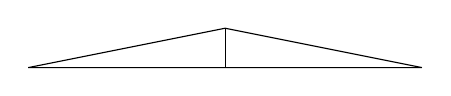
\begin{tikzpicture}[x=1mm, y=1mm]
  \draw (0,0) -- (25,5) -- (50,0) -- cycle;
  \draw (25,0) -- (25,5);
\end{tikzpicture}
\end{koodilohkosis}

\begin{tulossis}
  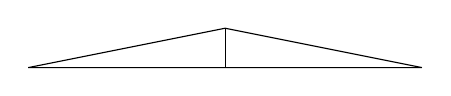
\begin{tikzpicture}[x=1mm, y=1mm]
    \draw (0,0) -- (25,5) -- (50,0) -- cycle;
    \draw (25,0) -- (25,5);
  \end{tikzpicture}
\end{tulossis}

\noindent
Edellisessä esimerkissä ympäristön alussa määritellään hakasulkeissa
perusasetuksia. Tässä asetetaan x- ja y\=/ akselien suuntaiset
yksikkömitat 1\,mm:n pituiseksi. Piirtokomentojen koordinaatit käyttävät
sen jälkeen näitä yksiköitä. Jos yksiköitä ei määritellä, käytetään
oletusyksikköä, joka on 10\,mm. On myös mahdollista antaa
piirtokomentojen koordinaateissa suoraan Latexin mittayksiköt,
esimerkiksi \koodi{(25mm,5mm)} tai \koodi{(10bp,20bp)}, jolloin
koordinaatit tulevat juuri näiden mittojen mukaiseksi. Piirustusalustan
origo eli koordinaatti (0,~0) sijaitsee vasemmassa alanurkassa, ja
koordinaatisto kasvaa ylös ja oikealle.

Edellä olevassa esimerkissä piirretään komennolla \komento{draw}
viivakuvio, jonka välipisteiden koordinaatit ilmaistaan sulkeissa.
Lopussa oleva \koodi{cycle} piirtää viivan takaisin saman
\komento{draw}\-/ komennon alkupisteeseen. Tätä kokonaisuutta kutsutaan
poluksi, ja sen lopussa täytyy olla puolipiste
(\koodi{;}).\footnote{Polkujen luomisen peruskomento on \komento{path},
  joka ei piirrä mitään, ellei sille anna valinnaista argumenttia
  \koodi{draw}. Komento \komento{draw} on itse asiassa sama kuin
  \komento{path}\komentoargv{draw}.} Esimerkissä on toinenkin polku eli
toinen \komento{draw}\-/ komento, joka piirtää pystyviivan suuren
kolmion keskelle ja jakaa sen kahdeksi pienemmäksi kolmioksi.

Koordinaatit voi ilmaista suhteessa polun edelliseen pisteeseen
lisäämällä koordinaattisulkeiden eteen kaksi plusmerkkiä. Seuraavassa
esimerkissä havainnollistetaan sitä. Kuvion (polun) neljä ensimmäistä
pistettä ilmaistaan x- ja y\=/ koordinaateilla mutta viimeinen piste
ilmaistaan kulman (25°) ja pituuden (8) avulla.

\ymparistoi{tikzpicture}
\komentoi{draw}
\begin{koodilohkosis}
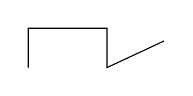
\begin{tikzpicture}[x=1mm, y=1mm]
  \draw (0,0) -- ++(0,5) -- ++(10,0) -- ++(0,-5) -- ++(25:8);
\end{tikzpicture}
\end{koodilohkosis}

\begin{tulossis}
  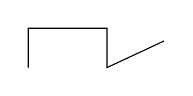
\begin{tikzpicture}[x=1mm, y=1mm]
    \draw (0,0) -- ++(0,5) -- ++(10,0) -- ++(0,-5) -- ++(25:8);
  \end{tikzpicture}
\end{tulossis}

\noindent
Viivojen lisäksi on olemassa komentoja muillekin geometrisille
peruskuvioille. Esimerkissä \ref{esim/tikz-kuvioita} piirretään
suorakulmio, ympyrä, ellipsi, sektorin kaari (0--90°) ja taivutettu
viiva. Viimeksi mainittu (rivi~6) sisältää alkupisteen, kaksi
näkymätöntä ohjauspistettä (\koodi{controls}, \koodi{and}), joiden
suuntaan viivaa taivutetaan, sekä loppupisteen.

\begin{esimerkki*}
  \ymparistoi{tikzpicture}
  \komentoi{draw}

\begin{koodilohko}
\begin{tikzpicture}[x=1mm, y=1mm]
  \draw (0,0) rectangle (10,5);
  \draw (20,2.5) circle [radius=2.5];
  \draw (35,2.5) ellipse [x radius=4, y radius=2, rotate=30];
  \draw (55,0) arc [start angle=0, end angle=90, radius=5];
  \draw (65,0) .. controls (75,7) and (80,7) .. (80,0);
\end{tikzpicture}
\end{koodilohko}

  \begin{tulos}
    \begin{tikzpicture}[x=1mm, y=1mm]
      \draw (0,0) rectangle (10,5);
      \draw (20,2.5) circle [radius=2.5];
      \draw (35,2.5) ellipse [x radius=4, y radius=2, rotate=30];
      \draw (55,0) arc [start angle=0, end angle=90, radius=5];
      \draw (65,0) .. controls (75,7) and (80,7) .. (80,0);
    \end{tikzpicture}
  \end{tulos}

  \caption{Erilaisia geometrisia kuvioita: suorakulmio, ympyrä, ellipsi,
    ympyrän kaari ja taivutettu viiva}
  \label{esim/tikz-kuvioita}
\end{esimerkki*}

Kuten esimerkki \ref{esim/tikz-kuvioita} osoittaa, piirtokomennoille voi
antaa hakasulkeissa lisätietoja. Mahdollisuuksia on valtavan paljon:
esimerkiksi värit, viivojen paksuus, nuolenkärjet ja kulmien pyöristys
ilmaistaan tällaisten lisätietojen avulla. Esimerkki
\ref{esim/tikz-asetuksia} havainnollistaa tavallisimpia valinnaisia
argumentteja. Värivalitsimien \koodi{draw} ja \koodi{fill} arvoksi voi
antaa mitä hyvänsä nimettyjä värejä, joita käsitellään tarkemmin luvussa
\ref{luku/värit}.

\begin{esimerkki*}
  \ymparistoi{tikzpicture}
  \komentoi{draw}

\begin{koodilohko}
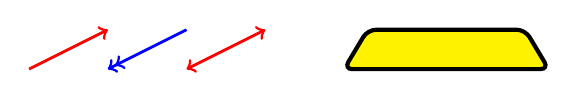
\begin{tikzpicture}[x=1mm, y=1mm,
  nuoli/.style={line width=1bp, draw=red}]

  % Nuolia
  \draw [nuoli, ->] (0,0) -- (10,5);
  \draw [nuoli, <<-, draw=blue] (10,0) -- (20,5);
  \draw [nuoli, <->] (20,0) -- (30,5);

  % Täytetty nelikulmio, viivan paksuus ja kulmien pyöristys
  \draw [draw=black, fill=yellow, line width=1.5bp, rounded
    corners=3bp] (40,0) -- ++(3,5) -- ++(20,0) -- ++(3,-5) -- cycle;
\end{tikzpicture}
\end{koodilohko}

  \begin{tulos}
    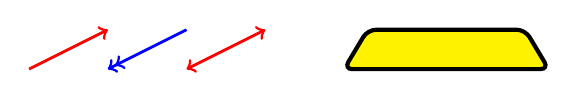
\begin{tikzpicture}[x=1mm, y=1mm,
      nuoli/.style={line width=1bp, draw=red}]

      % Nuolia
      \draw [nuoli, ->] (0,0) -- (10,5);
      \draw [nuoli, <<-, draw=blue] (10,0) -- (20,5);
      \draw [nuoli, <->] (20,0) -- (30,5);

      % Täytetty nelikulmio, viivan paksuus ja kulmien pyöristys
      \draw [draw=black, fill=yellow, line width=1.5bp, rounded
      corners=3bp] (40,0) -- ++(3,5) -- ++(20,0) -- ++(3,-5) -- cycle;
    \end{tikzpicture}
  \end{tulos}

\caption{Erilaisia piirtokomentojen argumentteja: nuolenkärjet, värit,
  viivan paksuus ja kulmien pyöristys}
\label{esim/tikz-asetuksia}
\end{esimerkki*}

Esimerkissä \ref{esim/tikz-asetuksia} olevan \ymparisto{tikzpicture}\-/
ympäristön valinnaisessa argumentissa määritellään rivillä~2 oma
tyyliasetus nimeltä \koodi{nuoli}. Asetukseen kuuluu viivan leveys
(\koodi{line width}) ja väri (\koodi{draw}). Näin määriteltyä
\koodi{nuoli}\-/ tyyliä käytetään rivien 5\==7 \komento{draw}\-/
komennoissa. Tällä tavoin omia tyylejä määrittelemällä säästää
todennäköisesti aikaa ja vaivaa, koska tyyliasetuksia voi sen jälkeen
muuttaa yhdestä paikasta.

Usein tarvittavat \komento{draw}\-/ polut ja komentosarjat kannattanee
piilottaa omien komentojen sisään. Kirjoittaja voi siis tehdä
\komento{newcommand}\-/komennolla (luku \ref{luku/komennot}) ja muilla
vastaavilla omia, mahdollisesti kokeamman tason piirtokomentoja, jotka
piirtävät usein tarvittavia kuvan osia.

\begin{esimerkki*}
  \ymparistoi{tikzpicture}
  \komentoi{node}

\begin{koodilohko}

\begin{tikzpicture}[x=1mm, y=1mm]
  \node at (0,0) [draw=red, rectangle, rounded corners=3bp] {vasen};
  \node [color=blue] at (20,0) {keski};
  \node at (40,0) [draw, circle, inner sep=0bp, fill=yellow] {oikea};
\end{tikzpicture}
\end{koodilohko}

  \begin{tulos}
    
\begin{tikzpicture}[x=1mm, y=1mm]
      \node at (0,0) [draw=red, rectangle, rounded corners=3bp] {vasen};
      \node [color=blue] at (20,0) {keski};
      \node at (40,0) [draw, circle, inner sep=0bp, fill=yellow] {oikea};
    \end{tikzpicture}
  \end{tulos}

  \caption{Solmuja tehdään \komento{node}\-/ komennolla}
  \label{esim/tikz-solmut}
\end{esimerkki*}

Kuvaan voi sisällyttää myös tekstiä tai muuta Latexin sisältöä. Se
tapahtuu helpoimmin komennolla \komento{node}, joka tekee niin sanottuja
solmuja. Komento tarvitsee ainakin solmun sijaintikoordinaatit ja
ladottavan sisällön. Esimerkissä \ref{esim/tikz-solmut} on kolme
erityyppistä solmua.

Kuten esimerkistä näkyy, solmulle voi määrittää kehykset ja niiden
värin, (\koodi{draw}), täyttövärin (\koodi{fill}), sisällön värin
(\koodi{color}), kehyksen kulmien pyöristyksen (\koodi{\englanti{rounded
    corners}}) ja sisäisen tyhjän tilan suuruuden (\koodi{inner sep}).
Kaikenlaista muutakin voi tehdä valinnaiseen argumenttiin
sisällytettävien valitsimien avulla, mutta niistä täytyy lukea lisää
paketin omasta ohjekirjasta.

\begin{esimerkki*}
  \ymparistoi{tikzpicture}
  \komentoi{node}
  \komentoi{draw}

\begin{koodilohko}
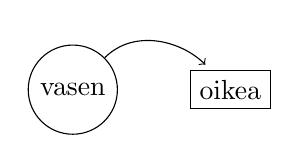
\begin{tikzpicture}[x=1mm, y=1mm]
  \node (ympyrä)      at  (0,0) [draw, circle]    {vasen};
  \node (suorakulmio) at (20,0) [draw, rectangle] {oikea};
  \draw [->, shorten >=1mm] (ympyrä) to [out=45, in=135] (suorakulmio);
\end{tikzpicture}
\end{koodilohko}

  \begin{tulos}
    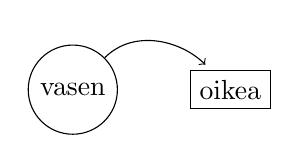
\begin{tikzpicture}[x=1mm, y=1mm]
      \node (ympyrä) at (0,0) [draw, circle] {vasen};
      \node (suorakulmio) at (20,0) [draw, rectangle] {oikea};
      \draw [->, shorten >=1mm] (ympyrä) to [out=45, in=135] (suorakulmio);
    \end{tikzpicture}
  \end{tulos}

  \caption{Solmujen nimeäminen ja kytkeminen viivan avulla}
  \label{esim/tikz-solmujen-yhdistäminen}
\end{esimerkki*}

Solmulle voi määrittää yksilöllisen nimen, jota voi sitten käyttää
esimerkiksi viivojen piirtämiseen solmujen välille. Ei siis tarvitse
käyttää tavallisia \komento{draw}\-/ komennon koordinaatteja vaan voi
käyttää solmulle annettua nimeä. Tätä havainnollistetaan esimerkissä
\ref{esim/tikz-solmujen-yhdistäminen}, jossa esitellään myös
\komento{draw}\-/ komennon \koodi{to}\-/ operaatio. Se mahdollistaa
solmujen välisen viivan lähtö- ja tulokulman valinnan valitsimilla
\koodi{out} ja \koodi{in}. Esimerkissä myös lyhennetään nuolta
loppupäästä käyttämällä valitsinta \koodil{shorten~>}.

Tämän alaluvun ohjeiden avulla pääsee aika mukavasti alkuun
\paketti{tikz}\-/ paketin käytössä ja saa toteutettua tavallisimmat
vektorigrafiikkakuviot. Paketin omaan ohjekirjaan kannattaa silti
tutustua, sillä \ymparisto{tikzpicture}\-/ ympäristön mahdollisuudet
ovat valtavat.

\section{Matematiikka}
\label{luku/matematiikka}

Latexin matematiikkatila on suunniteltu matemaattisten kaavojen
latomiseen eli matematiikan syntaksia varten. Se on aivan oma
todellisuutensa, joka ei tunnu noudattavan samoja sääntöjä kuin
tekstitila. Matematiikkatilassa ovat voimassa eri komennot, eri fontit,
erilainen merkkien käyttäytyminen ja erilaiset välistykset. Tässä
luvussa käsitellään tilan käyttöä ja matemaattisen syntaksin
kirjoittamista. Fonttiasetuksia käsitellään luvussa
\ref{luku/matematiikka-fontit}.

\subsection{Matematiikkatilan käyttö}
\label{luku/matematiikka-käyttö}

Matematiikkatila voidaan kytkeä päälle joko tavallisen, tekstitilassa
toimivan rivin sisällä tai omassa tekstikappaleessaan. Tekstirivillä
matemaattiset kaavat lisätään komentojen \komento{(} ja \komento{)}
väliin, kahden \koodi{\$}\-/ merkin väliin tai ympäristön
\ymparisto{math} sisälle. Seuraavassa on esimerkki kaikista kolmesta:

\begin{koodilohkosis}
Kaava \( y = 2x + 3 \) on suoran yhtälö.
Kaava $y = 2x + 3$ on suoran yhtälö.
Kaava \begin{math} y = 2x + 3 \end{math} on suoran yhtälö.
\end{koodilohkosis}

\begin{tulossis}
Kaava \( y = 2x + 3 \) on suoran yhtälö.
Kaava $y = 2x + 3$ on suoran yhtälö.
Kaava \begin{math} y = 2x + 3 \end{math} on suoran yhtälö.
\end{tulossis}

\noindent
Kuten edellä olevasta esimerkistä näkyy, matematiikkatilassa kirjaimet
ladotaan kursiivilla. Tavalliset lähdetiedostoon kirjoitetut kirjaimet
on tarkoitettu muuttujien nimiksi, kuten tässä esimerkissä $x$ ja~$y$.

Jos matemaattiset kaavat ovat pitkiä tai vievät pystysuuntaista tilaa
enemmän kuin tavallisen rivikorkeuden verran, on parasta latoa ne omaksi
kappaleekseen. Se toteutetaan esimerkiksi kirjoittamalla kaavat
ympäristön \ymparisto{displaymath} sisään tai komentojen \komento{[} ja
\komento{]} väliin. Molemmat toimivat samalla tavalla.

\komentoi{[}
\komentoi{]}
\mkomentoi{left}
\mkomentoi{right}
\mkomentoi{frac}
\begin{koodilohkosis}
\[ \left(\frac{1}{x}\right)^2 = \frac{1}{x^2} \]
\end{koodilohkosis}
\[ \left(\frac{1}{x}\right)^2 = \frac{1}{x^2} \]

\noindent
Ympäristö \ymparisto{equation} toimii muuten samalla tavalla, mutta se
latoo kaavan viereen myös järjestysnumeron ristiviittauksia varten.
Ympäristön sisälle voi kirjoittaa \komento{label}\-/ komennon, jonka
argumentissa annetaan kaavalle yksilöllinen tunniste. Tekstistä voi
viitata kaavaan \komento{ref}\-/ komennolla, jonka argumenttina on
kaavan tunniste. Ristiviittauksia käsitellään tarkemmin luvussa
\ref{luku/ristiviitteet}.

Kaavojen numerot tulevat laskurista \laskuri{equation}, ja numeron
latomiseen voi vaikuttaa määrittelemällä uudelleen komennon
\komento{theequation}. Seuraavassa esimerkissä kaavan numeroon asetetaan
ensiksi \komento{section}\-/ tasoisen otsikon numero, piste erottimeksi
ja lopuksi kyseisen kaavan numero.

\komentoi{renewcommand}
\komentoi{theequation}
\komentoi{thesection}
\komentoi{arabic}
\laskurii{equation}
\begin{koodilohkosis}
\renewcommand{\theequation}{\thesection.\arabic{equation}}
\end{koodilohkosis}

\noindent
Latexin lähdedokumentissa matematiikkatilassa kaavojen täytyy sisältyä
yhteen kappaleeseen eli tyhjiä rivejä ei sallita. Matemaattiset kaavat
ladotaan oletuksena sivun keskelle vaakasuunnassa, mutta jos asettaa
Latexin dokumenttiluokalle (luku
\ref{luku/perusdokumenttiluokat-asetukset}) valitsimen \koodi{fleqn}, ne
ladotaan sivun vasempaan reunaan. Kaavojen numerot ladotaan oletuksena
sivun oikeaan reunaan, mutta vasemmalle ne saa käyttämällä
dokumenttiluokan valitsinta \koodi{leqno}.

Matematiikkaympäristössä on käytettävissä taulukkoympäristö
\mymparisto{array}, joka toimii pitkälti samalla tavalla kuin
tekstitilan taulukotkin (luku \ref{luku/taulukot}). Pelkästään
matematiikkatilassa toimiva \mymparisto{array}\-/ ympäristö mahdollistaa
useiden kaavarivien latomisen ja kohdistamisen vaakasuunnassa tietylle
kohdalle. Esimerkiksi yhtälöt on mielekästä sijoittaa samalle tasalle
yhtäsuuruusmerkin kohdalta.

\mymparistoi{array}
\begin{koodilohkosis}
\[ \begin{array}{r@{~}l}
     4x - 2 &= 6 \\
     x      &= 2 \\
   \end{array} \]
\end{koodilohkosis}
\[ \begin{array}{r@{~}l}
     4x - 2 &= 6 \\
     x      &= 2 \\
   \end{array} \]

\noindent
Pidemmälle kehitettyjä matematiikkaympäristöjä on paketissa
\pakettictan{amsmath}. Esimerkiksi \ymparisto{align}\-/\ ja
\ymparisto{align*}\-/ ympäristöt pystyvät tasaamaan allekkaiset kaavat
tietystä kohdasta, eikä taulukon sarakkeita tarvitse erikseen
määritellä. Tasauskohta ilmaistaan lähdedokumentissa \koodi{\&}\=/
merkillä normaalien taulukoiden tavoin. Ympäristön tähtiversio
\ymparisto{align*} ei lado kaavan numeroa mukaan. Edellä olleen
yhtälöesimerkin voi toteuttaa yksinkertaisemmin seuraavasti:

\ymparistoi{align*}
\begin{koodilohkosis}
\begin{align*}
  4x - 2 &= 6 \\
  x      &= 2
\end{align*}
\end{koodilohkosis}

\noindent
Edellä mainittuja \ymparisto{align}\-/\ ja \ymparisto{align*}\-/
ympäristöjä ei kirjoiteta komentojen \komento{[} ja \komento{]} sisään,
eli nämä ympäristöt on tarkoitettu tekstitilassa käytettäväksi.
Ympäristön sisältö on matematiikkatilassa.

Paketti \paketti{amsmath} sisältää paljon muitakin hyödyllisiä
ympäristöjä ja komentoja matematiikan latomiseen. Paketin ohjekirjaan on
erittäin suositeltavaa tutustua.

\subsection{Matematiikkatilan kielioppia}

Matematiikan kirjoittaminen Latexissa on tehty varsin luonnolliseksi.
Esimerkiksi tavalliset operaattorit ja kokonaisluvut kirjoitetaan
näppäimistöltä sellaisenaan, ja jos desimaalierottimena on piste, sekin
syötetään näppäimistöltä suoraan. Suomessa käytetään desimaalierottimena
kuitenkin pilkkua, joka toimii Latexin matematiikkatilassa välimerkkinä:
sen jälkeen ladotaan pieni väli. Suomalaisen desimaalierottimen saa
kirjoittamalla pilkun ympärille aaltosulkeet.

\mkomentoi{pi}
\mkomentoi{approx}
\begin{koodilohkosis}
\[ \pi \approx 3{,}142 \]
\end{koodilohkosis}
\[ \pi \approx 3{,}142 \]

\noindent
Toinen vaihtoehto pilkun käyttämiseen desimaalierottimana on ladata
paketti \pakettictan{icomma}. Paketti määrittelee matematiikkatilan
pilkun toimimaan jokseenkin älykkäästi: jos lähdetiedostossa on pilkun
jälkeen väli, pilkku ladotaan välimerkkinä; jos väliä ei ole, pilkku
katsotaan desimaalierottimeksi.

Plus-, jako- ja yhtäsuuruusmerkki sekä pienempi kuin ja suurempi kuin
\=/merkit ($+ : / = \; < \; >$) kirjoitetaan näppäimistöltä
sellaisenaan. Miinusmerkki ($-$) kirjoitetaan yhdysmerkin (\koodi{-})
avulla, eli yhdysmerkki ladotaan dokumenttiin Unicode\-/ merkistön
miinusmerkkinä \uctunnus{u+2212 minus sign}. Kertomerkit voi kirjoittaa
lähdedokumenttiin sellaisenaan mutta myös komennoilla \mkomento{cdot}
($\cdot$) ja \mkomento{times} ($\times$).

Pienet sulkeetkin voi kirjoittaa näppäimistöltä suoraan, mutta
matematiikassa tarvitaan usein erikokoisia, tilanteeseen mukautuvia
sulkeita. Ne tehdään komentojen \mkomento{left} (vasen) ja
\mkomento{right} (oikea) avulla. Komentojen jälkeen kirjoitetaan haluttu
suljemerkki, esimerkiksi \mkomento{left}\mkomentojatko{(} ja
\mkomento{right}\mkomentojatko{)}. Itseisarvoa merkitsevät pystyviivat
tehdään samoilla komennoilla, mutta suljemerkkien tilalle kirjoitetaan
pystyviiva~(\koodi{|}).

\mkomentoi{left}
\mkomentoi{right}
\mkomentoi{frac}
\begin{koodilohkosis}
\[ \left| a + \left( \frac{b}{c \left( d-1 \right)} \right) \right| \]
\end{koodilohkosis}
\[ \left| a + \left( \frac{b}{c \left( d-1 \right)} \right) \right| \]

\noindent
Komentoja \mkomento{left} ja \mkomento{right} täytyy käyttää pareittain,
jotta Latex osaa latoa oikeankokoiset sulkeet. Jos ei halua
suljemerkille paria, kirjoitetaan toisen suljekomennon ''sulkeeksi''
piste. Seuraavassa esimerkissä ladotaan vasemmalle aaltosulje
(\mkomento{left}\mkomentojatko{\keno\{}) mutta oikealle ei mitään
(\mkomento{right}\mkomentojatko{.}).

\mkomentoi{left}
\mkomentoi{right}
\mymparistoi{array}
\begin{koodilohkosis}
\[ \left\{ \begin{array}{r@{~}l}
             x &= 4 \\
             y &= -2 \\
           \end{array} \right. \]
\end{koodilohkosis}
\[ \left\{ \begin{array}{l@{~}l}
             x &= 4 \\
             y &= -2 \\
           \end{array} \right. \]

\noindent
Matematiikkatilan ylä- ja alaindeksit toteutetaan sirkumfleksin
(\koodi{\^{}}) ja alaviivan (\koodi{\_}) avulla. Välittömästä merkin
jälkeen oleva merkki ladotaan ylä- tai alaindeksiksi, ja jos indeksi
sisältää enemmän kuin yhden merkin, kirjoitetaan kokonaisuus
aaltosulkeisiin. Joidenkin matemaattisten operaattorikomentojen
yhteydessä indeksit ladotaan poikkeuksellisella tavalla, esimerkiksi
kokonaan operaattorin ylä- tai alapuolelle.

\mkomentoi{sum}
\mkomentoi{int}
\mkomentoi{lim}
\mkomentoi{to}
\mkomentoi{infty}
\mkomentoi{qquad}
\begin{koodilohkosis}
\[ x^{n-1} \qquad x_i \qquad \sum_{i=1}^n \qquad
  \int_0^\infty \qquad \lim_{n \to \infty} \]
\end{koodilohkosis}
\[ x^{n-1} \qquad x_i \qquad \sum_{i=1}^n \qquad
  \int_0^\infty \qquad \lim_{n \to \infty} \]

\noindent
Lausekkeen osia voi ryhmitellä ylä- tai alapuolisella aaltosulkeella,
jotka tehdään komennoilla \mkomento{overbrace} ja \mkomento{underbrace}.
Jos näiden komentojen jälkeen käyttää ylä- tai alaindeksiä, se ladotaan
sulkeen keskelle. Seuraavassa on esimerkki:

\mkomentoi{overbrace}
\mkomentoi{underbrace}
\begin{koodilohkosis}
\[ \overbrace{3x + x}^{4x} - \underbrace{5y - 2y}_{3y} = 4x - 3y \]
\end{koodilohkosis}
\[ \overbrace{3x + x}^{4x} - \underbrace{5y - 2y}_{3y} = 4x - 3y \]

\noindent
Muuttujien, funktion nimien tai muiden symbolien jäljessä oleva
$'$\=/merkki tehdään yleisheittomerkin (\koodi{'}) avulla.
Matematiikassa se voi tarkoittaa esimerkiksi funktion
derivaattafunktiota, ja Unicode\-/ merkistössä merkin tunnus
\uctunnus{u+2032 prime}.

\mkomentoi{quad}
\begin{koodilohkosis}
\[ f(x) = 3x^2 - 2x \quad f'(x) = 6x - 2 \]
\end{koodilohkosis}
\[ f(x) = 3x^2 - 2x \quad f'(x) = 6x - 2 \]

\noindent
Murtoluvuille ja jakoviivan latomiseen on komento \mkomento{frac}, jolle
annetaan kaksi argumenttia: osoittaja ja nimittäjä. Neliö- ja muut
juuret tehdään \mkomento{sqrt}\-/ komennolla, jolle annetaan ainakin
yksi argumentti. Komennolle voi antaa hakasulkeissa toisenkin
argumentin, joka ilmaisee juuriluvun. Seuraavassa on esimerkki
murtoluvun, neliöjuuren ja kuutiojuuren toteuttamisesta:

\mkomentoi{frac}
\mkomentoi{sqrt}
\mkomentoi{quad}
\begin{koodilohkosis}
\[ \frac{1}{3x + 1} \quad \sqrt{9} = \sqrt[3]{27} \]
\end{koodilohkosis}
\[ \frac{1}{3x + 1} \quad \sqrt{9} = \sqrt[3]{27} \]

\noindent
Vektorien nimien latomiseen eli merkkien yläpuoliselle nuolelle on oma
komento \mkomento{vec}, joka toimii yhden kirjaimen kanssa. Kahden
merkin mittaiseen nuoleen tarvitaan komentoa \mkomento{overrightarrow}
(tai \mkomento{overleftarrow}).

\mkomentoi{vec}
\mkomentoi{overrightarrow}
\mkomentoi{quad}
\begin{koodilohkosis}
\[ \vec{a} \quad \overrightarrow{AB} \]
\end{koodilohkosis}
\[ \vec{a} \quad \overrightarrow{AB} \]

\noindent
Matriisit voi toteuttaa luvussa \ref{luku/matematiikka-käyttö} esitellyn
\mymparisto{array}\-/ ympäristön avulla, mutta kätevämpää on käyttää
\paketti{amsmath}\-/ paketin ympäristöjä. Kullekin erilaiselle
suljetyypille on oma ympäristönsä: \mymparisto{matrix},
\mymparisto{pmatrix}~$(\,)$, \mymparisto{bmatrix}~$[\,]$,
\mymparisto{Bmatrix}~$\{\,\}$, \mymparisto{vmatrix}~$|$ ja
\mymparisto{Vmatrix}~$\|$. Ympäristön sisällä matriisin rivin solut
erotetaan toisistaan samoin kuin taulukoissakin eli \koodi{\&}\=/
merkillä ja rivinvaihto tehdään \mkomento{\keno}\=/ komennolla.
Seuraavassa on esimerkki kahdesta eri ympäristöstä:

\mymparistoi{matrix}
\mymparistoi{bmatrix}
\mkomentoi{qquad}
\begin{koodilohkosis}
\[ \begin{matrix} 1 & 2 \\ 3 & 4 \\ \end{matrix} \qquad
   \begin{bmatrix}
     1 & 2 & 3 \\ 4 & 5 & 6 \\ 7 & 8 & 9 \\
   \end{bmatrix} \]
\end{koodilohkosis}
\[ \begin{matrix} 1 & 2 \\ 3 & 4 \\ \end{matrix} \qquad
  \begin{bmatrix}
    1 & 2 & 3 \\ 4 & 5 & 6 \\ 7 & 8 & 9 \\
  \end{bmatrix} \]

\leijutlk{
  \providecommand{\rivi}{}
  \renewcommand{\rivi}[3]{\mkomento{#1} & $#2$ & #3 \\}

  \begin{tabular}{lll}
    \toprule
    \ots{Komento}
    & \ots{Esimerkki}
    & \ots{Merkitys} \\
    \midrule
    \rivi{mathrm}{\mathrm{ABC~abc}}{antiikva, serif, roman}
    \rivi{mathsf}{\mathsf{ABC~abc}}{groteski, sans serif, gothic}
    \rivi{mathtt}{\mathtt{ABC~abc}}{tasalevyinen, typewriter}
    \rivi{mathcal}{\mathcal{ABC}}{kalligrafinen}
    \midrule
    \rivi{mathbf}{\mathbf{ABC~abc}}{lihavoitu, bold}
    \rivi{mathit}{\mathit{ABC~abc}}{kursiivi, italic}
    \bottomrule
  \end{tabular}
}{
  \caption{Tekstin latominen matematiikkatilassa vaatii erityisen
    komennon}
  \label{tlk/matem-teksti}
}

\noindent
Kuten on jo todettu, tavalliset kirjaimet on matematiikkatilassa
tarkoitettu muuttujien nimiksi. Kun täytyy latoa varsinaista tekstiä --
tekstitilan tavoin -- täytyy käyttää erityisiä komentoja. Taulukkoon
\ref{tlk/matem-teksti} on koottu matematiikkatilan
tekstinlatomiskomentoja. Komentojen argumenttina oleva teksti ladotaan
kuin tekstitilassa.

Vaakasuuntaisten välien tekemiseen on matematiikkatilassa muutama
komento. Komento \mkomento{quad} latoo typografisen neliön (1\,em)
levyisen välin. Se on sama kuin nykyisen fontin koko. Komento
\mkomento{qquad} latoo 2\,em:n levyisen välin. Pienempiä välejä saa
komennoilla \mkomento{,} (\murtoluku{3}{18}\,em), \mkomento{:}
(\murtoluku{4}{18}\,em) ja \mkomento{;} (\murtoluku{5}{18}\,em). Komento
\mkomento{!} puolestaan tuottaa negatiivisen välin, jonka mitta on
−\murtoluku{3}{18}\,em. Negatiivista väliä voi käyttää liian suuren
välin pienentämiseen.

\subsection{Erikoismerkkejä}

Matematiikkatilassa voi käyttää Unicode\-/ merkistöä, eli monet
matemaattiset symbolit voi kirjoittaa lähdedokumenttiin sellaisenaan.
Voi silti olla helpompaa käyttää erityisiä komentoja sellaisten
kirjainten ja symbolien kirjoittamiseen, joita ei ihan helposti pysty
tuottamaan näppäimistöltä tai tekstieditorin toimintojen avulla.
Matematiikkatilan erikoismerkkejä on koottu oheisiin taulukoihin
(\ref{tlk/matem-kreikk}--). Lisää symboleja on paketeissa
\pakettictan{latexsym} ja \pakettictan{amsmath}.

\leijutlk{
  \providecommand{\rivi}{}
  \renewcommand{\rivi}[2]{$#1$ & \mkomento{#2}}

  \begin{tabular}{*{4}{cl}}
    \toprule

    \rivi{\alpha}{alpha}
    & \rivi{\Alpha}{Alpha}
    & \rivi{\beta}{beta}
    & \rivi{\Beta}{Beta} \\

    \rivi{\gamma}{gamma}
    & \rivi{\Gamma}{Gamma}
    & \rivi{\delta}{delta}
    & \rivi{\Delta}{Delta} \\

    \rivi{\epsilon}{epsilon}
    & \rivi{\varepsilon}{varepsilon}
    & \rivi{\Epsilon}{Epsilon}
    & \rivi{\zeta}{zeta} \\

    \rivi{\Zeta}{Zeta}
    & \rivi{\eta}{eta}
    & \rivi{\Eta}{Eta}
    & \rivi{\theta}{theta} \\

    \rivi{\vartheta}{vartheta}
    & \rivi{\Theta}{Theta}
    & \rivi{\iota}{iota}
    & \rivi{\Iota}{Iota} \\

    \rivi{\kappa}{kappa}
    & \rivi{\Kappa}{Kappa}
    & \rivi{\lambda}{lambda}
    & \rivi{\Lambda}{Lambda} \\

    \rivi{\mu}{mu}
    & \rivi{\Mu}{Mu}
    & \rivi{\nu}{nu}
    & \rivi{\Nu}{Nu} \\

    \rivi{\xi}{xi}
    & \rivi{\Xi}{Xi}
    & \rivi{\pi}{pi}
    & \rivi{\varpi}{varpi} \\

    \rivi{\Pi}{Pi}
    & \rivi{\rho}{rho}
    & \rivi{\varrho}{varrho}
    & \rivi{\Rho}{Rho} \\

    \rivi{\sigma}{sigma}
    & \rivi{\varsigma}{varsigma}
    & \rivi{\Sigma}{Sigma}
    & \rivi{\tau}{tau} \\

    \rivi{\Tau}{Tau}
    & \rivi{\upsilon}{upsilon}
    & \rivi{\Upsilon}{Upsilon}
    & \rivi{\phi}{phi} \\

    \rivi{\varphi}{varphi}
    & \rivi{\Phi}{Phi}
    & \rivi{\chi}{chi}
    & \rivi{\Chi}{Chi} \\

    \rivi{\psi}{psi}
    & \rivi{\Psi}{Psi}
    & \rivi{\omega}{omega}
    & \rivi{\Omega}{Omega} \\

    \bottomrule
  \end{tabular}
}{
  \caption{Kreikkalaisten kirjainten latominen matematiikkatilassa}
  \label{tlk/matem-kreikk}
}

\leijutlk{
  \providecommand{\rivi}{}
  \renewcommand{\rivi}[3][a]{$#2{#1}$ & \mkomento{#3}\mkomentoarg{#1}}

  \begin{tabular}{*{3}{cl}}
    \toprule

    \rivi{\grave}{grave}
    & \rivi{\ddot}{ddot}
    & \rivi{\hat}{hat} \\

    \rivi{\acute}{acute}
    & \rivi{\check}{check}
    & \rivi[aaa]{\widehat}{widehat} \\

    \rivi{\breve}{breve}
    & \rivi{\dot}{dot}
    & \rivi{\tilde}{tilde} \\

    \rivi{\bar}{bar}
    & \rivi{\mathring}{mathring}
    & \rivi[aaa]{\widetilde}{widetilde} \\

    \bottomrule
  \end{tabular}
}{
  \caption{Matematiikkatilan tarkekomentoja}
  \label{tlk/matem-tarkkeita}
}

\leijutlk{
  \providecommand{\rivi}{}
  \renewcommand{\rivi}[3][AB]{$#2{#1}$ & \mkomento{#3}\mkomentoarg{#1}}
  \renewcommand{\arraystretch}{1.5}

  \begin{tabular}{*{2}{cl}}
    \toprule

    \rivi{\overrightarrow}{overrightarrow}
    & \rivi{\overleftarrow}{overleftarrow} \\

    \rivi{\underrightarrow}{underrightarrow}
    & \rivi{\underleftarrow}{underleftarrow} \\

    \rivi{\overleftrightarrow}{overleftrightarrow}
    & \rivi{\underleftrightarrow}{underleftrightarrow} \\

    \rivi{\overline}{overline}
    & \rivi{\underline}{underline} \\

    \rivi[abc]{\overbrace}{overbrace}
    & \rivi[abc]{\underbrace}{underbrace} \\

    \bottomrule
  \end{tabular}
}{
  \caption{Ylä- ja alamerkintöjä}
  \label{tlk/matem-yla-ala-merk}
}

\leijutlk{
  \providecommand{\rivi}{}
  \renewcommand{\rivi}[2]{$#1$ & \mkomento{#2}}

  \begin{tabular}{*{4}{cl}}
    \toprule

    $<$
    & \koodi{<}
    & $>$
    & \koodi{>}
    & $=$
    & \koodi{=}
    & $:$
    & \koodi{:} \\

    $\leq$
    & \mkomento{leq}, \mkomento{le}
    & $\geq$
    & \mkomento{geq}, \mkomento{ge}
    & \rivi{\ll}{ll}
    & \rivi{\gg}{gg} \\

    \rivi{\equiv}{equiv}
    & \rivi{\doteq}{doteq}
    & \rivi{\prec}{prec}
    & \rivi{\preceq}{preceq} \\

    \rivi{\succ}{succ}
    & \rivi{\succeq}{succeq}
    & \rivi{\sim}{sim}
    & \rivi{\simeq}{simeq} \\

    \rivi{\subset}{subset}
    & \rivi{\subseteq}{subseteq}
    & \rivi{\supset}{supset}
    & \rivi{\supseteq}{supseteq} \\

    \rivi{\approx}{approx}
    & \rivi{\cong}{cong}
    & \rivi{\sqsubset}{sqsubset}
    & \rivi{\sqsubseteq}{sqsubseteq} \\

    \rivi{\sqsupset}{sqsupset}
    & \rivi{\sqsupseteq}{sqsupseteq}
    & \rivi{\bowtie}{bowtie}
    & \rivi{\in}{in} \\

    \rivi{\ni}{ni}
    & \rivi{\propto}{propto}
    & \rivi{\vdash}{vdash}
    & \rivi{\dashv}{dashv} \\

    \rivi{\models}{models}
    & \rivi{\mid}{mid}
    & \rivi{\parallel}{parallel}
    & \rivi{\perp}{perp} \\

    \rivi{\smile}{smile}
    & \rivi{\frown}{frown}
    & \rivi{\asymp}{asymp}
    & \rivi{\notin}{notin} \\

    $\neq$
    & \mkomento{neq}, \mkomento{ne} \\

    \bottomrule
  \end{tabular}
}{
  \caption{Relaatioita. Negaation saa kirjoittamalla komennon eteen
    \mkomento{not}}
  \label{tlk/matem-relaatioita}
}

\leijutlk{
  \providecommand{\rivi}{}
  \renewcommand{\rivi}[2]{$#1$ & \mkomento{#2}}
  \renewcommand{\arraystretch}{1.1}

  \begin{tabular}{*{4}{cl}}
    \toprule

    $+$
    & \koodi{+}
    & $-$
    & \koodi{-}
    & \rivi{\pm}{pm}
    & \rivi{\mp}{mp} \\

    \rivi{\cdot}{cdot}
    & \rivi{\div}{div}
    & \rivi{\times}{times}
    & \rivi{\setminus}{setminus} \\

    \rivi{\cup}{cup}
    & \rivi{\cap}{cap}
    & \rivi{\sqcup}{sqcup}
    & \rivi{\sqcap}{sqcap} \\

    \rivi{\vee}{vee}
    & \rivi{\wedge}{wedge}
    & \rivi{\oplus}{oplus}
    & \rivi{\ominus}{ominus} \\

    \rivi{\odot}{odot}
    & \rivi{\oslash}{oslash}
    & \rivi{\uplus}{uplus}
    & \rivi{\otimes}{otimes} \\

    \rivi{\sum}{sum}
    & \rivi{\prod}{prod}
    & \rivi{\coprod}{coprod}
    & \rivi{\int}{int} \\

    \rivi{\oint}{oint}
    & \rivi{\lim}{lim}
    & \rivi{\bigoplus}{bigoplus}
    & \rivi{\bigotimes}{bigotimes} \\

    \rivi{\bigodot}{bigodot}
    & \rivi{\bigvee}{bigvee}
    & \rivi{\bigwedge}{bigwedge}
    & \rivi{\bigcup}{bigcup} \\

    \rivi{\bigcap}{bigcap}
    & \rivi{\biguplus}{biguplus}
    & \rivi{\bigsqcup}{bigsqcup} \\

    \bottomrule
  \end{tabular}
}{
  \caption{Operaattoreita}
  \label{tlk/matem-operaattoreita}
}

\leijutlk{
  \providecommand{\rivi}{}
  \renewcommand{\rivi}[2]{$#1$ & \mkomento{#2}}

  \begin{tabular}{*{2}{cl}}
    \toprule

    $\leftarrow$
    & \mkomento{leftarrow}, \mkomento{gets}
    & $\rightarrow$
    & \mkomento{rightarrow}, \mkomento{to} \\

    \rivi{\longleftarrow}{longleftarrow}
    & \rivi{\longrightarrow}{longrightarrow} \\

    \rivi{\leftrightarrow}{leftrightarrow}
    & \rivi{\longleftrightarrow}{longleftrightarrow} \\

    \rivi{\Leftarrow}{Leftarrow}
    & \rivi{\Rightarrow}{Rightarrow} \\

    \rivi{\Longleftarrow}{Longleftarrow}
    & \rivi{\Longrightarrow}{Longrightarrow} \\

    \rivi{\Leftrightarrow}{Leftrightarrow}
    & \rivi{\Longleftrightarrow}{Longleftrightarrow} \\

    \rivi{\mapsto}{mapsto}
    & \rivi{\longmapsto}{longmapsto} \\

    \rivi{\hookleftarrow}{hookleftarrow}
    & \rivi{\hookrightarrow}{hookrightarrow} \\

    \rivi{\leftharpoonup}{leftharpoonup}
    & \rivi{\rightharpoonup}{rightharpoonup} \\

    \rivi{\leftharpoondown}{leftharpoondown}
    & \rivi{\rightharpoondown}{rightharpoondown} \\

    \rivi{\rightleftharpoons}{rightleftharpoons}
    & \rivi{\iff}{iff} \\

    \rivi{\uparrow}{uparrow}
    & \rivi{\downarrow}{downarrow} \\

    \rivi{\updownarrow}{updownarrow}
    & \rivi{\Updownarrow}{Updownarrow} \\

    \rivi{\Uparrow}{Uparrow}
    & \rivi{\Downarrow}{Downarrow} \\

    \rivi{\nearrow}{nearrow}
    & \rivi{\searrow}{searrow} \\

    \rivi{\swarrow}{swarrow}
    & \rivi{\nwarrow}{nwarrow} \\

    \bottomrule
  \end{tabular}
}{
  \caption{Nuolia}
  \label{tlk/matem-nuolia}
}

\leijutlk{
  \providecommand{\rivi}{}
  \renewcommand{\rivi}[2]{$#1$ & \mkomento{#2}}

  \begin{tabular}{*{4}{cl}}
    \toprule

    \rivi{\langle}{langle}
    & \rivi{\rangle}{rangle}
    & \rivi{\lfloor}{lfloor}
    & \rivi{\rfloor}{rfloor} \\

    \rivi{\rceil}{rceil}
    & \rivi{\lceil}{lceil}
    & $|$
    & \koodi{|}, \mkomento{vert}
    & $\|$
    & \mkomentox{|}, \mkomento{Vert} \\

    \rivi{\lgroup}{lgroup}
    & \rivi{\rgroup}{rgroup}
    & \rivi{\lmoustache}{lmoustache}
    & \rivi{\rmoustache}{rmoustache} \\

    $/$
    & \koodi{/}
    & \rivi{\backslash}{backslash} \\

    \bottomrule
  \end{tabular}
}{
  \caption{Sulkeita ja erotinmerkkejä}
  \label{tlk/matem-erottimia}
}

\leijutlk{
  \providecommand{\rivi}{}
  \renewcommand{\rivi}[2]{$#1$ & \mkomento{#2}}

  \begin{tabular}{*{3}{cl}}
    \toprule

    $\neg$
    & \mkomento{neg}, \mkomento{lnot}
    & \rivi{\angle}{angle}
    & \rivi{\emptyset}{emptyset} \\

    \rivi{\infty}{infty}
    & $'$
    & \koodi{'}
    & \rivi{\prime}{prime} \\

    \rivi{\forall}{forall}
    & \rivi{\exists}{exists}
    & \rivi{\wr}{wr} \\

    \rivi{\bot}{bot}
    & \rivi{\top}{top}
    & \rivi{\surd}{surd} \\

    \rivi{\dots}{dots}
    & \rivi{\cdots}{cdots}
    & \rivi{\vdots}{vdots} \\

    \rivi{\ddots}{ddots}
    & \rivi{\triangle}{triangle}
    & \rivi{\triangleleft}{triangleleft} \\

    \rivi{\triangleright}{triangleright}
    & \rivi{\nabla}{nabla}
    & \rivi{\star}{star} \\

    \rivi{\ast}{ast}
    & \rivi{\circ}{circ}
    & \rivi{\bigcirc}{bigcirc} \\

    \rivi{\bullet}{bullet}
    & \begin{tikzpicture} % \diamond puuttuu fontista
      \draw [rotate=45] (0,0) rectangle (.5ex,.5ex);
    \end{tikzpicture}
    & \mkomento{diamond}
    & \rivi{\amalg}{amalg} \\

    \rivi{\bigtriangleup}{bigtriangleup}
    & \rivi{\bigtriangledown}{bigtriangledown}
    & \rivi{\dagger}{dagger} \\

    \rivi{\ddagger}{ddagger}
    & \rivi{\diamondsuit}{diamondsuit}
    & \rivi{\heartsuit}{heartsuit} \\

    \rivi{\clubsuit}{clubsuit}
    & \rivi{\spadesuit}{spadesuit}
    & \rivi{\flat}{flat} \\

    \rivi{\natural}{natural}
    & \rivi{\sharp}{sharp}
    & \rivi{\hbar}{hbar} \\

    \rivi{\imath}{imath}
    & \rivi{\jmath}{jmath}
    & \rivi{\ell}{ell} \\

    \rivi{\Re}{Re}
    & \rivi{\Im}{Im}
    & \rivi{\aleph}{aleph} \\

    \rivi{\wp}{wp} \\

    \bottomrule
  \end{tabular}
}{
  \caption{Sekalaisia symboleja}
  \label{tlk/matem-sekalaisia}
}
